\documentclass[twoside]{article}
\usepackage{amsfonts,amssymb,amsbsy,textcomp,
  marvosym,picins,amsmath,caption,
  threeparttable,amsthm,subfigure}
\usepackage{eurosym,mathrsfs,fancyhdr,CJK,
  multicol,graphics,indentfirst,color,bm,
  upgreek,booktabs,graphicx}

% users add 
\usepackage{url}
\usepackage[all]{xy}
\usepackage{extarrows}
\usepackage{proof}
\usepackage{hyperref}
\usepackage{wrapfig}
\usepackage{multirow}
\usepackage{epstopdf}
\usepackage{bbm}
\usepackage{tikz}
\usepackage{rotating}
\usepackage{stmaryrd}
\usepackage{enumerate}
\usepackage{stfloats}
\usepackage[section]{placeins}

% new defined Macro
\newcommand{\etal}[1]{{#1} \textit{et al}.}
\newcommand\eg[0]{\textit{e.g.}}
\newcommand\ie[0]{\textit{i.e.}}
\newcommand{\Def}[1]{\text{Def}. {#1}}
\newcommand{\TYPE}[1]{\text{#1}}
\newcommand{\evtabort}{\textbf{abort}}

\newcommand{\circrightarrow}[1]{\ \circ\mkern-7mu\xrightarrow{#1}}
\newcommand{\ptrightarrow}[1]{\ \bullet\mkern-7mu\xrightarrow{#1}}
\newcommand{\maprightarrow}[1]{|\mkern-8mu\longrightarrow^{#1}}
\newcommand{\sepconj}{\wedge \mkern-13mu \wedge}
\newcommand{\sepdisj}{\vee \mkern-13mu \vee}

\newcommand{\dlylsexcarrow}{\rightarrow \mkern-13mu \rightarrow}

\newcommand{\nil}{\text{nil}}

\newcommand\xorOP[0]{\oplus}

\newcommand{\pc}{\texttt{pc}}
\newcommand{\npc}{\texttt{npc}}
\newcommand{\sparc}{\text{SPARCv8}}
\newcommand{\dom}{\text{dom}}

%\newcommand{\state}{S}
\newcommand{\prog}[0]{\text{P}}
\newcommand{\rst}{Q}
\newcommand{\rf}{R}
\newcommand{\fmls}{F}
\newcommand{\code}{C}

\newcommand\Cspec[0]{\Psi}
\newcommand\Bspec[0]{\theta}

% register Macro
\newcommand\RAreg[0]{\reg{15}} % register for return address
\newcommand{\regN}[0]{\texttt{rn}}
\newcommand{\psr}[0]{\texttt{psr}}
\newcommand\regr[0]{\texttt{r}}
\newcommand{\reg}[1]{\texttt{r}_{#1}}
\newcommand{\asr}{\texttt{asr}}
\newcommand{\regn}{\texttt{n}}
\newcommand{\regz}{\texttt{z}}
\newcommand{\regv}{\texttt{v}}
\newcommand{\regc}{\texttt{c}}
\newcommand{\regY}{\texttt{Y}}
\newcommand{\sr}{\texttt{sr}}
\newcommand{\RFile}[0]{R}
\newcommand{\DBuf}[0]{D}
\newcommand\mem[0]{M}
\newcommand{\Wstack}[0]{F}


\newcommand{\word}[0]{w}
\newcommand{\val}[0]{v}
\newcommand\tick[0]{t}
\newcommand{\loc}[0]{l}
\newcommand{\state}[0]{S}
\newcommand{\Rstate}[0]{Q}

\newcommand{\cwp}{w_{\textit{id}}}

\newcommand{\ireg}[1]{\%\texttt{i}_{#1}}
\newcommand{\lreg}[1]{\%\texttt{l}_{#1}}
\newcommand{\oreg}[1]{\%\texttt{o}_{#1}}
\newcommand{\greg}[1]{\%\texttt{g}_{#1}}
\newcommand{\spreg}{\%\texttt{sp}}

\newcommand{\fm}{\text{fm}}

\newcommand{\regwim}{\texttt{wim}}
\newcommand{\regcwp}{\texttt{cwp}}

\newcommand\nextcwp[0]{\textbf{next\_cwp}}
\newcommand\prevcwp[0]{\textbf{prev\_cwp}}
\newcommand{\precwp}{\nextcwp}
\newcommand{\postcwp}{\prevcwp}
%\newcommand{\precwp}{\textbf{pre\_cwp}}
%\newcommand{\postcwp}{\textbf{post\_cwp}}

\newcommand{\winmask}{\textbf{win\_mask}}
\newcommand{\setwin}{\textbf{set\_win}}

\newcommand{\setdelay}{\textbf{set\_delay}}
\newcommand{\exedelay}{\textbf{exe\_delay}}
\newcommand\Dstep[2]{{#1}\rightrightarrows{#2}}
\newcommand\DstepN[3]{{#2}\rightrightarrows^{#1}{#3}}

\newcommand{\letin}[2]{\textbf{let} \; {#1} \; \textbf{in} \; {#2}}

\newcommand{\wfcblk}[4]{\Psi \vdash \{({#1}, {#2})\} \; {#3} : \, {#4}}
\newcommand{\wfins}[3]{\vdash \{{#1}\} \, {#2} \, \{{#3}\}}

\newcommand{\lgvl}{\iota}
\newcommand{\aexp}{\texttt{a}}
\newcommand{\oexp}{\texttt{o}}

\newcommand{\cblk}{\mathbb{I}}
\newcommand{\lab}[1]{\texttt{f}_{#1}}

% model
\newcommand{\asrtmodel}[2]{{#1}\!\models\!{#2}}

% operation macro
\newcommand{\xor}{\textbf{xor}}

% command macro
\newcommand\simplins{\texttt{i}}
\newcommand\jmpl{\texttt{jmpl}}
\newcommand\be{\texttt{be}}
\newcommand\call{\texttt{call}}
\newcommand\retl{\texttt{retl}}
\newcommand\nop{\texttt{nop}}
\newcommand\ld{\texttt{ld}}
\newcommand\st{\texttt{st}}
\newcommand\csave{\texttt{save}}
\newcommand\crestore{\texttt{restore}}
\newcommand\rd{\texttt{rd}}
\newcommand\cwr{\texttt{wr}}
\newcommand\mov{\texttt{mov}}
\newcommand\cadd{\texttt{add}}
\newcommand\csll{\texttt{sll}}
\newcommand\csrl{\texttt{srl}}
\newcommand\cor{\texttt{or}}
\newcommand\andcc{\texttt{andcc}}
\newcommand\bnz{\texttt{bnz}}
\newcommand\rett{\texttt{rett}}
\newcommand\ret{\texttt{ret}}
\newcommand\jmp{\texttt{jmp}}

% operational semantics
\newcommand{\ptrans}[2]{C \vdash {#1} \longmapsto {#2}}
\newcommand{\lptrans}[3]{{#1} \vdash {#2} \longmapsto {#3}}
\newcommand{\cttrans}[2]{C \vdash {#1}  \circrightarrow{\quad} {#2}}
\newcommand\ccttrans[3]{{#1} \vdash {#2} \circrightarrow{\quad} {#3}}
\newcommand{\swtrans}[3]{{#1} \ptrightarrow{{#2}} {#3}}
\newcommand{\itrans}[3]{{#1} \xrightarrow{{#2}} {#3}}

% operations for save and restore
%\newcommand{\decwin}[1]{\textbf{dec\_win}{#1}}
%\newcommand{\incwin}[1]{\textbf{inc\_win}{#1}}
\newcommand{\decwin}[1]{\textbf{save}{#1}}
\newcommand{\incwin}[1]{\textbf{restore}{#1}}
%
\newcommand\globalRN[0]{\textsf{global}}
\newcommand{\outRN}[0]{\textsf{out}}
\newcommand{\inRN}[0]{\textsf{in}}
\newcommand{\localRN}[0]{\textsf{local}}
%
\newcommand\Rout[0]{\RFile_o}
\newcommand\Rin[0]{\RFile_i}
\newcommand\Rlocal[0]{\RFile_l}
%
\newcommand{\eval}[1]{{\llbracket {#1} \rrbracket}_R}
\newcommand{\evalR}[2]{{\llbracket {#1} \rrbracket}_{#2}}
\newcommand{\rightwin}[1]{\textbf{right\_win}{#1}}
\newcommand{\leftwin}[1]{\textbf{left\_win}{#1}}
\newcommand{\fetch}[1]{\textbf{fetch}{#1}}
\newcommand{\replace}[1]{\textbf{replace}{#1}}
\newcommand{\rightrot}[1]{\textbf{right}{#1}}
\newcommand{\leftrot}[1]{\textbf{left}{#1}}
\newcommand{\Rget}[1]{R[{#1}]}
\newcommand{\Rupd}[2]{R\{[{#1}] \rightsquigarrow {#2}\}}
\newcommand{\winvalid}[1]{\textbf{win\_valid}{#1}}
\newcommand{\cif}{\textbf{if}}
\newcommand{\otherwise}{\textbf{otherwise}}
\newcommand{\where}{\textbf{where}}

% assertion macro
\newcommand\pto[0]{\!\mapsto\!}
\newcommand{\regst}[2]{{#1} \pto {#2}}
\newcommand{\msto}[2]{{#1} \pto {#2}}
%\newcommand{\dlyregst}[3]{[#1]{#2} \pto {#3}}
\newcommand{\dlyast}[2]{\rhd_{#1}{#2}}
\newcommand{\dlyregst}[3]{\rhd_{#1}{#2} \pto {#3}}
\newcommand{\dlytmregst}[3]{\{{#1}\}{#2} \pto {#3}}
%\newcommand{\frmst}[2]{\{\texttt{cwp} = {#1}, {#2}\}}
\newcommand{\asrttm}[1]{\nxtAst{#1}} %{{#1}\!\downarrow}
\newcommand{\atrue}{\text{true}}
\newcommand{\afalse}{\text{false}}
\newcommand{\apure}[1]{\langle {#1} \rangle}
\newcommand{\oexpeq}[2]{{#1}\!=\!{#2}}
\newcommand{\aexpeq}[2]{{#1}\!=_{a}\!{#2}}

\newcommand{\sepline}{\; | \;}
\newcommand{\wordaligned}[1]{\textbf{word\_align}{#1}}
\newcommand{\tand}{\textbf{and}}

\newcommand{\imp}{\Longrightarrow}
\newcommand{\prop}{\mathsf{P}}

% structure for inference rule
\newcommand{\cdhp}{\textbf{CDHP}}
\newcommand{\supimpl}[4]{({#1} \Rightarrow {#3}) \, \wedge \, ({#4} \Rightarrow {#2})}
\newcommand{\undef}{\textbf{undefined}}
%\newcommand{\OutRegs}[1]{\text{R}_{\texttt{o}} \pto {#1}}
%\newcommand{\LocalRegs}[1]{\text{R}_{\texttt{l}} \pto {#1}}
%\newcommand{\InRegs}[1]{\text{R}_{\texttt{i}} \pto {#1}}
%
\newcommand{\OutRegs}[1]{\outRN \pto {#1}}
\newcommand{\LocalRegs}[1]{\localRN \pto {#1}}
\newcommand{\InRegs}[1]{\inRN \pto {#1}}
\newcommand{\Regs}[3]{(\OutRegs{#1}) * (\LocalRegs{#2}) * (\InRegs{#3})}
\newcommand{\pr}{p_r}

\newcommand{\callrule}[0]{\textbf{CALL}}
\newcommand{\retlrule}[0]{\textbf{RETL}}
\newcommand\myrule[1]{\textbf{#1}}
\newcommand{\RAsta}[2]{\textbf{fretlSta} \, ({#1}, {#2})}

% example
\newcommand{\con}[2]{\{({#1} \, , \, {#2})\}}
\newcommand{\Rs}[1]{\textbf{Rs}({#1})}
\newcommand{\WinsValid}[3]{\textbf{WinValid}({#1}, \{{#2}\})}
\newcommand{\WinSt}[4]{\textbf{WinSt}({#1}, {#2}, {#3}, \{{#4}\})}
\newcommand{\WinValid}[2]{\textbf{WinValid}({#1}, {#2})}

\newcommand{\define}{::\!\!{=}}

\newcommand{\getfrmIn}[2]{{\llbracket {#1} \rrbracket}^{\text{in}}_{#2}}
\newcommand{\getfrmOut}[2]{{\llbracket {#1} \rrbracket}^{\text{out}}_{#2}}
\newcommand{\getfrmLocal}[2]{{\llbracket {#1} \rrbracket}^{\text{local}}_{#2}}

\newcommand{\updfrmOut}[3]{{#1}\{ {#2} \rightsquigarrow {#3} \}^{\text{out}}}
\newcommand{\updfrmIn}[3]{{#1}\{ {#2} \rightsquigarrow {#3} \}^{\text{in}}}
\newcommand{\updfrmLoal}[3]{{#1}\{ {#2} \rightsquigarrow {#3} \}^{\text{loc}}}
\newcommand{\updfrmGlb}[3]{{#1}\{ {#2} \rightsquigarrow {#3} \}^{\text{glb}}}

\newcommand{\enablerot}[3]{\textbf{enable}_{\text{rot}}({#1}, {#2}, {#3})}

%soundness
\newcommand{\semwfins}[2]{\models \{{#1}\} \, \simplins \, \{{#2}\}}
\newcommand{\semwfseq}[3]{\Psi \models \{({#1}, {#2})\} \; \lab{} \!:\! {#3}}
\newcommand{\safetins}{\mathsf{safe\_insSeq}}
\newcommand{\safe}[1]{\mathsf{safe}^{#1}}
\newcommand{\multiptrans}[3]{C \vdash {#2} \longmapsto^{#1} {#3}}
\newcommand{\multilptrans}[4]{{#1} \vdash {#3} \longmapsto^{#2} {#4}}
\newcommand{\specpre}{\text{fp}}
\newcommand{\specpost}{\text{fq}}

%ctxswitch module
\newcommand{\GR}[4]
{\text{R}_g = {#1} * \text{R}_o = {#2} * \text{R}_l = {#3} *  \text{R}_i = {#4}}
\newcommand{\GlobalRegs}[1]{\text{R}_g = {#1}}
\newcommand{\Fs}[3]{\textbf{Fs}({#1}, {#2}, {#3})}
\newcommand{\stack}[1]{\text{stack}({#1})}
\newcommand{\SFInv}[3]{\textbf{SFInv}({#1}, {#2}, {#3})}
\newcommand{\CWPInv}[2]{\textbf{CWPInv}({#1}, {#2})}
\newcommand{\stkfm}[2]{\{| {#1} |\}_{{#2}}}
\newcommand{\sfmatch}[4]{\textbf{sf\_match} ({#1}, {#2}, {#3}, {#4})}
\newcommand{\sfpt}[5]{\textbf{sf\_pt} ({#1}, {#2}, {#3}, {#4}, {#5})}

\newcommand{\Null}[0]{\text{null}}
\newcommand{\tid}[0]{\textsf{t}}
\newcommand{\ctid}[0]{\tid_c}
\newcommand{\ntid}[0]{\tid_n}
\newcommand{\flag}[0]{\textit{flag}}
\newcommand{\Env}[1]{\mathsf{Env}({#1})}
\newcommand{\CurTask}[3]{\mathsf{CurT}({#1}, {#2}, {#3})}
\newcommand{\NoCurTask}[2]{\mathsf{NoCurT}({#1}, {#2})}
\newcommand{\SwitchFlag}[0]{\mathsf{SwitchFlag}}
\newcommand{\TaskCur}[0]{\mathsf{TaskCur}}
\newcommand{\TaskNew}[0]{\mathsf{TaskNew}}
\newcommand{\stkfmPt}[2]{\mathsf{stkfm\_pt({#1}, {#2})}}
\newcommand{\Top}[0]{\mathsf{Top}}

\newcommand{\apre}[0]{\mathsf{a}_{\textit{pre}}}
\newcommand{\apost}[0]{\mathsf{a}_{\textit{post}}}
\newcommand{\env}[0]{\textit{env}}
\newcommand{\cst}[0]{\textit{cst}}
\newcommand{\nst}[0]{\textit{nst}}
\newcommand{\tskst}[0]{\textit{st}}
\newcommand{\ctx}[0]{\textit{ctx}}
\newcommand{\stk}[0]{\textit{stk}}
\newcommand{\stkcont}[0]{l}
\newcommand{\offsetctx}[0]{\textit{offset}_{\text{ctx}}}

\newcommand{\context}[1]{\mathsf{context}({#1})}
\newcommand{\stackCons}[1]{\mathsf{stack}({#1})}
\newcommand{\pEnv}[1]{\mathsf{p\_env}({#1})}

\newcommand{\oid}{w_{oid}}
\newcommand{\ow}{\textit{ow}}
\newcommand{\cw}{\textit{cw}}
\newcommand{\OSWINS}{\text{OS\_WINS}}

\newcommand{\RNum}[1]{\uppercase\expandafter{\romannumeral #1\relax}}

\newcommand\stackAst[1]{[#1]}
\newcommand{\stackAstP}[2]{\regcwp\pto\llparenthesis\, #1,#2\,\rrparenthesis}
\newcommand{\frmst}[2]{\stackAstP{#1}{#2}}
\newcommand{\astP}[0]{p}
\newcommand{\astQ}[0]{q}
\newcommand{\aemp}[0]{\textsf{emp}}
\newcommand{\stCons}[0]{\!::\!}
\newcommand{\dbCons}[0]{\!::\!}
\newcommand{\nxtAst}[1]{{#1}\!\downarrow}
\newcommand{\substFld}[2]{{#1}[{#2}]}
\newcommand\fsubst[3]{{#1}\{{#2}\rightsquigarrow {#3}\}}
\newcommand\DtoS[1]{\{\!\!\{ {#1} \}\!\!\}}
\newcommand{\noDup}[2]{\textbf{noDup}({#1}, {#2})}

\newcommand\lstApp[0]{\!\bm{\cdot}\!}
%\newcommand\lstApp[0]{\!\bullet\!}
%\newcommand\lstApp[0]{\!\adfbullet{43}\!}
\newcommand\modOP[0]{\texttt{\%}}
\newcommand\bitAND[0]{\texttt{\&}}

\newcommand\addrEq[0]{\!=_{\textit{a}}\!}
\newcommand{\notCare}[0]{\underline{\ \,}}
\newcommand\lv[0]{\textit{lv}}


% aditional notation
\newcommand{\sepcancel}{\textsf{sep\_cancel}}
\newcommand{\sepstar}{*}
\newcommand{\sepsto}[2]{{#1} \mapsto {#2}}
\newcommand{\Sec}[1]{\text{Sec}. {#1}}
\newcommand{\Fig}[1]{\text{Fig}. {#1}}

% refinement
\newcommand{\HProg}{\mathbb{P}}
\newcommand{\hprimset}{\Omega}
\newcommand{\HMd}{\Pi}
\newcommand{\hpstate}{\mathbb{S}}
\newcommand{\hprim}{\Upsilon}
\newcommand{\comm}{c}
\newcommand{\Psave}{\texttt{Psave}}
\newcommand{\Prestore}{\texttt{Prestore}}
\newcommand{\cprint}{\texttt{print}}
\newcommand{\sz}{\textit{sz}}
\newcommand{\block}{b}
\newcommand{\parl}{\parallel}
\newcommand{\Ztype}{\mathbb{Z}}
\newcommand{\Addr}{\text{Addr}}
\newcommand{\thrdpool}{T}
\newcommand{\thrdid}{\textsf{t}}
\newcommand{\hthrdlocalst}{\mathcal{K}}
\newcommand{\hrn}{\hat{\texttt{rn}}}
\newcommand{\hRstate}{\mathbb{Q}}
\newcommand{\hRfile}{\mathbb{R}}
\newcommand{\hWstk}{\mathbb{F}}
\newcommand{\Mem}{M}
\newcommand{\hRegUpd}[1]{\{\!| \, {#1} \, |\!\}}
\newcommand{\fpreg}{\%{\texttt{fp}}}

\newcommand{\HGlobTrans}[3]{{#1} :\xLongrightarrow{#2} {#3}}
\newcommand{\HGlobMultiTrans}[4]{{#1} :\xLongrightarrow{#2}{}\!\!^{#3} \, {#4}}
\newcommand{\hlocalstep}[4]{{#1} \Vdash {#2} \circrightarrow{#3} {#4}}
\newcommand{\hlocalMultiStep}[6]{{#1} \Vdash {#2} \circrightarrow{#3}{}\!\!^{#5} \ {#4}}
\newcommand{\LGlobTrans}[3]{{#1} ::\xLongrightarrow{#2} {#3}}
\newcommand{\LGlobMultiTrans}[4]{{#1} ::\xLongrightarrow{#2}{}\!\!^{#3} \, {#4}}
\newcommand{\llocalstep}[4]{{#1} \vdash {#2} \circrightarrow{#3} {#4}}
\newcommand{\llocalMultiStep}[6]{{#1} \vdash {#2} \circrightarrow{#3}{}\!\!^{#5} \ {#4}}
\newcommand{\hmsg}{\alpha}
\newcommand{\lmsg}{\beta}
\newcommand{\outEvt}[1]{\textsf{out}({#1})}
\newcommand{\callEvt}[1]{\textsf{call}({#1})}
\newcommand{\empmsg}{\tau}
\newcommand{\event}{e}
\newcommand{\args}[1]{\overline{#1}}
\newcommand{\hexeci}[2]{\textbf{execi}{{#1}} =_{\textsf{H}} {#2}}
\newcommand{\lexeci}[2]{\textbf{execi}{{#1}} =_{\textsf{L}} {#2}}
\newcommand{\arguments}{\textbf{args}}
\newcommand{\malloc}{\textbf{\textit{alloc}}}
\newcommand{\mfree}{\textbf{\textit{free}}}
\newcommand{\fresh}{\textbf{fresh}}
\newcommand{\Array}[1]{ [ {#1} ] }
\newcommand{\Vundef}{\text{undef}}
\newcommand{\winOverFlow}[2]{{#1} \upuparrows {#2}}
\newcommand{\winUnderFlow}[2]{{#1} \downdownarrows {#2}}
\newcommand{\asmimp}{\code_{\text{as}}}
\newcommand{\progsafe}{\textsf{ProgSafe}}
\newcommand{\evttr}{\mathcal{B}}
\newcommand{\Etr}[1]{\textit{Etr}{#1}}
\newcommand{\refine}{\sqsubseteq}
\newcommand{\gdom}{\textit{g}}
\newcommand{\stateRel}[2]{{#1} \sim {#2}}
\newcommand{\stkRel}[2]{{#1} \Downarrow {#2}}
\newcommand{\framMem}[1]{ \{ {#1} \} }
\newcommand{\curStRel}[2]{{#1} \Downarrow_{\textsf{c}} {#2}}
\newcommand{\rdyStRel}[2]{{#1} \Downarrow_{\textsf{r}} {#2}}

\newcommand{\DomCtx}[1]{\textsf{DomCtxM}{#1}}
\newcommand{\restoreCtx}[3]{{#1} \blacktriangleright_{#2} {#3}}
\newcommand{\ctxfm}{\textsf{ctxfm}}
\newcommand{\Rinj}[2]{{#1}\hookrightarrow{#2}}

% logic refinement
\newcommand{\relastP}{\mathbbmss{p}}
\newcommand{\relastQ}{\mathbbmss{q}}
\newcommand{\primcom}{\textit{A}}
\newcommand{\hregsto}[2]{{#1} \rightarrowtail {#2}}
\newcommand{\hmsto}[2]{{#1} \rightarrowtail {#2}}
\newcommand{\safePrimAst}[1]{\llparenthesis {#1} \rrparenthesis}
\newcommand{\astCurCont}[2]{{#1} \leadsto_{\textsf{c}} {#2}}
\newcommand{\astRdyCont}[2]{{#1} \leadsto_{\textsf{r}} {#2}}
\newcommand{\Metric}{\mathcal{D}}
\newcommand{\metricAst}[1]{\blacklozenge({#1})}
\newcommand{\primTrans}[2]{{#1} \dashrightarrow {#2}}
\newcommand{\primTransMulti}[3]{{#1} \dashrightarrow^{#2} {#3}}
\newcommand{\primMultiTrans}[3]{{#1} \dashrightarrow^{#2} {#3}}
\newcommand{\primdone}{\perp}
\newcommand{\empAst}{\texttt{Emp}}

\newcommand{\primsw}{\mathsf{switch}}
\newcommand{\RelBspec}[0]{\hat{\theta}}
\newcommand{\intSpec}{\Cspec_{\textsf{i}}}
\newcommand{\relspecpre}{\mathbbmss{fp}}
\newcommand{\relspecpost}{\mathbbmss{fq}}
\newcommand{\wfprim}[3]{{#1} \vdash {#2} : {#3}}
\newcommand{\wfcdhp}[2]{\vdash {#1} : {#2}}
\newcommand{\wdSpec}[3]{\textsf{wdSpec}({#1}, {#2}, {#3})}
\newcommand{\wdcblk}[5]{{#1} \vdash \{ ({#2}, {#3}) \} \, {#4} : \, {#5}}
\newcommand{\relwfins}[3]{\Vdash \{{#1}\} \, {#2} \, \{{#3}\}}
\newcommand{\absExec}[2]{{#1} \Rrightarrow {#2}}
\newcommand{\absExecImp}{\Rrightarrow}
\newcommand{\INV}[1]{\textsf{INV}{#1}}
\newcommand{\semWdPrim}[3]{{#1} \models {#2} : {#3}}
\newcommand{\simFunction}[3]{{#1} \!\preccurlyeq^{#2}\! {#3}}
\newcommand{\simFunctionSt}[5]{{#1} \models {#2} \!\preccurlyeq_{#3}^{#4}\! {#5}}
\newcommand{\Index}{\textit{Index}}
\newcommand{\AftExt}{\textsf{AftExt}}
\newcommand{\primAdd}{\textsf{ADD}}
\newcommand{\Sta}{\textsf{Sta}}

% notation of internal assembly function
\newcommand{\SaveUsedWin}{\texttt{Save}\_\texttt{Usedwindow}}
\newcommand{\OSWINDOWs}{\texttt{OS}\_\texttt{WINDOWS}}
\newcommand{\SwitchNewTask}{\texttt{Switch}\_\texttt{NewContext}}
\newcommand{\sett}{\texttt{set}}
\newcommand{\get}{\texttt{get}}
\newcommand{\sll}{\texttt{sll}}
\newcommand{\srl}{\texttt{srl}}
\newcommand{\bne}{\texttt{bne}}

\newcommand{\RelEnv}[1]{\textsf{RelEnv}({#1})}
\newcommand{\RelCurTAux}[4]{\textsf{CurT'}({#1}, {#2}, {#3}, {#4})}
\newcommand{\RelCurT}[4]{\textsf{CurT}({#1}, {#2}, {#3}, {#4})}
\newcommand{\RelRdyT}[3]{\textsf{RdyT}({#1}, {#2}, {#3})}
\newcommand{\relcontext}[3]{\textsf{context}({#1}, {#2}, {#3})}
\newcommand{\RelStk}[3]{\textsf{RelStk}({#1}, {#2}, {#3})}
\newcommand{\RelStkFm}[3]{\textsf{StkFrm}({#1}, {#2}, {#3})}
\newcommand{\wfwin}[2]{\textsf{wfwin}({#1}, {#2})}
\newcommand{\HRegs}[1]{\textsf{HRegs}({#1})}
\newcommand{\LRegs}[1]{\textsf{LRegs}({#1})}
\newcommand{\wkRinj}[2]{{#1} \looparrowright {#2}}

\newcommand{\ofsGOne}{\texttt{G0\_OFFSET}}
\newcommand{\ofsGTwo}{\texttt{G1\_OFFSET}}
\newcommand{\ofsGThr}{\texttt{G2\_OFFSET}}
\newcommand{\ofsGFou}{\texttt{G3\_OFFSET}}
\newcommand{\ofsGFiv}{\texttt{G4\_OFFSET}}
\newcommand{\ofsGSix}{\texttt{G5\_OFFSET}}
\newcommand{\ofsGSev}{\texttt{G6\_OFFSET}}
\newcommand{\ofsGEig}{\texttt{G7\_OFFSET}}
\newcommand{\ofsOOne}{\texttt{O0\_OFFSET}}
\newcommand{\ofsOTwo}{\texttt{O1\_OFFSET}}
\newcommand{\ofsOThr}{\texttt{O2\_OFFSET}}
\newcommand{\ofsOFou}{\texttt{O3\_OFFSET}}
\newcommand{\ofsOFiv}{\texttt{O4\_OFFSET}}
\newcommand{\ofsOSix}{\texttt{O5\_OFFSET}}
\newcommand{\ofsOSev}{\texttt{O6\_OFFSET}}
\newcommand{\ofsOEig}{\texttt{O7\_OFFSET}}
\newcommand{\ofsN}{\texttt{N\_OFFSET}}
\newcommand{\ofsZ}{\texttt{Z\_OFFSET}}
\newcommand{\ofsC}{\texttt{C\_OFFSET}}
\newcommand{\ofsV}{\texttt{V\_OFFSET}}

\newcommand{\Apre}{\textit{a}_\textit{pre}}
\newcommand{\Apost}{\textit{a}_\textit{post}}
\newcommand{\MemRAsrt}[1]{\textsf{Mem}({#1})}
\newcommand{\RdyTsRAsrt}[1]{\textsf{RdyTs}({#1})}
\newcommand{\rRegs}{\textsf{rRegs}}
\newcommand{\wptr}{\textsf{wptr}}
\newcommand{\linkF}{\textsf{linkF}}

% additional notation
\newcommand{\semantics}[1]{\llbracket \ {#1} \ \rrbracket}
\newcommand{\Clang}{\mathbb{C}}
\newcommand{\AbsPrimC}{\text{A}}
\newcommand{\simInsSeq}[5]{{#1};{#2}\!\models\!{#3} \!\preccurlyeq_{#4}\! {#5}}
\newcommand{\wfFrm}{\textsf{wf}}
\newcommand{\semwfseqrel}[4]{{#1} \models \{({#2}, {#3})\} \; \lab{} \!:\! {#4}}
\newcommand{\semwffseqrel}[5]{{#1} \models \{({#2}, {#3})\} \; {#4} \!:\! {#5}}
\newcommand{\relmsto}[2]{{#1}\Mapsto{#2}}
\newcommand{\wpsim}{\leqslant}
\newcommand{\SwitchEntry}{\texttt{SwitchEntry}}
\newcommand{\regsave}{\texttt{reg}\_\texttt{save}}
\newcommand{\regrestore}{\texttt{reg}\_\texttt{restore}}

\newtheoremstyle{thmstyle}{3pt}{3pt}{\kaishu}{0cm}{\heiti2 }{}{1em}{}

\newtheorem{theorem}{Theorem}
\newtheorem{lemma}{Lemma}
\newtheorem{definition}{Definition}
\newtheorem{corollary}{Corollary}
\makeatletter
\newcommand\figurecaption{\def\@captype{figure}\caption}
\newcommand\tablecaption{\def\@captype{table}\caption}

%\usepackage[noend]{algorithm}
%\usepackage[noend]{algorithmic}
%\usepackage[lined,algonl,boxed]{algorithm2e}
\looseness=-1
%------------Page layout and margin and Headrule-------------
\headsep=5mm \headheight=4mm \topmargin=0cm \oddsidemargin=-0.5cm
\evensidemargin=-0.5cm \marginparwidth=0pt \marginparsep= 0pt
\marginparpush=0pt \textheight=23.1cm \textwidth=17.5cm \footskip=8mm
\columnsep=7mm \setlength{\doublerulesep}{0.1pt}
\footnotesep=3.5mm\arraycolsep=2pt
\font\tenrm=cmr10
%===========================================================
\def\footnoterule{\kern 1mm \hrule width 10cm \kern 2mm}
\def\rmd{{\rm d}} \def\rmi{{\rm i}} \def\rme{{\rm e}}
\def\sj#1{$^{[#1]}$}\def\lt{\left}\def\rt{\right}
\renewcommand{\captionfont}{\footnotesize}
\renewcommand\tablename{\bf \footnotesize Table}
\renewcommand\figurename{\footnotesize Fig.\!\!}
\captionsetup{labelsep=period}%
\captionsetup[longtable]{labelsep=period}%
\allowdisplaybreaks
\sloppy
\renewcommand{\headrulewidth}{0pt}
\catcode`@=11
\def\title#1{\vspace{3mm}\begin{flushleft}\vglue-.1cm\Large\bf\boldmath\protect\baselineskip=18pt plus.2pt minus.1pt #1
\end{flushleft}\vspace{1mm} }
\def\author#1{\begin{flushleft}\normalsize #1\end{flushleft}\vspace*{-4pt} \vspace{3mm}}
\def\address#1#2{\begin{flushleft}\vglue-.35cm${}^{#1}$\small\it #2\vglue-.35cm\end{flushleft}\vspace{-2mm}\par}
\def\jz#1#2{{$^{\footnotesize\textcircled{\tiny #1}}$\footnotetext{$^{\footnotesize\textcircled{\tiny #1}}$#2}}}
\def\jzd#1#2{$^{\footnotesize\textcircled{\tiny{#1}}}$\footnotetext{$^{\footnotesize\textcircled{\tiny{#1}}}$#2}}
\catcode`@=11
\def\section{\@startsection{section}{1}{\z@}%
 %{-3.5ex \@plus -1ex \@minus -.2ex}%
 {-3ex \@plus -.3ex \@minus -.2ex}%
 {2.2ex \@plus.2ex}%
{\normalfont\normalsize\protect\baselineskip=14.5pt plus.2pt minus.2pt\bfseries}}
\def\subsection{\@startsection{subsection}{2}{\z@}%
 %{-3.25ex\@plus -1ex \@minus -.2ex}%
 {-3ex\@plus -.2ex \@minus -.2ex}%
 {2ex \@plus.2ex}%
{\normalfont\normalsize\protect\baselineskip=12.5pt plus.2pt minus.2pt\bfseries}}
\def\subsubsection{\@startsection{subsubsection}{3}{\z@}%
 %{-3.25ex\@plus -1ex \@minus -.2ex}%
 {-2.2ex\@plus -.21ex \@minus -.2ex}%
 {1.4ex \@plus.2ex}
{\normalfont\normalsize\protect\baselineskip=12pt plus.2pt minus.2pt\sl}}
\def\proofname{{\indent \it Proof.}}
%===========================================================���ϲ���

\pagestyle{fancy}
\fancyhf{}% ���ҳüҳ��
\fancyhead[LO]{\small\sl Shortened Title Within 45 Characters}%
\fancyhead[RO]{\small\thepage}
\fancyhead[LE]{\small\thepage}
\fancyhead[RE]{\small\sl J. Comput. Sci. \& Technol.}
\setcounter{page}{1}
\begin{document}
\begin{CJK*}{GBK}{song}
\thispagestyle{empty}
\vspace*{-13mm}
\noindent {\small Journal of computer science and technology: 
Instruction for authors.
JOURNAL OF COMPUTER SCIENCE AND TECHNOLOGY}
%===========================================================
\vspace*{2mm}

\title{Modular Verification of SPARCv8 Code}

\let\thefootnote\relax\footnotetext{{}\\[-4mm]\indent\ 
  Regular Paper}
\let\thefootnote\relax\footnotetext{{}\\[-4mm]\indent\ 
  A preliminary version of this paper appeared in 
  the Proceedings of 2018 Asian Symposium on 
  Programming Languages and Systems (APLAS'18), 
  pp. 245-263.}

\noindent {\small\bf Abstract} 
  \baselineskip=18pt plus.2pt minus.2pt
  \quad Inline assembly code is common in system software to interact with
the underlying hardware platforms. Safety and correctness of the
assembly code is crucial to guarantee the safety of the whole
system. In this paper, we propose a practical Hoare-style program
logic for verifying SPARC assembly code. The logic supports
modular reasoning about the main features of SPARCv8 ISA, including
delayed control transfers, delayed writes to special registers,
and register windows. We extend it and propose a new program logic 
to support contextual refinement verification. 
We apply the new logic to verify that there is a contextual 
refinement between a context switch routine in \sparc{} and 
$\primsw{}$ primitive. The program logic and its soundness proof 
have been mechanized in Coq. 
% We have applied it
% to verify the main body of a context switch routine in a realistic 
% embedded OS kernel, and extended it to support 
% contextual refinement verification.
% All of the formalization and proofs have been mechanized in Coq. 

\vspace*{3mm}

\noindent{\small\bf Keywords} \quad 
{\small SPARCv8, assembly code verification, context switch, 
  Coq, refinement verification}

\vspace*{4mm}

\end{CJK*}
\baselineskip=18pt plus.2pt minus.2pt
\parskip=0pt plus.2pt minus0.2pt

\begin{multicols}{2}
  \section{Introduction}

Operating system kernels are at
the most foundational layer of computer software systems.
To interact directly with hardware,
many important components in OS kernels are implemented
in assembly, such as the context switch code or the code that
manages interrupts.
In addition, there is also code written directly in assembly
to achieve high performance (\eg{} \textsf{memcpy} in linux
v2.6.17.10 \cite{linuxv2.6.17.10}).
Correctness of such assembly code is crucial to ensure
the safety and security of the whole system.
However, assembly code verification remains a challenging
task in existing work on OS kernel verification
(\eg~\cite{Xu16cav, sel4, deepspec}),
where the assembly code is either unverified or verified based on
operational semantics without a general program logic.

SPARC (Scalable Processor ARChitecture)
is a CPU instruction set architecture (ISA) with high-performance
and great flexibility~\cite{sparc}.
% \footnote{The SPARC Architecture Manual
% (\textit{Version 8}).
% \url{https://gaisler.com/doc/sparcv8.pdf}}.
It has been widely used in various processors
for workstations and embedded systems. %, and space mission.
The \sparc{} ISA has some interesting features, which
make it a non-trivial task to design a Hoare-style
program logic for assembly code.
%Designing a practical Hoare-style program logic
%for \sparc{} code isn't an easy work
%because we will meet many challenges as following :

\begin{itemize}
	\item \textit{Delayed control transfers}.
	\sparc{} has two program counters \pc{} and \npc.
    The \npc{} register points to the next instruction
    to run.
	Control-transfer instructions in \sparc{}
	change \npc{} instead of \pc{} to the target program point,
    while \pc{} takes the original value of \npc.
	This makes the control transfer to happen one cycle later
    than the execution of the control transfer instructions.
	
	\item \textit{Delayed writes}.
	The $\cwr$ instruction that writes a special class
    of registers
    does not take effect immediately.
    % in the current cycle when
    %pointed to \pc.
    Instead the write operation is buffered
    and then executed $X$ cycles later, where $X$ is a
    predefined
    system parameter which usually ranges from 0 to 3.
	\item \textit{Register windows}.
	\sparc{} uses register windows
	and a window rotation mechanism
	to avoid saving contexts in the stack directly
	and achieves high performance in context management.
	%and a significant reduction in context management.
\end{itemize}

We use a simple example
in Fig.~\ref{fig:An Example for SPARC Code}
to show these three features.
\sparc{} has 32 general registers, which are split into four
logic groups
as \textsf{global} ($\reg{0} \sim \reg{7}$),
\outRN{} ($\reg{8} \sim \reg{15}$),
\localRN{} ($\reg{16} \sim \reg{23}$) and
\inRN{} ($\reg{24} \sim \reg{31}$) registers.
Correspondingly, we give aliases ``$\greg{0} \sim \greg{7}$'',
``$\oreg{0} \sim \oreg{7}$'', ``$\lreg{0} \sim \lreg{7}$''
and ``$\ireg{0} \sim \ireg{7}$'' for these groups
respectively.

\texttt{CALLER} in Fig.~\ref{fig:An Example for SPARC Code}
calls \texttt{ChangeY},
which updates the {\em special register} \texttt{Y}
and returns its original value.
\vspace*{-1em}
\begin{center}
    $
        \begin{array}{ll}
            \texttt{CALLER}: &
            \quad\hspace*{2.5ex} \texttt{ChangeY} : \\[1ex]
            \begin{array}{ll}
                \quad & \dots \\
                \text{1} \ \ & \mov \quad 1, \; \oreg{0} \\
                \text{2} & \call \quad \text{ChangeY} \\
                \text{3} &
                    \csave \quad \spreg, \; -64, \; \spreg \\
                \text{4} &
                    \mov \quad \oreg{0}, \; \lreg{0} \\
                \quad & \dots \\
                \quad
            \end{array} & \
            \begin{array}{ll}
                \text{5} \ \ &
                    \rd \quad \regY, \; \lreg{0} \\
                \text{6} &
                    \cwr \quad \ireg{0}, \; 0, \; \regY \\
                \text{7} & \nop \\
                \text{8} & \nop \\
                \text{9} & \nop \\
                \text{10} & \ret \\
                \text{11} &
                    \crestore \quad \lreg{0}, 0, \oreg{0}
            \end{array}
        \end{array}
    $
    \figurecaption{An Example for SPARC Code}
    \label{fig:An Example for SPARC Code}
\end{center}

% \begin{figure*}[!t]
% 	\vspace{-0.5em}
% 	\[
% 		\begin{array}{ll}
%             \texttt{CALLER}: &
%             \quad\hspace*{2.5ex} \texttt{ChangeY} : \\[1ex]
% 			\begin{array}{ll}
% 				\quad & \dots \\
% 				\text{1} \quad & \mov \quad 1, \; \oreg{0} \\
% 				\text{2} \quad & \call \quad \text{ChangeY} \\
%                 \text{3} \quad &
%                     \csave \quad \spreg, \; -64, \; \spreg \\
%                 \text{4} \quad &
%                     \mov \quad \oreg{0}, \; \lreg{0} \\
% 				\quad & \dots \\
% 				\quad
% 			\end{array} & \quad\quad
% 			\begin{array}{ll}
%                 \text{5} \quad &
%                     \rd \quad \regY, \; \lreg{0} \\
%                 \text{6} \quad &
%                     \cwr \quad \ireg{0}, \; 0, \; \regY \\
% 				\text{7} \quad & \nop \\
% 				\text{8} \quad & \nop \\
% 				\text{9} \quad & \nop \\
% 				\text{10} \quad & \ret \\
%                 \text{11} \quad &
%                     \crestore \quad \lreg{0}, 0, \oreg{0}
% 			\end{array}
% 		\end{array}
% 	\]
% 	\caption{An Example for SPARC Code}
% 	\label{fig:An Example for SPARC Code}
% 	\vspace{-0.5em}
% \end{figure*}

\texttt{ChangeY} requires an input parameter
as the new value for the special register {\tt Y}.
\texttt{CALLER} calls \texttt{ChangeY} at line 2,
and \pc{} and \npc{} point to line 2 and 3 respectively at this
moment.
The call instruction changes the value of \pc{} to \npc{}
and lets \npc{} point to the entry of
\texttt{ChangeY} at line 5,
which means the control-flow will not transfer to \texttt{ChangeY}
in the next cycle,
but in the cycle after the execution of the $\csave$
instruction following the call. Similarly, when
\texttt{ChangeY} returns (at line 10), the control is transferred
back to the caller after executing the $\crestore$
instruction at line 11.
We call this feature ``delayed control transfers''.

%\sparc{} program won't save current context when occurring function call.
\sparc{} uses the $\csave$ instruction (at line 3 in the example)
to save the current context
and $\crestore$ (at line 10) to restore it.
As explained above, among the 32 general registers,
the \outRN{}, \localRN{} and \inRN{} registers form the
{\em current register window}.
The \localRN{} registers are for private use in the current context.
The \inRN{} and \outRN{} registers are shared with adjacent register windows
for parameters passing.
The $\csave$ instruction rotates the register window from the
current one to the next. Then the \localRN{} and \inRN{}
registers in the original window are no longer accessible,
and the original \outRN{} registers becomes the \inRN{} registers
in the current window.
The $\crestore$ instruction does the inverse.
The arguments taken by the $\csave$ and  $\crestore$ instructions
are irrelevant here and can be ignored.
% Note that the arguments taken by the $\csave{}$
% in this example says,
% in addition to operate the register window,
% the execution of this instruction will also
% allocate a new stack frame size 64 bytes
% to \texttt{ChangY}. Here, $\spreg$ register,
% which is an alias of $\reg{14}$, usually
% acts as the stack pointer in SPARCv8.
% The $\crestore{}$ instruction does the inverse
% and the arguments it takes are irrelevant here
% and can be ignored.

% assign the value of ($\spreg\!-\!64$), where the value
% of the register $\spreg$ is taken
% from the original window, to the $\spreg$ register
% in the new register window.
% The $\spreg$ register, which is an alias of $\reg{14}$,
% acts as the stack pointer.
% So, `` $\csave{} \ \spreg, -64, \spreg$ "
% in this example allocates a new stack frame size 64 bytes
% to the callee (\texttt{ChangY}).
% % The arguments taken by the $\crestore{}$
% % are irrelevant here and can be ignored here.
% Because the $\crestore{}$ instruction restores
% the stack pointer of the caller, the stack frame
% allocated for callee will be freed after executing
% $\crestore{}$.

At line 6, the $\cwr$ instruction tries to
update the special register {\tt Y}
with the value of $\ireg{0} \! \xorOP 0$
(bitwise exclusive OR). 
{\color{blue} Note that the current $\ireg{0}$ 
register is the $\oreg{0}$ at line 1.}
However, the write is delayed for $X$ cycles,
where $X$ is some predefined system parameter
that ranges from 0 to 3.
For portability, programmers usually do not rely
on the exact value of $X$ and assume it takes
the maximum value 3.
Therefore three \nop{} instructions
are inserted.
Reading of {\tt Y} earlier than line 9
may give us the old value.
This feature is called ``delayed writes''.

These features make the semantics of the \sparc{} code
context-dependent. For instance, a read of a special register
(\eg{} the register {\tt Y} in the above example) needs to
make sure there are enough instructions executed since the
most recent {\em delayed} write. As another example,
the instruction following the \call{} can be any
instruction in general, but it is not supposed to
update the register $\RAreg$, which contains the return
address saved by the \call{} instruction.
In addition,
the delayed control transfer
and the register windows also allow highly flexible calling
conventions. Together, they make it a challenging task
to have a Hoare-style program logic for local and modular
reasoning of \sparc{} assembly code.

Working towards a certified OS kernel for aerospace
crafts whose inline assembly is written in \sparc,
we try to address these challenges and propose a practical
program logic for realistically modelled \sparc{} code.
We have applied our logic to verify the main body of
the task context switch routine in the kernel~\cite{zha18aplas}.
% \mycomments{Xinyu: Cite the APLAS paper here}

However, the OS kernel is implemented as
C language mainly and SPARCv8 as inline assembly.
Just having a traditional Hoare-style
program logic for SPARCv8, which can only make sure
the safe execution of SPARCv8 program if the initial
state satisfies the precondition, is insufficient.
\etal{Xu}~\cite{Xu16cav} propose a program logic for
verifying the correctness of OS kernel implemented in
C language with inline assembly,
but they use {\em abstract assembly primitives} to
substitute the inline assembly in their verification work.
As a supplement to their work, we extend our
program logic so that it can ensure the
contextual refinement relation between the implementations
and their corresponding abstract assembly primitives,
which can be presented as formula (\ref{eq:refinement}). 
Here, we use $\Clang$, $\AbsPrimC$, and $\asmimp$ to represent
the C language program, the set of abstract assembly
primitive and the implementations of
abstract assembly primitives respectively.
It means $\asmimp$ refines $\AbsPrimC$ under
\textit{any context} $\Clang$. 
\begin{equation}
    \forall \, \Clang. \,
    \Clang[\asmimp] \refine \Clang[\AbsPrimC]
    \label{eq:refinement}
\end{equation}
{\color{blue} 
The ($\Clang[\asmimp] \refine \Clang[\AbsPrimC]$) means 
that $\Clang[\asmimp]$ refines $\Clang[\AbsPrimC]$.}
However, if we use C program as a client code to
call inline assembly code, we need to define the
semantics of C-assembly interaction.
%It may be possible to use
%\textit{interaction semantics}~\cite{Stewart15popl}
%to implement multi-language linking, but
%there is a contraint in interaction semantics
%requiring that a callee must always return to its caller when
%finished, and therefore it can't handle calling the context switch
%routine, which uses the return address on a different stack and jumps
%to a different caller.
\begin{center}
    $
        \begin{array}{l}
            \semantics{\Clang[\AbsPrimC]}^{\textsf{C}}
            \\
            \\[-5pt]
            \
            {\color{blue} \textcircled{1}} \ \
            \rotatebox[origin=c]{90}{$\refine$} \ \
            \Longleftarrow \ \
            \boxed{C = \textit{Comp}(\Clang)}
            \\
            \\[-5pt]
            \semantics{\code[\hprimset]}^{\textsf{P-SPARCv8}}
            \\
            \\[-5pt]
            \
            {\color{blue} \textcircled{2}} \ \
            \rotatebox[origin=c]{90}{$\refine$} \ \
            \Longleftarrow \ \
            \boxed{\vdash\asmimp:\hprimset}
            \\
            \\[-5pt]
            \semantics{\code[\asmimp]}^{\textsf{SPARCv8}}
        \end{array}
    $
    \figurecaption{Idea to establish contextual refinement}
    \label{fig:idea to establish contextual refinement}
\end{center}
% some constraints in interaction semantics and
% features of SPARCv8 make it difficult to use
% interaction semantics in our work.
% \textbf{First}, interaction semantics requires that
% the callee must return to caller when finished.
% So, it can't handle calling context switch routine.
% \textbf{Second}, it's also difficult to instantiate
% the SPARCv8 language in interaction semantics.
% The features of SPARCv8 makes the semantics of
% SPARCv8 code context-dependent. For example,
% the caller of

Since the goal of this paper is to verify the correctness of the
assembly code with respect to the abstract assembly primitives,
we want to avoid the C-assembly interaction (and leave it as
future work). We decompose the OS verification tasks into
two steps, as shown in \Fig{\ref{fig:idea to establish contextual refinement}},
and focus on step {\color{blue} \textcircled{2}} only in this paper.
%We take the approach shown in
%\Fig{\ref{fig:idea to establish contextual refinement}}.

%We consider a method to establish the contextual
%refinement between implementations and their
%corresponding abstract assembly primitives without
%cross-language interaction.
%We use \Fig{\ref{fig:idea to establish contextual refinement}}
%to illustrate our idea.

% We introduce this figure from top to down.
The source program of OS kernel
$\Clang[\AbsPrimC]$, which executes
under the C language semantics (shown as
$\semantics{\notCare}^{\textsf{C}}$),
is implemented as C language
with a set of abstract assembly primitive $\AbsPrimC$.
The compiler (\textit{Comp}) translates the
C program $\Clang$ to \sparc{} code $\code$.
As {\color{blue} \textcircled{1}} shows,
we assume the compilation ensures the
refinement between $\Clang[\AbsPrimC]$ and
$\code[\hprimset]$ that
executes under Pseudo-SPARCv8 semantics shown as
$\semantics{\notCare}^{\textsf{P-SPARCv8}}$.
Here, the $\hprimset$ represents the set of
abstract assembly primitives in the middle layer.
We use distinguished notations to represent
the set of abstract assembly primitives in source
and intermediate level, because they execute on
different program states and have different semantics.
The Pseudo-SPARCv8 language $\code[\hprimset]$,
which uses \sparc{} as client code and is able to
call abstract assembly primitives in $\hprimset$,
will be defined in the following sections.
In step {\color{blue} \textcircled{2}},
we verify using our refinement logic that
the whole \sparc{} program
$\code[\asmimp]$ executing under the realistically
modelled SPARCv8 semantics, represented as
$\semantics{\notCare}^{\textsf{SPARCv8}}$, refines
the program $\code[\hprimset]$ executing
under the Pseudo-SPARCv8 semantics.
Finally, we can get
$\semantics{\code[\asmimp]}^{\textsf{SPARCv8}}
\refine
\semantics{\Clang[\AbsPrimC]}^{\textsf{C}}$.
In this work, we focus on
step {\color{blue} \textcircled{2}}, and
leave step {\color{blue} \textcircled{1}}
as future work.

% Then, considering some works, \eg{\cite{Xu16cav, Feng08pldi}},
% define a set of abstract assembly primitives,
% which are atomic operations and act as the specifications of
% the assembly functions,
% to substitute their concrete implementations
% for some convenience of program verification.
% % Then, considering some works, \eg{\cite{Xu16cav, Feng08pldi}},
% % define an abstract assembly
% % primitive $\primsw{}$ to substitute the concrete
% % implementation of context switch rontine,
% We extend our program logic to support refinement
% verification to bridge the gap.
% The extended program logic ensures the
% {\it contextual refinement} relation \cite{liang13pldi,Xu16cav}
% between the implementation
% of SPARCv8 function and its corresponding abstract assembly
% primitive. The {\it contextual refinement} can be represented
% as the following form, which means that
% calling a SPARCv8 function $\asmimp$
% will not produce more observable behaviors than calling
% its corresponding abstract assembly primitive $\hprim$
% under {\it any context} $\code$:
% % the abstract assembly primitive $\hprim$ will not produce more
% % observable behaviors than calling their implementation $\asmimp$
% % under {\it any context} $\code$:
% \[
%     \forall \ \code. \, \code[\asmimp] \subseteq
%         \code[\hprim]
% \]

Our work is based on earlier work on assembly code
verification but makes the following contributions:
% \footnote{We list six contributions here. The
% first four contributions have already presented
% in the preliminary version~\cite{zha18aplas}
% of this paper. And the
% additional two contributions about refinement
% verification are our new contributions.}:

%The logic, its soundness
%proof, and the verification of the context switch module
%are all mechanized in the Coq proof assistant.

% we extend our program logic to support refinement
% verification. We formuate and verify the correctness of
% inline assembly SPARCv8 functions as {\it contextual refinement}
% their implementation and its corresponding abstract assembly
% primitive, like context switch primitive \textbf{switch} defined
% in \cite{Xu16cav}. Our extended program logic implies this
% {\it contextual refinement} relation, and can make sure that the program
% calling the abstract assembly primitives will not produce more
% observable behaviors than their implementations.
% Our work is based on earlier work on assembly code
% verification but makes the following contributions:

%\indent
%In this paper,
%we propose a novel
%and practical Hoare-style program logic
%for a realistically modelled machine code, \sparc{}.
%We not only solve the challenges above,
%but also show its application
%in verifying a key module in OS kernel, context switch.
%To summarize, our work makes the following contributions:

\begin{itemize}
    \item
    We propose a new program logic which supports relational reasoning for
    refinement verification.
    It ensures that a verified \sparc{} function
    contextually refines its corresponding
    abstract assembly primitive.
%
    Our logic supports all the above features of \sparc.
    We redefine basic blocks to include the instruction
    following the jump or return as the tail of a
    block, which models the delayed control
    transfer. To reason about delayed writes, we introduce
    a modal assertion $\dlyregst{t}\sr\word$, saying that
    the special register $\sr$ will
    hold the value $\word$ in up to $t$ cycles.
    %$\dlyast{t}\astP$, saying that $\astP$
    %becomes true in up to $t$ cycles. In particular,
    %$\dlyregst{t}\sr\word$ means the special register $\sr$ will
    %hold the value $\word$ in up to $t$ cycles.
    We also give
    logic rules for $\csave$ and $\crestore$ instructions
    that do register window rotation.
%
%
%	We present a program logic
%	that has been designed to fit on
%	accurate models of \sparc{} language,
%	so that we can verify the \sparc{} program modularly.
%	We does not only care about the
%	safety property of the \sparc{} codes in our work,
%	but also their functional behavior.
%	Our logic can support main features of \sparc{} code,
%	including delayed control-transfer,
%	register windows, and delayed-write.
    \item
    In order to support refinement verification, we define a
    Pseudo-SPARCv8 language as the language to implement
    the high-level specification.
    % which
    % is multi-threaded and can call abstract
    % assembly primitives.
    It also hides the details of
    sophisticated register window mechanism
    in \sparc{} by abstraction,
    and makes its language model
    simpler than realistic \sparc{}.
    % and makes the program state
    % simpler than physical \sparc{} program
    % (defined in \Sec{\ref{sec:modeling}}).
    So, it can provide some convenience
    to write the abstract assembly primitive
    and reason in Pseudo-SPARCv8 level.

	
	\item
    Following SCAP~\cite{Feng06pldi}, our logic supports
    modular reasoning of function calls in a direct-style.
    However,
    we use the traditional pre- and post-conditions as function
    specifications, instead of the assertion $g$ used
    in SCAP. This allows us to reuse existing techniques
    (\eg{} Coq tactics) to simplify the %program
    verification process.
    The logic rules for function call and return are general
    and independent of any specific calling convention.

    \item
    We give direct-style semantic interpretation for
    the logic judgments, based on which we establish the
    soundness. This is different from previous
    work, which either does syntactic-based soundness proof
    (\eg{} SCAP~\cite{Feng06pldi}) or treats return code pointers
    as first-class code pointers and gives CPS-style
    (continuation-passing style) semantics.
    Those approaches for soundness make it difficult to verify
    the interaction between the inline assembly and the C
    code in the kernel, the latter being verified following
    a direct-style program logic.

    \item
	Context switch of concurrent tasks is an important
    component in OS kernels. It is usually implemented
    as inline assembly because of the need to access
    registers and the stack. We apply our logic and
    verify that there is a contextual refinement
    between a context switch routine implementated
    in \sparc{} and an abstract switch primitive.

	% We verify the main body of the context switch routine
	% in a realistic embedded OS kernel for aerospace crafts,
    % which consists of around 250 lines of \sparc{} code.

\end{itemize}
The program logic and its soundness proof
have been mechanized in Coq~\cite{coqimp}.
% \footnote{More details about our work are
% available at TR and the Coq code.
% \url{https://sites.google.com/site/jcstarticle1/}.}.
% including the extended program logic
% for refinement verification, and its soundness proof
% have been mechanized in Coq
% \footnote{The implememntation of the program Logic for
% \sparc{} in {Coq} (project code).
% \url{https://github.com/jpzha/VeriSparc}.}.

This paper extends the conference paper in
APLAS 2018~\cite{zha18aplas}.
The program logic there can only verify the partial
correctness of \sparc{} code and we make the following 
expansions:
{\color{blue}
\begin{enumerate}
    \item We propose a new program logic to do 
        relational reasoning for refinement verification 
        (\Sec{\ref{subsec:rellogic}} for details).
    \item In order to support refinement verification, 
        this paper presents a new Pseudo-SPARCv8 language 
        as language to implement the high-level 
        specification 
        (\Sec{\ref{subsec:High-level Pseudo-SPARCv8 Language}}
        for details).
    \item We also use the new logic to verify the implememntation 
        of a context switch routine, by showing that 
        the implementation code contextually
        refines an abstract switch primitive
        (\Sec{\ref{sec:ctxswitch}} for details).
\end{enumerate}
}

% We propose a new
% %We extend the program logic introduced in conference
% %paper, which can only prove the partial
% %correctness of \sparc{} code, and propose a new
% program logic to do relational reasoning for
% refinement verification. We also use the new logic
% to verify the implementation of a context switch routine,
% by showing that the implementation code contextually
% refines an abstract switch primitive.
% % \footnote{In the conference paper,
% %     we introduce that we apply our program logic
% %     for partial correctness to
% %     verify the main body of the context switch routine
% % 	in a realistic embedded OS kernel for aerospace crafts,
% %     which consists of around 250 lines of \sparc{} code,
% %     by 6690 lines of Coq proof scripts.
% %     And this is replaced by applying our new logic
% %     to verify that the implementation of a
% %     context switch routine
% %     contextually refines an abstract switch primitive
% %     in this paper.}.
% In order to support refinement verification,
% this paper also presents a new Pseudo-SPARCv8 language
% as the language to implement the high-level specification.

% We extend
% the program logic, which can only prove the partial
% correctness of \sparc{} code in conference paper,
% to support refinement verification and use it to
% verify that there is a contextual refinement between
% a context switch routine implemented
% in \sparc{} and $\primsw$ primitive for task switching
% \footnote{In the conference paper,
%     we introduce that we apply our program logic
%     for partial correctness to
%     verify the main body of the context switch routine
% 	in a realistic embedded OS kernel for aerospace crafts,
%     which consists of around 250 lines of \sparc{} code,
%     by 6690 lines of Coq proof scripts.
%     We omit such introduction in this version.}.
% And in order to support refinement verification,
% we a define Pseudo-SPARCv8 language as the high-level.

% the verification of the context switch module
% \footnote{Code of the context switch routine cannot
% be published due to copyright issues},
% and the extended program logic for
% refinememt verification have been mechanized in
% Coq~\cite{coqimp}.
% >>>>>>> New
%Coq\footnote{We
%do not give the URL of the code for anonymity. The code
%is available upon request. The released package does not contain the
%verified context switch routine, due to copyright concerns.}.
%,
%and part of the Coq code has been made available online~\cite{coqimp}
%	\footnote[1]{Code of the context switch module
%    cannot be published due to
%    copyright issues.}.


In the remainder of the paper,
%we first introduce the background of our work
%and give an overview of our approach.
we present the program model
and operational semantics of \sparc{} in Sec.~\ref{sec:modeling}.
% <<<<<<< HEAD
% Then we propose the program logic in Sec.~\ref{sec:logic},
% including the inference rules and the soundness proof,
% and show how our logic supprts the three main features of SPARCv8.
% We show the verification of the main body of the context switch routine
% in Sec.~\ref{sec:ctxswitch}.
% The Pseudo-SPARCv8 program and extended
% program logic to support refinement verification is
% presented in \Sec{\ref{sec:refine-verification-sparc}}.
% % The extended program logic to
% % support refinement verification is presented in
% % \Sec{\ref{sec:refine-verification-sparc}}, including
% % the high-level Pseudo-SPARCv8 program introduced in
% % \Sec{\ref{subsec:High-level Pseudo-SPARCv8 Language}}.
% =======
For clear presentation, we use a
simplified version of our program logic that
doesn't support refinement verification to
demonstrate how our logic supports the three main
features of \sparc{} in \Sec{\ref{sec:logic}},
which is the main point
of our work and irrelevant with
refinement verification.
% supporting
% refinement verification in program logic.
% the program logic in Sec.~\ref{sec:logic},
% including the inference rules and the soundness proof,
% and show how our logic supprts the three main features of SPARCv8.
We present the Pseudo-SPARCv8 program and how
our logic supports refinement verification
in \Sec{\ref{sec:refine-verification-sparc}}.
We show the verification of a context switch routine
in \sparc{} in Sec.~\ref{sec:ctxswitch}.
% the main body of the context switch routine
% in Sec.~\ref{sec:ctxswitch}.
% The extended program logic to
% support refinement verification is presented in
% \Sec{\ref{sec:refine-verification-sparc}}, including
% the high-level Pseudo-SPARCv8 program introduced in
% \Sec{\ref{subsec:High-level Pseudo-SPARCv8 Language}}.
% >>>>>>> New
Finally, we discuss more on
related work and conclude in Sec. \ref{sec:conclusion}.
%Sec.~\ref{sec:ctxswitch} gives an actual application of our logic
%to verify a realistic context switch module in an embedded OS kernel.
%Finally, we discuss more related work
%and conclusion in Sec. \ref{sec:conclusion}.

  \section{The \sparc{} Assembly Language}
\label{sec:modeling}
\begin{figure*}[!t]
	\centering
	\small
	\[
		\begin{array}{rcclcrccl}
			\TYPE{(Word)} & \word, \lab{} & \in &
			\multicolumn{6}{l}
			{
				\TYPE{Int32} \qquad
				\TYPE{(Block)} \ \block \, \in \, \Ztype
				\qquad
				\TYPE{(Addr)} \ \loc \, \in \,
					\TYPE{Block} \times \TYPE{Word}
				\qquad
				\TYPE{(Val)} \ \val \,
					\define \, \word \sepline \loc
			}
			\\
			\\
			\TYPE{(Prog)} & \prog & \define &
				(\code, \state, \pc, \npc) & \qquad &
			\TYPE{(CodeHeap)} & \ \code \ & \in &
				\TYPE{Word} \rightharpoonup \TYPE{Comm}
			\\
			\\[-9pt]
			\TYPE{(State)} & \state & \define &
				(\mem, \Rstate, \DBuf) & &
			\TYPE{(RState)} & \Rstate & \define &
				(\RFile, \Wstack)
			\\
			\\[-9pt]
			\TYPE{(Mem)} & \mem & \in &
				\TYPE{Addr} \rightharpoonup \TYPE{Val}
			& &
			\TYPE{(ProgCount)} & \pc, \npc & \in & \TYPE{Word}
			\\
			\\[-9pt]
			\TYPE{(OpExp)} & \oexp & \define &
				\reg{} \sepline \word & &
			\TYPE{(AddrExp)} & \aexp & \define &
				\oexp \sepline \reg{} + \oexp \\
			\\
			\TYPE{(Comm)} & \comm & \define &
			\multicolumn{6}{l}
			{
				\simplins{} \sepline \call{} \ \lab{}
				\sepline \jmp{} \ \aexp \sepline \retl{} \sepline
				\be \ \lab{}
			} \\
			\\[-9pt]
			\TYPE{(SimpIns)} & \simplins{} & \define &
			\multicolumn{6}{l}
			{
				\ld{} \ \aexp \ \reg{d} \sepline
				\st{} \ \reg{s} \ \aexp \sepline
				\nop{} \sepline
				\cadd{} \ \reg{s} \ \oexp \ \reg{d} \sepline
				\csave{} \ \reg{s} \ \oexp \ \reg{d} \sepline
				\crestore{} \ \reg{s} \ \oexp \ \reg{d}
			} \\
			& & \ \ \ \ | &
			\multicolumn{6}{l}
			{
				\rd{} \ \sr \ \reg{d} \sepline
				\cwr{} \ \reg{s} \ \oexp \ \sr \sepline
				\dots
			} \\
			\\[-9pt]
			\TYPE{(InstrSeq)} & \cblk & \define &
			\multicolumn{6}{l}
			{
				\simplins{}; \, \cblk \sepline
				\jmp{} \ \aexp; \, \simplins{} \sepline
				\call{} \ \lab{}; \simplins{}; \cblk \sepline
				\retl{} \ \simplins{} \sepline
				\be{} \ \lab{}; \, \simplins{}; \, \cblk
			}
		\end{array}
	\]
	\vspace*{-0.5em}
	\caption{Machine States and Language for SPARCv8 Code}
	\label {fig:Machine States and Language for SPARC Code}
	\vspace*{-0.5em}
\end{figure*}

We introduce the key \sparc{} instructions, the model of machine
states, and the operational semantics in this section.

\subsection{Language syntax and states}
\label{subsec:syntax}

The machine model and syntax of \sparc{} assembly language
are defined in Fig.~\ref{fig:Machine States and Language for SPARC Code}.
Here, we follow the block-based memory \cite{CompCertMM} introduced
in CompCert to define the memory in our work.
% so that each procedure can have a block of its own
% stack frame.
The memory address $\loc$ is defined as a pair of
its block id and the offset. 
The type of block (\TYPE{Block}) is the integer
in mathemantics presented as $\Ztype$, 
and the type of offset (\TYPE{Word})
is a 32-bit integer, which we called {\it words} 
in our work.
So, the value (\TYPE{Val}) here 
is either a word $\word$ or address $\loc$.
The whole program configuration (\TYPE{Prog})
$\prog$ consists of the code heap (\TYPE{CodeHeap})
$\code$, the machine state (\TYPE{State}) $\state$, 
and the program counters $\pc$ and $\npc$.
%\sparc{} program can be viewed as a composition of
%code heap, machine state, pc and npc.
The code heap $\code$ is a partial function
from labels $\lab{}$ to commands $c$.
Labels are also 32-bit integers (called {\em words}),
which can be viewed as addresses or locations
where the commands are saved in the code heap.
The operand expression (\TYPE{OpExp})
$\oexp$, which is either a general
register $\reg{}$ or a word $\word$,
and address expression (\TYPE{AddrExp}) $\aexp$,
which is either an operand expression or a
sum of the values of register $\reg{}$ and an operation
expression, are auxiliary definitions used as parameters of commands.
Commands (\TYPE{Comm}) in \sparc{} can be classified into two categories:
(1) simple instruction (\TYPE{SimpIns})
$\simplins{}$, which does sequential
operation, \eg{} arithmetic operation ``\cadd{}",
or memory operations
``\ld{}" (load) and ``\st{}" (store), or register window
operations ``\csave{}" and ``\crestore{}", or special
register operations ``\rd{}" (read) and ``\cwr{}" (write), 
{\color{blue}
or ``\nop{}", whose execution changes no program state
(except assigning \npc{} to \pc{} and (\npc{}+4) to \npc{})};
(2) control-transfer instructions,
\eg{} \call{} and \retl{} for
function call and return, or \jmp{} and \be{} for
unconditional and conditional branch.

The machine state (\TYPE{State}) $\state$ consists of three parts:
the memory (\TYPE{Mem}) $\mem$, 
the register state (\TYPE{Rstate}) $\Rstate$
which is a pair of register file 
(\TYPE{RegFile}) $\RFile$ and frame list (\TYPE{FrameList}) $\Wstack$,
and the delay buffer (\TYPE{DelayBuff}) $\DBuf$.
As defined in Fig.~\ref{fig:Register File and Frame List},
$\RFile$ is a partial mapping
from register names (\TYPE{RegName}) to values.
Registers include the general registers $\regr$,
the processor state register (\TYPE{PsrReg}) $\psr$
and the special registers (\TYPE{SpeReg}) $\sr$.
The processor state register $\psr$ contains
the integer condition code fields $\regn$,
$\regz$, $\regv$ and $\regc$,
which can be modified by the arithmetic and logical instructions
and used for conditional control-transfer,
and $\regcwp$ recording the id of the current register window.
We explain the frame list $\Wstack$ and the delay buffer
$\DBuf$ below.

\begin{figure*}[!t]
	\small
	\[
		\begin{array}{rcclcrccl}
			\TYPE{(RegFile)} & \RFile & \in & 
			\TYPE{RegName} \rightharpoonup \TYPE{Val}
         & \quad \ \ &
        \TYPE{(RegName)} & \regN & \define &
		 \reg{0} \sepline \dots \sepline \reg{31} \sepline \psr \sepline \sr \\
		 \\[-9pt]
		
		\TYPE{(PsrReg)} & \psr & \define &
		\regn \sepline
			\regz \sepline
			\regv \sepline
			\regc \sepline \regcwp & \quad &
        %		
		\TYPE{(SpeReg)} & \sr & \define &
		\regwim \sepline
			\regY \sepline
\asr_0 \sepline \dots \sepline \asr_{31} \\ \\[-9pt]
		
		\TYPE{(FrameList)} & \Wstack & \define &
            \nil \sepline \fm \stCons \Wstack & \quad &
		\TYPE{(Frame)} & \fm & \define & [\val_0, \dots, \val_7] 
		\\ \\[-9pt]
		
		\TYPE{(DelayBuff)} & \DBuf & \define & \nil \sepline
                                  (\tick, \sr, \word) \dbCons \DBuf
                                  & \quad
                                  %& & & & \\		
		& \TYPE{(DelayCycle)} & \tick & \in & \{ 0, 1, \dots, X \}
		\end{array}
	\]
% 	\small
% 	\begin{tabular}{rcclcrccl}
% 		(RegFile) & $\RFile$ & $\in$ & $\text{RegName} \rightharpoonup
% 			\text{Val}$

%          & $\quad$ &
%         (RegName) & $\regN$ & $\define$ &
%          $\reg{0} \sepline \dots \sepline \reg{31} \sepline \psr \sepline \sr$ \\
		
% 		%(GenReg) & $r$ & $\define$ &
% 		%$\reg{0} \sepline \dots \sepline \reg{31}$ & $\quad\quad$ &
% 		(PsrReg) & $\psr$ & $\define$ &
% 		$\regn \sepline
% 			\regz \sepline
% 			\regv \sepline
% 			\regc \sepline \regcwp$ & $\quad$ &
%         %		
% 		(SpeReg) & $\sr$ & $\define$ &
% 		$\regwim \sepline
% 			\regY \sepline
% \asr_0 \sepline \dots \sepline \asr_{31}$ \\
		
% 		(FrameList) & $\Wstack$ & $\define$ &
%                             $\nil \sepline \fm \stCons \Wstack$ & $\quad$ &
% 		(Frame) & $\fm$ & := & $[\val_0, \dots, \val_7]$ \\
		
% 		(DelayBuff) & $\DBuf$ & $\define$ & $\nil \sepline
%                                   (\tick, \sr, \word) \dbCons \DBuf$
%                                   & $\quad$
%                                   %& & & & \\		
% 		%(DelayItem) & $d$ & $\define$ & $(\tick, \sr, \word)$ & $\quad$
% 		& (DelayCycle) & $\tick$ & $\in$ & $\{ 0, 1, \dots, X \}$
% 	\end{tabular}
	\caption{Register File, Frame List and DelayBuffer}
	\label{fig:Register File and Frame List}
\end{figure*}

\paragraph{\textbf{Register windows and frame List.}}
\sparc{} provides 32 general registers that are split into
four groups
as \globalRN{} ($\reg{0} \sim \reg{7}$),
\outRN{} ($\reg{8} \sim \reg{15}$), \localRN ($\reg{16} \sim \reg{23}$)
and \inRN{} ($\reg{24} \sim \reg{31}$) registers.
The latter three groups (\outRN{}, \localRN{} and \inRN{})
form the current {\em register window}.

At the entry and exit of functions and traps, one may need to
save and restore some of the general registers as execution
contexts. Instead of saving them into stacks in memory,
\sparc{} uses multiple register windows to form a circular
stack, and does window rotation for efficient context save and restore.
As shown in Fig.~\ref{fig:RegisterWindows}, there are $N$
register windows ($N=8$ here) consisting of $2\times N$
groups of registers (each group containing 8 registers).
The $\regcwp$ register (part of $\psr$) records the id number
of the current window ($\regcwp=0$ in this example).
\begin{figure*}[!t]
	\centering
	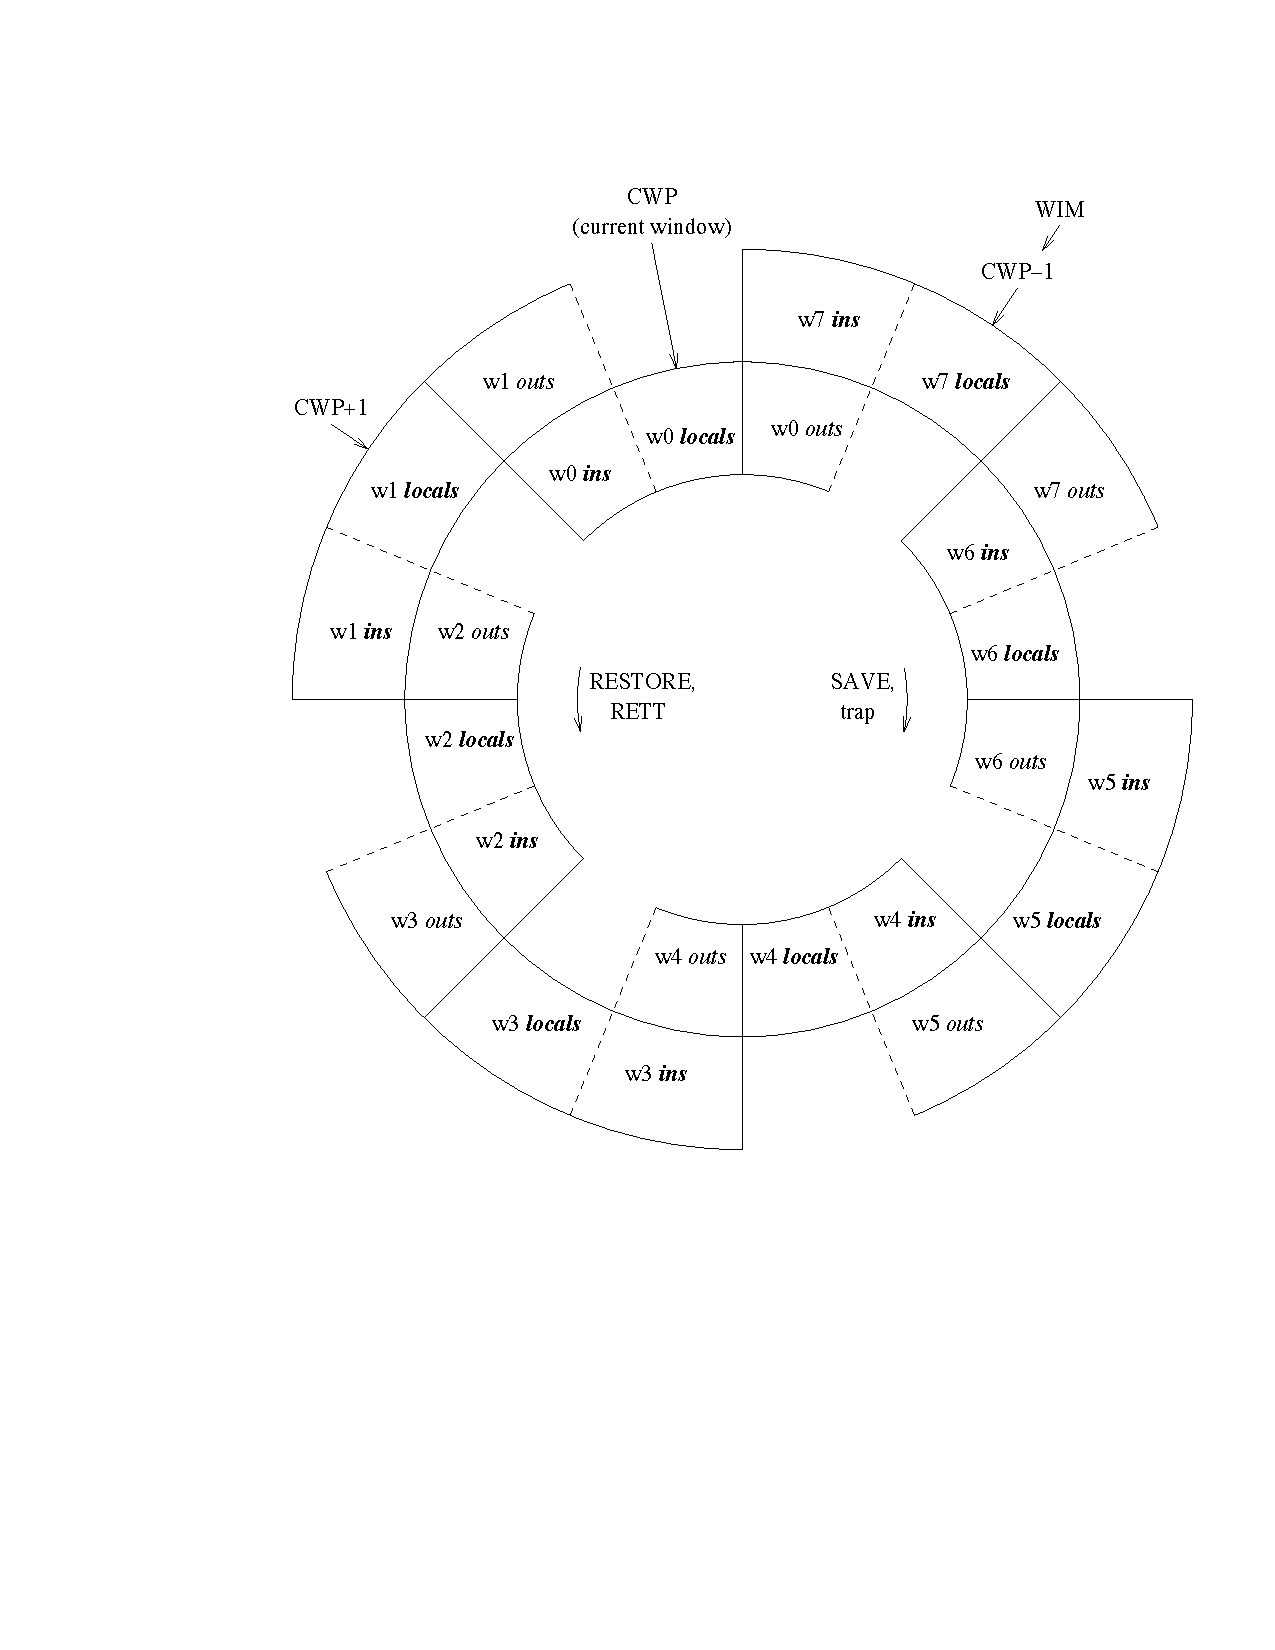
\includegraphics[width=8.7cm]{window}
	% 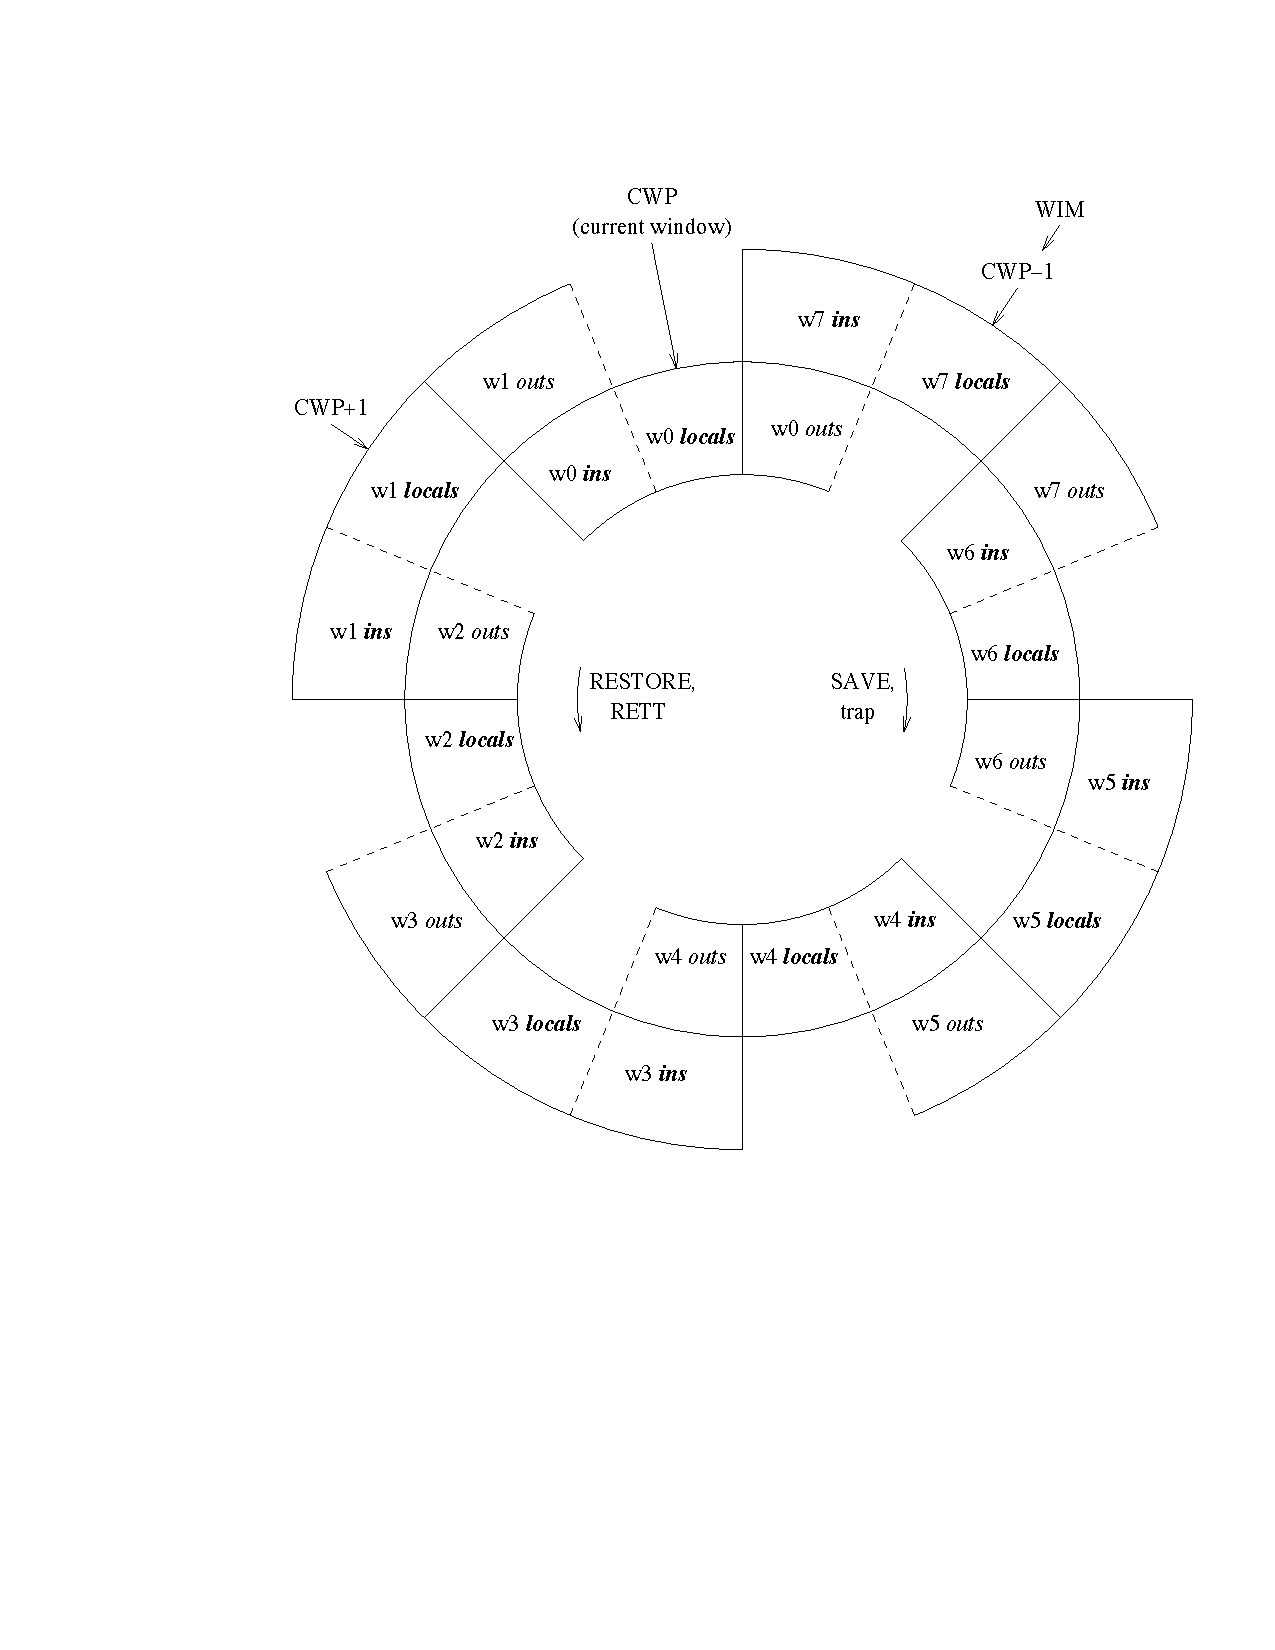
\includegraphics[width=58ex]{window}
	\caption{Register Windows (figure taken from \cite{sparc})}
	\label{fig:RegisterWindows}
\end{figure*}

The \inRN{} and \outRN{} registers of each window are shared
with its adjacent windows for parameter passing.
For example, the \inRN{} registers of the $\text{w}_0$
is the \outRN{} registers of the $\text{w}_1$,
and the \outRN{} registers of the $\text{w}_0$
is the \inRN{} registers of the $\text{w}_7$.
This explains
why we need only $2\times N$ groups of registers for
$N$ windows, while each window consisting of
three groups (\outRN{}, \localRN{} and \inRN{}).

To save the context, the $\csave$ instruction
rotates the window by decrementing the $\regcwp$ pointer
(modulo $N$).
So $\text{w}_7$ becomes the current window. The \outRN{}
registers of $\text{w}_0$ becomes
the \inRN{} registers of $\text{w}_7$.
The \inRN{} and \localRN{} registers of $\text{w}_0$
become inaccessible.
This is like pushing them
onto the circular stack.
The $\crestore$ instruction does the inverse, which is like
a stack pop.

The $\regwim$ register is used as a bit vector to record the
end of the stack. Each bit in $\regwim$ corresponds to a
register window. The bit corresponding to the last available
window is set to 1, which means {\em invalid}. All other bits
are 0 ({\em i.e. valid}).
%Given a window pointer $\cwp$ in $\regcwp$,
When executing $\csave$ (and $\crestore$), we need to ensure
the next window is valid, in order to avoid the overflow
of register window because of the limitation of the number
of windows. We use the assertion $\winvalid(\cwp, \RFile)$ defined
in Fig.~\ref{fig:save and restore} to say the
window pointed to by $\cwp$ is valid, given the value of
$\regwim$ in $\RFile$.
%$$
%\winvalid(\cwp, \RFile) \ \define \ 2^{\cwp}  \& \RFile(\regwim) = 0
%$$
%where $\&$ represents bitwise AND.

We use the frame list $\Wstack$ to model the circular stack consisting
of register windows. As defined in Fig.~\ref{fig:Register File and Frame List},
a frame is an array of 8 words, modeling a group of 8 registers.
$\Wstack$ consists of a sequence of frames
corresponding to all the
register windows except the \outRN{}, \localRN{} and \inRN{}
registers in the current window. Then $\csave$ saves the
\localRN{} and \inRN{} registers onto the head of $\Wstack$
and loads the two groups of register at the {\em tail} of $\Wstack$
to the \localRN{} and \outRN{} registers (and the original
\outRN{} registers becomes the \inRN{} group). The $\crestore$
instruction does the inverse. The operations are defined formally
in Fig.~\ref{fig:save and restore}.
Here, we use `` $\stCons$ " for
adding an element at the head of a list, and use `` $\lstApp{}$ "
for appending an element at the tail of a list.
\begin{figure*}[!t]
    \[
     \begin{array}{l}
     \outRN \ \define \  [\reg{8}, \dots, \reg{15}]
     \qquad
     \localRN \ \define \  [\reg{16}, \dots, \reg{23}] %
      \qquad
     \inRN \ \define \  [\reg{24}, \dots, \reg{31}]
     \\
     \\[-9pt]
     \RFile([\reg{i}, \dots, \reg{i+k}]) \ \define\
     [\RFile(\reg{i}), \dots, \RFile(\reg{i+k})]
     \\
     \\[-9pt]
     %
     \Rupd{\reg{i}, \dots, \reg{i+7}}{\fm} \ \define \
			R\{ \reg{i} \rightsquigarrow \val_0 \}
				\dots \{ \reg{i+7} \rightsquigarrow \val_7 \}
			\qquad
			\text{where }\ \ \fm = [\val_0, \dots, \val_7]
			% \\
            % \hspace*{28ex}\text{where }\ \ \fm = [\val_0, \dots, \val_7]
     \\
     \\ %[-8pt]
     %
     %\qquad \Rlocal \ \define\ [\RFile(\reg{8}), \dots, \RFile(\reg{15})] \\

        \begin{array}{lcl}
            \winvalid(\cwp, \RFile) & \define & 2^{\cwp}
											\,\bitAND\, \RFile(\regwim) = 0								
			\\
             & & \ \ \ \mbox{where $\bitAND$ is the bitwise AND operation.}
            \\
            \\[-9pt]
		    \precwp(\cwp) & \define & (\cwp + N - 1) \modOP N
            %\\
		    %\\[-8pt]
            \qquad\quad
		    \postcwp(\cwp) \ \define \ (\cwp + 1) \modOP N
        \end{array}
            \\
		    \\ %[-8pt]
            %
        \begin{array}{lcl}
            \decwin(\RFile, \Wstack) & \define &
            \left\{
            \begin{array}{ll}
                (\RFile', \Wstack')
                & \quad \textit{if }
                             \cwp' = \precwp(\RFile(\regcwp)),
                             \winvalid(\cwp', \RFile), \\
                & \quad \ \ \
                             \Wstack = \Wstack'' \lstApp \fm_1 \lstApp \fm_2, \
                              \Wstack' = \RFile(\localRN)
                                          \stCons\RFile(\inRN)\stCons\Wstack'',\\
                & \quad \ \ \ \RFile'' =
                \RFile\{\inRN\rightsquigarrow \RFile(\outRN),
                        \localRN\rightsquigarrow \fm_2,
                        \outRN \rightsquigarrow \fm_1\},
                \\
                 & \quad \ \ \
                            \RFile' = \fsubst{\RFile''}\regcwp{\cwp'},
                 \\
                 %
                \perp &\quad \textit{if }
                                  \lnot\winvalid(\precwp(R(\regcwp)), \RFile)
            \end{array}
            \right. \\
%            & & \where \ \ Q = (R, F)
            \\[-5pt]

            \incwin(\RFile, \Wstack) & \define &
            \left\{
            \begin{array}{ll}
                (\RFile', \Wstack')
                & \quad \textit{if }
                             \cwp' = \postcwp(\RFile(\regcwp)),
                             \winvalid(\cwp', \RFile), \\
                & \quad \ \ \
                             \Wstack = \fm_1 \stCons \fm_2 \stCons \Wstack''  , \
                              \Wstack' = \Wstack''\lstApp \RFile(\outRN)
                                                  \lstApp \RFile(\localRN), \\
                                          %\stCons\RFile(\inRN)\stCons\Wstack''\\
                & \quad \ \ \ \RFile'' =
                \RFile\{\inRN\rightsquigarrow \fm_2,
                        \localRN\rightsquigarrow \fm_1,
                        \outRN \rightsquigarrow \RFile(\inRN)\},
                \\
                 & \quad \ \ \
                            \RFile' = \fsubst{\RFile''}\regcwp{\cwp'},
                 \\
                 %
                \perp &\quad \textit{if }
                                  \lnot\winvalid(\postcwp(R(\regcwp)), \RFile)
            \end{array}
            \right.
        \end{array}
    \end{array}
    \]
    \caption{Auxiliary Definitions for Instruction \csave{} and \crestore}
    \label{fig:save and restore}
\end{figure*}

\paragraph{\textbf{The delay buffer.}}
The delay buffer $\DBuf$ is a sequence of delayed writes.
Because the  $\cwr$ instruction
does not update the target register immediately,
we put the write operation onto the delay buffer.
A delayed write is recorded as a triple consisting of
the remaining cycles $\tick$ to be delayed,
the target special register $\sr$ and the value
$\word$ to be written. 
Note that the value of a special register is restricted to 
only words, since the special registers are used to record the
state of processors, and it is impossible to
store memory addresses in them.
% Note that we restrict that
% the value of a special register can only be a word,
% because the special registers are used to record the
% state of processor, and it is impossible to
% store memory addresses in them.

\paragraph{\textbf{Instruction sequences.}}
%\indent \indent
We use an instruction sequence $\cblk$ to model
a basic block, \ie{} a sequence of commands ending
with a control transfer.
As defined in Fig.~\ref{fig:Machine States and Language for SPARC Code},
we require that a delayed control-transfer instruction
must be followed by  a simple instruction $\simplins$,
because the actual control-transfer occurs after
the execution of $\simplins$.
The end of each instruction sequence can only be
$\jmp$ or $\retl$  followed by a simple
instruction $\simplins$.
Note that we do not view the $\call$ instruction
as the end of a basic block, since the callee is
expected to return, following our direct-style
semantics for function calls.
We define $\code[\lab{}]$ to extract
an instruction sequence starting
from $\lab{}$ in $\code$ below.
\[
	\small
	C[\lab{}] =
	\left\{
		\begin{array}{ll}
			\simplins; \cblk &
			\quad \ \ \code(\lab{}) = \simplins \;
				\text{and} \; \code[\lab{}+4] = \cblk \\
			
			\\[-8pt]
			
			\comm; \simplins &
			\quad \ \
				\comm = \code(\lab{}) \; \text{and} \;
				\comm = \jmp \; \aexp \; \text{or} \; \retl
			\\ & \quad \ \ \text{and} \; C(\lab{}+4) = \simplins \\
			
			\\[-8pt]
			
			\comm; \simplins; \cblk &
			\quad \ \ \comm = \code(\lab{}) \;
			\text{and} \; c = \call \; \lab{} \; \text{or} \; \be \; \lab{} \\
			& \quad \ \ \text{and} \;
				\code(\lab{}+4) = \simplins \; \text{and} \;
				\code[\lab{}+8] = \cblk \\
			
			\\[-8pt]
			
			\undef & \quad \ \ \text{otherwise}
		\end{array}
	\right.
\]

\subsection{Operational Semantics}
\label{subsec : Operational Semantics}

The operational semantics is taken from
\etal{Wang}~\cite{sparc-formalization},
but we use a block-based memory model and
omit features like interrupts and traps.
We show the selected rules in Fig.~\ref{Selected Operational Semantics}.
\begin{figure*}
	\centering
	\subfigure[Program Transition]
	{
		\begin{minipage}[b]{1\textwidth}
		% \small
		\scriptsize
		\[
			\infer
			{
				\LGlobTrans
					{(\code, (\mem, (\RFile, \Wstack), \DBuf), \pc, \npc)}
					{ \ \ }
					{(\code, (\mem', (\RFile'', \Wstack'), \DBuf''), \pc', \npc')}
				% \ptrans{((M, (R, F), D), \pc, \npc)}
				% 	{((M', (R'', F'), D''), \pc', \npc')}
			}
			{
				\begin{array}{l}
					\Dstep{(R, D)}{(R', D')} \\
					\cttrans{((M, (R', F), D'), \pc, \npc)}
						{((M', (R'', F'), D''), \pc', \npc')}
				\end{array}
			}
		\]
		\vspace{0.05cm}
		\end{minipage}
	}
	
	\subfigure[Control Transfer Instruction Transition]
	{	
		\begin{minipage}[b]{1\textwidth}
		% \small
		\scriptsize
        \[
            \infer
            {
                \cttrans{((M, (R, F), D), \pc, \npc)}
                    {((M', (R', F'), D'), \npc, \npc+4)}
            }
            {
                \code(\pc) = \simplins \quad \quad
                    \swtrans{(M, (R, F), D)}{\; \; \simplins \; \;}{(M', (R', F'), D')}
            }
        \]

		\[
			\infer
			{
				\cttrans{((M, (R, F), D), \pc, \npc)}
					{((M, (R, F), D), \npc, \lab{})}
			}
			{
				C(\pc) = \jmp \; \aexp \quad \; \;
				\eval{\aexp} = \lab{}
			}
		\]
		
		\[
			\infer
			{
				\cttrans{((M, (R, F), D), \pc, \npc)}
				{
					((M, (R\{\reg{15} \rightsquigarrow \pc\}, F), D), \text{npc}, \lab{})
				}
			}
			{
				C(\pc) = \call \; \lab{} \quad \; \;
					\reg{15} \in \text{dom}(R)
			}			
		\]
		
		\[
			\infer
			{
				\cttrans{((M, (R, F), D), \pc, \npc)}
				{
					((M, (R, F), D), \npc, \lab{}\!+\!8)
				}
			}
			{
				C(\pc) = \retl \quad R(\reg{15}) = \lab{}
			}
		\]

		\[\!\!\!\!\!\!\!
			\infer
			{
				\cttrans{((\mem, (\RFile, \Wstack), \DBuf), \pc, \npc)}
					{((\mem, (\RFile, \Wstack), \DBuf), \npc, \lab{})}
			}
			{
				\code(\pc) = \be \ \lab{} \quad
				\RFile(\regz) \neq 0 \quad      
				%\RFile(\regz) = \word \quad
				%\word \neq 0
			} \qquad
			\infer
			{\cttrans{((\mem, (\RFile, \Wstack), \DBuf), \pc, \npc)}
				{((\mem, (\RFile, \Wstack), \DBuf), \npc, \npc\!+\!4)}}
			{
				\code(\pc) = \be \ \lab{} \quad
				\RFile(\regz) = 0
			}
		\]
		\vspace{0.05cm}
		\end{minipage}
	}
	
	\subfigure[Save, Restore and Wr instruction Transition]
	{
		\begin{minipage}[b]{1\textwidth}
			% \small
			\scriptsize
			\begin{minipage}{0.48\textwidth}
			\[
				\infer
				{
					\swtrans{(M, (R, F), D)}{\; \; \simplins \; \;}
						{(M', (R', F), D)}
				}
				{
					\itrans{(M, R)}{\simplins}{(M', R')}
				}
			\]
			\end{minipage}
			\begin{minipage}{0.48\textwidth}
				\[
					\infer
					{
						\swtrans{(M, (R, F), D)}
						{\cwr \; \reg{s} \; \oexp \; \sr}{(M, (R, F), D')}
					}
					{
						\begin{array}{l}
							R(\reg{s}) = \word_1 \quad \; \;
							{\llbracket \oexp \rrbracket}_R = \word_2 \quad \; \;
							w = \word_1 \!\xorOP\! \word_2 \\
							\sr \in \text{dom}(R) \quad \; \; D' = \textbf{set\_delay}(\sr, w, D)
						\end{array}
					}
				\]
			\end{minipage}

            \centering
            \vspace{0.3cm}
            \begin{minipage}{1\textwidth}
                \infer
                {
                    \swtrans{(\Mem, (\RFile, \Wstack), \DBuf)}
                    {\csave \; \reg{s} \; \oexp \; \reg{d}}
                    {(\Mem, (\RFile\{ \reg{d} \rightsquigarrow \val' \}, \Wstack'), \DBuf)}
                }
                {
					\decwin{(\RFile, \Wstack)} =
						(\RFile', \Wstack') \quad
                    \eval{\oexp} = \val
					\quad
					\val' = \RFile(\reg{s})\!+\!\val
                    % \RFile'' =
                    %   \fsubst{\RFile'}{\reg{d}}{\RFile(\reg{s}) \!+\! \val}
                }
                \vspace{0.3cm}
                \infer
                {
                    \swtrans{(\Mem, (\RFile, \Wstack), \DBuf)}
                    {\crestore \; \reg{s} \; \oexp \; \reg{d}}
                    {(\Mem, (\RFile\{ \reg{s} \rightsquigarrow \val' \}, \Wstack'), \DBuf)}
                }
                {
                    \incwin{(\RFile, \Wstack)} = (\RFile', \Wstack') \quad
                    \eval{\oexp} = \val
					\quad
					\val' = \RFile(\reg{s})\!+\!\val
                    % \RFile'' =
                    %   \fsubst{\RFile'}{\reg{d}}{\RFile(\reg{s}) \!+\! \val}
                    %R'' = R'\{ \reg{d} \rightsquigarrow \eval{\reg{s}} + \word \}
                }
            \end{minipage}
			
			\vspace{0.3cm}
		\end{minipage}
	}
	
	\subfigure[Simple Instruction Transition]
	{
		\begin{minipage}[b]{1\linewidth}
			% \small
			\scriptsize
			\begin{minipage}{0.5\linewidth}
				\[
					\infer
					{
						\itrans{(M, R)}{\rd \; \sr \; \reg{d}}
							{(M, R\{ \reg{d} \rightsquigarrow \word \})}
					}
					{
						R(\sr) = \word \quad \ \ \reg{d} \in \dom(R)
					}
				\]
			\end{minipage}
			\begin{minipage}{0.5\linewidth}
				\[
					\infer
					{
						\itrans{(M, R)}{\cadd \; \reg{s} \; \oexp \; \reg{d}}
						{
							(M, R\{\reg{d}
                                %  \rightsquigarrow \val_1\!+\!\val_2\})	
								\rightsquigarrow \val\})
						}
					}
					{
						R(\reg{s}) = \val_1 \quad
						{\llbracket \oexp \rrbracket}_R = \val_2 \quad
						\val = \val_1\!+\!\val_2 \quad
						\reg{d} \in \text{dom}(R)
					}
				\]
			\end{minipage}
			
			\vspace{0.2cm}
			\centering
			\begin{minipage}{1\textwidth}
				\[
					\infer
					{
						\itrans{(M, R)}{\ld \; \aexp \; \reg{d}}
						{(M, R\{\reg{d} \rightsquigarrow \val'\})}
					}
					{
						{\llbracket \aexp \rrbracket}_R = \loc \quad
						%\textbf{word\_align}(w) \quad
                        M(\loc) = \val' \quad
						\reg{d} \in \text{dom}(R)
					}
				\]
			\end{minipage}
			\vspace{0.3cm}
		\end{minipage}	
	}

	\subfigure[Expression Semantics]
	{
		\begin{minipage}[b]{1\linewidth}
			% \small
			\scriptsize
            $$
            \begin{array}{ll}
                \begin{array}{lcl}
                    \evalR{\oexp}{R} & \define &
                    \left\{
                        \begin{array}{ll}
                            R(r) &\quad \cif \ \oexp = r \\
                            \\[-8pt]
                            w &\quad \cif \ \oexp = \word, \\
                            & \quad \quad -4096 \leq \word \leq 4095 \\
                            \\[-8pt]
                            \perp &\quad \otherwise
                        \end{array}
                    \right.
                \end{array} & \quad
                \begin{array}{lcl}
                    \evalR{\aexp}{R} & \define &
                    \left\{
                        \begin{array}{ll}
                            \evalR{\oexp}{R} &\quad \cif \ \aexp = \oexp \\
                            \\[-8pt]

                            \val_1 \!+\! \val_2
                              &\quad \cif \ \aexp = \regr \!+\! \oexp,\
                              R(\regr) \!=\! \val_1 \\
                            & \quad \quad \tand \ \evalR{\oexp}{R} = \val_2 \\

                            \\[-8pt]
                            \perp &\quad \otherwise
                        \end{array}
                    \right.
                \end{array}
            \end{array}
            $$
			\vspace{0.3cm}
		\end{minipage}	
	}
	\caption{Selected operational semantics rules
		(taken from~\cite{sparc-formalization})}
	\label{Selected Operational Semantics}
\end{figure*}
The program transition relation
$\LGlobTrans{(\code, \state, \pc, \npc)}
	{ \ \, }
	{(\code, \state', \pc', \npc')}$
is defined
in Fig.~\ref{Selected Operational Semantics} (a).
Before the execution of the instruction pointed by
$\pc$, the delayed writes
in $\DBuf$ with $0$ delay cycles are executed first.
The execution of the delayed writes are defined in the
form of $\Dstep{(\RFile, \DBuf)}{(\RFile', \DBuf')}$ below:

{\small
$$
\begin{array}{c}
\!\!
\infer
{\Dstep{(\RFile, \nil)}{(\RFile,\nil)}}
{}
\quad \ \
%
% \qquad\qquad
%
\infer
{\Dstep{(\RFile, (\tick\!+\!1, \sr, \word)\dbCons\DBuf)}
       {(\RFile', (\tick, \sr, \word)\dbCons\DBuf')}}
{\Dstep{(\RFile, \DBuf)}{(\RFile', \DBuf')}}
\\
\\
\infer
{\Dstep{(\RFile, (0, \sr, \word)\dbCons\DBuf)}{(\fsubst{\RFile'}\sr\word, \DBuf')}}
{\Dstep{(\RFile, \DBuf)}{(\RFile', \DBuf')}
\qquad \sr\in\dom(\RFile)
}
%
% \qquad\qquad
\\
\\
%
\infer
{\Dstep{(\RFile, (0, \sr, \word)\dbCons\DBuf)}{(\RFile', \DBuf')}}
{\Dstep{(\RFile, \DBuf)}{(\RFile', \DBuf')}
 \qquad \sr\not\in\dom(\RFile)
}
\end{array}
$$
}

Note that the write of $\sr$ has no effect if $\sr$ is not
in the domain of $\RFile$. Since $\RFile$ is defined as a partial
map, we can prove the following lemma.
\begin{lemma}
	\label{lemma:RFileSplitExDelay}
	{\em $\Dstep{(\RFile, \DBuf)}{(\RFile', \DBuf')}$}
    and {\em $\RFile = \RFile_1 \uplus \RFile_2$},
    if and only if
    there exists {\em $\RFile_1'$} and {\em $\RFile_2'$}, such that
    {\em $\Dstep{(\RFile_1, \DBuf)}{(\RFile_1', \DBuf')}$, $\Dstep{(\RFile_2, \DBuf)}{(\RFile_2', \DBuf')}$},
    and {\em $\RFile' = \RFile_1' \uplus \RFile_2'$}.
\end{lemma}
Here the disjoint union $\RFile_1 \uplus \RFile_2$ represents the union of
$\RFile_1$ and $\RFile_2$ if they have disjoint domains, and undefined
otherwise. This lemma is important to give sound semantics
to delay buffer related assertions, as discussed in
Sec.~\ref{sec:logic}.

%Although this would never happen
%at runtime, this feature is useful for giving sound semantics
%to delay buffer related assertions, as shown in Sec.~\ref{sec:logic}.

%We define the operation semantics of \sparc{} with multiply layers.
%We just select a part of transition rules
%in Fig. \ref{Selected Operational Semantics}
%to give readers a whole recognition for \sparc{} program execution
%because of the space limitation.
%As shown in Fig. \ref{Selected Operational Semantics},
%we define the operational semantics with four layers.
%As for the first layer Program Transition,
%we can see that
%a step of \sparc{} program transition can be split into two steps.
%The state transition ``$\Dstep{}{}$" checks each element in delay list,
%remove the delay items whose delay cycles are 0
%and write the value recorded in them to specific special register.
%Second, the instruction that \pc{} points executes.
%We define the state transition caused by delay list simply as following.
%We can find that if a special register $\sr$ recorded in $\DBuf$ isn't
%in the domain of $\RFile$. It will not make any changes for $\RFile$.

%\[
%	\small
%	\begin{array}{rcl}
%		\exedelay(R, D) & \define &
%		\left\{
%			\begin{array}{ll}
%				(R, D) & \quad  D = \nil \\
%				
%				\\[-8pt]
%				
%				(R'\{\sr \rightsquigarrow w\}, D'') & \quad D = (0, \sr, w) :: D', \\
%				& \quad \ \ (R', D'') = \exedelay(R, D') \\
%				
%				\\[-8pt]
%				
%				(R', (n-1, \sr, w) :: D'') & \quad D = (n, \sr, w) :: D', n > 0, \\
%				& \quad \ \ (R', D'') = \exedelay(R, D')
%			\end{array}
%		\right.
%	\end{array}
%\]

The transition steps for individual instructions are classified into
three categories: the control transfer steps
($\ccttrans{\notCare}{\notCare}{\notCare}$),
the steps for
$\csave$, $\crestore$ and $\cwr$ instructions
($\swtrans{\notCare}{\ \notCare\ }{\notCare}$),
and the steps
for other simple instructions
($\itrans{\notCare}{\ \notCare\ }{\notCare}$). The
corresponding step transition relations are defined inductively
in Fig.~\ref{Selected Operational Semantics} (b), (c) and (d)
respectively.

Note that, after the control-transfer instructions, $\pc$ is set
to $\npc$ and $\npc$ contains the target code pointer. This explains
the one cycle delay for the control transfer.
The $\call$ instruction saves $\pc$ into the register $\RAreg$,
while $\retl$ uses $\RAreg \!+\! 8$ as the
return address (which is the address for the second instruction
following the $\call$).
The conditional branch $\be{} \ \lab{}$ jumps to $\lab{}$ 
(after one-cycle delay) if 
the value in the register $\regz$ is {\em not} 0.
%justifies whether
%the branch is taken according to the value of $\regz$.}
Evaluation of
expressions $\aexp$ and $\oexp$ are defined
% $\evalR\aexp\RFile$
% and
% $\evalR\oexp\RFile$
in Fig.~\ref{Selected Operational Semantics} (e).
Here, we define the sum of two values $\val_1$
and $\val_2$ below. The result of $\val_1\!+\!\val_2$
is legal, if both of the $\val_1$ and $\val_2$
are words (Int32), or $\val_1$ is an address and
$\val_2$ is an offset. The offset is a word,
which acts as an immediate value in the
calculation of address.
% This is explain why the
% immediate value in our work is a word, because
% immediate value usually acts as an offset, which
% is a word, in the calculation of address.
\[
	\small
	\val_1 + \val_2 \ \define \
	\left\{
		\begin{array}{ll}
			\word_1 + \word_2 & \quad \cif \
				\val_1 = \word_1, \text{ and }
				\val_2 = \word_2 \\
			\\[-8pt]
			(\block, \word_1 + \word_2) & \quad
				\cif \
				\val_1 = (\block, \word_1),
				\text{ and }
				\val_2 = \word_2 \\
			\\[-8pt]
			\perp & \quad \otherwise
		\end{array}
	\right.
\]

The $\cwr$ wants to save the bitwise exclusive OR of
the operands into the special register $\sr$, but
it puts the write into the delay buffer $\DBuf$
instead of updating $\RFile$ immediately.
The operation $\setdelay(\sr, \word, \DBuf)$
is defined below:
\[
	\begin{array}{l}
		\setdelay(\sr, \word, D) \define (X, \sr, \word)
		\dbCons \DBuf \\
	\end{array}
\]
where $X$ ($0 \leq X \leq 3$) is a
predefined system parameter for the delay cycle.
% Note that
% as we have explained before, special register is used
% to record the state of processors, so we do not permit saving
% memory address in it.
%whose specific value is implementation dependently.

The $\csave$ and $\crestore$ instructions rotate
the register windows and update the register file.
Their operations over $\Wstack$ and $\RFile$
are defined in Fig.~\ref{fig:save and restore}.

%Instruction $\csave$, $\crestore$ and $\cwr$
%are different with the other simple instructions
%because they may change the state of frame list and delay list.
%And we present their transition in the third layer.
%The rule for instruction $\cwr$ tells us
%that the \sparc{} set the write operation in delay list
%instead of updating the value of target special register $\sr$ immediately.
%The operation of $\setdelay(\sr, w, D)$ is defined as following,
%where $X$ ($0 \leq X \leq 3$) is the delay cycle
%whose specific value is implementation dependently :
%\[
%	\small
%	\begin{array}{l}
%		\setdelay(\sr, w, D) \define (X, \sr, w) :: D \\
%	\end{array}
%\]
%
%
%\indent
%The execution of instruction \csave{} and \crestore{} will cause the
%window rotation, so that will change the state of Frame List $F$.
%The operation $\decwin{(R, F)}$ describe that, if previous window is valid,
%we will do a right rotation for register windows by $\rightwin(R, F)$.
%As for instruction \crestore{}, it will change the register window by
%$\incwin{(R, F)}$, which will do a left rotation by $\leftwin(R, F)$ for register window.
%The auxiliary definitions for operational semantics of \csave{} and \crestore{}
%are shown in Fig. \ref{fig:save and restore}.
%
%\indent
%The last layer is designed for some simple instructions,
%whose executions only touch memory and register file.

  \section{Program Logic}
\label{sec:logic}

%\indent
In this section,
we introduce the assertion language
and program logic designed for \sparc{} program.
%We will elaborate how our logic handles the features of \sparc{} in detail.
%Finally, we will present our semantic approach for establishing soundness.

\subsection{Assertions}
\label{subsec:assertions}

\begin{center}
	$
		\begin{array}{rrcl}
			\textit{(Asrt)} & \astP, \astQ & \define & 
			\aemp \sepline
			\msto{l}{\val} \sepline
			\regst{\regN}{\val} \sepline
			\dlyregst{t}{\sr}{\word} \sepline 
			\asrttm{p} \\
			& & \ \ \ | &
			\frmst{\cwp}{F} \sepline
			\astP \wedge \astQ \sepline
			\astP \vee \, \astQ \sepline
			\astP \sepstar \astQ \\
			& & \ \ \ | &
			\aexp \addrEq \val \sepline
			\oexp = \val \sepline
			\forall x. \, \astP \sepline
			\exists x. \, \astQ \sepline
            \dots 
		\end{array}
	$
	\figurecaption{Syntax of Assertions}
	\label{fig:Syntax of Assertions}
	\vspace{-0.5em}
\end{center}

% \begin{figure*}[!t]
% 	\centering
% 	\small
% 	\vspace{-0.5em}
% 	\small
% 	$
% 		\begin{array}{rrcl}
%             \textit{(Asrt)} & \astP, q & \define &
%             \aemp \sepline
% 			\msto{l}{\val} \sepline
% 			\regst{\regN}{\val} \sepline
% 			\dlyregst{t}{\sr}{\word} \sepline

% 			\asrttm{p} \sepline
%             \frmst{\cwp}{F} \\ %\sepline \\
%             & &\ \,\sepline &
% 			%\apure{p} \sepline
% 			\astP \wedge \astQ \sepline
% 			\astP \vee \, \astQ \sepline
% 			\astP \sepstar \astQ \sepline
% 			\aexp \addrEq \val \sepline
% 			\oexp = \val \sepline
% 			\forall x. \, \astP \sepline
% 			\exists x. \, \astQ \sepline
%             \dots
% 		\end{array}
% 	$
% 	\caption{Syntax of Assertions}
% 	\label{fig:Syntax of Assertions}
% 	\vspace{-0.5em}
% \end{figure*}

\begin{figure*}[!t]
	\centering
	\vspace{-0.5em}
	$
		\begin{array}{l}
			\begin{array}{lcl}
				\asrtmodel{\state}{\aemp} & \define & S.M = \emptyset \, \wedge \, S.Q.R = \emptyset \\
				
				\asrtmodel{\state}{l \mapsto \val} & \define & 
					S.M = \{l \rightsquigarrow \val\} \, \wedge \,
                S.Q.R = \emptyset \\
				
				\asrtmodel{\state}{\regst{\regN}{\val}} & \define &
				S.Q.R = \{\regN \rightsquigarrow \val\}
                \, \wedge \, \regN \notin \dom(\state.\DBuf)
                \, \wedge \, \state.\mem = \emptyset \\
				
				\asrtmodel{\state}{\dlyregst{t}{\sr}{\word}} & \define &
                    \exists k,\RFile',\DBuf'.\,
                    0 \le k \le t\!+\!1
                    \land
                    \DstepN{k}{(\RFile, \DBuf)}{(\RFile', \DBuf')}
                    \land
                    \\ & & \hspace*{16ex}
                    \left(
                      \asrtmodel{(\mem, (\RFile', F), \DBuf')}{\regst{\sr}{\word}}
                    \right)
                    \land \noDup\DBuf\sr
                  \\
                  & & \hspace*{16ex}
                  \text{where }\state = (\mem, (\RFile, \Wstack), \DBuf)
                  \\

				\asrtmodel{\state}{\nxtAst\astP} & \define &
				\exists \RFile', \DBuf'. \;
                \left(
                  \asrtmodel{(\mem, (\RFile', \Wstack), \DBuf')}\astP
                \right)
                \land
                %\exedelay(R', D') = (S.Q.R, S.D)
                \Dstep{(\RFile', \DBuf')}{(\RFile, \DBuf)}
                  \\
                  & & \hspace*{16ex}
                  \text{where }\state = (\mem, (\RFile, \Wstack), \DBuf)
                  \\
				
				\asrtmodel{\state}{\frmst{\cwp}{\Wstack}} & \define &
				\left(\state \models \regst{\regcwp}{\cwp}\right) \, \wedge
                \exists \Wstack'.\, \Wstack \lstApp\Wstack' = S.Q.F \\

                \asrtmodel{S}{\aexpeq{\aexp}{\val}} & \define &
                \evalR{\aexp}{S.Q.R} = \val \, \wedge \, \wordaligned{(\val)} \\

                \asrtmodel{S}{\oexpeq{\oexp}{\val}} & \define & \evalR{\oexp}{S.Q.R} = \val \\
				
				\asrtmodel{S}{p_1 * p_2} & \define &
				\exists S_1, S_2. \; S_1 \models p_1 \, \wedge \, S_2 \models p_2 \, \wedge \,

				S = S_1 \uplus S_2

			\end{array} \\
			
			\\[-5pt]
			
			\state_1 \!\uplus\! \state_2 \ \define \
			\left\{
				\begin{array}{ll}
					(\mem_1 \!\cup\! \mem_2, (\RFile_1 \!\cup\! \RFile_2, \Wstack), \DBuf)
                         &  \quad \textbf{if} \; \mem_1 \!\perp\! \mem_2
                                  \wedge  \RFile_1 \!\perp\! \RFile_2  \wedge   \\
					& \quad \quad  \state_1 \!=\! (\mem_1, (\RFile_1, \Wstack), \DBuf)
                                  \wedge \state_2 \!=\! (\mem_2, (\RFile_2, \Wstack), \DBuf) \\
					
					\\[-8pt]
					
					\undef & \quad \text{otherwise}
				\end{array}
			\right. \\
			
			\\[-5pt]
%			\DtoS\DBuf \ \define \
%			\left\{
%			\begin{array}{ll}
%				\{(n, \sr, \word)\} \cup \DtoS{\DBuf'}
%                    & \quad \textbf{if} \;
%                         \DBuf = (n, \sr, \word) \dbCons \DBuf' \\
%				
%				\\[-8pt]
%				
%				\emptyset & \quad \textbf{if} \; \DBuf = \nil
%			\end{array}
%			\right.
%            \\
%			
%			\\[-5pt]

			\dom(\DBuf) \ \define \
			\left\{
			\begin{array}{ll}
				\{\sr\} \cup \dom(\DBuf') & \quad \textbf{if} \;
                         \DBuf = (\tick, \sr, \word) \dbCons \DBuf' \\
				
				\\[-8pt]
				
				\emptyset & \quad \textbf{if} \; \DBuf = \nil
			\end{array}
			\right.
            \\
			
			\\[-5pt]
%
			\noDup\DBuf\sr \ \define \
			\left\{
			\begin{array}{ll}
				\sr\not\in\dom(\DBuf')
                    & \quad \textbf{if} \;
                         \DBuf = (\tick, \sr, \word) \dbCons \DBuf' \\
				
				\\[-8pt]
				
				\sr\neq\sr' \land \noDup{\DBuf'}\sr
                    & \quad \textbf{if} \;
                         \DBuf = (\tick, \sr', \word) \dbCons \DBuf' \\
				
				\\[-8pt]
				\textbf{True} & \quad \textbf{if} \; \DBuf = \nil
			\end{array}
			\right.
            \\
			
			\\[-5pt]

%			\noDup\DBuf\sr \ \define \
%             \forall n_1, n_2, \word_1, \word_2.
%             (n_1, \sr, \word_1) \!\in\! \DtoS\DBuf \land
%             (n_2, \sr, \word_2) \!\in\! \DtoS\DBuf
%             \Rightarrow
%             \\ \hspace*{55ex}
%             n_1 \!=\! n_2 \land \word_1 \!=\! \word_2
%%            \qquad
%%			\textbf{noDup} (\sr, lr) \ \define \
%%			\sr \notin lr \backslash \{\sr\}
%            \\
%			
%			\\[-5pt]
			
%			\substFld{S}{R', D'} \define (M, (R', F), D'),
%            \ \ \ \ \text{where } S = (M, (R, F), D)
%            \\
%            \\[-5pt]

            %\begin{array}{ll}
%                \begin{array}{lcl}
%                    \evalR{\oexp}{R} & \define &
%                    \left\{
%                        \begin{array}{ll}
%                            R(r) &\quad \cif \ \oexp = r \\
%                            \\[-8pt]
%                            w &\quad \cif \ \oexp = \word, \\
%                            & \quad \quad -4096 \leq \word \leq 4095 \\
%                            \\[-8pt]
%                            \perp &\quad \otherwise
%                        \end{array}
%                    \right.
%                \end{array} & \quad
%                \begin{array}{lcl}
%                    \evalR{\aexp}{R} & \define &
%                    \left\{
%                        \begin{array}{ll}
%                            \evalR{\oexp}{R} &\quad \cif \ \aexp = \oexp \\
%                            \\[-8pt]
%
%                            v_1 \!+\! v_2 &\quad \cif \ \aexp = r \!+\! \oexp,\
%                              R(r) \!=\! v_1 \\
%                            & \quad \quad \tand \ \evalR{\oexp}{R} = v_2 \\
%
%                            \\[-8pt]
%                            \perp &\quad \otherwise
%                        \end{array}
%                    \right.
%                \end{array}
%            \end{array}
		\end{array}
	$
	\caption{Semantics of Assertions}
	\label{fig:Semantics of Assertions}
	\vspace{-0.5em}
\end{figure*}

%\indent
We define syntax of assertions in Fig.~\ref{fig:Syntax of Assertions},
and their semantics in Fig.~\ref{fig:Semantics of Assertions}.
We extend separation logic assertions with specifications of
delay buffers and register windows. Registers are like
variables in separation logic, but are treated as resources.
The assertion $\aemp$ says
that the memory and the register file are both empty.
$\msto{\loc}{\val}$ specifies a singleton memory cell
with value $\val$ stored in the address $l$.
$\regst{\regN}{\val}$ says that
$\regN$ is the only register in the register file
and it contains the value $\val$. Also
$\regN$ is {\em not} in the delay buffer.
Separating conjunction $\astP \sepstar \astQ$ has the
standard semantics as in separation logic \cite{separationlogic}.
%there is only one cell in register file
%that maps the register name $\regN$ to value $\word$ and $\regN$ is not in delay list.


%Our assertion language is shown in Fig. \ref{fig:Syntax of Assertions}.
%And the semantics of some of them are presented
%in Fig. \ref{fig:Semantics of Assertions}.

%\indent
%Assertion emp says
%that the memory and register file are both empty.
%$\msto{l}{\word}$ specifies a singleton memory cell
%with value $\word$ stored in address $l$.
%$\regst{\regN}{\word}$ says that
%there is only one cell in register file
%that maps the register name $\regN$ to value $\word$ and $\regN$ is not in delay list.

%Delayed writes cause uncertainty of special registers $\sr$
%in $\RFile$.
The assertion $\dlyregst{\tick}{\sr}{\word}$ describes a delayed
write in the delay buffer $\DBuf$. It describes the
uncertainty of $\sr$'s value in $\RFile$, which is unknown
for now but will become $\word$ in up to $\tick\!+\!1$ cycles.
%It says the value of $\sr$ in the register file is unknown, but
%it will become $\word$ in up to $\tick\!+\!1$ cycles.
We use $\DstepN{k}{\notCare}{\notCare}$
to represent $k$-step execution of the delayed writes in $\DBuf$.
It also requires that there be
at most one delayed write for a specific special register $\sr$
in $\DBuf$ (\ie{} $\noDup{\sr}{\DBuf}$).
This prevents more than one delayed writes to
the same register within 4 instruction cycles, which practically
have no restrictions on programming.
By the semantics we have
$$
\regst{\sr}{\word} \,\Longrightarrow \dlyregst{\tick}{\sr}{\word}
\qquad
\dlyregst{\tick}{\sr}{\word} \,\Longrightarrow\,
\dlyregst{\tick\!+\!k}{\sr}{\word}
$$

The assertion $\nxtAst\astP$ allows us to reduce the uncertainty
by executing one step of the delayed writes.
It specifies states reachable after executing
one step of delayed writes from those states satisfying $\astP$.
Therefore we know:
$$
\nxtAst{(\dlyregst{0}{\sr}{\word})} \Longrightarrow 
\regst{\sr}{\word}
\quad \
\nxtAst{(\dlyregst{\tick\!+\!1}{\sr}{\word})} \Longrightarrow
\dlyregst{\tick}{\sr}{\word}
$$
Also it's easy to see that if $\astP$ syntactically
does not contain sub-terms in the form of $\dlyregst{\tick}{\sr}{\word}$,
then $(\nxtAst\astP) \,\Longleftrightarrow \,\astP$.

The following lemma shows $\nxtAst{(\notCare)}$ is distributive
over separating conjunction.
\begin{lemma} %\mbox{}
\label{lemma:dly-sep-split}
$
\nxtAst{(\astP * \astQ)} \,\Longleftrightarrow\, (\nxtAst\astP) * (\nxtAst\astQ)\,.
$
%\end{enumerate}
\end{lemma}
The lemma can be proved following Lemma~\ref{lemma:RFileSplitExDelay}.


We use $\frmst{\cwp}{\Wstack}$ to describe the pointer
$\regcwp$ of the current register window and the frame
list as a circular stack.
Note that $\Wstack$ is just a prefix of the frame list,
since usually we do not need to know contents of
the full list. Here we use $\Wstack \lstApp \Wstack'$ to
represent the concatenation of lists $\Wstack$ and $\Wstack'$.
Therefore we have
$
\frmst{\cwp}{\Wstack \lstApp \Wstack'} \,\Longrightarrow\,
\frmst{\cwp}{\Wstack}
$\,.


The assertions $\aexpeq{\aexp}{\val}$ and $\oexpeq{\oexp}{\val}$
describe the value of $\aexp$ and $\oexp$ respectively. They are
intuitionistic assertions. Since $\aexp$ is used as an address,
we also require it to be properly aligned on a 4-byte boundary. 
We define $\wordaligned{}$ to represent this restriction below. 
The result of the address expression $\aexp$ may be a word, if 
it's a pointer in code heap, or a memory address, if it's a location 
of memory. 
\[
	\wordaligned{(\val)} \define
	\exists \, \word, \block. \, 
	(\val = \word \, \lor \, \val = (\block, \word))
	\, \land \, \word\modOP{4} = 0 
	% \exists \, \word. \, 
	% (\val = \word \, \lor \, (\exists \, \block. \, \val = (\block, \word)))
	% \, \land \, \word\modOP{4} = 0 
\]

\subsection{Inference Rules}
\label{subsec:inference rules}
\newcommand{\tinybftext}[1]{\textbf{\scriptsize{#1}}}

%\begin{figure}[!t]
%	\centering
%	\subfigure[]
%	{
%		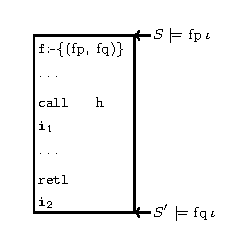
\includegraphics[width=35ex]{picture//funspec}
%		\label{fig:function specification}
%	}
%	\hspace{3em}
%	\subfigure[]
%	{
%		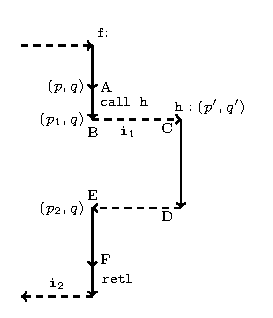
\includegraphics[width=38ex]{picture//CallReturnHandling}
%		\label{fig:call return handling}
%	}
%	\label{fig:Function Call/Return and Delayed-control-transfer Handling}
%	\caption{Function Call/Return and Delayed-control-transfer Handling}
%\end{figure}

%\indent
%We define a set of inference rules
%so that we can check \sparc{} code mechanized.
The code specification $\theta$ and code heap specification $\Psi$
are defined below:
\[
	\small
	\begin{array}{lccllccl}
		\text{(valList)} & \lgvl & \in & \text{list value} 
			& 
		\multicolumn{4}{l}
		{
			\quad
			\text{(pAsrt)} \ \
			\specpre,\specpost \ \in \ 
			\text{valList} \rightarrow Asrt
		}
		% \specpre,\specpost &
		% 			\in & \text{valList} \rightarrow Asrt 
		\\
		
		\text{(CdSpec)} & \Bspec & ::= & (\specpre, \specpost) 
			& \quad
		
		\text{(CdHpSpec)} & \Cspec & ::= & \{\lab{} \rightsquigarrow \Bspec\}^{*}
	\end{array}
\]

The code heap specification $\Psi$ maps the code labels
for basic blocks to their specifications $\theta$,
which is a pair of pre- and post-conditions.
Instead of using normal assertions, the pre- and
post-conditions are assertions parameterized over
a list of values $lgvl$. They play the role
of auxiliary variables --- Feeding the pre-
and the post-conditions with the same $lgvl$ allows
us to establish relationship of states specified
in the pre- and post-conditions.

Although we assign a $\theta$ to each basic block,
the post-condition does not specify the states reached at the end
of the block. Instead, it specifies the condition
that needs to be specified in the future when the
{\em current function} returns. This follows the idea
developed in SCAP~\cite{Feng06pldi}, but we use the
standard unary state assertion instead of the binary
state assertions used in SCAP, so that existing
proof techniques (such as Coq tactics) for standard
Hoare-triples can be applied to simplify the verification
process.

\begin{center}
	\vspace*{-2em}
	$$
	\begin{array}{l}
		\begin{array}{ll}
			- & \{(\text{fp}, \text{fq})\} \\
			& \cadd \quad \ireg{0}, \, \ireg{1}, \, \lreg{7} \\
			& \cadd \quad \lreg{7}, \, \ireg{2}, \, \lreg{7} \\
			& \retl \\
			& \nop
		\end{array} \\
		\\
		\begin{array}{lcl}
			\text{fp} & \define &
			\lambda \, \lv.\, 
			(\regst{\ireg{0}}{\lv[0]})
			* (\regst{\ireg{1}}{\lv[1]})
			* (\regst{\ireg{2}}{\lv[2]}) \\
			& &
			\hspace*{6ex} * \regst{\lreg{7}}{\notCare}
						  * (\regst{\reg{15}}{\lv[3]}) \\

			
			\\[-8pt]
			
			\text{fq} & \define & \lambda \, lv. \;
			(\regst{\ireg{0}}{\lv[0]})
			* (\regst{\ireg{1}}{\lv[1]})
			* (\regst{\ireg{2}}{\lv[2]}) \\
			& &
			\hspace*{6ex}
			* (\regst{\lreg{7}}{\lv[0] \!+\! \lv[1] \!+\! \lv[2]})
						  * (\regst{\reg{15}}{\lv[3]})
		\end{array}
	\end{array}
	$$
	\vspace*{-0.5em}
	\figurecaption{Example for Function Specification}
	\label{fig:functionSpec}
\end{center}

We give a simple example in Fig.~\ref{fig:functionSpec}
to show a specification for a function,
which simply
sums the values of the registers $\ireg{0}$, $\ireg{1}$ and $\ireg{2}$
and writes the result into the register $\lreg{7}$.
The specification $(\specpre,\specpost)$ says that, when
provided with the same $\lv$ as argument, the function
preserves the value of $\ireg{0}$, $\ireg{1}$ and $\ireg{2}$,
$\lreg{7}$ at the end contains the sum of $\ireg{0}$, $\ireg{1}$ and $\ireg{2}$, and the function also preserves the value of $\RAreg$,
which it uses as the return address.
To verify the function, we need to prove that it satisfies
$(\specpre\,\lv, \specpost\,\lv)$ for all $\lv$.


%In order to get connection between initial state and final state,
%we define a list of logical variables LogicVL
%as a parameter of code block's pre/postcondition.
%A predicate \specpre{} specifies the initial state,
%and the other predicate \specpost{} describe the state
%at the return point of the current function.
%Fig. \ref{fig:function specification}
%shows the meaning of our specification (\specpre{}, \specpost{}) for function f.
%The code specification $\Psi$ is defined as
%a finite mapping from code labels to code specifications.
%we give a simple example to introduce
%how to write a specification for a function implemented by \sparc{}
%in Fig. \ref{fig:functionSpec}.

%\paragraph{\textbf{Example of Function Specification.}}
%The function shown in Fig. \ref{fig:functionSpec}
%sums the values of registers $\ireg{0}$, $\ireg{1}$ and $\ireg{2}$ together
%and writes the result into register $\lreg{7}$.
%The specification of the function is presented by $(\specpre, \specpost)$.
%Here, we need to describe the state of register $\reg{15}$,
%which saves the label of occurring function call, in pre/postcondition.
%However, we don't have to know the concrete value of $\reg{15}$
%with the inspiration provided by SCAP.
%Both of pre/postcondition parameter a list of logic variables
%for getting connection between them.
%We will find that
%using a list of logic variables is essential in some situation
%for writing specification.
%For example,
%we can't describe the call point stored in register $\reg{15}$ equally
%between initial and final state,
%without the helping of the list of logic variables.
%The main role of list of logic variables is to
%describe the same logic variables used both in
%pre/postcondition.

\begin{figure*}[!thp]
	\subfigure
	{
		\begin{minipage}{1\linewidth}
			$\boxed{\vdash \code : \Psi}$ \quad \quad
			\textbf{(Well-Formed Code Heap)}
			\[
				\infer[\tinybftext{(CDHP)}]
				{
					%\Psi \vdash \code : \Psi'
					\vdash \code : \Psi
				}
				{
					\text{for all} \; \lab{} \in \dom(\Psi), \; \lgvl \, :
					\; \; \Psi(\lab{}) = (\specpre, \specpost) \quad \;
					\wfcblk{\specpre \; \lgvl}{\specpost \; \lgvl}{\lab{}}{C[\lab{}]}
				}
			\]
		\end{minipage}
	}
	
	\subfigure
	{
		\begin{minipage}{1\linewidth}
			$\boxed{\wfcblk{\astP}{\astQ}{\lab{}}{\cblk}}$ \quad \quad
			\textbf{(Well-Formed Instruction Sequences)}
%
			\[
				\infer[\tinybftext{(SEQ)}]
				{
					\wfcblk{\astP}{\astQ}{\lab{}}{\simplins; \, \cblk}
				}
				{
					\begin{array}{l}
						\wfins{\nxtAst{\astP}}{\simplins}{\astP'} \quad \; \;
						\wfcblk{\astP'}{\astQ}{\lab{}\!+\!4}{\cblk}
					\end{array}
				}
			\]
%
%
            \[
                \infer[\tinybftext{(JMP)}]
                {
                    \wfcblk{\astP}{\astQ}{\lab{}}{\jmp \; \aexp; \, \simplins}
                }
                {
                    \begin{array}{c}
                        \nxtAst{\astP}
                          \,\Rightarrow\, (\aexpeq{\aexp}{\lab{}'}) \quad
                        \lab{}' \in \dom(\Psi) \quad \Psi(\lab{}') = (\specpre, \specpost) \\
                        \wfins{\nxtAst{\nxtAst{\astP}}}{\simplins}{\astP'} \quad
%                        \exists \lgvl. \;
%                        (\astP' \,\Rightarrow\,
%                        \specpre \; \lgvl)
%                        \, \land \,
%                        (\specpost \; \lgvl \,\Rightarrow\, \astQ)
                        \exists \lgvl,\pr. \;
                        (\astP' \,\Rightarrow\,
                        \specpre \; \lgvl * \pr)
                        \, \land \,
                        (\specpost \; \lgvl * \pr \,\Rightarrow\, \astQ)
                    \end{array}
                }
            \]
%
			\[
				\infer[\tinybftext{(CALL)}]
				{
					\wfcblk{\astP}{\astQ}{\lab{}}{\call \; \lab{}'; \, \simplins; \, \cblk}
				}
				{
					\begin{array}{c}
						\lab{}' \in \dom(\Psi) \quad
						\Psi (\lab{}') = (\specpre, \specpost) \quad
						\wfcblk{\astP'}{\astQ}{\lab{}\!+\!8}{\cblk} \\
						\nxtAst{\astP} \,\Rightarrow\,
                             (\regst{\reg{15}}{\notCare})
                                 * \astP_1
						\quad
						\wfins{\asrttm{(\regst{\reg{15}}{\lab{}} * \astP_1)}}
						{\simplins}{\astP_2}  \\
						\exists  \lgvl, \pr. \;
						\supimpl{\astP_2}{\astP'}{\specpre \; \lgvl * \pr}{\specpost \; \lgvl * \pr} \, \wedge \,
						(\specpost \; \lgvl \Rightarrow \reg{15} \!=\! \lab{})
					\end{array}	
				}
			\]
%
%
%
			\[
				\infer[\tinybftext{(RETL)}]
				{
					\wfcblk{\astP}{\astQ}{\lab{}}{\retl; \, \simplins}
				}
				{
                    \nxtAst{\nxtAst{\astP}} \,\Rightarrow
                      (\regst\RAreg{\lab{}'}) * \astP_1
                      \quad
                    \wfins{\astP_1}{\simplins}{\astP_2}
                    \quad
					(\regst\RAreg{\lab{}'}) * \astP_2 \Rightarrow \astQ
				}
			\]
%			\[
%				\infer[\tinybftext{(RETL)}]
%				{
%					\wfcblk{\astP}{\astQ}{\lab{}}{\retl; \, \simplins}
%				}
%				{
%					\wfins{\nxtAst{\nxtAst{\astP}}}{\simplins}{\astP'}
%					\quad \; \;
%					\astP' \Rightarrow \astQ \quad \; \;
%                    \RAsta{\nxtAst{\nxtAst{\astP}}}{\astP'}
%				}
%			\]
%
%
%
%<<<<<<< .mine
%			\[
%				\infer[\tinybftext{(BE)}]
%				{
%					\wfcblk{\astP}{\astQ}{\lab{}}
%					{\be \; \lab{}'; \, \simplins; \, \cblk}
%				}
%				{
%					\begin{array}{l}
%						\lab{}' \in \dom(\Psi) \quad
%						\Psi (\lab{}') = (\specpre, \specpost) \quad
%						\wfcblk
%						{\asrttm{(p \, \wedge \, \regz = 0)}}{\astQ}
%						{\lab{}+4}{\simplins; \, \cblk} \\
%						\wfins{\asrttm{\asrttm{(\astP \wedge \regz \neq 0)}}}
%						{\simplins}{\astP'} \quad
%						\exists \; \lgvl. \;
%						\supimpl{\astP'}{\astQ}{\specpre \; \lgvl * \pr}{\specpost \; \lgvl * \pr}
%					\end{array}
%				}
%			\]
%%
%%
%%
%            \[
%                \infer[\tinybftext{(J)}]
%                {
%                    \wfcblk{\astP}{\astQ}{\lab{}}{\jmp \; \aexp; \, \simplins}
%                }
%                {
%                    \begin{array}{l}
%                        \nxtAst{\astP} \Rightarrow \aexpeq{\aexp}{\lab{}'} \quad
%                        \lab{}' \in \dom(\Psi) \quad \Psi(\lab{}') = (\specpre, \specpost) \\
%                        \wfins{\nxtAst{\nxtAst{\astP}}}{\simplins}{\astP'} \quad
%                        \exists \lgvl. \; (\astP' \Rightarrow \specpre \; \lgvl * \pr) \,
%                        \land \, (\specpost \; \lgvl * \pr \Rightarrow \astQ)
%                    \end{array}
%                }
%            \]
%			\vspace{0.01em}
%			\centering
%			\[
%				\infer[\tinybftext{(FRAME)}]
%				{
%					\wfcblk{\astP * \pr}{\astQ * \pr}{\lab{}}{\cblk}
%				}
%				{
%					\wfcblk{\astP}{\astQ}{\lab{}}{\cblk}
%				}
%			\]
%||||||| .r65
%			\[
%				\infer[\tinybftext{(BE)}]
%				{
%					\wfcblk{\astP}{\astQ}{\lab{}}
%					{\be \; \lab{}'; \, \simplins; \, \cblk}
%				}
%				{
%					\begin{array}{l}
%						\lab{}' \in \dom(\Psi) \quad
%						\Psi (\lab{}') = (\specpre, \specpost) \quad
%						\wfcblk
%						{\asrttm{(p \, \wedge \, \regz = 0)}}{\astQ}
%						{\lab{}+4}{\simplins; \, \cblk} \\
%						\wfins{\asrttm{\asrttm{(\astP \wedge \regz \neq 0)}}}
%						{\simplins}{\astP'} \quad
%						\exists \; \lgvl. \;
%						\supimpl{\astP'}{\astQ}{\specpre \; \lgvl * \pr}{\specpost \; \lgvl * \pr}
%					\end{array}
%				}
%			\]
%%
%%
%%
%            \[
%                \infer[\tinybftext{(J)}]
%                {
%                    \wfcblk{\astP}{\astQ}{\lab{}}{\jmp \; \aexp; \, \simplins}
%                }
%                {
%                    \begin{array}{l}
%                        \nxtAst{\astP} \Rightarrow \aexpeq{\aexp}{\lab{}'} \quad
%                        \lab{}' \in \dom(\Psi) \quad \Psi(\lab{}') = (\specpre, \specpost) \\
%                        \wfins{\nxtAst{\nxtAst{\astP}}}{\simplins}{\astP'} \quad
%                        \exists \lgvl. \; \astP' \Rightarrow \specpre \; \lgvl * \pr \,
%                        \land \, \specpost \; \lgvl * \pr \Rightarrow \astQ
%                    \end{array}
%                }
%            \]
%			\vspace{0.01em}
%			\centering
%			\[
%				\infer[\tinybftext{(FRAME)}]
%				{
%					\wfcblk{\astP * \pr}{\astQ * \pr}{\lab{}}{\cblk}
%				}
%				{
%					\wfcblk{\astP}{\astQ}{\lab{}}{\cblk}
%				}
%			\]
%=======
%			\[
%				\infer[\tinybftext{(BE)}]
%				{
%					\wfcblk{\astP}{\astQ}{\lab{}}
%					{\be \; \lab{}'; \, \simplins; \, \cblk}
%				}
%				{
%					\begin{array}{l}
%						\lab{}' \in \dom(\Psi) \quad
%						\Psi (\lab{}') = (\specpre, \specpost) \quad
%						\wfcblk
%						{\asrttm{(p \, \wedge \, \regz = 0)}}{\astQ}
%						{\lab{}+4}{\simplins; \, \cblk} \\
%						\wfins{\asrttm{\asrttm{(\astP \wedge \regz \neq 0)}}}
%						{\simplins}{\astP'} \quad
%						\exists \; \lgvl. \;
%						\supimpl{\astP'}{\astQ}{\specpre \; \lgvl * \pr}{\specpost \; \lgvl * \pr}
%					\end{array}
%				}
%			\]
%%
%%
%%
%			\vspace{0.01em}
%			\centering
%			\[
%				\infer[\tinybftext{(FRAME)}]
%				{
%					\wfcblk{\astP * \pr}{\astQ * \pr}{\lab{}}{\cblk}
%				}
%				{
%					\wfcblk{\astP}{\astQ}{\lab{}}{\cblk}
%				}
%			\]
%>>>>>>> .r66
		\end{minipage}
	}
	
	\subfigure
	{
		\begin{minipage}{1\linewidth}
			$\boxed{\wfins{p}{\simplins}{q}}$ \quad \quad
			\textbf{(Well-Formed Instructions)}
			
%			\hspace{-0.8cm}
%			\begin{minipage}{0.53\linewidth}
%				\[
%					\infer[\tinybftext{(LD)}]
%					{
%						\wfins{p}{\ld \; \aexp \; \reg{d}}
%						{\msto{l}{v} * \regst{\reg{s}}{v} * p_1}
%					}
%					{
%						p \Rightarrow \aexp =_{a} l \quad p \Rightarrow \msto{l}{v} * \regst{\reg{s}}{\_} * p_1
%					}
%				\]
%			\end{minipage}
%			\begin{minipage}{0.53\linewidth}
%				\[
%					\infer[\tinybftext{(ADD)}]
%					{
%						\wfins{p}{\cadd \; \reg{s} \; \oexp \; \reg{d}}
%						{(\regst{\reg{d}}{v_1 + v_2}) * p_1}
%					}
%					{
%						\begin{array}{l}
%							p \Rightarrow (\reg{s} = v_1 \wedge \oexp = v_2) \quad
%							p \Rightarrow \regst{\reg{d}}{\_} * p_1
%						\end{array}
%					}
%				\]
%			\end{minipage}
			\[
				\infer[\tinybftext{(WR)}]
				{
					\wfins{\regst{\sr}{\notCare} * p}{\cwr \; \reg{s} \; \oexp \; \sr}
					{(\dlyregst{3}{\sr}{(\word_1 \xorOP \word_2)} ) * p}
				}
				{
					\regst{\sr}{\notCare} * p \Rightarrow (\reg{s} = \word_1 \, \wedge \, \oexp = \word_2)
				}
			\]
            \[
                \infer[\tinybftext{(RD)}]
                {
                    \wfins{\regst{\sr}{\word} * \regst{\reg{d}}{\notCare}}{\rd \; \sr \; \reg{d}}
                    {\regst{\sr}{\word} * \regst{\reg{d}}{\word}}
                }
                {}
            \]
			%\centering
%
%
			\[\begin{array}{l}
				\infer[\tinybftext{(SAVE)}]
				{
					\wfins{(\regst{\regwim}{\word}) * p}
					{\csave \; \reg{s} \; \oexp \; \reg{d}}
					{(\regst{\regwim}{\word}) * 
					% (\regst{\reg{d}}{\val_1 \!+\! \val_2}) * p_2}
					(\regst{\reg{d}}{\val}) * p_2}
				}
				{
					\begin{array}{c}
						p \Rightarrow (\reg{s} = \val_1 \wedge \oexp = \val_2) \quad \; \;
						\cwp' = \precwp(\cwp) \quad \; \;
						\word \,\bitAND\, 2^{\cwp'} = 0 \quad \; \;
						\val = \val_1\!+\!\val_2 \\
						p \Rightarrow
                        %(\regst\regcwp\cwp) *
                        %\stackAst{\Wstack} *
						\left(\frmst{\cwp}{\Wstack \lstApp \, \notCare \, \lstApp \, \notCare}\right) *
						(\OutRegs{\fm_o}) *
                        (\LocalRegs{\fm_l}) *
                        (\InRegs{\fm_i})
                        * p_1 \\
						%\frmst{\cwp}{F \circ \fm_1 \circ \fm_2} *
						%\Regs{\fm_o}{\fm_l}{\fm_i} * p_1 \\
                        %
                        %(\regst\regcwp{\cwp'}) *
                        %\stackAst{\fm_l \stCons \fm_i \stCons \Wstack} *
						\left(\frmst{\cwp'}
                                    {\fm_l \stCons \fm_i \stCons \Wstack}\right) *
						\Regs{\notCare}{\notCare}{\fm_o} * p_1
						\Rightarrow \regst{\reg{d}}{\notCare} * p_2
					\end{array}		
				}
            \\
            %\\ [-0.5ex]
            \text{where }[\reg{i},\dots,\reg{i\!+\!7}]\pto [\word_0,\dots,\word_7]
             \ \define \ \reg{i}\pto\word_0 * \dots * \reg{i\!+\!7}\pto\word_7 \\
            \mbox{and $\outRN$, $\localRN$ and $\inRN$ are defined in
            Fig.~\ref{fig:save and restore}.}
            \end{array}
			\]
%
%
%
			\[
				\infer[\tinybftext{(RESTORE)}]
				{
					\wfins{(\regst{\regwim}{\word}) * p}
					{\crestore \; \reg{s} \; \oexp \; \reg{d}}
					{(\regst{\regwim}{\word}) *
                    %    (\regst{\reg{d}}{\val_1 \!+\! \val_2}) * p_2}
					(\regst{\reg{d}}{\val}) * p_2}
				}
				{
					\begin{array}{c}
						p \Rightarrow
                           (\reg{s} = \val_1 \wedge \oexp = \val_2) \quad \; \;
						\cwp' = \postcwp(\cwp) \quad \; \;
						\word \,\bitAND\, 2^{\cwp'} = 0 \quad \;\;
						\val = \val_1\!+\!\val_2\\
						p \Rightarrow
                        %(\regst\regcwp\cwp) *
                        %\stackAst{\fm_1 \stCons \fm_2\stCons \Wstack} *
						\left(\frmst{\cwp}
                                    {\fm_1 \stCons \fm_2\stCons \Wstack} \right) *
						(\OutRegs{\notCare})
                        * (\LocalRegs{\notCare}) * (\InRegs{\fm_i})
                        * p_1 \\
                        %
                        %
                        %(\regst\regcwp{\cwp'}) *
                        %\stackAst{\Wstack} *
						\left(\frmst{\cwp'}{\Wstack
                                            \lstApp\, \notCare \,
                                            \lstApp\, \notCare}\right) *
						\Regs{\fm_i}{\fm_1}{\fm_2} * p_1 \Rightarrow
						\regst{\reg{d}}{\notCare} * p_2
					\end{array}
				}
			\]
		\end{minipage}
	}
	
	\caption{Seleted Inference Rules}
	\label{fig:Seleted Inference rules}
	\vspace{-0.2em}
\end{figure*}

\Fig{\ref{fig:Seleted Inference rules}} shows
selected inference rules in our logic.
The top rule \cdhp{} verifies the code
heap $\code$. It requires that every basic block
specified in $\Cspec$ can be verified with
respect to the specification, with any
argument $\lgvl$ used to instantiate the
pre- and post-conditions.

%is used to check
%whether a code heap is well-formed.
%We consider that
%a code heap is well-formed
%if all of the code blocks given specifications
%can be verified by well-formed sequence.

%The well-formed instruction sequence is designed for code block checking.
The \textbf{SEQ} rule is applied
when meeting an instruction sequence
starting with a simple instruction $\simplins$.
The instruction $\simplins$ is verified by the
corresponding well-formed instruction rules,
with the precondition $\nxtAst\astP$ and some
post-condition $\astP'$. We use $\nxtAst\astP$
because there is an implicit step executing delayed
writes before executing every instruction.
The post-condition $\astP'$ for $\simplins$ is then
used as the precondition to verify
the remaining part of the instruction sequence.
%It tells us that
%the simple instruction $\simplins$ can be checked by inference rules
%presented in well-formed instruction
%and the rest instruction sequence
%also satisfies well-formed instruction sequence.
%The precondition for instruction $\simplins$ is not $\astP$,
%but $\asrttm{\astP}$,
%because of the state transition caused by delay list step.
%The following Lemma \ref{lemma:time-reduce-stable} makes sure
%that if predicate $\astP$ satisfies the current state,
%then $\asrttm{\astP}$ will hold after delay list step.
%The proof are straight forward by the semantics of $\asrttm{p}$.
%
%\begin{lemma}
%	\em
%	\label{lemma:time-reduce-stable}
%	If $\asrtmodel{(M, (R, F), D)}{p}$, $\Dstep{(R, D)}{(R', D')}$,
%    then $\asrtmodel{(M, (R', F), D')}{(\asrttm{p})}$ holds.
%\end{lemma}

%\begin{figure}[!t]
%	\vspace{-0.05em}
%	\[
%		\small
%		\begin{array}{rcl}
%			\OutRegs{[\word_0, \dots, \word_7]} & \define &
%			\regst{\reg{8}}{\word_0} * \dots * \regst{\reg{15}}{w_7} \\
%			
%			\LocalRegs{[\word_0, \dots, \word_7]} & \define &
%			\regst{\reg{16}}{\word_0} * \dots * \regst{\reg{23}}{w_7} \\
%			
%			\InRegs{[\word_0, \dots, \word_7]} & \define &
%			\regst{\reg{24}}{\word_0} * \dots * \regst{\reg{31}}{w_7} \\
%			
%			\\[-8pt]
%			
%%			\RAsta{\astP_1}{\astP_2} & \define &
%%			\forall \state, \state'. \; \state \models \astP_1 \rightarrow \state' \models \astP_2 \rightarrow \\
%%			& & (\exists \val. \, \state.\Rstate.\RFile(\reg{15}) = \val \,
%%			\wedge \, \state.\Rstate.\RFile(\reg{15}) = \val) \\
%%
%%            \\[-8pt]
%
%            \astP \Rightarrow \astQ & \define & \forall \state, \state'.
%            \; \state \models \astP \rightarrow \state' \models \astQ
%		\end{array}
%	\]
%	\vspace{-1em}
%	\caption{Auxiliary Definition for Inference Rules}
%	\label{fig:Auxiliary Definition for Inference Rules}
%\end{figure}
%>>>>>>> .r66

\paragraph{\textbf{Delayed control transfers.}}
We distinguish the \jmp{} and \call{} instructions ---
The former makes an {\em intra-function} control transfer, while the
latter makes function calls.
%Therefore, the target instruction sequence of \jmp{}
%is in the same function as the \jmp{} instruction itself.
The \myrule{JMP} rule requires that the target
address is a valid one specified in $\Cspec$.
Starting from the precondition $\astP$, after
executing the instruction $\simplins$ following
\myrule{JMP} and the corresponding delayed writes,
the post-condition $\astP'$ of $\simplins$ should
satisfy the precondition of the target instruction
sequence, with some instantiation $\lgvl$ of the
logical variables and a frame assertion $\pr$.
Since the target instruction sequence of \jmp{}
is in the same function as the \jmp{} instruction itself,
the post-condition $\specpost$ specified at the target address
(with the same instantiation $\lgvl$ of the
logical variables and the frame assertion $\pr$)
should meet the post-condition $\astQ$ of the current
function. As we explained before, the post-condition
$\astQ$ does not specify the states reached at
the end of the instruction sequence (which are specified
by $\astP'$ instead).

The \myrule{CALL} rule is similar to the
 \myrule{JMP} rule in that it also requires the
 post-condition $\astP_2$ of the instruction
 $\simplins$ following the $\call$ satisfy the precondition of the target instruction
sequence, with some instantiation $\lgvl$ of the
logical variables and a frame assertion $\pr$.
Here we need to record that the code label $\lab{}$
is saved in $\RAreg$ by the $\call$ instruction.
When the callee returns, its post-condition $\specpost$
(with
the same instantiation of auxiliary variables $\lgvl$)
needs to ensure $\RAreg$ still contains $\lab{}$,
so that the callee returns to the correct address.
Also the $\specpost$ with the frame $\pr$ needs
to satisfy the precondition $\astP'$ for the
remaining instruction sequences of the caller.

The \myrule{RETL} rule simply requires that
the post-condition $\astQ$ holds
at the end of the instruction
$\simplins$ following $\retl$.
Also $\simplins$ cannot touch the register $\RAreg$,
therefore $\RAreg$ specified in $\astP$ must be the same
as in $\astQ$.
Since at the calling point we already required that
the post-condition of the callee guarantees $\RAreg$
contains the correct return address,
we know $\RAreg$ contains the correct value
before $\retl$.

%We present the \callrule{} rule and \retlrule{} rule
%for certifying function call/return.
%They also show our approach to handle delayed control-transfer feature in \sparc{},
%because instruction $\call$ and $\retl$ are all
%delayed control-transfer instructions.
%%
%Here, we treat the instruction \call{} and \jmp{} differently,
%since the callee is expected to return and we need to make sure that
%caller's remaining code can resume executing safely after return.
%The inference rule designed for \jmp{} is \textbf{J} rule.
%%
%Fig \ref{fig:call return handling} presents
%how our logic supports function call/return verification
%with delayed control-transfer.
%In Fig. \ref{fig:call return handling},
%we meet the instruction $\call$ at point A,
%and our \callrule{} rule verifies the instruction $\call$
%and its following instruction $\simplins_1$ together,
%because the actual function call in \sparc{} occurs
%after the execution of $\simplins_1$ at point C.
%%
%The \callrule{} rule makes sure
%that precondition $\astP'$ of function h will be satisfied
%after instruction $\simplins_1$
%and the current function can resume executing safely
%after h returning from point E.
%%
%The \sparc{} will save the label $\lab{}$ of instruction $\call \; \lab{}'$
%in general register $\reg{15}$.
%So, we also enforces that
%the call point saved in $\reg{15}$ register will be restored
%by ($\specpost \; \lgvl \Rightarrow \oexpeq{\reg{15}}{\lab{}}$)
%when function \texttt{h} returns,
%in need of specifying a valid address to return to.
%%
%%The \textbf{RET} rule in our logic does not need
%%to know any specific information about $\reg{15}$
%%by the inspiration of the previous work SCAP.
%%Here, we still verify the instruction $\retl$
%%and its following instruction together because of the delayed control transfer.
%%The postcondition of function $\lab{}$ will be hold
%%after the execution of instruction $\simplins_2$ following $\retl$.
%%Here, we do not have to care about the return address.
%The \retlrule{} rule in our logic still verify the instruction $\retl$
%and its following instruction together because of the delayed control transfer.
%The postcondition of function $\lab{}$ will be hold
%after the execution of instruction $\simplins_2$ following $\retl$,
%and we do not have to know any specific information about $\reg{15}$
%by the inspiration of the previous work SCAP.
%We just have to constrain
%that the instruction following $\retl$ does not update the value of $\reg{15}$
%by $\RAsta{\nxtAst{\nxtAst{\astP}}}{\astQ}$
%(defined in Fig. \ref{fig:Auxiliary Definition for Inference Rules}),
%in order to keep the address saved in $\reg{15}$ are equal
%at the call and return points.
%
%\indent
%%We also define some practical useful rules
%%such as \textbf{seq\_frame} rule,
%%in order to make our logic be used more convenient.
%%The assertion $\pr$ describes a part of state that
%%the verification work doesn't care about.
%%The \textbf{seq\_frame} rule provides a local way for code block reasoning.
%%We don't have to consider the program state
%%that the current instruction sequence execution doesn't touch.
%The \textbf{seq\_frame} rule provides a local way
%for code block reasoning.
%The assertion $\pr$ describes a part of state that
%the verification work doesn't care about.

\paragraph{\textbf{Delayed writes and register windows.}}
%\indent
The bottom layer of our logic is for well-formed instructions.
%for single instructions verification.
The \myrule{WR} rule requires the ownership
of the target
register $\sr$ in the precondition ($\regst\sr\notCare$).
Also it implies there is no delayed writes to $\sr$
in the delay buffer (see the semantics defined in
Fig.~\ref{fig:Semantics of Assertions}).
At the end of the delayed write, we use
$\dlyregst{3}{\sr}{\word_1 \xorOP \word_2}$ to indicate
the new value will be ready in up to 3 cycles.
Since the maximum delay cycle $X$ cannot be bigger
than 3 and the value of $X$ may vary in different systems,
programmers usually take a conservative approach to
assume $X=3$ for portability of code. Our rule
reflects this conservative view.
The \myrule{RD} rule says the special
register can be read only if it is not in the
delay buffer.
The \myrule{SAVE} and \myrule{RESTORE} rules
reflect the save and recovery of the execution
contexts, which is consistent with the operational
semantics of the $\csave$ and $\crestore$ instructions
given in Figs.~\ref{fig:save and restore}
and \ref{Selected Operational Semantics}.

\subsection{Semantics and Soundness}
\label{subsec:Soundness}

We first define the safety of instruction sequences,
$\safetins(\code, \state, \pc, \npc, \astQ, \Psi)$.
%\footnote[2]{We just list some selected cases of $\safetins$
%because of space limitation.
%More details are presented in Coq implementation \cite{coqimp}}
It says $\code$ can execute safely
from $\state$, $\pc$ and $\npc$ until reaching
the end of the current instruction sequence ($\code[\pc]$),
and $\astQ$ holds if $\code[\pc]$ ends with the return
instruction $\retl{}$.
It is formally defined in Def.~\ref{def:Safety Instruction Sequence Judgment}.
Here we use ``$\notCare \longmapsto^{n} \notCare$'' to
represent $n$-step execution. The defintion can ensure 
the {\it progress} and {\it preservations} of the execution 
of the instruction sequence. {\it Progress} property means 
the program can execute a step, when meeting simple instructions, 
or two steps, when meeting the delayed control transfer instructions, 
\eg{\call{} and \jmp{}}. 
{\it Preservations} property means that if the program can execute 
one or two steps, the remaining part of instruction sequence can 
still execute safely. 
%the first control transfer instruction (excluding \call{}) it meets,
%and is formally
%defined in Def. \ref{def:Safety Instruction Sequence Judgment}.
%Here, ``$\, \longmapsto^{2} \,$" means executing two steps.

\begin{definition}[Safety of Instruction Sequences]
	\em
	\label{def:Safety Instruction Sequence Judgment}
    \mbox{}\\
	$\safetins(\code, \state, \pc, \npc, \astQ, \Psi)$ holds if
    and only if the following are true (we omit the case
	for $\be$ here, which is similar to $\jmp$):
	
	\small
	\begin{itemize}
		\item if $\code(\pc) = \simplins$ then:
		\begin{itemize}
			\item
			there exist $\state', \pc, \npc'$, such that \\
			$\ptrans{(\state, \pc, \npc)}{(\state', \pc', \npc')}$,
			
			\item
			for any $\state', \pc', \npc'$, \\ if
			$\ptrans{(\state, \pc, \npc)}{(\state', \pc', \npc')}$, then \\
			$\safetins \; (\code, \state', \pc', \npc', \astQ, \Psi)$. 
		\end{itemize}
		
		\item if $\code(\pc) = \jmp \; \aexp$ then:
		\begin{itemize}
			\item there exist $\state', \pc', \npc'$, such that
			\\
			$\multiptrans{2}{(\state, \pc, \npc)}
				{(\state', \pc', \npc')}$,
			
			\item for any $\state', \pc', \npc'$, \\ if
			$\multiptrans{2}{(\state, \pc, \npc)}{(\state', \pc', \npc')}$,
			then there exist $\specpre, \specpost, \lgvl$ and $\pr$,
			such that the following hold:
			\begin{enumerate}[(1)]
                \item %$\pc' \in \dom(\Psi)$, \;
                      $\npc' = \pc' \!+\! 4$,
                      $\Psi (\pc') = (\specpre, \specpost)$,

				
				\item $\asrtmodel{S'}{(\specpre \; \lgvl) * \pr}, \; (\specpost \; \lgvl) * \pr \Rightarrow q$.
            \end{enumerate}
		\end{itemize}

		\item if $\code(\pc) = \be \; \lab{}$ then $\dots$ 
		
        \item if $\code (\pc) = \call \; \lab{}$ then:
		\begin{itemize}
			\item there exist $\state', \pc', \npc'$, such that
			\\
			$\multiptrans{2}{(\state, \pc, \npc)}
				{(\state', \pc', \npc')}$,
			
			\item for any $\state', \pc'$ and $\npc'$, \\ 
			if
			$\multiptrans{2}{(\state, \pc, \npc)}{(\state', \pc', \npc')}$,
			then there exist $\specpre, \specpost, \lgvl$ and $\pr$,
			such that the following hold:
            \begin{enumerate}[(1)]
                \item $\npc' = \pc'\!+\!4$,
                      $\Cspec(\pc') = (\specpre, \specpost)$,
                %\item $\pc' = \lab{}, \npc' = \lab{}+4$,
				
				%\item $\lab{} \in \dom(\Psi), \, \Psi(\lab{}) = (\specpre, \specpost)$,
				
				\item $\asrtmodel{\state'}{(\specpre \; \lgvl) * \pr}$,
				
				\item
				for any $\state'$, if $\asrtmodel{\state'}{(\specpost \; \lgvl) * \pr}$,
				then \\ 
				$\safetins \; (\code, \state', \pc+8, \pc+12, \astQ, \Psi)$,
				
				\item
				for any $\state'$, if $\asrtmodel{\state'}{(\specpost \; \lgvl)}$,
				then \\ 
				$\state'.\Rstate.\RFile(\reg{15}) = \pc$.
            \end{enumerate}
		\end{itemize}
		
		\item if $\code(\pc) = \retl$ then :
		\begin{itemize}
			\item there exist $\state', \pc', \npc'$, such that
			\\
			$\multiptrans{2}{(\state, \pc, \npc)}
				{(\state', \pc', \npc')}$,
			
			\item for any $\state', \pc'$ and $\npc'$, \\ 
			if
			$\multiptrans{2}{(\state, \pc, \npc)}{(\state', \pc', \npc')}$,
			then $\state' \models \astQ$,
            $\pc' = \state'.\Rstate.\RFile(\reg{15}) \!+\! 8$,
            and
            $\npc' = \state'.\Rstate.\RFile(\reg{15}) \!+\! 12$.
%           there exist $\specpre, \specpost, \lgvl$ and $\pr$,
%			\begin{enumerate}[(1)]
%                \item $\state' \models \astQ$
%				
%				\item $\pc' = \state'.\Rstate.\RFile(\reg{15}) + 8,
%                    \npc' = \state'.\Rstate.\RFile(\reg{15}) + 12$
%            \end{enumerate}
		\end{itemize}
	\end{itemize}	
\end{definition}

%The soundness definition of well-formed instruction sequence is a bit complex.
%It means that for any code heap $\code$,
%if we can extract instruction sequence $\cblk$ from $\code$
%beginning with label $\lab{}$, and there is a state $\state$
%satisfying the precondition $\astP$,
%then we get
%$\safetins \, (\code, \state, \lab{}, \lab{}+4, q, \Psi)$ holds.
Then we can define the semantics for well-formed instruction
sequences and well-formed code heap. 
The semantics of well-formed instruction sequences tells us that 
for any $\code$, if the instruction sequence starting from label 
$\lab{}$ is $\cblk$, then the instruction sequence $\cblk$ can 
execute safely if the initial state $\state$ satisfies the precondition 
$\astP$. And the semantics of well-formed code heap says that 
all the instruction sequences in code heap $\code$ given specifications 
can execute safely. 
%The semantics of well-formed instruction sequences
%tells us that for any code heap $\code$,
%if we can extract instruction sequence $\cblk$ from $\code$
%beginning with label $\lab{}$, and there is a state $\state$
%satisfying the precondition $\astP$, then
%$\safetins(\code, \state, \lab{}, \lab{}\!+\!4, \astQ, \Psi)$ holds.

\begin{definition}[Judgment Semantics]
	\em
	\label{def:soundness of instruction sequence}
	\mbox{}\\[-8pt]
    \begin{itemize}
    \item $\semwfseq{\astP}{\astQ}{\cblk}$ if and only if, for all
    $\code$ and $\state$ such that $\code[\lab{}] = \cblk$
    and $\state \models \astP$, we have
    $\safetins(\code, \state, \lab{}, \lab{}\!+\!4, \astQ, \Psi)$.
    %
    %
    \item
    $\models \code \!:\! \Cspec$ if and only if, for all
    $\lab{}$, $\specpre$ and $\specpost$ %$\lgvl$ and $\state$
    such that $\Cspec(\lab{}) = (\specpre, \specpost)$,
    %and $\state \models (\specpre \; \lgvl)$,
    we have $\semwfseq{\specpre \; \lgvl}{\specpost \; \lgvl}{\code[\lab{}]}$
    for all $\lgvl$.
    \end{itemize}
\end{definition}


Next we define the safety
$\safe{n}(\code, \state, \pc, \npc, \astQ, k)$
of whole program execution in \Def{\ref{def:safety}}.
%We use $\safe{n}(\code, \state, \pc, \npc, \astQ, k)$
%to represent that,
It says that,
    starting with $\pc$, $\npc$ and the state $\state$,
    and with the depth $k$ of function calls,
    the code $\code$ either {\em halts} in less than $n$ steps,
    with the final state satisfies $\astQ$,
    or it executes at least $n$ steps safely.
    Here we say $\code$ halts if it reaches the return
    point of the topmost function (when the depth $k$
    of the function call is $0$).
In the definition below,
the depth $k$ increases by the \call{} instruction
and decreases by \retl{} (unless $k=0$).
%The instruction \call{} increases the depth of function call,
%but \retl{} decreases it and judges whether $\astQ$ holds if the depth of
%function call is zero ($k = 0$).


\begin{definition}[Program Safety]
	\label{def:safety}
	\em
	\mbox{} \\
    $\safe{0}(\code, \state, \pc, \npc, \astQ, k)$
    always holds. \\
    $\safe{n+1}(\code, \state, \pc, \npc, \astQ, k)$ holds if and only if
	the following are true:
	
	\small
	\begin{enumerate}
		\item[1.] if $\code(\pc) \in \{ \simplins, \jmp \; \aexp, \, \be \; \lab{} \}$, then:
		\begin{itemize}
			\item
			there exist $\state', \pc', \npc'$, such that \\
			$\ptrans{(\state, \pc, \npc)}{(\state', \pc', \npc')}$\,;
			
			\item
			for any $\state', \pc', \npc'$, \\ if 
			$\ptrans{(\state, \pc, \npc)}{(\state', \pc', \npc')}$, then
			$\safe{n} \, (\code, \state', \pc', \npc', \astQ, k)$\,;
		\end{itemize}
		
		\item[2.] if $\code(\pc) = \call \; \lab{}$, then:
		\begin{itemize}
			\item
			there exist $\state', \pc', \npc'$ such that \\
			$\multiptrans{2}{(\state, \pc, \npc)}{(\state', \pc', \npc')}$\,;
			
			\item
			for any $S', \pc', \npc'$, \\ if
			$\multiptrans{2}{(S, \pc, \npc)}{(S', \pc', \npc')}$, 
			then $\safe{n}(C, S', \pc', \npc', q, k+1)$\,;
		\end{itemize}
		
		\item[3.] if $\code(\pc) = \retl$, then:
		\begin{itemize}
			\item
			there exist $\state', \pc', \npc'$, such that \\
			$\multiptrans{2}{(\state, \pc, \npc)}
							{(\state', \pc', \npc')}$\,;
			
			\item
			for any $\state', \pc', \npc'$, \\ if
			$\multiptrans{2}{(S, \pc, \npc)}{(\state', \pc', \npc')}$,
				then \\
			if $k = 0$ then \\
			\hspace*{1cm} $\asrtmodel{\state'}{\astQ}$ \\
			else \\
			\hspace*{1cm}
				$\safe{n}(\code, \state', \pc', \npc', \astQ, k\!-\!1)$\,.
		\end{itemize}
	\end{enumerate}
\end{definition}

Then the following theorem and corollary show the soundness
of our logic. The correctness of corollary \ref{col:well-formed function} 
guarantees that we can get the correctness of the whole program, if 
each basic code block or internal function composing it 
is verified by our program logic. 

\begin{theorem}[Soundness]
	\label{thm:code heap soundness}
	$ %\[
		\vdash \code \!:\! \Cspec \Longrightarrow \models \code \!:\! \Cspec
	$ %\]
\end{theorem}

\begin{corollary}[Function Safety]
	\label{col:well-formed function}
	\em
	\mbox{} \\
	If $\Cspec \models \{(p, q)\} \, \pc \!:\! \code[\pc]$,
    $\state \models p$, and $\models \code \!:\! \Cspec$,
    then $\forall n. \; \safe{n} (\code, S, \pc, \pc\!+\!4, \astQ, 0)$.
\end{corollary}

% Corollary \ref{col:well-formed function} shows what we 
% want to achieve by defining the program logic. A function 
% in SPARCv8 assembly may be composed by some basic code 
% blocks and internal functions. Corollary \ref{col:well-formed function} 
% tells us that we can verify these basic code blocks and 
% internal functions separately, and compose these verification 
% work together to achieve the correctness of the whole program. 

%
%	$\safe{n}(\code, \state, \pc, \npc, \astQ, k)$ says
%	that, starting with $\pc$, $\npc$ and the state $\state$,
%    and with the depth $k$ of function calls,
%    the code $\code$ either halts in less than $n$ steps,
%    with the final state satisfies $\astQ$,
%    or it executes at least $n$ steps safely.
%    Here we say $\code$ halts if it reaches the return
%    point of the topmost function (whose function-call
%    depth is $0$). Formally, it requires the following:
%%    execute $n$ steps safely
%%	from $\pc$, $\npc$ and state $\state$.
%%	It has six parameters that index $n$
%%	recording the steps that the program can execute safely,
%%	code heap $\code$, current state $\state$, postcondition $\astQ$, and the
%%	depth of function call $k$.
%	\small
%	\begin{enumerate}
%		\item[1.] $\safe{0} \, (\code, \state, \pc, \npc, \astQ, k)$ always holds.
%		
%		\item[2.] $\safe{n+1} \, (\code, \state, \pc, \npc, \astQ, k)$ holds if and only if :
%		
%		\begin{enumerate}
%			\item[a)] if $\code(\pc) \in \{ \simplins, \jmpl \; \aexp, \, \be \; \lab{} \}$, then:
%			\begin{itemize}
%				\item
%				there exists $\state', \pc', \npc'$, such that
%				$\ptrans{(\state, \pc, \npc)}{(\state', \pc', \npc')}$\,;
%				
%				\item
%                for any $\state', \pc', \npc'$, if  \\
%				$\ptrans{(\state, \pc, \npc)}{(\state', \pc', \npc')}$, then
%				$\safe{n} \, (\code, \state', \pc', \npc', \astQ, k)$\,;
%			\end{itemize}
%			
%			\item[b)] if $\code(\pc) = \call \; \lab{}$, then:
%			\begin{itemize}
%				\item
%				there exists $\state', \pc', \npc'$ such that
%				$\multiptrans{2}{(\state, \pc, \npc)}{(\state', \pc', \npc')}$\,;
%				
%				\item
%				for any $S', \pc', \npc'$, if
%				$\multiptrans{2}{(S, \pc, \npc)}{(S', \pc', \npc')}$, \\
%				then $\safe{n}(C, S', \pc', \npc', q, k+1)$\,;
%			\end{itemize}
%			
%			\item[c)] if $\code(\pc) = \retl$, then:
%			\begin{itemize}
%				\item
%				there exists $\state', \pc', \npc'$ such that
%				$\multiptrans{2}{(\state, \pc, \npc)}{(\state', \pc', \npc')}$\,;
%				
%				\item
%				for any $\state', \pc', \npc'$, if
%				$\multiptrans{2}{(S, \pc, \npc)}{(\state', \pc', \npc')}$, then \\
%				if $k = 0$ then \\
%				\hspace*{1cm} $\asrtmodel{\state'}{\astQ}$ \\
%				else \\
%				\hspace*{1cm} $\safe{n} \, (\code, \state', \pc', \npc', \astQ, k-1)$\,.
%			\end{itemize}
%		\end{enumerate}
%	\end{enumerate}
%\end{definition}

%{\small
%	\[
%		\begin{array}{rcl}
%			\semwfseq{\astP}{\astQ}{\cblk} & \define &
%			\forall \code, \state.
%			%\\ & &
%            \code[\lab{}] = \cblk \rightarrow \state \models \astP \rightarrow
%			\safetins \, (\code, \state, \lab{}, \lab{}+4, \astQ, \Psi)
%            \\
%            %
%            \models \code : \Psi & \define &
%			\forall \; \lab{}, \specpre, \specpost, \lgvl, \state.\\
%			& &
%			(\lab{} \in \dom(\Psi)
%              \, \wedge \, \Psi(\lab{}) = (\specpre, \specpost)
%              \, \wedge \, \state \models (\specpre \; \lgvl) \rightarrow \\
%              %\, \wedge \, \Psi \subseteq \Psi') \rightarrow \\
%			& &
%			\semwfseq{\specpre \; \lgvl}{\specpost \; \lgvl}
%			{\code[\lab{}]}
%		\end{array}
%	\]
%}
%\end{definition}

%
%\indent Now, we can present our soundness theorem of instruction sequence
%just as following :
%\begin{theorem}[Soundness of Well-formed Instruction Sequence]
%	\label{thm:instruction sequence soundness}
%	\em
%	\[
%		\wfcblk{\astP}{\astQ}{\lab{}}{\cblk} \imp
%		\semwfseq{\astP}{\astQ}{\cblk}
%	\]
%\end{theorem}
%
%\indent
%The semantics of well-formed code heap tells us
%that we call a code heap well-formed
%only if each code block in code heap given specification
%satisfies well-formed instruction sequence.
%So the soundness theorem of well-formed code heap can be presented simply as :
%
%\begin{definition}[Semantics of Well-formed Code Heap]
%	\label{def:code heap soundness}
%	\em
%	\[
%		\begin{array}{lcl}
%			\Psi \models \code : \Psi' & \define &
%			\forall \; \lab{}, \specpre, \specpost, \lgvl, \state.\\
%			& &
%			(\lab{} \in \dom(\Psi') \, \wedge \, \Psi'(\lab{}) = (\specpre, \specpost) \, \wedge \, \state \models (\specpre \; \lgvl) \, \wedge \, \Psi \subseteq \Psi') \rightarrow \\
%			& &
%			\semwfseq{\specpre \; \lgvl}{\specpost \; \lgvl}
%			{\code[\lab{}]}
%		\end{array}
%	\]
%\end{definition}
%
%\begin{theorem}[Soundness of Well-formed Code Heap]
%	\label{thm:code heap soundness}
%	\[
%		\Psi \vdash C : \Psi' \Longrightarrow \Psi \models C : \Psi'
%	\]
%\end{theorem}
%
%\indent
%Besides the above works,
%there is still an important problem remaining to solve.
%The specification $(\astP, \astQ)$ of a instruction sequence $\cblk$
%contains a precondition $\astP$ specifying the starting state
%of the execution of $\cblk$,
%and postcondition $\astQ$ describing the state
%at the return point of the current function.
%We all know that assembly programs are lack of structure,
%and a function in assembly code usually has multiply segments.
%So, for a given function f and its specification $(\astP, \astQ)$,
%how can we ensure that
%its execution will reach a state
%satisfying postcondition $\astQ$
%from a state that precondition $\astP$ holds,
%if each segment composing it is verified?
%
%\indent
%In order to solve this problem,
%we first define $\safe{n}(\code, \state, \pc, \npc, \astQ, k)$
%to describe the restrictions to obey
%in a process of a program execution below.
%
%\begin{definition}[Program Safety]
%	\label{def:safety}
%	\em
%	$\safe{n}(\code, \state, \pc, \npc, \astQ, k)$ says
%	that, starting with $\pc$, $\npc$ and the state $\state$,
%    and with the depth $k$ of function calls,
%    the code $\code$ either halts in less than $n$ steps,
%    with the final state satisfies $\astQ$,
%    or it executes at least $n$ steps safely.
%    Here we say $\code$ halts if it reaches the return
%    point of the topmost function (whose function-call
%    depth is $0$). Formally, it requires the following:
%%    execute $n$ steps safely
%%	from $\pc$, $\npc$ and state $\state$.
%%	It has six parameters that index $n$
%%	recording the steps that the program can execute safely,
%%	code heap $\code$, current state $\state$, postcondition $\astQ$, and the
%%	depth of function call $k$.
%	\small
%	\begin{enumerate}
%		\item[1.] $\safe{0} \, (\code, \state, \pc, \npc, \astQ, k)$ always holds.
%		
%		\item[2.] $\safe{n+1} \, (\code, \state, \pc, \npc, \astQ, k)$ holds if and only if :
%		
%		\begin{enumerate}
%			\item[a)] if $\code(\pc) \in \{ \simplins, \jmpl \; \aexp, \, \be \; \lab{} \}$, then:
%			\begin{itemize}
%				\item
%				there exists $\state', \pc', \npc'$, such that
%				$\ptrans{(\state, \pc, \npc)}{(\state', \pc', \npc')}$\,;
%				
%				\item
%                for any $\state', \pc', \npc'$, if  \\
%				$\ptrans{(\state, \pc, \npc)}{(\state', \pc', \npc')}$, then
%				$\safe{n} \, (\code, \state', \pc', \npc', \astQ, k)$\,;
%			\end{itemize}
%			
%			\item[b)] if $\code(\pc) = \call \; \lab{}$, then:
%			\begin{itemize}
%				\item
%				there exists $\state', \pc', \npc'$ such that
%				$\multiptrans{2}{(\state, \pc, \npc)}{(\state', \pc', \npc')}$\,;
%				
%				\item
%				for any $S', \pc', \npc'$, if
%				$\multiptrans{2}{(S, \pc, \npc)}{(S', \pc', \npc')}$, \\
%				then $\safe{n}(C, S', \pc', \npc', q, k+1)$\,;
%			\end{itemize}
%			
%			\item[c)] if $\code(\pc) = \retl$, then:
%			\begin{itemize}
%				\item
%				there exists $\state', \pc', \npc'$ such that
%				$\multiptrans{2}{(\state, \pc, \npc)}{(\state', \pc', \npc')}$\,;
%				
%				\item
%				for any $\state', \pc', \npc'$, if
%				$\multiptrans{2}{(S, \pc, \npc)}{(\state', \pc', \npc')}$, then \\
%				if $k = 0$ then \\
%				\hspace*{1cm} $\asrtmodel{\state'}{\astQ}$ \\
%				else \\
%				\hspace*{1cm} $\safe{n} \, (\code, \state', \pc', \npc', \astQ, k-1)$\,.
%			\end{itemize}
%		\end{enumerate}
%	\end{enumerate}
%\end{definition}
%
%%\indent
%%Informally, the relation $\safe{n} \, (\code, \state, \pc, \npc, \astQ, k)$ requires
%%the following hold for each step of program execution :
%%\begin{itemize}
%%	\item
%%    $\safe{0} \, (\code, \state, \pc, \npc, q, k)$ always holds
%%    because the program does not need to execute.
%%	
%%	\item
%%    If $\safe{n+1} \, (\code, \state, \pc, \npc, q, k)$ holds, we can get the following information:
%%	
%%	\begin{itemize}
%%		\item
%%        If the current instruction is a simple instruction $\simplins$,
%%        or control transfer instruction (excluding $\call$ and $\retl$),
%%        then the program can execute one step.
%%        And if the program executes one step and reach a state
%%        $(\code, \state', \pc', \npc')$,
%%        then we get $\safe{n} \, (\code, \state', \pc', \npc', q, k)$ holds
%%        for the following execution.
%%		
%%		\item
%%        If the current instruction is $\call$,
%%        then the program can execute two steps.
%%        Supposing the program state will become $(C, S', \pc', \npc')$
%%        after two steps,
%%        $\safe{n}(C, S', \pc', \npc')$ holds for remaining execution.
%%        The value of $k$ which records the level of function call increases one.
%%		
%%		\item
%%        If the current instruction is $\retl$,
%%        the program can execute two steps,
%%        and postcondition $q$ will hold after two steps
%%        if the depth of function call is zero.
%%        Otherwise, the program can execute continuously
%%        with the level of function decreasing one.
%%	\end{itemize}
%%\end{itemize}
%
%\indent
%The parameter $k$ of $\safe{n}{(\code, \state, \pc, \npc, \astQ, k)}$
%is used to record the depth of function call, in order to judge
%which $\retl$ is the end point of the function we care about.
%The instruction \call{} increases the depth of function call,
%but \retl{} decreases it and judges whether $\astQ$ holds if the depth of
%function call is zero ($k = 0$).
%
%\indent
%Now, we present an important corollary below.
%Supposing there is a function f,
%the corollary tells us that
%if a state $\state$ of start point
%satisfies the precondition $\astP$ of function f,
%and each code blocks composing the function f verified,
%then we can know that the postcondition $\astQ$ holds
%at the return point of function f.
%
%\begin{corollary}[Well-formed Function]
%	\label{col:well-formed function}
%	\em
%	If $\Psi \models \{(p, q)\} \, \pc : C[\pc]$, $S \models p$, $\Psi \subseteq \Psi'$ and $\Psi \models C : \Psi'$, then $\forall n. \; \safe{n} (C, S, \pc, \pc+4, q, 0)$.
%\end{corollary}
%
%\indent
%The proof of Corollary \ref{col:well-formed function} can be achieved
%by induction on index $n$
%and discussing each case of current instruction.
%Most cases are intuitive, except $\call$ instruction.
%The instruction $\call$ will change
%the depth of function call levels from zero to one.
%So we can't use the induction hypothesis directly,
%because the function call level presented
%in induction hypothesis is zero.
%So we need to prove the following properties first.
%
%\begin{lemma}
%	\label{lemma:safety return}
%	\em
%	If $\safetins \, (C, S, \pc, \npc, q, \Psi)$, $\Psi \models C : \Psi'$, $q \Rightarrow \reg{15} = \lab{}$, $(\forall S'. \; S' \models q \rightarrow \safe{n} (C, S', \lab{}+8, \lab{}+12, q', k))$, then $\safe{n} (C, S, \pc, \npc, q', k+1)$ holds.
%\end{lemma}
%
%\indent
%Lemma \ref{lemma:safety return} plays a similar role
%with well-formed stack presented in SCAP \cite{Feng06pldi}.
%Supposing a current function f,
%it says that if the current function f can execute safely
%from the initial state $\state$
%and the program can resume executing safely after f returns.
%So, we can make a conclusion that the program can execute safely from state $\state$.


  \section{Verifying a Realistic Context Switch Module}
\label{sec:ctxswitch}

\indent
We apply our program logic to verify
the main body of a context switch routine implemented in \sparc,
which is used to save the current task's context and
restore the new task's context.
\Fig{\ref{fig:The Structure of Context Switch Module}}
shows the structure of the code.
%And we describe the function of a part of them informally.

\begin{center}
    \vspace*{-1.5em}
	\centering
	%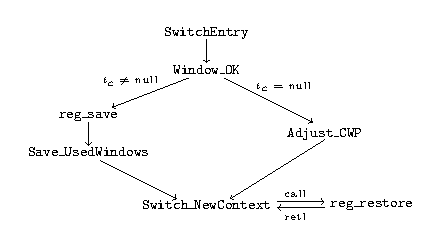
\includegraphics[scale=1.3]{picture//CodeStructure}
	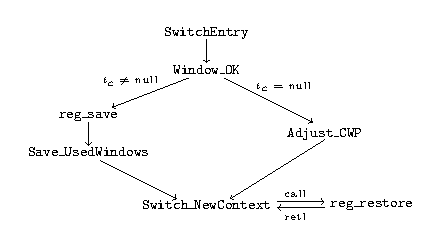
\includegraphics[scale=1.1]{picture//CodeStructure}
	\vspace{-0.4cm}
    \figurecaption{The Structure of Context Switch Module}
	\label{fig:The Structure of Context Switch Module}
\end{center}

% \begin{figure}[!t]
% 	\vspace{-0.8cm}
% 	\centering
% 	%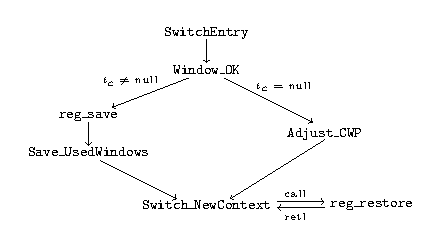
\includegraphics[scale=1.3]{picture//CodeStructure}
% 	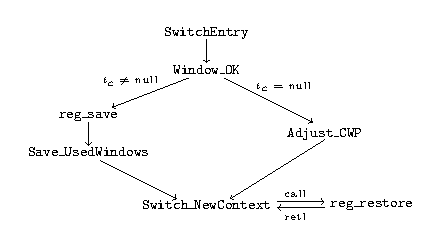
\includegraphics[scale=1.2]{picture//CodeStructure}
% 	\vspace{-0.4cm}
%     \caption{The Structure of Context Switch Module}
% 	\label{fig:The Structure of Context Switch Module}
% 	\vspace{-0.2cm}
% \end{figure}

\begin{itemize}
	\item
	\texttt{SwitchEntry}
    is the entry of the module.
	It checks {\tt SwitchFlag} to see if
    a context switch is needed. If yes,
    it enters the $\texttt{Window\_OK}$ block.
	
	\item
	\texttt{Window\_OK}
    checks if the current task is null (which may happen
    if the switch follows the delete of the current task).
    If yes, it jumps to \texttt{Adjust\_CWP}, which
    resets the pointer $\regcwp$ of the current register window
    so that it points to the last valid window. It essentially pops
    all the frames to empty the circular stack of register
    windows.
    If the current task is {\em not} null,
    it calls \texttt{reg\_save} to save the
    general registers into the TCB, and then
    enter the code block \texttt{Save\_UsedWindows}
    to save other register windows ($\Wstack$ in our
    state model).
	
	\item
	\texttt{Save\_UsedWindows} saves
	the register windows (except the current one)
    into the current task's stack in memory. 
    It checks whether the previous window is valid. 
    If it's valid, use the instruction $\crestore{}$ 
    to set the previous window as the current one, 
    and save its contents into stack (in memory), 
    then check the previous one continuously. 
	
	\item
	\texttt{Switch\_NewContext}
    %is responsible for
%	restoring the context stored in new task's TCB
%	and the other context saved in the top of the new task's stack.
%	Then it changes the new task as the current.
    restores the general registers and other register
    windows from the new task's TCB and its stack in memory,
    respectively. Then it sets the new task as
    the current one.
%    the new task's context from its TCB
%    and its stack in memory.
%    Then it changes the new task as the current one.
%>>>>>>> .r75
\end{itemize}

%\paragraph{\bf Challenge.}
The main complexity of the verification lies in
the code manages the register windows.
%The major difference between the context switch module we verified
%and a traditional one is caused by the register windows mechanism in \sparc{}.
%We have introduced that the register windows play as a role of circular stack.
%However, a stack in memory is still needed here because the number of windows is limited.
%
To save all the register windows, \texttt{Save\_UsedWindows}
repetitively restores the next window into general registers
(as the current window)
and then saves them into memory, until all the windows are saved.

%The code block \texttt{Save\_UsedWindows} is responsible
%for saving the contexts stored in register windows temporarily
%into current task's stack in memory when doing context switch.
%It restores the next window by window rotation and saves its contents into memory repeatedly,
%until the next window is an invalid one, which can be viewed a stack bottom.
%So, the implementation of \texttt{Save\_UsedWindows} is a loop
%and its verification work requires us to take more effort.

\paragraph{\textbf{Specification.}}
Below we give the pre- and post-conditions
($\apre$ and $\apost$) of the verified module.
Each of them takes 5 arguments,
the id of the current task $\ctid$, the id of the new
task $\ntid$, the value $\flag$ of the $\SwitchFlag$,
the values $\env$ of general registers and all
other register windows, and the new task's context $\nst$
that needs to be restored.
\[
    \small
    \begin{array}{l}
        \apre(\ctid, \ntid, \flag, \env, \nst) \ \define \\
        \qquad
        \begin{array}{l}
            \Env{\env} \sepstar (\msto{\SwitchFlag}{\flag}) \sepstar (\msto{\TaskNew}{\ntid})
            \sepstar \\
            \hspace*{8ex}
            (\flag\! =\! \afalse
            \vee \CurTask{\ctid}{\notCare}{\env}
                \!*\! \NoCurTask{\ntid}{\nst})
        \end{array}
        \\
        \\[-9pt]
        \apost(\ctid, \ntid, \flag, \env, \nst) \ \define \\
        \qquad
        \begin{array}{l}
            \Env{\env'} \sepstar (\msto{\SwitchFlag}{\afalse})
                    \sepstar (\msto{\TaskNew}{\ntid}) \sepstar
            \\
            \hspace*{8ex}
            (
            \flag \!=\! \afalse \land \pEnv{\env} \!=\! \pEnv{\env'}
            \\
            \quad \hspace*{8ex}
            \vee (\CurTask{\ntid}{\nst}{\env'} \land \pEnv{\env'}\!=\!\nst) *
            \\
            \quad \hspace*{12ex}
            \NoCurTask{\ctid}{\pEnv{\env}})        
        \end{array}
    \end{array}
    % \begin{array}{lcl}
    %     \apre(\ctid, \ntid, \flag, \env, \nst) & \define &
    %     \Env{\env} * (\msto{\SwitchFlag}{\flag}) * (\msto{\TaskNew}{\ntid}) * \\
    %     & & \hspace*{8ex}
    %     (\flag\! =\! \afalse
    %     \vee \CurTask{\ctid}{\notCare}{\env}
    %             \!*\! \NoCurTask{\ntid}{\nst}) \\
    %     %
    %     \apost(\ctid, \ntid, \flag, \env, \nst) & \define & \exists \env{}'. \
    %     \Env{\env'} * (\msto{\SwitchFlag}{\afalse})
    %                 * (\msto{\TaskNew}{\ntid}) *
    %     \\
    %     & & \hspace*{8ex}
    %     (
    %         \flag \!=\! \afalse \land \pEnv{\env} \!=\! \pEnv{\env'}
    %         \\
    %         & & \quad \hspace*{8ex}
    %         \vee (\CurTask{\ntid}{\nst}{\env'} \land \pEnv{\env'}\!=\!\nst) *
    %         \\
    %         & & \quad \hspace*{12ex}
    %         \NoCurTask{\ctid}{\pEnv{\env}})
    % \end{array}
\]

%specification of the key component of the context switch module verified,
%which is used to saving the current task's context and restore a new one.
%Five parameters are needed for specification that
%(1) $\ctid$ is the current task's identifier,
%(2) $\ntid$ is the new task's identifier,
%(3) $\flag$ presents the value of $\SwitchFlag$ which marks
%    whether there is a requirement to switch to a new task,
%(4) $\env$ presents the values stored in general registers and register windows,
%and
%(5) $\nst$ is the context of new task that will be restored.

In the specification,
we use $\Env{\env}$ to specify the values of
general registers and the register windows.
The variable $\TaskNew$ records the identifier of the new task.
If $\SwitchFlag$ is $\afalse$, we do not need any knowledge
about the current and the new tasks since there is no
context switch. Otherwise we describe the state
of the current task (its TCB and stack in memory)
using $\CurTask{\ctid}{\notCare}{\env}$,
and the saved context of the new task using
$\NoCurTask{\ntid}{\nst}$.
Due to space limitation we omit the detailed
definitions here.

If we compare $\apre$ and $\apost$, we can see that
$\ntid$ becomes the current task
($\CurTask{\ntid}{\nst}{\env'}$),
and its general registers and stack, specified by
$\Env{\env'}$, are loaded from the saved context
$\nst$ (\ie{} $\pEnv{\env'}\!=\!\nst$).
%$(\CurTask{\ntid}{\nst}{\env'} \land \pEnv{\env'}\!=\!\nst)$.
Here $\pEnv{\env'}$ refers to the part of the environment
that we want to save or restore as context.
Correspondingly, $\ctid$ becomes non-current-thread,
and part of its environment $\env$ at the entry of
the context switch is saved, as specified
by $\NoCurTask{\ctid}{\pEnv{\env}}$.

%\indent
%The precondition $\apre$ is shown below.
%The $\Env{\env}$ is used to describe the state of
%general registers and the register windows
%and uses $\env$ as parameter.
%The variable $\TaskNew$ records the identifier of the new task.
%We can see that if the value of the $\SwitchFlag$ is $\afalse$,
%we don't have to know anything about current task and new task,
%because there is no requirement to do context switch and
%the program exits directly.
%We describe the state of current task by $\CurTask{\ctid}{\notCare}{\env}$
%and the new task by $\NoCurTask{\ntid}{\nst}$.
%\[
%    \small
%    \begin{array}{lcl}
%        \apre(\ctid, \ntid, \flag, \env, \nst) & \define &
%        \Env{\env} * \msto{\SwitchFlag}{\flag} * \msto{\TaskNew}{\ntid} \\
%        & & \hspace*{12ex} * (\flag = \afalse \vee (\CurTask{\ctid}{\notCare}{\env} * \NoCurTask{\ntid}{\nst})) \\
%    \end{array}
%\]
%
%\indent
%We define the postcondition as $\apost$.
%It tells us that the new task $\ntid$ will become the
%current task and
%original current one will be the non-current task,
%if the $\flag$ is $\atrue$.
%Here, the $\pEnv{\env}$ is used to extract part
%of dates that the task hopes to save.
%%\[
%%    \small
%%    \begin{array}{lcl}
%%        \apost(\ctid, \ntid, \flag) & \define &
%%        \exists \env, \cst, \nst. \\
%%        & & \ \
%%        \Env{\env} * \msto{\SwitchFlag}{\afalse} * \msto{\TaskNew}{\ntid} \\
%%        & & \ \
%%        * (\flag = \afalse \, \vee \,
%%            (\flag = \atrue \, \land \, (\CurTask{\ntid}{\nst}{\env} * \NoCurTask{\ctid}{\cst}))
%%        )
%%    \end{array}
%%\]
%\[
%    \small
%    \begin{array}{lcl}
%        \apost(\ctid, \ntid, \flag, \env, \nst) & \define & \exists \env{}'. \
%        \Env{\env'} * \msto{\SwitchFlag}{\afalse} * \msto{\TaskNew}{\ntid} \\
%        & & *
%        (
%            (\flag = \afalse \land \pEnv{\env} = \pEnv{\env'}) \\
%            & & \quad \vee (\CurTask{\ntid}{\nst}{\env'} * \NoCurTask{\ctid}{\pEnv{\env}}))
%    \end{array}
%\]
%

%\indent
%The $\NoCurTask{\tid}{\tskst}$ describes the state of task $\tid$'s
%context structure and stack in memory, if $\tid$ is not \Null{}. The context structure,
%which is a part of TCB  for registers data saving, is presented as
%$\context{\tid + \offsetctx, \ctx}$, where its address is $\tid + \offsetctx$.
%And $\stackCons{\stk}$ presents the state of task's stack in memory.
%Here $\Top$ is the address of stack top and $\stkcont$ is the values
%saved in stack.
%The $\stkfmPt{\Top}{\env}$ used in $\CurTask{\tid}{\tskst}{\env}$
%illustrates a pointing relationship between register windows and task's stack.
%It says that each context saved in register windows temporarily records a pointer that points to
%a stack frame in stack where it will be stored.
%\[
%    \small
%    \begin{array}{lcl}
%        \NoCurTask{\tid}{\tskst} & \define &
%        (\tid \neq \Null \, \land \, (\context{\tid + \offsetctx, \ctx} * \stackCons{\stk}))
%        \, \vee \, \tid = \Null
%        \\
%        & & \ \ {\text{where} \ \tskst = (\ctx, \stk), \, \stk = (\Top, \stkcont)} \\
%        \\[-8pt]
%        \CurTask{\tid}{\tskst}{\env} & \define &
%        (\msto{\TaskCur}{\tid} * \NoCurTask{\tid}{\tskst}) \, \land \,
%        \stkfmPt{\Top}{\env} \\
%        & & \ \ {\text{where} \ \tskst = (\ctx, \stk), \, \stk = (\Top, \stkcont)}
%    \end{array}
%\]
\begin{figure*}[!t]
    \[
        \begin{array}{c}
            \infer[L_3]
            {
                (\regst{\regN}{\val}) \sepstar \astP_1 \Longrightarrow 
                (\regst{\regN}{\val}) \sepstar \astP_2
            }
            {
                \astP_1 \Longrightarrow \astP_2
            } \qquad 
            \infer[L_4]
            {
                (\dlyregst{t}{\st}{\word}) \sepstar \astP_1 \Longrightarrow 
                (\dlyregst{t}{\st}{\word}) \sepstar \astP_2
            }
            {
                \astP_1 \Longrightarrow \astP_2
            } \\
            \\[-5pt]
            \infer[L_3]
            {
                \nxtAst{(\dlyregst{0}{\sr}{\word})} \sepstar \astP_2 \Longrightarrow 
                (\regst{\sr}{\word}) \sepstar \astP_2
            }
            {
                \astP_1 \Longrightarrow \astP_2
            } \quad \ \ 
            \infer[L_4]
            {
                \nxtAst{(\dlyregst{t+1}{\sr}{\word})} \sepstar \astP_1 \Longrightarrow 
                (\dlyregst{t}{\sr}{\word}) \sepstar \astP_2
            }
            {
                \astP_1 \Longrightarrow \astP_2
            } \\
            \\[-5pt]
            \infer[L_5]
            {
                \nxtAst{(\regst{\regN}{\val})} \sepstar \astP_1 \Longrightarrow 
                \regst{\regN}{\val} \sepstar \astP_2
            }
            {
                \astP_1 \Longrightarrow \astP_2
            } \qquad 
            \infer[L_6]
            {
                \nxtAst{(\sepsto{\loc}{\val})} \sepstar \astP \Longrightarrow 
                (\sepsto{\loc}{\val}) \sepstar \astP'
            }
            {
                \astP_1 \Longrightarrow \astP_2
            } \quad \ \
            \infer[L_7]
            {
                \nxtAst{(\astP_1 \sepstar \astP_2)}
                \Longrightarrow 
                \astP_1' \sepstar \astP_2'
            }
            {
                \nxtAst{\astP_1} \Longrightarrow \astP_1' \quad \ \ 
                \nxtAst{\astP_2} \Longrightarrow \astP_2'
            } 
        \end{array}
    \]
    \caption{Extended rules for Tactic \sepcancel{}}
    \label{fig:ext-rule-tac-sepcancel}
\end{figure*}
\paragraph{\textbf{Tactics for Automated Reasoning.}} 
\etal{Cao}\cite{practical-tactics} propose a set of practical tactics 
for verifiying C program in Coq. 
including \sepcancel{}, which uses some 
inference rules (\eg{} $L_1$ and $L_2$ shown as following) 
repeatedly to solve $\astP \Longrightarrow \astQ$. 
\[
    \small
    \infer[L_1]
    {
        \astP_1 \sepstar \astQ' \Longrightarrow \astP_2 \sepstar \astQ'
    }
    {
        \astP_1 \Longrightarrow \astP_2
    } \quad \ \  
    \infer[L_2]
    {
        (\sepsto{\loc}{\val}) \sepstar \astP_1 \Longrightarrow 
        (\sepsto{\loc}{\val}) \sepstar \astP_2
    }
    {
        \astP_1 \Longrightarrow \astP_2
    }
\]
One of a important tacitc in their work is \sepcancel{}. 
It has a library, including some rules (\eg{} $L_1$ and $L_2$ shown above), 
and uses the rules in library repeatedly to solve 
``$\astP \Longrightarrow \astQ$". The rules $L_1$ and $L_2$  
let we can use \sepcancel{} to eliminate the 
subterms, which describe the same resources, 
in $\astP$ and $\astQ$.
Recalling the introduction in \Sec{\ref{subsec:assertions}}, 
registers in our work are also treated as resource. 
So, we extend the inference rules used by original \sepcancel{} tactics
and let it  

Recalling the introduction in \Sec{\ref{subsec:assertions}}, 
registers in our work are also treated as resource, like memory location. 
In our work, we add some additional rules $L_3 \sim L_7$ 
(defined in \Fig{\ref{fig:ext-rule-tac-sepcancel}})
to the library of \sepcancel{}. The soundness of rules $L_3 \sim L_7$ 
can be achieved from the properties of assertions introduced in 
\Sec{\ref{subsec:assertions}} directly. Aftering extending the original 
\sepcancel{} tactic, we can find that the correctness proof
of the following implication can be accomplished by using 
the extended \sepcancel{} directly.
\begin{multline*}
    \nxtAst{(\dlyregst{3}{\regY}{\word_1} \sepstar 
    \dlyregst{0}{\regwim}{\word_2} \sepstar 
    \regst{\reg{5}}{\val})} \Longrightarrow \\
    \dlyregst{2}{\regY}{\word_1} \sepstar 
    \regst{\regwim}{\word_2} \sepstar 
    \regst{\reg{5}}{\val}
\end{multline*}
\[
    \nxtAst{(\dlyregst{3}{\regY}{\word_1} \sepstar 
    \dlyregst{0}{\regwim}{\word_2} \sepstar 
    \regst{\reg{5}}{\word_3})} \Longrightarrow 
    \dlyregst{2}{\regY}{\word_1} \sepstar 
    \regst{\regwim}{\word_2} \sepstar 
    \regst{\reg{5}}{\word_3}
\] 
Using the extended \sepcancel{} can greatly simplify our verification 
work, and improve the efficiency of code proving. 

\paragraph{\textbf{Proof Efforts in Coq.}}
We omit the code that manages interrupt
and float registers in the original
system, which are not supported in our logic.
%because our current work doesn't consider them.
The segment we verify has around 250 lines
of assembly code,
and we verify it by 6690 lines of %(including the tactics and libraries)
Coq proof scripts.

% We briefly show how we verify the 
% context switch routine in Coq using our program logic. 
% % % \begin{figure}[!t]
%     \centering
%     \small
%     \[
%         \begin{array}{c|c}
%         \begin{array}{l}
%             {\tt Theorem \ \ CtxSwitch\_Correct: } \\
%             \qquad 
%             {\tt wf\_cdhp \ \, spec \ C}. \\
%             {\tt Proof. }  \\
%             \qquad \dots \ \ \dots \ \ \dots \\ 
%             {\tt Qed. }
%         \end{array} \quad & \quad
%         \begin{array}{l}
%             {\tt Lemma \ \ SwitchEntryProof: } \\
%             \qquad 
%             {\tt forall \ vl,} \\
%             \qquad \qquad
%             {\tt spec \ |- \ \{\{ \ \colorbox{yellow!80}{switch\_entry\_pre \ vl} \ \}\} } \\
%             \qquad \qquad \qquad \qquad \qquad
%             {\tt f0 : switch\_entry\_code} \\
%             \qquad \qquad \qquad \qquad
%             {\tt \ \{\{ \ \colorbox{yellow!80}{switch\_entry\_post \ vl} \ \}\}. } \\
%             {\tt Proof.} \\
%             \qquad \dots \ \ \dots \ \ \dots \\ 
%             {\tt Qed. }
%         \end{array} \\
%         \\[-5pt]
%         \text{(a)} & \text{(b)}
%         \end{array}
%     \]
%     \caption{Example of Context Switch Routine Proof in Coq}
%     \label{fig:CorrectCtx-Coq}
%     \vspace{-0.5em}
% \end{figure}

\begin{figure}[!t]
    \centering
    \small
    \[
        \begin{array}{c|c}
        \begin{array}{l}
            {\tt Theorem \ \ CtxSwitch\_Correct: } \\
            \qquad 
            {\tt wf\_cdhp \ \, spec \ C}. \\
            {\tt Proof. }  \\
            \qquad \dots \ \ \dots \ \ \dots \\ 
            {\tt Qed. }
        \end{array} \quad & \quad
        \begin{array}{l}
            {\tt Lemma \ \ SwitchEntryProof: } \\
            \qquad 
            {\tt forall \ vl,} \\
            \qquad \qquad
            {\tt spec \ |- \ \{\{ \ \colorbox{yellow!80}{switch\_entry\_pre \ vl} \ \}\} } \\
            \qquad \qquad \qquad \qquad \qquad
            {\tt f0 : switch\_entry\_code} \\
            \qquad \qquad \qquad \qquad
            {\tt \ \{\{ \ \colorbox{yellow!80}{switch\_entry\_post \ vl} \ \}\}. } \\
            {\tt Proof.} \\
            \qquad \dots \ \ \dots \ \ \dots \\ 
            {\tt Qed. }
        \end{array} \\
        \\[-5pt]
        \text{(a)} & \text{(b)}
        \end{array}
    \]
    \caption{Example of Context Switch Routine Proof in Coq}
    \label{fig:CorrectCtx-Coq}
    \vspace{-0.5em}
\end{figure}
% \begin{center}
%     \vspace*{-0.8cm}
%     $$ \ 
%     {\tt Theorem \ \ CtxSwitch\_Correct: } \ \ 
%     {\tt wf\_cdhp \ \, spec \ C}.
%     $$
%     $$
%     \begin{array}{l}
%         {\tt Lemma \ \ SwitchEntryProof: } \\
%         \qquad 
%         {\tt forall \ vl,} \\
%         \qquad \qquad
%         {\tt spec \ |- \ \{\{ \ \colorbox{yellow!80}{switch\_entry\_pre \ vl} \ \}\} } \\
%         \qquad \qquad \qquad \qquad \qquad
%         {\tt f0 : switch\_entry\_code} \\
%         \qquad \qquad \qquad \qquad
%         {\tt \ \{\{ \ \colorbox{yellow!80}{switch\_entry\_post \ vl} \ \}\}. }
%     \end{array}
%     $$
%     \figurecaption{Coq Code Example}
%     \label{fig:Coq code Example}
% \end{center}
% % \begin{figure}[!t]
% %     \centering
% %     \small
% %     \[
% %         \begin{array}{c|c}
% %         \begin{array}{l}
% %             {\tt Theorem \ \ CtxSwitch\_Correct: } \\
% %             \qquad 
% %             {\tt wf\_cdhp \ \, spec \ C}. \\
% %             {\tt Proof. }  \\
% %             \qquad \dots \ \ \dots \ \ \dots \\ 
% %             {\tt Qed. }
% %         \end{array} \quad & \quad
% %         \begin{array}{l}
% %             {\tt Lemma \ \ SwitchEntryProof: } \\
% %             \qquad 
% %             {\tt forall \ vl,} \\
% %             \qquad \qquad
% %             {\tt spec \ |- \ \{\{ \ \colorbox{yellow!80}{switch\_entry\_pre \ vl} \ \}\} } \\
% %             \qquad \qquad \qquad \qquad \qquad
% %             {\tt f0 : switch\_entry\_code} \\
% %             \qquad \qquad \qquad \qquad
% %             {\tt \ \{\{ \ \colorbox{yellow!80}{switch\_entry\_post \ vl} \ \}\}. } \\
% %             {\tt Proof.} \\
% %             \qquad \dots \ \ \dots \ \ \dots \\ 
% %             {\tt Qed. }
% %         \end{array} \\
% %         \\[-5pt]
% %         \text{(a)} & \text{(b)}
% %         \end{array}
% %     \]
% %     \caption{Example of Context Switch Routine Proof in Coq}
% %     \label{fig:CorrectCtx-Coq}
% %     \vspace{-0.5em}
% % \end{figure}
% The Coq theorem named ``{\tt CtxSwitch\_Correct}" in 
% \Fig{\ref{fig:Coq code Example}} is the final theorem of 
% the correctness of context routine in Coq.
% % \Fig{\ref{fig:CorrectCtx-Coq}} (a) is the final theorem of 
% % the correctness of context routine in Coq. The 
% % ``{\tt CtxSwitch\_Correct}" is the name of this 
% % theorem. And 
% The ``{\tt wf\_cdhp spec C}" is the  
% Coq implementation of well-formed code heap 
% ``$\wfcdhp{\code}{\Cspec}$". Here, the code heap 
% ``{\tt C}" is the code heap storing the context 
% switch code, and ``{\tt spec}" is the specifications 
% of each code block shown in 
% \Fig{\ref{fig:The Structure of Context Switch Module}}. 
% The correctness of this theorem can be proved by the 
% definition of well-formed code heap, which is defined 
% as ``{\tt wf\_cdhp}" in Coq. According to the 
% definition of ``$\wfcdhp{\code}{\Cspec}$" in 
% \Fig{\ref{fig:Seleted Inference rules}}, we need to 
% prove the correctness of each code block in code heap shown in 
% \Fig{\ref{fig:The Structure of Context Switch Module}}. 
% We use \texttt{SwitchEntry} as an example 
% of proving the correctness of code block 
% (instruction sequence) in Coq. 
% The Coq lemma ``\texttt{SwitchEntryProof}" in 
% \Fig{\ref{fig:Coq code Example}}
% describes the correctness of \texttt{SwitchEntry} 
% in Coq. This lemma can be viewed as the a Coq implementation 
% of the following properties. 
% \[
%     \text{for all } \, \lgvl. \ 
%     \wfcblk{\apre \ \lgvl}{\apost \ \lgvl}{\lab{0}}
%         {\texttt{SwitchEntry}}
% \]
% As shown in \Fig{\ref{fig:The Structure of Context Switch Module}}, 
% the {\texttt{SwitchEntry}} is the entry of the context switch 
% routine. So, it's specification is the $\apre$ and $\apost$ defined 
% before, according to the meaning of the specification of a code block. 
% % The name of this lemma is \texttt{SwitchEntryProof} in Coq. 
% The ``{\tt switch\_entry\_pre}" and ``{\tt switch\_entry\_post}" 
% are Coq implementations of $\apre$ and $\apost$. 
% The ``{\tt vl}" and ``{\tt f0}" are logical variables 
% and the starting label of code block {\texttt{SwitchEntry}} in Coq 
% respectively. And the code block {\tt SwitchEntry} is defined as 
% ``{\tt switch\_entry\_code}" in Coq, which is an instruction sequence 
% extracted from label ``{\tt f0}" in code heap ``{\tt C}". 

Readers may find that the \textbf{CALL} rule in our logic,
defined in \Fig{\ref{fig:Seleted Inference rules}}, doesn't 
support the calling of the context switch routine, because 
the switching of return pointer isn't permitted. We don't 
consider to solve this problem by modifying our \textbf{CALL} 
rule, but address it in another way in the next section, 
proving the context refinement between context switch routine 
and its abstract assembly primitive $\primsw$. The \textbf{CALL} 
rule is just used for verifying the internal functions. 

% We address 
% this problem in the next section about refinement verification. 
% After the introducation of the next section, we can find that 
% there is no problem to prove the context refinement between 
% context switch routine and its abstract assembly primitive 
% $\primsw$, because they will set the program counters 
% in low- and high-level to the same code pointer after 
% execution. 
  \section{Refinement Verification of SPARCv8}
\label{sec:refine-verification-sparc}

Inspired by the {\it relational} program logic for 
refinement verification, \eg{\cite{liang13pldi,Xu16cav}}, 
we extend our program logic for SPARCv8 to support
refinement verification in this section. 
We first define the high- and low-level program in 
\Sec{\ref{subsec:High-level Pseudo-SPARCv8 Language}} and 
\Sec{\ref{subsec:low-level SPARCv8 Program}} respectively, 
and their state relation in \Sec{\ref{subsec:state-rel}}. 
The refinement relation is represented in 
\Sec{\ref{subsec:correctness-primitive}}, 
and program logic is shown in 
\Sec{\ref{subsec:rel-assertion}} and 
\Sec{\ref{subsec:logic-rule-refinemet}}, 
including the relational assertion language 
and inference rules.  
Finally, logic soundness is shown in 
\Sec{\ref{subsec:logic-ensuring-ctxrefinement}}.

\subsection{High-level Pseudo-SPARCv8 Language}
\label{subsec:High-level Pseudo-SPARCv8 Language}
% The target program in our work is SPARCv8, which is 
% introduced in \Sec{\ref{sec:modeling}}. So,  
% We choose the SPARCv8 program defined in 
% \Sec{\ref{sec:modeling}} as the {\it low-level} 
% program. And 

We define the Pseudo-SPARCv8 language in this 
subsection. It contains two part: 
the SPARCv8 code as client code, 
and the set of abstract assembly primitives. 
Here, we require that the execution of client SPARCv8 code 
preserves a restriction between register 
window and stack in memory, shown
as the left side in \Fig{\ref{fig:Abstraction of Register Windows and Memory}}
(\regcwp{} points to the current window and \regwim{} marks 
the invalid window, the details of overlapping 
of adjacent windows are omitted in the figure).
\begin{center}
    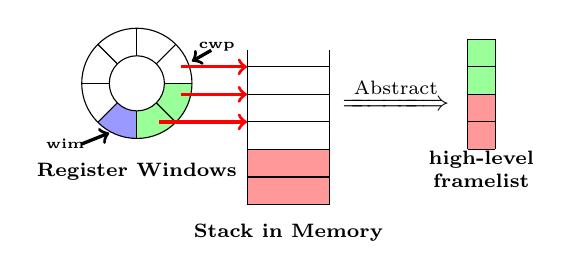
\begin{tikzpicture}[scale=0.7]
    \fill[green!40!white] (0,0) -- (0,-1cm) arc (-90:0:1cm) -- (0,0);
    \fill[blue!40!white] (0,0) -- (0,-1cm) arc (-90:-135:1cm) -- (0,0);
    % \fill[yellow!80!white] (0,0) -- (0,-1cm) arc (-90:-135:1cm) -- (0,0);
    % \fill[blue!40!white] (0,0) -- (-1,0cm) arc (-180:-135:1cm) -- (0,0);
    \draw (0, 0) -- (90:1cm);
    \draw (0, 0) -- (45:1cm);
    \draw (0, 0) -- (0:1cm);
    \draw (0, 0) -- (-45:1cm);
    \draw (0, 0) -- (-90:1cm);
    \draw (0, 0) -- (-135:1cm);
    \draw (0, 0) -- (-180:1cm);
    \draw (0, 0) -- (135:1cm);
    \fill[white] (0, 0) circle (0.5cm);
    \draw (0, 0) circle (1cm);
    \draw (0, 0) circle (0.5cm);
    % \draw[very thick, blue] (0, -0.3) -- (0, -1.2);
    % \draw[very thick, blue] (0, -0.32) -- (0.1, -0.32);
    % \draw[very thick, blue] (0, -1.18) -- (0.1, -1.18);
    \node(wim) at (-1.3, -1.1) {\tiny \bf wim};
    \draw[->, very thick] (-1, -1.1) -- (-0.5, -0.9);

    % \node(wim) at (-1.7, -0.7) {\tiny \bf wim};
    % \draw[->, very thick] (-1.5, -0.6) -- (-1, -0.4);
    

    \node(cwp) at (1.45, 0.67) {\tiny \bf cwp};
    \draw[->, very thick] (1.35, 0.6) -- (1, 0.4);

    \node(regwin) at (0, -1.6) {\scriptsize \bf Register Windows};

    %%%%%%%%%%%%%%%%%%%%%%%%%%%%%%%%%%%%%%%%%%%%%%%%%%%%%%

    \fill[red!40!white] (2, -1.2) rectangle (3.5, -1.7);
    \fill[red!40!white] (2, -1.7) rectangle (3.5, -2.2);

    \draw[-] (2, 0.6) -- (2, -2.2);
    \draw[-] (3.5, 0.6) -- (3.5, -2.2);
    
    \draw[-] (2, 0.3) -- (3.5, 0.3);
    \draw[-] (2, -0.2) -- (3.5, -0.2);
    \draw[-] (2, -0.7) -- (3.5, -0.7);
    \draw[-] (2, -1.2) -- (3.5, -1.2);
    \draw[-] (2, -1.7) -- (3.5, -1.7);
    \draw[-] (2, -2.2) -- (3.5, -2.2);

    \node(stkfm) at (2.75, -2.7) {\scriptsize \bf Stack in Memory};

    %%%%%%%%%%%%%%%%%%%%%%%%%%%%%%%%%%%%%%%%%%%%%%%%%%%%%%%

    \draw[->, very thick, red] (0.8, 0.3) -- (2, 0.3);
    \draw[->, very thick, red] (0.8, -0.2) -- (2, -0.2);
    \draw[->, very thick, red] (0.4, -0.7) -- (2, -0.7);

    %%%%%%%%%%%%%%%%%%%%%%%%%%%%%%%%%%%%%%%%%%%%%%%%%%%%%%

    \node(abstract) at (4.7, -0.2) {$\xLongrightarrow{\text{Abstract}}$};

    %%%%%%%%%%%%%%%%%%%%%%%%%%%%%%%%%%%%%%%%%%%%%%%%%%%%%%

    \fill[green!40!white] (6, 0.8) rectangle (6.5, 0.3);
    \fill[green!40!white] (6, 0.3) rectangle (6.5, -0.2);
    \fill[red!40!white] (6, -0.2) rectangle (6.5, -0.7);
    \fill[red!40!white] (6, -0.7) rectangle (6.5, -1.2);

    \draw[-] (6, 0.8) -- (6, -1.2);
    \draw[-] (6.5, 0.8) -- (6.5, -1.2);

    \draw[-] (6, 0.8) -- (6.5, 0.8);
    \draw[-] (6, 0.3) -- (6.5, 0.3);
    \draw[-] (6, -0.2) -- (6.5, -0.2);
    \draw[-] (6, -0.7) -- (6.5, -0.7);
    \draw[-] (6, -1.2) -- (6.5, -1.2);

    \node(hfrmlist) at (6.25, -1.6) 
        {
            \scriptsize \bf
            $
            \begin{array}{c}
                \text{high-level} \\
                \text{framelist}
            \end{array}
            $
        };
\end{tikzpicture} 
    \vspace*{-0.5em}
    \figurecaption{Abstraction of context management}
    \label{fig:Abstraction of Register Windows and Memory}
    \vspace{-0.5em}
\end{center}
During the SPARCv8 program's execution, 
part of previous procedures' contexts 
(the green part in the left side of the 
\Fig{\ref{fig:Abstraction of Register Windows and Memory}}) 
are saving in register window, the others 
(the pink part in the left side of the 
\Fig{\ref{fig:Abstraction of Register Windows and Memory}})
are stored in stack in memory, 
% (shown as the red arrow in 
% \Fig{\ref{fig:Abstraction of Register Windows and Memory}}), 
because the number of windows is limited. 
The restriction is that the stack pointer 
(\spreg{}) of each procedure, 
including the current one and the previous one, 
whose contexts are saved in register 
window currently, should point to the top of its stack frame 
(shown as the red arrow in 
\Fig{\ref{fig:Abstraction of Register Windows and Memory}}),
so that the contexts 
in these windows can be stored correctly 
in memory when needed. For instance, as  
introduced in \Sec{\ref{sec:ctxswitch}}, the 
context switch routine will check 
whether the previous window is valid 
(in clockwise direction in 
\Fig{\ref{fig:Abstraction of Register Windows and Memory}}), 
and use instruction $\crestore{}$ to set it as the 
current one and save its contents into stack 
(in memory) until the previous one is invalid 
(marked in blue in \Fig{\ref{fig:Abstraction of Register Windows and Memory}}). 
We require the execution of client code 
preserving such restriction. Otherwise, some SPARCv8 
functions like context switch routine whose 
implementations will store the contexts saved in 
register window into stack in memory cannot be 
verified if it's unclear where to save the 
contents of some windows. 
% We require the execution of client code 
% preserving this relation so that the relation 
% holds when calling context switch routine. 
% \footnote{The requirement for client code
% preserving such relation will not restrict the 
% application of our work, because such relation
% is also mentioned as a SPARCv8 programming 
% convention in The SPARC Architecture Manual(version 8)~\cite{sparc},
% which says that "It is essential 
% that \spreg{} always contains the correct value, 
% so that when (and if) a register window overflow/underflow trap occurs, 
% the register window can be correctly stored to or reloaded from memory "}.
% Otherwise, the correctness of context switch 
% routine can't be proved if we are unclear where 
% to save the contents of some windows. 
We do the following when defining 
Pseudo-SPARCv8 program to make the execution 
of client code preserves such restriction:  
\begin{itemize}
    \item
    In order to ensure that 
    the stack pointer (\spreg{}) always 
    point to the top of its stack frame, we require that   
    each instruction, like \cadd{} and \ld{}, whose 
    execution will not rotate register window, 
    is not allowed to update the value of \spreg{}; 
    and as for the \csave{} and \crestore{}, whose executions 
    will rotate register window, we restrict them 
    to be used in specific forms. 
    We introduce ``$\Psave \ \word$" as a macro of 
    ``$\csave{} \ \spreg, -\word, \spreg$", 
    whose execution makes sure that a new \spreg{} 
    will be generated for the next window
    and point to the stack frame size $w$ allocated newly. 
    We also introduce ``$\Prestore$" 
    as a macro of ``$\crestore{} \ \greg{0}, \greg{0}, \greg{0}$"
    \footnote{In SPARCv8, $\greg{0}$ is always equal to 0, 
    and usually used as parameters when instructions do not 
    require specific parameters.},  
    whose execution just restores the previous window 
    and doesn't modify the value of any register 
    in the previous window restored. 
    The original \csave{} and \crestore{} instructions 
    have \textit{no} semantics in high-level client code.   
    
    % The \csave{} and \crestore{} instructions that operate  
    % register window can't be used arbitrarily. 
    % When we use \csave{} to rotate to next window
    % (counterclockwise direction in \Fig{\ref{fig:Abstraction of Register Windows and Memory}}),  
    % a new stack pointer \spreg{} should 
    % be generated to point to the stack frame 
    % in memory allocated newly. 
    % And when we use \crestore{} to rotate to previous window 
    % (in clockwise direction in \Fig{\ref{fig:Abstraction of Register Windows and Memory}}), 
    % its execution shouldn't modify x
    % the value of \spreg{} in the previous window.
    % % So as to preserve the requirement that each 
    % % stack pointer (\spreg) points 
    % % to its corresponding stack frame
    % % during the execution of client code,  
    % % the execution of \csave{} should generate a new 
    % % \spreg{} pointing to the stack frame in 
    % % memory allocated newly, and the execution of 
    % % \crestore{} shouldn't modify the value of 
    % % \spreg{} in the window restored.  
    % So, we introduce ``$\Psave \ \word$" as a macro of 
    % ``$\csave{} \ \spreg, -\word, \spreg$", 
    % whose execution makes sure that a new \spreg{} 
    % will be generated and point to the stack frame 
    % size $w$ allocated newly. 
    % We also introduce ``$\Prestore$" 
    % as a macro of ``$\crestore{} \ \greg{0}, \greg{0}, \greg{0}$"
    % \footnote{In SPARCv8, $\greg{0}$ is always equal to 0, 
    % and usually used as parameters when instructions do not 
    % require specific parameters.},  
    % whose execution just restores the previous window 
    % and doesn't modify any register value. 
    % The original \csave{} and \crestore{} instructions 
    % have \textit{no} semantics in high-level client code. 

    \item 
    The special registers can't be modified arbitrarily.
    The special registers in SPARCv8 usually act specific 
    roles and modifying them should be carefully, 
    for example, \regwim{} marks which window is 
    invalid. If we change its value shown in 
    \Fig{\ref{fig:Abstraction of Register Windows and Memory}}, 
    to mark another window invalid, as shown in 
    \Fig{\ref{fig:problem of modifying wim arbitrary}},  
    \begin{center}
        \vspace*{-0.5em}
        \begin{tikzpicture}[scale=0.75]
    \pgfdeclarepatternformonly{my crosshatch dots}{\pgfqpoint{-1pt}{-1pt}}{\pgfqpoint{2.5pt}{2.5pt}}{\pgfqpoint{3pt}{3pt}}
    {
        \pgfpathcircle{\pgfqpoint{0pt}{0pt}}{.4pt}
        \pgfpathcircle{\pgfqpoint{1.5pt}{1.5pt}}{.4pt}
        \pgfusepath{fill}
    }

    \fill[gray!20] (0,0) -- (0,-1cm) arc (-90:0:1cm) -- (0,0);
    \fill[pattern=my crosshatch dots] (0,0) -- (0,-1cm) arc (-90:-135:1cm) -- (0,0);
    \fill[pattern=north east lines] (0,0) -- (-1,0cm) arc (-180:-135:1cm) -- (0,0);
    \draw (0, 0) -- (90:1cm);
    \draw (0, 0) -- (45:1cm);
    \draw (0, 0) -- (0:1cm);
    \draw (0, 0) -- (-45:1cm);
    \draw (0, 0) -- (-90:1cm);
    \draw (0, 0) -- (-135:1cm);
    \draw (0, 0) -- (-180:1cm);
    \draw (0, 0) -- (135:1cm);
    \fill[white] (0, 0) circle (0.5cm);
    \draw (0, 0) circle (1cm);
    \draw (0, 0) circle (0.5cm);

    \node(wim) at (-1.7, -0.7) {\tiny \bf wim};
    \draw[->, line width=0.5pt] (-1.5, -0.6) -- (-1, -0.4);
    

    \node(cwp) at (1.45, 0.67) {\tiny \bf cwp};
    \draw[->, line width=0.5pt] (1.35, 0.6) -- (1, 0.4);

    \node(regwin) at (0, -1.6) {\scriptsize Register Windows};

    %%%%%%%%%%%%%%%%%%%%%%%%%%%%%%%%%%%%%%%%%%%%%%%%%%%%%%

    \fill[black!50] (2, -1.2) rectangle (3.3, -1.7);
    \fill[black!50] (2, -1.7) rectangle (3.3, -2.2);

    \draw[-] (2, 0.6) -- (2, -2.2);
    \draw[-] (3.3, 0.6) -- (3.3, -2.2);
    
    \draw[-] (2, 0.3) -- (3.3, 0.3);
    \draw[-] (2, -0.2) -- (3.3, -0.2);
    \draw[-] (2, -0.7) -- (3.3, -0.7);
    \draw[-] (2, -1.2) -- (3.3, -1.2);
    \draw[-] (2, -1.7) -- (3.3, -1.7);
    \draw[-] (2, -2.2) -- (3.3, -2.2);

    \node(stkfm) at (2.75, -2.7) {\scriptsize Stack in Memory};

    %%%%%%%%%%%%%%%%%%%%%%%%%%%%%%%%%%%%%%%%%%%%%%%%%%%%%%%

    \draw[->, line width=0.8pt] (0.8, 0.3) -- (2, 0.3);
    \draw[->, line width=0.8pt] (0.8, -0.2) -- (2, -0.2);
    \draw[->, line width=0.8pt] (0.4, -0.7) -- (2, -0.7);

    %%%%%%%%%%%%%%%%%%%%%%%%%%%%%%%%%%%%%%%%%%%%%%%%%%%%%%

    % \node(abstract) at (4.7, -0.2) {$\xLongrightarrow{\text{Abstract}}$};

    %%%%%%%%%%%%%%%%%%%%%%%%%%%%%%%%%%%%%%%%%%%%%%%%%%%%%%
\end{tikzpicture} 
        \figurecaption{Problem of modifying 
        \regwim{} arbitrary}
        \vspace*{-0.5em}
        \label{fig:problem of modifying wim arbitrary}
    \end{center}
    and call context switch routine, which will  
    save the contents of previous windows into memory
    until the invalid one, at this moment. 
    There will be a problem that we don't know 
    where to save the contents of window that 
    is marked invalid originally 
    (window in yellow in \Fig{\ref{fig:problem of modifying wim arbitrary}}). 
    % Supposing the register window and  
    So, we don't allow client code 
    to modify special registers and do \textit{not} 
    give semantics to \cwr{} instruction in high-level 
    client code. Modifying them is hidden in the 
    implementation of the abstract assembly primitives
    in low-level. 
    The delay buffer can be omitted in high-level
    program state. 
    % omit them 
    % in the Pseudo-SPARCv8 program state. Operating them 
    % is hidden in the implementation of the 
    % abstract assembly primitives. 
    % We also do \textit{not} give semantics to 
    % \cwr{} and \rd{} instructions in high-level 
    % client code. 
    \item 
    As shown in \Fig{\ref{fig:Abstraction of Register Windows and Memory}}, 
    we find that we can abstract the register window 
    and the memory in stack for storing contexts 
    as a list (defined as 
    HFrmList formally in \Fig{\ref{fig:machine-state-concur-pseudo-sparc}}).  
    After this abstraction, We don't need to care about 
    whether the contexts are saved in register window or 
    memory and describe the contents of windows unused 
    (the windows in white color in 
    \Fig{\ref{fig:Abstraction of Register Windows and Memory}}, 
    but excluding the current one pointed by \regcwp{}) 
    in the Pseudo-SPARCv8 level. 
    The \regcwp{} register is no longer needed in 
    Pseudo-SPARCv8 program because the register window 
    is abstracted away. 
    The low-level program in our work doesn't use this 
    abstraction, because the low-level program 
    should be realistically modelled, 
    and the implementations of some primitives 
    need to know the existance of register window,  
    for instance, the context switch routine 
    needs to save the contents 
    of the register window into stack (in memory).
\end{itemize}

\begin{figure*}[!t]
    \centering
    \vspace{-2em}
    \small
    \[
        \begin{array}{rcclcrccl}
            \TYPE{(HCode)} & \ \HMd \ & \define & (\code, \hprimset) & & 
            \qquad\,
            \TYPE{(CodeHeap)} & \ \code \ & \in & \TYPE{Word} \rightharpoonup \TYPE{Comm} 
            \\
            \\[-8pt]
            \TYPE{(PrimSet)} & \hprimset & \define & 
            \multicolumn{6}{l}
                {
                    \{ \lab{1} \rightsquigarrow \hprim_1, \dots, \lab{n} \rightsquigarrow \hprim_n \}
                    \qquad\quad
                    \TYPE{(Prim)} \ \ \hprim \ \in \ 
                    \TYPE{List} \ \TYPE{Val} \rightarrow \TYPE{HState} \rightarrow 
                    \TYPE{HState} \rightarrow \TYPE{Prop}            
                }  \\
            \\
            % \TYPE{(Prim)} & \hprim & \in & 
            % \multicolumn{6}{l}
            % {
            %     \TYPE{List} \ \TYPE{Val} \rightarrow \TYPE{HState} \rightarrow 
            %     \TYPE{HState} \rightarrow \TYPE{Prop}
            % } \\
            % \TYPE{(OpExp)} & \oexp & \define & \reg{} \sepline \val & & 
            % \TYPE{(AddrExp)} & \aexp & \define & \oexp \sepline \reg{} + \oexp \\
            \TYPE{(Comm)} & \comm & \define & 
            \multicolumn{6}{l}
            {
                \simplins{} \sepline \call{} \ \lab{} 
                \sepline \jmp{} \ \aexp \sepline \retl \sepline \be{} \ \lab{}
            }  
            \\
            \\[-8pt]
            \TYPE{(SimpIns)} & \simplins{} & \define & 
            \multicolumn{6}{l}
            {
                % \csave{} \ \reg{s} \ \oexp \ \reg{d} \sepline 
                % \crestore{} \ \reg{s} \ \oexp \ \reg{d} \sepline
                \Psave \ \word \sepline \Prestore  \sepline \cprint \ \reg{} \sepline 
                \ld{} \ \aexp \ \reg{d} \sepline 
                \st{} \ \reg{s} \ \aexp \sepline \cadd{} \ \reg{s} \ \oexp \ \reg{d}
                \sepline
                \rd \ \sr \ \reg{d} \sepline \cwr \ \reg{s} \ \oexp \ \sr 
                % \sepline \dots
            } 
            \\
            & & \quad | & 
            \multicolumn{6}{l}
            {
                \csave{} \ \reg{s} \ \oexp \ \reg{d} \sepline 
                \crestore{} \ \reg{s} \ \oexp \ \reg{d} \sepline
                \dots
            } 
            \\
            \\[-8pt]
            \TYPE{(HMsg)} & \hmsg & \define & \empmsg \sepline \outEvt{\val} \sepline 
            \callEvt{\lab{}, \args{\val}} 
        \end{array}
    \]
    \vspace{-1em}
    \caption{Syntax of Pseudo-SPARCv8 Code}
    \label{fig:syntax-of-concur-pseudo-sparc}
    \vspace{-1em}
\end{figure*}
\begin{figure*}[!t]
    \centering
    \small
    \[
        \begin{array}{rcclrcclrccl}
            \TYPE{(HProg)} & \ \HProg \ & \define & 
            (\HMd, \hpstate) &
            \TYPE{(HState)} & \hpstate & \define & 
            \multicolumn{3}{l}
            {
                (\thrdpool, \thrdid, \hthrdlocalst, \Mem)
            }
            % \multicolumn{7}{l}
            % {
            %     \TYPE{(HState)} \ \ \hpstate \ \ 
            %     \define \ \ 
            %     (\thrdpool, \thrdid, \hthrdlocalst, \Mem)
            % } 
            \\
            \\[-8pt]
            \TYPE{(ThrdPool)} & \thrdpool & \define & 
            \{ \thrdid \rightsquigarrow \hthrdlocalst \}^{*}
            & \ \ 
            \TYPE{(ThrdLcSt)} & \ \hthrdlocalst \ & \define & 
            (\hRstate, \pc, \npc) 
            & \qquad
            \TYPE{(Tid)} & \thrdid & \in & \Ztype \\
            \\
            \TYPE{(HRstate)} & \hRstate & \define & 
            (\hRfile, \hWstk) \\
            \\[-8pt]
            \TYPE{(HRegFile)} & \hRfile & \in & 
            \TYPE{HRegName} \rightharpoonup \TYPE{Val} 
            & \quad
            \TYPE{(HRegName)} & \hrn & \define & 
            \multicolumn{5}{l}
            {
                \reg{0} \sepline \dots \sepline \reg{31} \sepline 
                \regn \sepline \regz \sepline \regc \sepline \regv 
                \sepline \sr
            } \\
            \\[-8pt]
            \TYPE{(HFrmList)} & \hWstk & \define & 
            \nil \sepline (\fm_1, \fm_2) \stCons \hWstk
            & \qquad
            \TYPE{(HFrame)} & \fm & \define & 
            [\val_0, \dots, \val_7]
        \end{array}
        % \begin{array}{rcclcrccl}
        %     \TYPE{(HProg)} & \ \HProg \ & \define & 
        %     (\HMd, \hpstate, \pc, \npc) 
        %     & \ \ &
        %     \TYPE{(HState)} & \hpstate & \define & (\thrdpool, \thrdid, \hthrdlocalst, \Mem) \\
        %     \TYPE{(ThrdPool)} & \ \thrdpool \ & \define & 
        %     \{ \thrdid \rightsquigarrow \hthrdlocalst \}^{*} & & 
        %     \TYPE{(ThrdLcSt)} & \hthrdlocalst & \define & (\hRstate, \pc, \npc) \\ 
        %     \TYPE{(HRstate)} & \hRstate & \define & (\hRfile, \block, \hWstk) & & 
        %     \TYPE{(ProgCount)} & 
        %     \multicolumn{3}{l}
        %     {
        %         \, \pc, \npc \ \in \ \TYPE{Word}
        %     }
        %     \\
        %     \TYPE{(Tid)} & \thrdid & \in & \Ztype & & 
        %     \TYPE{(HRegFile)} & \hRfile & \in & 
        %         \TYPE{HRegName} \rightharpoonup \TYPE{Val} \\ 
        %     \TYPE{(HRegName)} & \hrn & \define & 
        %     \multicolumn{6}{l}
        %     {
        %         \reg{0} \sepline \dots \sepline \reg{31} \sepline 
        %         \regn \sepline \regz \sepline \regc \sepline \regv
        %     } \\
        %     \TYPE{(HFrmList)} & \hWstk & \define & 
        %     \nil \sepline (\block, \fm_1, \fm_2) \stCons \hWstk & & 
        %     \TYPE{(HFrame)} & \fm & \define & [\val_0, \dots, \val_7]  
        % \end{array}
    \]
    \vspace{-1em}
    \caption{Machine States for Pseudo-SPARCv8 Code}
    \label{fig:machine-state-concur-pseudo-sparc}
    \vspace{-0.5em}
\end{figure*}

We define the syntax of the high-level Pseudo-SPARCv8 language 
in \Fig{\ref{fig:syntax-of-concur-pseudo-sparc}}. 
The code $\HMd$ has two parts : 
the code heap $\code$ 
and a set of abstract primitives $\hprimset$, 
which is a partial mapping from labels to 
abstract assembly primitive. The code heap $\code$ in $\HMd$ 
acts as the client code to 
call abstract assembly primitive. 
The abstract assembly primitive $\hprim$ 
is defined as a relation that takes a list of values 
as arguments and maps a high-level program state 
(defined in \Fig{\ref{fig:machine-state-concur-pseudo-sparc}}) 
to another. 
% The definition of command and simple instruction are similar with 
% the ones defined in \Fig{\ref{fig:Machine States and Language for SPARC Code}}, 
% except that we add two pseudo instructions $\Psave \ \word$ and $\Prestore$ 
% in simple instruction.
Comparing the simple instruction with the one shown in 
\Fig{\ref{fig:Machine States and Language for SPARC Code}}, 
we add three pseudo instructions. The $\Psave \ \word$ 
and $\Prestore$ restrict the \csave{} and \crestore{}
instructions can only be used in specific form as 
mentioned before.  
% saves the contents of the current window and 
% allocate a new stack frame of size $\word$ bytes for new procedure. 
% The $\Prestore$ is responsible for 
% freeing the current stack frame and 
% restore the contents of the previous window. 
% we add two pseudo instructions $\Psave \ \word$ and $\Prestore$ 
% in simple instruction. 
% In the introduction of the example shown in 
% \Fig{\ref{fig:An Example for SPARC Code}}, we say that the instruction 
% ``$\csave{} \ \spreg, -64, \spreg$" in this example allocate a new register 
% window and a new 64-byte stack frame for callee. Here, we define 
% ``$\Psave \ \word$" as a marco of ``$\csave{} \ \spreg, -\word, \spreg$".  
% % to replace ``$\csave{} \ \spreg, -\word, \spreg$" to do the 
% % same thing. 
% The $\Prestore$ will free the cuurent stack frame 
% and restore the contexts of the previous procedure. 
We also introduce $\cprint \ \reg{}$, 
whose execution will output the value $\val$ in $\reg{}$ and 
occur an message $\outEvt{\val}$, 
% whose execution will occur an output $\outEvt{\val}$, 
to generate observable event. 
The high-level message 
$\hmsg$ can be either an empty message $\empmsg$, or an output 
$\outEvt{\val}$, or a $\callEvt{\lab{}, \args{\val}}$ meaning to 
call a primitive labelled $\lab{}$ with arguments $\args{\val}$. 

The machine states of high-level Pseudo-SPARCv8 program 
is defined in \Fig{\ref{fig:machine-state-concur-pseudo-sparc}}. 
The high-level program $\HProg$ is a a pair of high-level code 
$\HMd$ and high-level state $\hpstate$. High-level program 
state is a tuple including: a thread pool $\thrdpool$, 
% the identifier of the current thread $\thrdid$, 
current thread id $\thrdid$, the thread local state 
$\hthrdlocalst$ of the current thread, and the memory $\Mem$.

\paragraph{\textbf{Thread Local State.}} 
The thread local state $\hthrdlocalst$ 
is a triple of high-level register state $\hRstate$, 
and program conunters $\pc$ and $\npc$. The high-level 
register state $\hRstate$ consists: 
the high-level register file $\hRfile$, 
% the block of the current stack frame $\block$, 
and the high-level frame list $\hWstk$. 
$\hrn$ is the high-level register names, where 
the $\regcwp$ is omitted as introduced before.
The high-level frame list $\hWstk$ is a list of pair 
$(\fm_1, \fm_2)$, which is used to save 
% the block id $\block$ of the stack frame and  
the contexts (\localRN{} and \inRN{} registers) 
$\fm_1$ and $\fm_2$ of the previous procedure.
% Here, $\block$ is the block 
% id of the stack frame of this procedure, and $\fm_1$ and $\fm_2$ 
% are contexts (\localRN{} and \inRN{} registers) of this procedure saved. 
% The meaning of this triple can 
% be better understand through the semantics of the instructions $\Psave$ and 
% $\Prestore$ defined in \Fig{\ref{fig:selected-opsem-high-level-prog}}. 
% When the program call a function, it will use the instruction $\Psave$ 
% to allocate a new stack frame to callee, and save the contents of 
% $\localRN$ and $\inRN$ registers ($\fm_1$ and $\fm_2$) and the block $\block$ 
% of the stack frame of the caller into the head of high-level frame list $\hWstk$. 
% And use the instruction $\Prestore$ to restore them from $\hWstk$, when callee 
% returns to caller. 
After introducing the state of high-level program, 
We define the primitive $\primsw$ as 
an instantiation of $\hprim$ following: 
\[
    \small
    \begin{array}{l}
        \primsw \ \define \\
        \quad 
        \lambda \, \args{\val}, \hpstate, \hpstate'. \ 
        \exists \, \thrdid'. \ 
        \Mem(\TaskNew) = (\thrdid', 0) \land 
        \thrdpool(\thrdid') = 
            (\hRstate', \pc', \npc') \\
        \qquad
        \land \,
        \thrdpool' = \thrdpool\{ \thrdid \rightsquigarrow 
            (\hRstate, \pc, \npc) \} 
            \land \tid \neq \tid' \land \args{\val} = \nil \\
        \\[-9pt]
        \quad \text{where} \ 
        \hpstate = 
            (\thrdpool, \thrdid, (\hRstate, \pc, \npc), \Mem), \\
        \qquad\qquad
        \hpstate' = 
            (\thrdpool', \thrdid', 
                (\hRstate', \lab{}\!+\!8, \lab{}\!+\!12), \Mem), 
                \lab{} = \hRstate'.\hRfile(\reg{15}). 
    \end{array}
\]
% {
%     \small
%     $$
%     \begin{array}{lcl}
%         \primsw & \define & 
%         \lambda \, \args{\val}, \hpstate, \hpstate'. \ 
%         \exists \, \thrdid'. \ 
%         \Mem(\TaskNew) = (\thrdid', 0) \, \land \, 
%         \thrdpool(\thrdid') = 
%             (\hRstate', \pc', \npc') \\ 
%         & & \hspace*{8em} \land \, 
%         \thrdpool' = \thrdpool\{ \thrdid \rightsquigarrow 
%         (\hRstate, \pc, \npc) \}
%         \, \land \, \thrdid \neq \thrdid'
%         \, \land \, \args{\val} = \nil \\
%         \\[-8pt] 
%         \multicolumn{3}{l}
%         {
%         	\hspace*{1.8em}
%             \TYPE{where } \, 
%             \hpstate = 
%                 (\thrdpool, \thrdid, (\hRstate, \pc, \npc), \Mem), \, 
%             \hpstate' = 
%             (\thrdpool', \thrdid', 
%             	(\hRstate', \lab{} + 8, \lab{} + 12), \Mem), \lab{} = \hRstate'.\hRfile(\reg{15}). 
% %            \lab{} = \hRstate'.\hRfile(\reg{15}). 
%             % \,
%             % \AftExt(\hRstate, \pc, \npc) \define 
%             % (\hRstate, \hRstate.\hRfile(\reg{15}) + 8, 
%             %     \hRstate.\hRfile(\reg{15}) + 12)
%         }
%     \end{array}
%     $$
% }
The execution of $\primsw{}$ primitive takes no arguments 
($\args{\val} = \nil$), and change the identifier 
of current thread according to the pointer saved 
in location $\TaskNew$. We use parameters $\hpstate$ 
and $\hpstate'$ to represent the machine state before 
and after execution of $\primsw{}$ respectively. 

\begin{figure*}[!t]
    \centering
    \small
    \subfigure[High-level Program Transition]{
        \begin{minipage}[b]{1\textwidth}
        \[
            \begin{array}{c}
                \infer
                {
                    \HGlobTrans{(\HMd, (\thrdpool, \thrdid, \hthrdlocalst, \Mem))}
                    { \empmsg }{(\HMd, (\thrdpool, \thrdid, \hthrdlocalst', \Mem'))}
                }
                {
                    \HMd = (\code, \hprimset) \quad \ \ 
                    \hlocalstep{\code}{(\hthrdlocalst, \Mem)}{ \ \empmsg \ }
                        {(\hthrdlocalst', \Mem')}
                } \qquad \quad
                \infer 
                {
                    \HGlobTrans{(\HMd, (\thrdpool, \thrdid, \hthrdlocalst, \Mem))}
                    { \outEvt{\val} }{(\HMd, (\thrdpool, \thrdid, \hthrdlocalst', \Mem))}
                }
                {
                    \HMd = (\code, \hprimset) \quad \ \ 
                    \hlocalstep{\code}{(\hthrdlocalst, \Mem)}{\outEvt{\val}}
                        {(\hthrdlocalst', \Mem)}
                } \\
                \\
                \infer
                {
                    \HGlobTrans{(\HMd, (\thrdpool, \thrdid, \hthrdlocalst, \Mem))}
                    {\empmsg}
                    {(\HMd, (\thrdpool', \thrdid', \hthrdlocalst'', \Mem'))}
                }
                {
                    \begin{array}{c}
                        \HMd = (\code, \hprimset) \quad \ \ 
                        \hlocalstep{\code}{(\hthrdlocalst, \Mem)}
                            {\callEvt{\lab{}, \args{\val}}}
                            {(\hthrdlocalst', \Mem)} \quad \ \ 
                        \hprimset(\lab{}) = \hprim \\
                        \hprim \, (\args{\val})(\thrdpool, \thrdid, \hthrdlocalst', \Mem)
                            (\thrdpool', \thrdid', \hthrdlocalst'', \Mem')
%                    	\quad \ \ 
%                    	\{\hthrdlocalst''.\pc, \hthrdlocalst''.\npc\}
%                    	\subseteq \dom(\code)
                    \end{array}
                }
            \end{array}
        \]
        \vspace{0.2em}
        \end{minipage}
    }
    
    \subfigure[High-level Control Transfer Instruction Transition]
    {
        \begin{minipage}[b]{1\textwidth}
        \[
            \begin{array}{c}
                \infer
                {
                    \hlocalstep{\code}{((\hRstate, \pc, \npc), \Mem)}
                        { \ \empmsg \ }
                        {((\hRstate', \npc, \npc + 4), \Mem')}
                }
                {
                    \code(\pc) = \simplins{} \quad \ \ 
                    \hexeci{(\simplins{}, (\hRstate, \Mem))}{(\hRstate', \Mem')}
                } \\
                \\
                % \infer
                % {
                %     \hlocalstep{\code}{(((\hRfile, \block, \hWstk), \pc, \npc), \Mem)}
                %         { \ \empmsg \ }
                %         {(((\hRfile, \block, \hWstk), \npc, \lab{}), \Mem)}
                % }
                % {
                %     \code(\pc) = \jmp{} \ \aexp \quad \ \ 
                %     \evalR{\aexp}{\hRfile} = \lab{}
                % } \\
                % \\
                \infer
                {
                    \hlocalstep{\code}{(((\hRfile, \hWstk), \pc, \npc), \Mem)}
                        { \ \empmsg \ }
                        {(((\hRfile\{ \reg{15} \rightsquigarrow \pc \}, 
                            \hWstk), \npc, \lab{}), \Mem)}
                }
                {
                    \code(\pc) = \call{} \ \lab{} \quad \reg{15} \in \dom(\hRfile)
                } \\
                \\
                \infer
                {
                    \hlocalstep{\code}{(((\hRfile, \hWstk), \pc, \npc), \Mem)}
                        { \ \empmsg \ }
                        {(((\hRfile, \hWstk), \npc, \lab{}+8), \Mem)}
                }
                {
                    \code(\pc) = \retl{} \quad \ \ \hRfile(\reg{15}) = \lab{}
                } \\
                \\
                \infer
                {
                    \hlocalstep{\code}{(((\hRfile, \hWstk), \pc, \npc), \Mem)}
                        { \outEvt{\val} }
                        {(((\hRfile, \hWstk), \npc, \npc+4), \Mem)}
                }
                {
                    \code(\pc) = \cprint \ \reg{} \quad \ \ \hRfile(\reg{}) = \val
                } \\
                \\
                \infer
                {
                    \hlocalstep{\code}
                    {((\hRstate, \pc, \npc), \Mem)}
                        { \callEvt{\pc, \args{\val}} }
                        {((\hRstate, \pc, \npc), \Mem)}
                }
                { 
                    \pc \notin \dom(\code) \quad \ \ 
                    \npc = \pc\!+\!4 \quad \ \  
                    \arguments(\hRstate, \Mem, \args{\val}) 
                }
            \end{array}
        \]
        \vspace{0.2em}
        \end{minipage}
    }

    \subfigure[High-level Instruction Transition]
    {
        \begin{minipage}[b]{1\textwidth}
        \[
            \begin{array}{c}
                \infer
                {
                    \hexeci{(\Psave \ \word, (\hRstate, \Mem))}{(\hRstate', \Mem')}
                }
                {
                    \begin{array}{c}
                        \hRstate =  (\hRfile, \hWstk) \quad \ \
                        \hRfile' = \hRfile\{ \outRN  \rightsquigarrow \notCare, 
                            \localRN \rightsquigarrow \notCare, 
                            \inRN \rightsquigarrow \hRfile([\outRN]) \}
                        \{ \spreg \rightsquigarrow (\block, 0) \} \\
%                        \hRfile(\spreg) = (\block_0, 0) \quad \ \ 
                        \malloc(\Mem, \block, 64, \word) = \Mem' \quad \ \ 
                        \hRstate' = 
                        (\hRfile', (\hRfile([\localRN]), 
                            \hRfile([\inRN])) \stCons \hWstk) 
                    \end{array}
                } \\
                \\
                \infer
                {
                    \hexeci{(\Prestore, (\hRstate, \Mem))}{(\hRstate', \Mem')}
                }
                {
                    \begin{array}{c}
                        \hRstate = (\hRfile, (\fm_1, \fm_2) 
                            \stCons \hWstk) \quad \ \
                        \hRfile(\spreg) = (\block, 0) \quad \ \  
                        \mfree(\block, \Mem) = \Mem' 
%                        \quad \ \  
%                        \hRfile'(\spreg) = (\block_0, 0) 
                        \\ 
                        \hRfile' = \hRfile\{ \outRN \rightsquigarrow 
                            \hRfile([\inRN]), \localRN \rightsquigarrow \fm_1, 
                            \inRN \rightsquigarrow \fm_2 \} \quad \ \ 
                        \hRstate' = (\hRfile', \hWstk)
                    \end{array}
                }
            \end{array}        
        \]
        \vspace{0.2em}
        \end{minipage}
    } 
    \caption{Seletcted operational semantics rules for high-level program}
    \label{fig:selected-opsem-high-level-prog}
\end{figure*}

\paragraph{\textbf{Operational Semantics in High-level.}} 
The operational semantics for high-level Pseudo-SPARCv8 program 
is defined in \Fig{\ref{fig:selected-opsem-high-level-prog}}. 
The high-level program transition relation 
$\HGlobTrans{(\HMd, \hpstate)}{\hmsg}{(\HMd, \hpstate')}$ is defined 
in \Fig{\ref{fig:selected-opsem-high-level-prog}} (a). In each step, 
the program may either execute the instruction pointed by $\pc$,  
and occur empty message $\empmsg$ or an output $\outEvt{\val}$, 
or call  an abtract assembly primitive in primitive set.
When calling an abstract assembly primitive, 
the execution of current thread (defined as 
$(\hlocalstep{\notCare}{\notCare}{\ \notCare \ }{\notCare})$ in 
\Fig{\ref{fig:selected-opsem-high-level-prog}} (b)) will occur 
a message $\callEvt{\lab{}, \args{\val}}$, which means that it 
hopes to call the abstract assembly primitive $\hprim$ labelled 
$\lab{}$, which is {\it not} in the domain of code heap $\code$, 
with arguments $\args{\val}$ 
(we use $\arguments(\hRstate, \Mem, \args{\val})$ 
to get arguments $\args{\val}$ 
from high-level state, and its definition is omitted here). 
%After executing the abstract assembly primitive, the program 
%control transfer should return to execute the client code 
%(shown as $\{\hthrdlocalst''.\pc, \hthrdlocalst''.\npc\}
%\subseteq \dom(\code)$).

The control transfer step is defined in  
\Fig{\ref{fig:selected-opsem-high-level-prog}} (b). 
Here, the step for simple instruction $\simplins{}$ is 
represented as ``$\hexeci{(\simplins{}, \notCare)}{\notCare}$". 
We show the state transition relation for pseudo instructions 
$\Psave \ \word$ and $\Prestore$ in 
\Fig{\ref{fig:selected-opsem-high-level-prog}} (c). 
Supposing the current register state $\hRstate$ is 
$(\hRfile, \hWstk)$, executing instruction
$\Psave \ \word$ will save the \localRN{} and \inRN{} registers 
% and the block id  $\block_0$ of the current stack frame 
into high-level frame list $\hWstk$. It also allocates 
a new block $\block$, size from 64 byte to $\word$ byte, 
as a new stack frame in memory 
(represented as $\malloc(\Mem, \block, 64, \word) = \Mem'$). 
% The size of the block $\block$ is from 64 byte to $\word$ byte. 
The reason why it starts from 64 byte is that the 0 to 64 bytes 
(16 words) in a stack frame are usually reserved to save 
the contexts in window (\localRN{} and \inRN{} registers)
in convention \cite{sparc}.  
However this part of memory is abstracted away in 
Pseudo-SPARCv8 program as we have explained and shown in 
\Fig{\ref{fig:Abstraction of Register Windows and Memory}}.
The instruction $\Prestore$ does the reverse, 
freeing the block of current stack frame
(represented as $\mfree(\block, \Mem) = \Mem'$), and 
restoring the contexts of the previous procedure saved in $\hWstk$. 
More details of the high-level Pseudo 
SPARCv8 program can be seen in Appendix \ref{appendix:more-about-high-level-insExec}.

\subsection{Low-level SPARCv8 Program}
\label{subsec:low-level SPARCv8 Program}

The low-level SPARCv8 program are very closed to the SPARCv8 program 
defined in \Fig{\ref{fig:Machine States and Language for SPARC Code}}. 
The only difference here is that we use simple instructions and commands 
defined in \Fig{\ref{fig:syntax-of-concur-pseudo-sparc}}. So, the global 
program transition of the low-level SPARCv8 program is defined as 
the following form : 
\[
    \small
    \infer
    {
        \LGlobTrans{(\code, (\Mem, (\RFile, \Wstack), \DBuf), \pc, \npc)}
            { \empmsg / \outEvt{\val} }
            {(\code, (\Mem, (\RFile'', \Wstack'), \DBuf''))}
    }
    {
        \begin{array}{l}
            \Dstep{(\RFile, \DBuf)}{(\RFile', \DBuf')} \\
            \llocalstep{\code}
                {((\Mem, (\RFile', \Wstack), \DBuf'), \pc, \npc)}
                { \empmsg / \outEvt{\val} }
                {(\Mem', (\RFile'', \Wstack'), \DBuf'')}
        \end{array}
    }
\]
Each step of the program produces either an empty message $\empmsg$, or  
an output $\outEvt{\val}$, which is produced by the instruction 
$\cprint$ and acts as an observable behavior. 
More details of the low-level program can be found in Appendix 
\ref{sec:more-llang}. 

% \begin{figure*}[!htb]
    \centering
    \begin{tikzpicture}[scale=1.2, font=\scriptsize]
        \node(low-level) at (-0.8, 2) {\bf \scriptsize \color{blue} Low-level};
        \node(memT) at (3, 2) {$\Mem_T = \Mem_1 \uplus \dots \uplus \Mem_n$};
        \node(TaskCur) at (6.5, 2) {$\{ \TaskCur \rightsquigarrow (\thrdid, 0) \}$};
        \node(CurStateLow) at (9, 2) {$\Rstate, \, \Mem_c$};
        \node(sharedMem) at (10.5, 2) {$\Mem'$};

        %%%%%%%%%%%%%%%%%%%%%%%%%%%%%%%%%%%%%%%%%%%%%%%%%%%%%

        \draw[->] (2.7, 1.8) -- (2.42, 0.2);
        \draw[->] (3.9, 1.8) -- (3.9, 0.2);
        \draw[->] (6.5, 1.8) -- (6.5, 0.2);
        \draw[->] (9, 1.8) -- (9, 0.2);
        \draw[->] (10.5, 1.8) -- (10.5, 0.2);
        \draw[-,dashed, green] (-0.7, 1) -- (11, 1);

        %%%%%%%%%%%%%%%%%%%%%%%%%%%%%%%%%%%%%%%%%%%%%%%%%%%%%

        \node(high-level) at (-0.8, 0) {\bf \scriptsize \color{red} High-level};
        \node(T) at (2.8, 0) {$\thrdpool\backslash\{ \thrdid \} = 
            \{ \thrdid_1 \rightsquigarrow \hthrdlocalst_1, \dots, 
                \thrdid_n \rightsquigarrow \hthrdlocalst_n \}$};
        \node(Tid) at (6.5, 0) {$\thrdid$};
        \node(CurStateHigh) at (9, 0) {$\hthrdlocalst$};
        \node(sharedMem) at (10.5, 0) {$\Mem'$};
    \end{tikzpicture} 
    \caption{State Relation between Low- and High-level Program State}
    \label{fig:State Relation between Low- and High-level Program State}
\end{figure*}

\subsection{State Relation between Low- and High-level Program}
\label{subsec:state-rel}
% According to previous research works about refinement verification, 
% \eg{\cite{CompCert,Liang12popl}}, one of the important thing to achieve 
% refinement verification is to establish the states relation between 
% low- and high-level program.
In order to achieve refinement verification, we need to 
establish a relation as an {\it invariant} 
between low- and high-level program state. 
We define this relation below, shown as 
``$\stateRel{\state}{\hpstate}$". 
% We illustrate this relation, defined as 
% ``$\stateRel{\state}{\hpstate}$" 
% formally below, with \Fig{\ref{fig:State Relation between 
% Low- and High-level Program State}}.
\[
    \small
    \infer
    {
        \stateRel{(\Mem, \Rstate, \DBuf)}
            {(\thrdpool, \thrdid, \hthrdlocalst, \Mem')}
    }
    {
        \begin{array}{c}
            \Mem = \Mem_c \uplus \Mem_T \uplus 
                \{ \TaskCur \rightsquigarrow (\thrdid, 0) \}
                \uplus \Mem' \\
            \curStRel{(\Mem_c, \Rstate)}{(\thrdid, \hthrdlocalst)}
            \quad \ \ 
            \rdyStRel{\Mem_T}{\thrdpool \backslash \{ \thrdid \}}
            \quad \ \ 
            \DBuf = \nil
        \end{array}
    }
\]
% \begin{figure}[!h]
%     \centering
%     \small
%     \[
%         \infer
%         {
%             \stateRel{(\Mem, \Rstate, \DBuf)}
%                 {(\thrdpool, \thrdid, \hthrdlocalst, \Mem')}
%         }
%         {
%             \begin{array}{c}
%                 \Mem = \Mem_c \uplus \Mem_T \uplus 
%                     \{ \TaskCur \rightsquigarrow (\thrdid, 0) \}
%                     \uplus \Mem' \\
%                 \curStRel{(\Mem_c, \Rstate)}{(\thrdid, \hthrdlocalst)}
%                 \quad \ \ 
%                 \rdyStRel{\Mem_T}{\thrdpool \backslash \{ \thrdid \}}
%                 \quad \ \ 
%                 \DBuf = \nil
%             \end{array}
%         }
%     \]
%     \vspace{-1.5em}
%     \caption{Relation for Whole Program State}
%     \label{fig:rel-wp}
%     \vspace{-0.5em}
% \end{figure}

The low-level memory $\Mem$ is splitted into four parts: 
$\Mem_c$ used to save the context of the current thread $\thrdid$; 
$\Mem_T$ saving the contexts of the ready threads, 
except the current thread $\tid$; a singleton memory 
cell located $\TaskCur$ saving the current thread id; and shared 
memory $\Mem'$. 
% Note, ready threads are threads in thread pool, 
% except the current thread $\thrdid$. 
The delayed buffer $\DBuf$ is $\nil$, because client 
code is not permitted to modify special register by 
$\cwr{}$ instruction. 
The memory $\Mem_T$ used to 
save the contexts of the ready threads is {\it abstracted} as a thread pool 
in high-level program. Their relation is represented as 
``$\rdyStRel{\Mem_T}{\thrdpool \backslash \{ \thrdid \}}$".  
We use ``$\curStRel{(\Mem_c, \Rstate)}{(\thrdid, \hthrdlocalst)}$" 
to represent the state relation of current thread $\thrdid$ 
in low- and high-level program. Full definitions of the state relation 
can be found in Appendix \ref{sec:more-staterel}. 

\subsection{Correctness of Abstract Assembly Primitive}
\label{subsec:correctness-primitive}

\begin{figure*}[!t]
    \centering
    \[
        \begin{array}{c}
            \TYPE{(EvtTrace)} \ \ \evttr \ \define \ 
            \outEvt{\val} \stCons \evttr \sepline \nil \sepline 
            \evtabort \quad \ \ \TYPE{(co-inductive)} \\
            \\
            \infer=
            {
                \Etr{(\prog, \evtabort)}
            }
            {
                \neg
                (\exists \, \prog'. \ 
                 \LGlobMultiTrans{\prog}{}{+}{\prog'})
            } \qquad \ \ 
            \infer= 
            {
                \Etr{(\prog, \nil)}
            }
            {
                \LGlobMultiTrans{\prog}{ \, \empmsg \ }{+}{\prog'} 
                \quad \ \ 
                \Etr{(\prog', \nil)}
            } \quad \ \ 
            \infer=
            {
                \Etr{(\prog, \outEvt{\val} \stCons \evttr)}
            }
            {
                \LGlobMultiTrans{\prog}{\!\!\outEvt{\val}\!}{+}{\prog'}
                \quad \ \ 
                \Etr{(\prog', \evttr)}
            } \\
            \\[-5pt]
            \infer=
            {
                \Etr{(\HProg, \evtabort)}
            }
            {
                \neg
                (\exists \, \HProg'. \ 
                 \HGlobMultiTrans{\HProg}{}{+}{\HProg'})
            } \qquad \ \ 
            \infer= 
            {
                \Etr{(\HProg, \nil)}
            }
            {
                \HGlobMultiTrans{\HProg}{ \, \empmsg \ }{+}{\HProg'} 
                \quad \ \ 
                \Etr{(\HProg', \nil)}
            } \quad \ \ 
            \infer=
            {
                \Etr{(\HProg, \outEvt{\val} \stCons \evttr)}
            }
            {
                \HGlobMultiTrans{\HProg}{\!\!\outEvt{\val}\!}{+}{\HProg'}
                \quad \ \ 
                \Etr{(\HProg', \evttr)}
            } \\
            \\
            \prog \refine \HProg \ \define \ 
                \forall \, \evttr. \, 
                \Etr{(\prog, \evttr)} \Longrightarrow
                \Etr{(\HProg, \evttr)}  
        \end{array}
    \]
    \caption{Event Trace Refinement}
    \label{fig:event-trace-refinement}
\end{figure*}

The correctness of abstract assembly primitive can be defined in terms of  
{\it contextual refinement}.  
Below we will give the formal definition in 
\Def{\ref{def:prim-correctness}}.  
And we use {\it event trace refinement} 
proposed by \etal{Liang} \cite{liang14lics}.

\begin{definition}[Primitive Correctness]
    \em
    \label{def:prim-correctness}
    $\asmimp \refine \hprimset$ iff  \\
    for any $\code, \, \state, \, \hpstate, \, \pc$ and $\npc$, if 
    $\stateRel{\state}{\hpstate}$, and $\progsafe(\HProg)$, 
    then $\prog \refine \HProg$ holds. 
    % \\
    % \\[-9pt]
    (where $\prog = (\code \uplus \asmimp, \state, \pc, \npc), \, 
        \HProg = ((\code, \hprimset), \hpstate)$, and 
        $\hpstate.\hthrdlocalst = (\notCare, \pc, \npc)$).  
\end{definition}

Here, we use a code heap $\asmimp$
% , which is a code heap, 
to represent the implementations of abstract 
assembly primitives and $\hprimset$ to represent the set of corresponding 
abstract assembly primitives. The contextual refinement between 
$\asmimp$ and $\hprimset$, denoted as $\asmimp \refine \hprimset$, 
says that if and only if for any client code 
(or context) $\code$, low-level program 
state $\state$, high-level program state $\hpstate$, program counters 
$\pc$ and $\npc$, if the low- and high-level program states satisfy the 
state relation $\stateRel{\state}{\hpstate}$ and the high-level program 
will never get stuck (shown as $\progsafe(\HProg)$), 
then there is an {\it event trace refinement} relation 
between low- and high-level program. The property $\progsafe(\HProg)$, 
% which means that the high-level program will never get stuck,  
is defined below formally : 
\[
    \progsafe(\HProg) \ \define \ 
    \forall \, \HProg'. \, 
    (\HGlobMultiTrans{\HProg}{}{*}{\HProg'}) 
    \Longrightarrow 
    (\exists \, \HProg''. \, 
        \HGlobTrans{\HProg'}{}{\HProg''})
\]

\paragraph{\textbf{Event Trace Refinement.}}
We define the event trace refinement co-inductively 
in \Fig{\ref{fig:event-trace-refinement}}. ``$\nil$" means 
an empty trace. A trace is a sequence of output $\outEvt{\val}$, 
and may end with a abort marker \evtabort{}. 
$\prog \refine \HProg$ means that all the event trace 
generated by the low-level program $\prog$ can also 
generated by the high-level program $\HProg$. 
We use $\Etr{(\prog, \evttr)}$, which is also defined 
co-inductively, to say that the trace 
$\evttr$ is produced by the execution of $\prog$. 
Our extended program logic to ensure 
the event trace refinement between low- and high-level 
program in the following subsections. 

\subsection{Relational Assertion Language}
\label{subsec:rel-assertion}
\vspace*{-1.2em}
\begin{center}
    \[
        \begin{array}{rcl}
            \textit{(RelAsrt)} \quad \relastP, \relastQ & \ \define \ & 
            \hregsto{\hrn}{\val} \sepline 
            \hmsto{\loc}{\val} \sepline
            \empAst \\
            & \ \ \ | &
            \astCurCont{\thrdid}{\hthrdlocalst} \sepline 
            \astRdyCont{\thrdid}{\hthrdlocalst} \sepline
            \astP \sepline \safePrimAst{\primcom} \sepline 
            \metricAst{\word} \\
            & \ \ \ | & 
            \nxtAst{\relastP} \sepline 
            \relastP \land \relastQ \sepline
            \relastP \lor \relastQ \sepline
            \relastP \sepstar \relastQ \sepline \dots 
        \end{array} 
    \]
    \vspace*{-0.8em}
    \figurecaption{Syntax of Relational Assertion}
    \label{fig:Syntax of Relational Assertion}
\end{center}

% \begin{figure}[!h]
%     \vspace{-1em}
%     \centering
%     \[
%         \begin{array}{rcl}
%             \textit{(RelAsrt)} \quad \relastP, \relastQ & \ \define \ & 
%             \hregsto{\hrn}{\val} \sepline 
%             \hmsto{\loc}{\val} \sepline
%             \empAst \sepline
%             \astCurCont{\thrdid}{\hthrdlocalst} \sepline 
%             \astRdyCont{\thrdid}{\hthrdlocalst} \sepline
%             \astP \sepline \safePrimAst{\primcom} \sepline 
%             \metricAst{\word} \\
%             & \quad \ | & 
%             \nxtAst{\relastP} \sepline 
%             \relastP \land \relastQ \sepline
%             \relastP \lor \relastQ \sepline
%             \relastP \sepstar \relastQ \sepline \dots 
%         \end{array} 
%     \]
%     \caption{Syntax of Relational Assertion}
%     \label{fig:Syntax of Relational Assertion}
% \end{figure}

\Fig{\ref{fig:Syntax of Relational Assertion}} gives 
the {\it relational} assertion language, and its semantics 
is given in \Fig{\ref{fig:Semantics of Relation Assertion}}. 
The relational assertions are interpreted over relational 
states $(\state, \hpstate, \primcom, \word)$, which 
contains the low-level state $\state$, 
the high-level state $\hpstate$, 
the abstract assembly primitive command $\primcom$ 
defined in \Fig{\ref{fig:Semantics of Relation Assertion}}, 
and a word $\word$ recording the number of the tokens. 
The high-level primitive command $\primcom$ is 
either an abstract assembly primitive $\hprim$ 
parametered with its arguments $\args{\val}$, or a 
$\primdone$ meaning the primitive has already been 
executed. The relational assertion $\relastP$ reserves
original assertion $\astP$ describing the low-level 
state $\state$.

\begin{figure*}[!t]
    \centering
    \vspace{-0.5em}
    \[
        \begin{array}{lcl}
            \asrtmodel{(\state, \hpstate, \primcom, \word)}{\astP}
            & \, \define \, & 
            \asrtmodel{\state}{\astP} \, \land \, 
            \hpstate.\Mem = \emptyset \, \land \, 
            \hpstate.\thrdpool = \emptyset  \\
            \\[-5pt]
            \asrtmodel{(\state, \hpstate, \primcom, \word)}
                {\hregsto{\hrn}{\val}} & \define & 
                \exists \, \thrdid, \hthrdlocalst. \, 
                \asrtmodel{(\state, \hpstate, \primcom, \word)}
                    {\astCurCont{\thrdid}{\hthrdlocalst}} \, \land \, 
                \hthrdlocalst.\hRstate.\hRfile(\hrn) = \val
            \\
            \\[-5pt]
            % \asrtmodel{(\state, \hpstate, \primcom, \word)}
            %     {\hregsto{\hrn}{\val}} & \define & \\
            % & 
            % \multicolumn{2}{l}
            % {
            %     \TYPE{where } \ \hpstate = (\thrdpool, \thrdid, \hthrdlocalst)
            % }
            \asrtmodel{(\state, \hpstate, \primcom, \word)}
                {\hmsto{\loc}{\val}} & \define & 
                \hpstate.\Mem = \{ \loc \rightsquigarrow \val \}
                \, \land \, 
                \hpstate.\thrdpool = \emptyset \, \land \, 
                \asrtmodel{\state}{\aemp} \\
            \\[-5pt]
            \asrtmodel{(\state, \hpstate, \primcom, \word)}
                {\empAst} & \define & 
                \hpstate.\Mem = \emptyset \, \land \, 
                \hpstate.\thrdpool = \emptyset \, \land \, 
                \asrtmodel{\state}{\aemp} \\
            \\[-5pt]
            \asrtmodel{(\state, \hpstate, \primcom, \word)}
                {\astCurCont{\thrdid}{\hthrdlocalst}}
                & \define & 
                % \hpstate.\thrdid = \thrdid \, \land \, 
                % \hpstate.\hthrdlocalst = \hthrdlocalst 
                % \, \land \, 
                % \asrtmodel{(\state, \hpstate, \primcom, \word)}{\empAst}
                \exists \, \thrdpool. \, 
                \hpstate = (\thrdpool, \tid, \hthrdlocalst, \emptyset)
                \,\land\, \thrdpool\backslash\{\tid\} = \emptyset
                \,\land\, \asrtmodel{\state}{\aemp}
                \\
                \\[-5pt]
            \asrtmodel{(\state, \hpstate, \primcom, \word)}
                {\astRdyCont{\thrdid}{\hthrdlocalst}} & \define &
                \hpstate.\thrdpool =\{ \thrdid \rightsquigarrow \hthrdlocalst \}
                \, \land \, \hpstate.\Mem = \emptyset \, \land \,
                \tid \neq \hpstate.\tid\,\land\, 
                \asrtmodel{\state}{\aemp} \\
            \\[-5pt]
            \asrtmodel{(\state, \hpstate, \primcom, \word)}
                {\safePrimAst{\primcom'}} & \define & 
                \primcom = \primcom' \, \land \, 
                % (
                %     % \primcom = \primdone \, \lor \, 
                %     \exists \, \hpstate'. \, 
                %     \primTrans{(\primcom, \hpstate)}
                %         {(\primdone, \hpstate')}
                % ) \, \land \, 
                \asrtmodel{(\state, \hpstate, \primcom, \word)}{\empAst} \\
            \\[-5pt]
            \asrtmodel{(\state, \hpstate, \primcom, \word)}
                {\metricAst{\word'}} 
            & \define & \word' \leq \word \, \land \, 
            \asrtmodel{(\state, \hpstate, \primcom, \word)}{\empAst} \\
            \\[-5pt]
            \asrtmodel{(\state, \hpstate, \primcom, \word)}{\nxtAst{\relastP}}
            & \define & 
            % \exists \, \state_1, \state_2. \, 
            % \asrtmodel{\state_1}{\nxtAst{\astP}} \, \land \, 
            % \asrtmodel{(\state_2, \hpstate, \primcom, \word)}
            %     {\relastP_r} \, \land \, \asrtmodel{\state_2}{\aemp} \\
            \exists \, \state'. \, 
            (\asrtmodel{(\state', \hpstate, \primcom, \word)}{\relastP}) 
            \, \land \, \Dstep{(\RFile', \DBuf')}{(\RFile, \DBuf)} \\ 
            & & \quad
            \TYPE{where } \ \state = (\Mem, (\RFile, \Wstack), \DBuf), \, 
                    \state' = (\Mem, (\RFile', \Wstack), \DBuf')
            % \multicolumn{2}{l}
            % {
            %     \ \TYPE{where } \ \state = (\Mem, (\RFile, \Wstack), \DBuf), \, 
            %         \state' = (\Mem, (\RFile', \Wstack), \DBuf')
            %     % \ \TYPE{where } \ \relastP = \astP \, \sepstar \, \relastP_r, 
            %     % \, \state = \state_1 \uplus \state_2
            % } 
            \\
            \\[-5pt]
            \asrtmodel{(\state, \hpstate, \primcom, \word)}
                {\relastP \sepstar \relastQ} & \define & 
                \exists \, \state_1, \state_2, \hpstate_1, \hpstate_2, 
                \word_1, \word_2. \, 
                \state = \state_1 \uplus \state_2 \, \land \, 
                \hpstate = \hpstate_1 \uplus \hpstate_2 \, \land \, 
                \\
                & & \quad
                \word = \word_1 + \word_2 \, \land \, 
                \asrtmodel{(\state_1, \hpstate_1, \primcom, \word_1)}{\relastP} 
                \, \land \, 
                \asrtmodel{(\state_2, \hpstate_2, \primcom, \word_2)}{\relastQ}
                \\
            \\
            \multicolumn{3}{l}
            {
                \begin{array}{l}
                    \hpstate_1 \uplus \hpstate_2 \ \define \ 
                    \left\{
                        \begin{array}{ll}
                            (\thrdpool_1 \cup \thrdpool_2, \thrdid, 
                                \hthrdlocalst, \Mem_1 \cup \Mem_2) & 
                            \quad \cif \ 
                            \thrdpool_1 \perp \thrdpool_2 \, \land \, 
                            \Mem_1 \perp \Mem_2 \, \land 
                            \\
                            & \qquad 
                            \state_1 = (\thrdpool_1, \thrdid, \hthrdlocalst, 
                                \Mem_1) \, \land \, 
                            \state_2 = (\thrdpool_2, \thrdid, \hthrdlocalst, 
                                \Mem_2) \\
                            \\[-8pt]
                            \undef & \quad \otherwise
                        \end{array} 
                  \right. 
                    \\
                    \\[-5pt]
                    \TYPE{(HPrimCom)} \ \ \primcom \ \define \ 
                    \hprim(\args{\val}) \sepline \primdone 
                    \qquad \quad 
                    \infer
                    {
                        \primTrans{(\hprim(\args{\val}), \hpstate)}
                            {(\primdone, \hpstate')}
                    }
                    {
                        \hprim\,(\args{\val})(\hpstate)(\hpstate')
                    } \qquad 
%                    \infer
%                    {
%                        \primTrans{(\primdone, \hpstate)}
%                            {(\primdone, \hpstate)}
%                    }
%                    {}
                \end{array}
            }
        \end{array}
    \]
    \vspace{-0.8em}
    \caption{Semantics of Relation Assertion}
    \label{fig:Semantics of Relation Assertion}
\end{figure*}

% Compared with the assertion defined before in 
% \Fig{\ref{fig:Syntax of Assertions}}, relational 
% asssertion $\relastP$ reserves original assertion 
% $\astP$ describing the low-level state $\state$, and 
% adds some new ones to describe the high-level state. 

$\hregsto{\hrn}{\val}$ says that value in register 
$\hrn$ in high-level register file is $\val$. 
$\hmsto{\loc}{\val}$ specifies a singleton memory 
cell with value $\val$ in the address of the location 
$\loc$ in high-level memory. The assertion $\empAst$ 
says that the high-level memory and thread pool are 
both empty, and the low-level state satisfies $\aemp$ 
defined in \Fig{\ref{fig:Semantics of Assertions}}. 
The assertion $\astCurCont{\thrdid}{\hthrdlocalst}$ 
and $\astRdyCont{\thrdid}{\hthrdlocalst}$ represent 
the thread local state of current thread and ready 
thread respectively. Note the threads in thread pool 
are viewed as resources and can be separated by 
separation conjunction. 

The assertion $\safePrimAst{\primcom}$ means the 
current high-level primitive command is $\primcom$. 
% Here, different with the assertions just 
% describing the high-level abstract statement in 
% \cite{liang13pldi,Xu16cav}, we also require that 
% the abstract assembly primitive command $\primcom$ 
% can execute safely under the high-level program state 
% $\hpstate$. Because the refinement relation between 
% the low- and high-level program is established under 
% the assumption that the high-level program is safe
% (defined as $\progsafe(\HProg)$)  
% as described in \Def{\ref{def:prim-correctness}}. 
% We can find that according to the semantics of   
% the assertion $\safePrimAst{\primcom}$, we can 
% not only know that the current abstract assembly 
% primitive command is $\primcom$, but can also 
% get some requirements of high-level program 
% state for safety execution of specific abstract 
% assembly primitives $\primcom$. 
% For example, if the $\safePrimAst{\,\primsw(\nil)\,}$
% holds, we can know that the location $\TaskNew$ 
% saves a pointer pointing to a ready thread. Otherwise, 
% the execution of primtive $\primsw$ will not be safe.
% \[
%     \safePrimAst{\,\primsw(\nil)\,} 
%     \Longrightarrow 
%     \exists \, \thrdid, \hthrdlocalst. \, 
%     \hmsto{\TaskNew}{(\thrdid, 0)} 
%     \sepstar 
%     (\astRdyCont{\thrdid}{\hthrdlocalst})
%     \sepstar \atrue
% \] 
And the assertion $\metricAst{\word}$ takes a word $\word$ 
to record lower bound of the number of the tokens, 
which can also be separated by separation conjunction, 
in current state. In the 
introduction of the inference rules following, we use tokens 
to avoid infinite loops and recursive calls to make sure 
the termination preserving refinement. 
% The idea is taken from RGSim-T \cite{liang14lics}. 

\subsection{Inference Rules for Refinement Verification}
\label{subsec:logic-rule-refinemet}

The code specification $\RelBspec$ and code heap specification 
$\Cspec$ for refinement verification are defined below : 
\[
    \small
    \begin{array}{lccl}
        \TYPE{(valList)} & 
        \lgvl & \in & \TYPE{list} \ \TYPE{value}
        \quad
        \TYPE{(pAsrt)} \ \
        \relspecpre, \relspecpost \in
        \TYPE{valList} \rightarrow \textit{RelAsrt} \\
        \TYPE{(CdSpec)} & \RelBspec & \define & 
        (\relspecpre, \relspecpost) \quad \ \   
        \TYPE{(CdHpSpec)} \ \Cspec \ \define \ 
        \{ \lab{} \rightsquigarrow \RelBspec \}^{*} 
    \end{array}
\]
\begin{figure*}[!t]
    \[
		\begin{array}{cc}
			\begin{array}{ll}
				- & \{(\relspecpre, \relspecpost)\} \\
				& \cadd \quad \ireg{0}, \, \ireg{1}, \, \lreg{7} \\
				& \cadd \quad \lreg{7}, \, \ireg{2}, \, \lreg{7} \\
				& \retl \\
				& \nop
			\end{array} & \quad\quad
			
			\begin{array}{lcl}
				\relspecpre & \define &
                \lambda \, \lv.\, %\\
				% (\regst{\ireg{0}}{\lv[0]})
                % * (\regst{\ireg{1}}{\lv[1]})
                % * (\regst{\ireg{2}}{\lv[2]})
                (\ireg{0} = \ireg{0}')
                \sepstar (\ireg{1} = \ireg{1}')
                \sepstar (\ireg{2} = \ireg{2}') 
                \\
				& &
                \hspace*{6ex} 
                % * \regst{\lreg{7}}{\notCare}
                % * (\regst{\reg{15}}{\lv[3]})
                \sepstar (\lreg{7} = \lreg{7}')
                \sepstar (\reg{15} = \reg{15}') 
                \sepstar
                \colorbox{yellow!80}
                	{$\safePrimAst{\,\primAdd(\nil)\,}$}
                \\
				\\[-8pt]
				
				\relspecpost & \define & \lambda \, lv. \;
				% (\regst{\ireg{0}}{\lv[0]})
                % * (\regst{\ireg{1}}{\lv[1]})
                % * (\regst{\ireg{2}}{\lv[2]}) 
                % \\
				% & &
                % \hspace*{6ex}
				% * (\regst{\lreg{7}}{\lv[0] \!+\! \lv[1] \!+\! \lv[2]})
                %               * (\regst{\reg{15}}{\lv[3]})
                % (\regst{\ireg{0}}{\lv[0]})
                % * (\regst{\ireg{1}}{\lv[1]})
                % * (\regst{\ireg{2}}{\lv[2]})
                (\ireg{0} = \ireg{0}')
                \sepstar (\ireg{1} = \ireg{1}')
                \sepstar (\ireg{2} = \ireg{2}') 
                \\
				& &
                \hspace*{6ex} 
                % * \regst{\lreg{7}}{\notCare}
                % * (\regst{\reg{15}}{\lv[3]})
                \sepstar (\lreg{7} = \lreg{7}')
                \sepstar (\reg{15} = \reg{15}') 
                \, \sepstar \, 
                \colorbox{yellow!80}{$\safePrimAst{\,\primdone\,}$}
            \end{array} \\
            \\[-5pt]
            \multicolumn{2}{l}
            {
                \begin{array}{lcl}
                    \primAdd & \, \define \, & 
                    \lambda \, \args{\val}, \hpstate, \hpstate'. \, 
                    % \thrdpool' = \thrdpool \, \land \, 
                    % \thrdid' = \thrdid \, \land \,
                    % \hRfile' = \hRfile
                    %     \{ \lreg{7} \rightsquigarrow 
                    %         (\hRfile(\ireg{0}) \!+ \!\hRfile(\ireg{1}) 
                    %         \!+\! \hRfile(\ireg{2})) \} \\
                    % & & \qquad \qquad
                    % \, \land \, \block' = \block 
                    % \, \land \, \pc' = \hRfile(\reg{15})\!+\!8
                    % \, \land \, \npc' = \hRfile(\reg{15})\!+\!12
                    % \, \land \, \args{\val} = \nil 
                    \hpstate' = 
                    (\thrdpool, \thrdid, ((\hRfile', \hWstk), 
                        \hRfile(\reg{15})\!+\!8, 
                        \hRfile(\reg{15})\!+\!12), \Mem)
                    \\
                    \\[-9pt]
                    \multicolumn{3}{l}
                    {
                    	\hspace*{1em}
                        \TYPE{where } \, 
                        \hpstate = (\thrdpool, \thrdid, 
                        ((\hRfile, \hWstk), 
                            \pc, \npc), \Mem), \, 
                        \hRfile' = \hRfile\{ \lreg{7} \rightsquigarrow 
                                (\hRfile(\ireg{0}) \!+ \!\hRfile(\ireg{1}) 
                                \!+\! \hRfile(\ireg{2})) \}
                    } \\
                    \\[-5pt]
                    \multicolumn{3}{l}
                    {
                        \regN = \hrn' \ \define \ 
                        \exists \, \val. \, 
                        (\regst{\regN}{\val} \,\land\,
                            \hregsto{\hrn}{\val})
                    }
                \end{array}
            }
		\end{array}
	\]
	\caption{Example for Function Specification for Refinement Verification}
	\label{fig:functionSpec-refinementVer}
\end{figure*} 
Here, $\relspecpre$ and $\relspecpost$ are 
relational assertions paramterized over a list of values 
$\lgvl$. We give a simple example in 
\Fig{\ref{fig:functionSpec-refinementVer}} to show a specification
for a function, which is the same function already
shown in \Fig{\ref{fig:functionSpec}}. We require 
that, in precondition $\relspecpre$ and postcondition 
$\relspecpost$, the values of the general registers 
$\ireg{0}$, $\ireg{1}$, $\ireg{2}$, $\lreg{7}$ and 
$\reg{15}$ are equal with the values of the same registers 
in high-level register file, which is restricted by state 
relation defined previously between low- and high-level program. 
The corresponding abstract assembly primitve $\primAdd$ 
% of this SPARCv8 function shown in 
% \Fig{\ref{fig:functionSpec-refinementVer}} 
is described 
in the precondition $\relspecpre$. In the postcondition 
$\relspecpost$, we require that the abstract assembly 
primitive has been done (shown as $\safePrimAst{\primdone}$). 

\begin{figure*}[!t]
    \centering
    \subfigure
    {
        \begin{minipage}{1\linewidth}
            $\boxed{\wfprim{\Cspec}{\asmimp}{\intSpec}}$ \quad\quad
            \textbf{(Well-formed Primitive)}
            \[
				\infer[\tinybftext{(WfPrim)}]
				{
					\wfprim{\Cspec}{\asmimp}{\hprimset}
				}
				{
                    \begin{array}{l}
                        \wfcdhp{\asmimp}{\intSpec} \\
                        \\[-8pt]
                        \TYPE{for all } \lab{} \in \dom(\hprimset), \, 
                        	\lgvl: \\
                        \qquad
                        \Cspec(\lab{}) = (\relspecpre, \relspecpost)
                        \quad \ \ 
                        \hprimset(\lab{}) = \hprim \quad \ \ 
                        \wdSpec{\relspecpre}{\relspecpost}
                        	{\hprim} 
                        \\
                        \qquad
%                        \relspecpre \ \lgvl \Rightarrow 
%                        \safePrimAst{\hprim(\args{\val})} 
%                        \sepstar \atrue
%                        \quad \ \ 
                        \wdcblk{\intSpec}{\relspecpre \ \lgvl}
                            {\relspecpost \ \lgvl}{\lab{}}{\asmimp[\lab{}]}
                    \end{array}
				}
			\]
		\end{minipage}
    }

    \subfigure
    {
        \begin{minipage}{1\textwidth}
            $\boxed{\wfcdhp{\asmimp}{\intSpec}}$ \qquad
            \textbf{(Well-formed Internal Function)}
            \[
                \infer[\tinybftext{(WfInt)}]
                {
                    \wfcdhp{\asmimp}{\intSpec}
                }
                {
                    \TYPE{for all } \lab{} \in \dom(\intSpec), \, 
                    \lgvl : \ 
                    \intSpec(\lab{}) = (\relspecpre, \relspecpost) 
                    \quad \ \ 
                    \wdcblk{\intSpec}{\relspecpre \ \lgvl}
                        {\relspecpost \ \lgvl}{\lab{}}
                        {\asmimp[\lab{}]}
                }
            \]
        \end{minipage}
    }

    \subfigure
    {
        \begin{minipage}{1\textwidth}
            $\boxed{\wdcblk{\intSpec}{\relastP}{\relastQ}
                {\lab{}}{\cblk}}$ \qquad
            \textbf{(Well-formed Instruction Sequences)}
            \[
                \begin{array}{c}
                    \infer[\tinybftext{(SEQ)}]
                    {
                        \wdcblk{\intSpec}{\relastP}{\relastQ}
                            {\lab{}}{\simplins{}; \, \cblk}
                    }
                    {
                        % \nxtAst{\relastP} \Rightarrow 
                        % \astP \sepstar \relastP_r \quad \ \ 
                        \relwfins{\nxtAst{\relastP}}
                            {\simplins{}}{\relastP'}
                        \quad \ \ 
                        \wdcblk{\intSpec}
                            {\relastP'}{\relastQ}{\lab{} + 4}{\cblk}
                    } \\
                    \\[-5pt]
                    \infer[\tinybftext{(JMP)}]
                    {
                        \wdcblk{\intSpec}{\relastP}{\relastQ}
                            {\lab{}}{\jmp \; \aexp; \, \simplins}
                    }
                    {
                        \begin{array}{c}
                            \nxtAst{\relastP}
                            \,\Rightarrow\, (\aexpeq{\aexp}{\lab{}'}) \quad
                            \lab{}' \in \dom(\intSpec) \quad 
                            \intSpec(\lab{}') = (\relspecpre, \relspecpost) \\
                            \relwfins{\nxtAst{\nxtAst{\relastP}}}{\simplins}
                                {\relastP' \sepstar \metricAst{1}} \quad
                            \exists \lgvl,\relastP_r. \;
                            (\relastP' \,\Rightarrow\,
                            \relspecpre \; \lgvl \sepstar \relastP_r)
                            \, \land \,
                            (\relspecpost \; \lgvl \sepstar \relastP_r 
                                \Rightarrow \relastQ)
                        \end{array}
                    } \\
                    \\[-5pt]
                    \infer[\tinybftext{(CALL)}]
                    {
                        \wdcblk{\intSpec}{\relastP}{\relastQ}
                            {\lab{}}{\call \; \lab{}'; \, \simplins; \, \cblk}
                    }
                    {
                        \begin{array}{c}
                            \lab{}' \in \dom(\intSpec) \quad
                            \intSpec (\lab{}') = (\relspecpre, \relspecpost) \quad
                            \wdcblk{\intSpec}{\relastP'}
                                {\relastQ}{\lab{}\!+\!8}{\cblk} \\
                            \nxtAst{\relastP} \,\Rightarrow\,
                                (\regst{\reg{15}}{\notCare})
                                    * \relastP_1
                            \quad
                            \relwfins{\asrttm{(\regst{\reg{15}}{\lab{}} * \relastP_1)}}
                            {\simplins}{\relastP_2 \sepstar \metricAst{1}}  \\
                            \exists  \lgvl, \relastP_r. \;
                            \supimpl{\relastP_2}{\relastP'}
                                {\relspecpre \; \lgvl * \relastP_r}
                                {\relspecpost \; \lgvl * \relastP_r} \, \wedge \,
                            (\relspecpost \; \lgvl \Rightarrow \reg{15} \!=\! \lab{})
                        \end{array}	
                    } \\
                    \\[-5pt]
                    \infer[\tinybftext{(RETL)}]
                    {
                        \wdcblk{\intSpec}{\relastP}{\relastQ}{\lab{}}{\retl; \, \simplins}
                    }
                    {
                        \nxtAst{\nxtAst{\relastP}} \,\Rightarrow
                        (\regst\RAreg{\lab{}'}) \sepstar \relastP_1
                        \quad
                        \relwfins{\relastP_1}{\simplins}{\relastP_2}
                        \quad
                        (\regst\RAreg{\lab{}'}) \sepstar 
                                    \relastP_2 \Rightarrow \relastQ
                    } \\
                    \\[-5pt]
                    \infer[\tinybftext{(ABSCSQ)}]
                    {
                        \wdcblk{\intSpec}{\relastP}{\relastQ}
                            {\lab{}}{\cblk}
                    }
                    {
                        \absExec{\relastP}{\relastP'} \quad \ \ 
                        \wdcblk{\intSpec}{\relastP'}{\relastQ'}
                            {\lab{}}{\cblk} 
                        \quad \ \ 
                        \absExec{\relastQ'}{\relastQ}
                    }
                \end{array}
            \]
        \end{minipage}
    }

    \subfigure
    {
        \begin{minipage}{1\textwidth}
            $\boxed{\relwfins{\relastP}{\simplins{}}{\relastQ}}$
            \qquad
            \textbf{(Well-formed Instruction)}
            \[
                \infer
                {
                    \relwfins{\relastP}{\simplins{}}{\relastQ}
                }
                {
                    \relastP \Rightarrow 
                        \astP \sepstar \relastP_r 
                    \quad \ \ 
                    \wfins{\astP}{\simplins{}}{\astQ}
                    \quad \ \ 
                    \astQ \sepstar \relastP_r \Rightarrow 
                        \relastQ  
                }
            \]
        \end{minipage}
    }
    \caption{Selected Inference Rules for Refinement Verification}
    \label{fig:Selected Inference Rules for Refinement Verification}
\end{figure*}

\Fig{\ref{fig:Selected Inference Rules for Refinement Verification}} 
shows selected inference rules for refinement verification in our 
logic. The top rule $\textbf{WfPrim}$ verifies the contextual refinement 
between the code heap $\asmimp$ and the corresponding abstract assembly 
primitive set $\hprimset$. It requires that 
there exisits a code heap specification $\intSpec$, such that the 
internal functions in code heap $\asmimp$ are well-formed 
($\wfcdhp{\asmimp}{\intSpec}$, \textbf{WfInt}), 
and each implementation of abstract 
assembly primitive ($\asmimp[\lab{}]$) is correct with respect to 
its corresponding primitive $\hprim$. The 
$\wdSpec{\relspecpre}{\relspecpost}{\hprim}$ 
is used to restrict 
the form of the function specification,  
% of primitive's implementation function, 
and we will discuss it in more details following. 
Most of the inference rules for verifying the instruction sequence 
($\wdcblk{\intSpec}{\relastP}{\relastQ}{\lab{}}{\cblk}$) are similar 
with the rules shown in \Fig{\ref{fig:Seleted Inference rules}}. 
Here, we require that verifying the instruction \jmp{} and \call{} 
will consume a token, shown as $\metricAst{1}$, in order to avoid 
infinite loops and recursive function calls. 
There is an omitted side condition in presentation that: 
the states about {\it current thread} 
($\astCurCont{\thrdid}{\hthrdlocalst}$)  
and {\it high-level primitive command} 
($\safePrimAst{\primcom}$) are not specified in frame 
$\relastP_r$ in \textbf{JMP} and \textbf{CALL} rule, 
because they are not separated by 
separation conjunction $\sepstar$.
% the correctness of frame assertion $\relastP_r$ is 
% {\it irrelevant} with the 
% {\it current thread} and so on, 
% which are not separated by separation 
% conjunction $\sepstar$. 
The \textbf{ABSCSQ} rule allows us to execute the high-level 
primitive command described in precondition. 
The implication $\absExec{\relastP}{\relastP'}$ 
is defined below formally: 
\[
    \small
    \begin{array}{l}
        (\relastP \Rightarrow \relastP') \, \lor \\
        \\[-9.5pt]
        (
            \forall \state, \hpstate, \primcom, \word. \, 
            (\asrtmodel{(\state, \hpstate, \primcom, \word)}
                {\relastP}) \Longrightarrow \\
            \quad
            ((\exists \, \hpstate', \primcom', \word'. \, 
        (\primTrans{(\primcom, \hpstate)}
        	{(\primcom', \hpstate')})
        \, \land \, 
        (\asrtmodel{(\state, \hpstate', \primcom', \word')}{\relastP'})))
        % \forall \, \state, \hpstate, \primcom, \word. \, 
        % (\asrtmodel{(\state, \hpstate, \primcom, \word)}{\relastP})
        % \imp \\ \\[-9.5pt]
        % \quad
        % ((\exists \, \hpstate', \primcom', \word'. \, 
        % (\primTransMulti{(\primcom, \hpstate)}{*}
        % 	{(\primcom', \hpstate')})
        % \, \land \, 
        % (\asrtmodel{(\state, \hpstate', \primcom', \word')}{\relastP'}))
        % \\
        % \qquad \, \lor \, \relastP = \relastP')
    \end{array}
\]
The inference rules for verifying instructions, 
defined as well-formed instruction in 
\Fig{\ref{fig:Selected Inference Rules for 
Refinement Verification}}, reuse the original rules 
for instructions in 
\Fig{\ref{fig:Seleted Inference rules}} totally.
% \begin{multline*}
        
%         \forall \, \state, \hpstate, \primcom, \word. \, 
%         (\asrtmodel{(\state, \hpstate, \primcom, \word)}{\relastP}) 
%         \Longrightarrow \\
%         (\exists \, \hpstate', \primcom', \word'. \, 
%         (\primTransMulti{(\primcom, \hpstate)}{*}
%         	{(\primcom', \hpstate')})
%         \, \land \, 
%         (\asrtmodel{(\state, \hpstate', \primcom', \word')}{\relastP'}))
%         \\
%         \, \lor \, 
%         \asrtmodel{(\state, \hpstate, \primcom, \word)}{\relastP'}
% %        \, \lor \, \relastP = \relastP'
% \end{multline*} 

\paragraph{\textbf{Well-defined Specification.}}
The $\wdSpec{\relspecpre}{\relspecpost}{\hprim}$ 
defined  formally in 
\Def{\ref{def:well-defined specification}}.  
It contains three properities that 
the specifications need to satisfy, 
and we explain them in turn in the following. 

\begin{definition}[Well-defined Specification]
    \label{def:well-defined specification}
    \mbox{} \\
    \em
    $\wdSpec{\relspecpre}{\relspecpost}{\hprim}$ holds, iff 
    \small
    \begin{enumerate}
        \item for any $\args{\val}, \hpstate, \hpstate', \hpstate_r$. 
            if $\hprim(\args{\val})(\hpstate)(\hpstate')$, and 
            $\hpstate \perp \hpstate_r$, 
            then the following holds : 
            \begin{itemize}
                \item $\hpstate'.\hthrdlocalst.\pc = \lab{}\!+\!8$, 
                    $\hpstate'.\hthrdlocalst.\npc = \lab{}\!+\!12$ 
                    (where $\hpstate'.\hthrdlocalst.\hRstate.\hRfile
                        (\reg{15}) = \lab{}$);
                \item there exists $\hpstate'', \hpstate_r'$, 
                    $\hprim(\args{\val})(\hpstate \uplus \hpstate_r) 
                        (\hpstate'')$, $\hpstate'' = \hpstate' \uplus \hpstate_r'$, 
                    and $\hpstate_r.\thrdpool = \hpstate_r'.\thrdpool$, 
                    $\hpstate_r.\Mem = \hpstate_r'.\Mem$; 
            \end{itemize} 
         \item for any $\lgvl$, there exists $\args{\val}$, 
         	$\relspecpre \ \lgvl \Longrightarrow 
         	 	\safePrimAst{\hprim(\args{\val})} \sepstar \atrue$, 
         	and $\relspecpost \ \lgvl \Longrightarrow 
         		\safePrimAst{\primdone} \sepstar \atrue$; 
%        \item for any $\args{\val}, \hpstate, \hpstate', \hpstate_r$. 
%            if $\hprim(\args{\val})(\hpstate)(\hpstate')$ and 
%            $\hpstate \perp \hpstate_r$, then 
%            $\hprim(\args{\val})(\hpstate \uplus \hpstate_r)
%                (\hpstate' \uplus \hpstate_r)$; 
        \item 
            for any $\args{\val}, \state, \hpstate$,  
            if $(\state, \hpstate, \notCare, \notCare) \in 
            \INV{(\hprim(\args{\val}), \args{\val})}$,  
            there exists $\lgvl, \relastP_r$ and $\word$, 
            such that \\
            $
                \asrtmodel{(\state, \hpstate, \hprim(\args{\val}), \word)}
                     {(\relspecpre \ \lgvl \sepstar \relastP_r)}, 
                (\relspecpost \ \lgvl \sepstar \relastP_r)
                    \Longrightarrow 
                    \INV{(\primdone, \notCare)}
            $,   
            % \\
            % \hspace*{0.8em}
            % $
            %     \asrtmodel{(\state, \hpstate, \hprim(\args{\val}), \word)}
            %         {\relspecpre \ \lgvl \sepstar \relastP_r}
            % $, 
            % if $(\state, \hpstate, \hprim(\args{\val}), \word) \in 
            %     \INV{(\hprim(\args{\val}), \args{\val})}$, then: \\
            % \hspace*{0.8em}
            % $
            %     \asrtmodel{(\state, \hpstate, \hprim(\args{\val}), \word)}
            %         {\relspecpre \ \lgvl \sepstar \relastP_r}
            %     % \INV{(\hprim(\args{\val}), \word, \args{\val})} 
            %     % \Longrightarrow 
            %     % \relspecpre \ \lgvl \sepstar \relastP_r
            % $, 
            % $
            %     \relspecpost \ \lgvl \sepstar \relastP_r 
            %     \Longrightarrow 
            %     \INV{(\primdone, \notCare)}
            % $, 
            and 
            $
            	\Sta(\hprim(\args{\val}), \relastP_r)
            $ hold.
            % and one 
            % of the following holds : 
            % \begin{enumerate}
            %     \item
            %     % $
            %     % \INV{((\thrdid, 
            %     %     {\color{blue} \thrdid'}), \hprim(\args{\val}), \word, 
            %     %     \args{\val})}
            %     % \Longrightarrow
            %     % \relspecpre \ \lgvl \sepstar \relastP_r 
            %     % $ and 
            %     % $
            %     %     \relspecpost \ \lgvl \sepstar \relastP_r 
            %     %     \Longrightarrow
            %     %     \INV{(({\color{blue} \thrdid'}, \thrdid), \primdone, 
            %     %         \notCare, \notCare)}
            %     % $;
            %     $
            %     \INV{(\hprim(\args{\val}), \word, \args{\val})} 
            %     \Longrightarrow 
            %     \relspecpre \ \lgvl \sepstar \relastP_r; 
            %     $
            %     \item 
            %     % $
            %     % \INV{(\thrdid, \hprim(\args{\val}), \word, \args{\val})} 
            %     % \Longrightarrow
            %     % \relspecpre \ \lgvl \sepstar \relastP_r
            %     % $ and 
            %     % $
            %     % \relspecpost \ \lgvl \sepstar \relastP_r 
            %     % \Longrightarrow
            %     % \INV{(\thrdid, \primdone, \notCare, \notCare)}
            %     % $
            %     $
            %     \relspecpost \ \lgvl \sepstar \relastP_r \Longrightarrow 
            %     \INV{(\thrdid, \primdone, \notCare, \notCare)}
            %     $
            %     .
            % \end{enumerate}
        % \item 
        % for any $\lgvl, \sr$, if $\relspecpre \ \lgvl \Longrightarrow 
        %     \regst{\sr}{\notCare}$ holds, then 
        %     $\relspecpost \ \lgvl \Longrightarrow \regst{\sr}{\notCare}$
        %     holds. 
    \end{enumerate}
\end{definition}

\textbf{First}, we should give some restrictions 
for the execution of abstract assembly primitive. 
The return code pointers should be equal to 
$\lab{}+8$ and $\lab{}+12$, where $\lab{}$ 
is contained in $\reg{15}$ register after the execution 
of abstract assembly primitive.  
This restriction ensures that the low-level function 
and high-level abstract assembly primtive will return to 
the same code pointers after executions, because
the \textbf{RETL} rule in our logic also restricts 
that the execution of low-level program will return to 
code pointers according to $\reg{15}$ register 
in low-level state when function returns. 
We also restrict that 
% the execution of 
% abstract assembly primitive should satisfy {\it locality}, 
% which means that 
if an abstract assembly primitive 
can execute safely on a subset of program state, 
it can also execute safely on the whole program state, 
and additional program state keeps unchanged.  
% We require that the program counters 
% $\pc$ and $\npc$ in high-level are equal to $\lab{}+8$ 
% and $\lab{}+12$ after execution of the abstract 
% assembly primitive, where $\lab{}$ is contained 
% in $\reg{15}$ in high-level register file. Note that the 
% \textbf{RETL} rule in our logic also restricts the  
% low-level program returns to code pointers according to 
% $\reg{15}$ register in final state of function. 
% This restriction 
% ensures that the low-level function and high-level abstract assembly 
% primtive will return to the same code pointers after executions, because
% the \textbf{RETL} rule in our logic also restricts that the execution of 
% low-level program will also return to code pointers according to 
% $\reg{15}$ register in final state of function. 
% We also restrict that the execution of abstract assembly primitive 
% should satisfy a simple {\it Frame Property}, which means that 
% if an abstract assembly primitive can execute safely on a subset 
% of the program state, it can also execute safely 
%\textbf{Second}, the execution of abstract assembly primitive 
%satisfies a simple {\it Frame Property}: if the primitive can 
%execute on a subset of a high-level state safely, then it can 
%also execute safely on the full high-level state. 
\textbf{Second}, the abtract assembly primitive should be 
specifid in the precondition, and it's execution 
should be done in the final state. 
\textbf{Third}, there is an {\it invariant}   
between low- and high-level program, holding at the entry of 
the function, and our logic needs to ensure that such invariant 
can be reestablished at the exit of function.  
% \begin{figure}[!t]
    \centering
    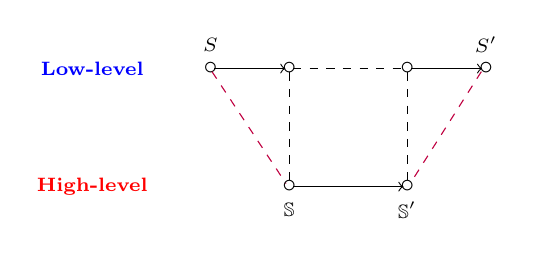
\begin{tikzpicture}[scale=1]
        \node(low-level) at (0, 1.5) {\bf \scriptsize \color{blue} Low-level};
        \node(lnode1) at (1.5, 1.5) {$\circ$};
        \node(lnode2) at (2.5, 1.5) {$\circ$};
        \node(lnode3) at (4, 1.5) {$\circ$};
        \node(lnode4) at (5, 1.5) {$\circ$};

        \draw[->] (1.55, 1.5) -- (2.45, 1.5);
        \draw[-,dashed] (2.55, 1.5) -- (3.95, 1.5);
        \draw[->] (4.05, 1.5) -- (4.95, 1.5);

        \node(linitState) at (1.5, 1.8) {\scriptsize $\state$};
        \node(lfinishState) at (5, 1.8) {\scriptsize $\state'$};

        %%%%%%%%%%%%%%%%%%%%%%%%%%%%%%%%%%%%%%%%%%%%%%%

        \draw[-,dashed, purple] (1.52, 1.46) -- (2.46, 0.04);
        \draw[-, dashed] (2.5, 1.45) -- (2.5, 0.05);
        \draw[-, dashed] (4, 1.45) -- (4, 0.05);
        \draw[-,dashed, purple] (4.94, 1.46) -- (4.05, 0.06);
        
        %%%%%%%%%%%%%%%%%%%%%%%%%%%%%%%%%%%%%%%%%%%%%%%

        \node(high-level) at (0, 0) {\bf \scriptsize \color{red} High-level};
        \node(hnode2) at (2.5, 0) {$\circ$};
        \node(hnode3) at (4, 0) {$\circ$};

        \draw[->] (2.55, 0) -- (3.95, 0);
        \node(hinitState) at (2.5, -0.3) {\scriptsize $\hpstate$};
        \node(hfinishState) at (4, -0.3) {\scriptsize $\hpstate'$};
    \end{tikzpicture}
    \caption{Logic Ensures State Relation Reestablished}
    \label{fig:Logic Ensures State Relation Reestablished}
    \vspace{-1em}
\end{figure}
% (\Fig{\ref{fig:Logic Ensures State Relation Reestablished}} gives a 
% more straightforward way to understand this restriction, and 
% we use the purple dashed line to represent this invariant). 
We define \INV{} to represent this invariant below formally: 
% our logic needs to make sure that 
% the state relation defined in 
% \Def{\ref{fig:State Relation between Low- and High-level Program State}}, 
% should be reestablished at the exit of function, shown as 
% \Fig{\ref{fig:Logic Ensures State Relation Reestablished}} 
% (the purple dashed line representing the state relation holding). 
% We define \INV{} below
% as an auxiliary definition and discuss it in two cases:
% shows 
% this requirements in a more straightforward way, 
% and we use the purple dashed line to represent the state relation holds. 
% We define the state relation between low- and high-level 
% program state in \Fig{\ref{fig:rel-wp}}. 
% \Fig{\ref{fig:Logic Ensures State Relation Reestablished}} shows that 
% our logic needs to make sure that 
% if the state relation holds at the entry of the function, then it 
% should be reestablished at the exit of function. 
% We use the purple dashed to represent the state relation holds in 
% \Fig{\ref{fig:Logic Ensures State Relation Reestablished}}. 
% either, (a) the specification belongs to context switch module, 
% the current thread $\thrdid$ will become a ready thread, and a 
% ready thread {\color{blue} $\thrdid'$} will become current thread after the execution 
% of the function; or, (2) the specification does not belong to context 
% switch, the execution of this function will not change the id 
% of the current thread. The primitive command $\primcom$ is also 
% required to be able to execute safely in \INV{}'s definition, 
% because the refinement relation between 
% the low- and high-level program is established under 
% the assumption that the high-level program is safe
% (defined as $\progsafe(\HProg)$)  
% as described in \Def{\ref{def:prim-correctness}}.
% $\INV{((\thrdid, \thrdid'), \primcom, \word, \args{\val})}$ 
% and $\INV{(\thrdid, \primcom, \word, \args{\val})}$ 
% are auxiliary definitions defined below:  
\[
    \small
    \begin{array}{l}
        % \INV{(\primdone, \args{\val})} \ \define \ 
        % \{
        % (\state, \hpstate, \primcom, \word) \sepline
        % \stateRel{\state}{\hpstate}
        % \land 
        % \arguments(\hpstate.\hthrdlocalst.\hRstate, \,  
        % \hpstate.\Mem, \args{\val})
        % \} \\
        % \\[-8pt]
        \INV{(\primcom, \args{\val})} \ \define \ 
        \{
            (\state, \hpstate, \primcom, \word) \sepline
            \colorbox{yellow!80}{\!$\stateRel{\state}{\hpstate}$\!}
            \land 
            \colorbox{yellow!80}
            {\!\!\!
                $\exists \, \hpstate'. \,
                \primMultiTrans
                    {(\primcom, \hpstate)}
                    {*}{(\primdone, \hpstate')}$ 
            \!\!\!} \\
            \hspace*{15.8em} 
            \land \
            \arguments(\hpstate.\hthrdlocalst.\hRstate, \,  
            \hpstate.\Mem, \args{\val})
        \}
    \end{array}
\]
The invariant consists of the state relation between low- and 
high-level program state 
(define as $\stateRel{\state}{\hpstate}$ in 
\Fig{\ref{fig:State Relation between Low- and High-level Program State}}), 
and the safe execution of the primitive command
($\primMultiTrans{}{*}{}$ means zero or one step). 
Including the safe execution of 
the primitive command is essential 
because we can get some knowledges of high-level program 
state from the safe execution of 
primitive command $\primcom$. 
For example, if $\INV{(\primsw(\nil), \nil)}$
holds, we can know that the location $\TaskNew$ 
must save a pointer pointing to a ready thread
in thread pool from the safe execution of primitive $\primsw$. 
% and we 
% can write them in the precondition of the specification 
% of the context switch routine. 
% Otherwise, 
% the execution of primtive $\primsw$ will not be safe. 
And we can know that the memory location $\TaskNew$ 
in low-level state also saves such pointer 
according to the state relation 
between low- and high-level program state. 
\[
    \small
    \begin{array}{l}
        \INV{(\primsw(\nil), \nil)} 
        \Longrightarrow \\ 
        \exists \, \thrdid, \hthrdlocalst. \, 
        (\hmsto{\TaskNew}{(\thrdid, 0)}) 
        \sepstar 
        (\astRdyCont{\thrdid}{\hthrdlocalst})
        \sepstar
        (\msto{\TaskNew}{(\thrdid, 0)})
        \sepstar \atrue
    \end{array}
\]
% {\small 
% \[
%     \INV{(\primsw(\nil), \word, \nil)} 
%     \Longrightarrow 
%     \exists \, \thrdid, \hthrdlocalst. \, 
%     \hmsto{\TaskNew}{(\thrdid, 0)} 
%     \sepstar 
%     (\astRdyCont{\thrdid}{\hthrdlocalst})
%     \sepstar \atrue
% \]
% } 
We introduce frame $\relastP_r$ for local reasoning, 
and it should be stable under the execution 
of the abstract assembly primitive 
(shown as $\Sta(\hprim(\args{\val}), \relastP_r)$)
defined below). 

{\small
\begin{multline*}
    \Sta(\hprim(\args{\val}), \relastP_r) 
    \define 
    \forall \, \state, \hpstate, \hpstate', \word. \\ 
    ((\asrtmodel{(\state, \hpstate, \hprim(\args{\val}), \word)}
        {\relastP_r\sepstar\atrue}) 
    \land
    \hprim(\args{\val})(\hpstate)(\hpstate'))\imp \\
    \asrtmodel{(\state, \hpstate', \primdone, \word)}
        {\relastP_r\sepstar\atrue} 
\end{multline*}
}
We show that our extended program logic is sufficient 
to prove the contextual refinement between 
a context switch routine written in SPARCv8
and $\primsw$ primitive 
in Appendix~\ref{appendix:ctxswitchproof}. 
% {\small 
% \begin{multline*}
% 	\forall \, \hpstate_c, \, \hpstate_c', \, \hpstate_r, 
% 	\word, \, \state, \, \relastP_r.  \\
% 	\primTrans{(\hprim(\args{\val}), \hpstate_c)}
% 		{(\primdone, \hpstate_c')} \, \land \, 
% 	\hpstate_c \perp \hpstate_r \, \land \, 
% 	\asrtmodel{(\state, \hpstate_r, \hprim(\args{\val}), \word)}
% 		{\relastP_r} \Longrightarrow \qquad  \qquad \\
% 	\exists \, \hpstate_r'. \, 
% 	\primTrans{(\hprim(\args{\val}), \hpstate_c \uplus \hpstate_r)}
% 		{(\primdone, \hpstate_c' \uplus \hpstate_r')} \, \land \, 
% 		\hpstate_c' \perp \hpstate_r' \, \land \, 
% 		\asrtmodel{(\state, \hpstate_r', \primdone, \word)}
% 			{\relastP_r}
% \end{multline*}
% }
% \vspace*{-1em}
\subsection{Logic Ensuring Contextual Refinement}
\label{subsec:logic-ensuring-ctxrefinement}

We give the semantics of \textbf{WfPrim} rule in 
\Def{\ref{def:wdprim-sem}}. 
% The meaning of 
% $\semWdPrim{\Cspec}{\asmimp}{\hprimset}$ is straightforward. 
It says that any high-level abstract assemly primitive 
in primitive set $\hprimset$ can 
establish a simulation relation with its low-level 
implementation in code heap $\asmimp$. We define this 
simulation relation in \Def{\ref{def:sim-impl-prim}}, 
which means that if there 
exists a relational state $(\state, \hpstate, \primcom, \word)$ 
satisfies the precondition $\relastP$, then we have 
the simulation 
$\simFunctionSt{\relastQ}{(\asmimp, \state, \lab{}, \lab{} + 4)}
    {i}{0}{(\primcom, \hpstate)}$ defined in 
\Def{\ref{def:sim-imp-prim-state}}. 

% The simulation 
% relation between implementation and its corresponding 
% abstract assembly primitive is defined in 
% \Def{\ref{def:sim-impl-prim}}, and means that if there 
% exists a relational state $(\state, \hpstate, \primcom, \word)$ 
% satisfies the precondition $\relastP$, then we have 
% the simulation 
% $\simFunctionSt{\relastQ}{(\asmimp, \state, \lab{}, \lab{} + 4)}
%     {i}{0}{(\primcom, \hpstate)}$ defined in 
% \Def{\ref{def:sim-imp-prim-state}}. 

\begin{definition}[Well-defined Primitive Set Semantics]
    \em
    \label{def:wdprim-sem}
    \small
    \[
        \begin{array}{l}
            \semWdPrim{\Cspec}{\asmimp}{\hprimset} 
            \, \define \, 
            \forall \, \lab{} \in \dom(\hprimset), \, 
            \lgvl. \ 
            \exists \, \hprim, \, \args{\val}, \,
            \relspecpre, \relspecpost.  \\
            \hspace*{5em}
            \wdSpec{\relspecpre}{\relspecpost} {\hprim} 
            	\, \land \, 
            	(\relspecpre \ \lgvl \Longrightarrow  
            	\safePrimAst{\, \hprim(\args{\val}) \,} 
                \sepstar \atrue) \\
            \hspace*{5em}
            \, \land \, 
            \simFunction{(\asmimp, \lab{})}
                {(\relspecpre \ \lgvl, \,
                    \relspecpost \ \lgvl)}
                {\hprim(\args{\val})}
            \\
            \\[-9pt]
            \hspace*{1em}
            \TYPE{where } \, 
            \hprimset(\lab{}) = \hprim, 
            \Cspec(\lab{}) = (\relspecpre, \relspecpost), \\
            \hspace*{5em}
            \TYPE{ and }
            \simFunction{(\asmimp, \lab{})}
                {(\relastP, \relastQ)}{\primcom}
            \TYPE{ is defined 
            \Def{\ref{def:sim-impl-prim}}}.
        \end{array}
        % \begin{array}{lcl}
        %     \semWdPrim{\Cspec}{\asmimp}{\hprimset}
        %     & \define & 
        %     \forall \, \lab{} \in \dom(\hprimset), \, 
        %     \lgvl. \ 
        %     \exists \, \hprim, \, \args{\val}, \,
        %     \relspecpre, \relspecpost.  \\
        %     \multicolumn{3}{l}
        %     {
        %     	\hspace*{5em}
        %     	\wdSpec{\relspecpre}{\relspecpost} {\hprim} 
        %     	\, \land \, 
        %     	(\relspecpre \ \lgvl \Longrightarrow  
        %     	\safePrimAst{\, \hprim(\args{\val}) \,} 
        %     	\sepstar \atrue)
        %     	\, \land \, 
        %     	\simFunction{(\asmimp, \lab{})}{\relspecpre \ \lgvl, \,
        %     		\relspecpost \ \lgvl}{\hprim(\args{\val})}
        %     }
        %     \\
        %     \\[-9pt]
        %     \multicolumn{3}{l}
        %     {
        %         \hspace*{3em}
        %         \TYPE{where } \, 
        %         \hprimset(\lab{}) = \hprim, 
        %         \Cspec(\lab{}) = (\relspecpre, \relspecpost), 
        %         \TYPE{ and }
        %         \simFunction{(\asmimp, \lab{})}{\relastP, \relastQ}{\primcom}
        %         \TYPE{ is defined 
        %         \Def{\ref{def:sim-impl-prim}}}. 
        %     }      
        % \end{array}
    \]
    % $\semWdPrim{\Cspec}{\asmimp}{\hprimset}$ holds, iff. 
    % for any $\lab{} \in \dom(\hprimset)$ and $\args{\val}$, 
    % there exists $\hprim, \, \lgvl, \, \relspecpre$ and 
    % $\relspecpost$, such that $\wdSpec{\relspecpre}{\relspecpost}{\hprim}$ 
    % and $\simFunction{(\asmimp, \lab{})}{\relspecpre \ \lgvl, \,
    %     \relspecpost \ \lgvl}{(\hprim(\args{\val}), \hpstate)}$ hold, 
    % where $\hprimset(\lab{}) = \hprim$, 
    % $\Cspec(\lab{}) = (\relspecpre, \relspecpost)$, and 
    % $\simFunction{(\asmimp, \lab{})}{\relastP, \relastQ}{\primcom}$
    % is defined in \Def{\ref{def:sim-impl-prim}}.
\end{definition}

\begin{definition}[Simulation for Implementation and Primitive]
    \em
    \label{def:sim-impl-prim}
    \small
    \[
        \begin{array}{l}
            \simFunction{(\asmimp, \lab{})}
                {(\relastP, \, \relastQ)}{\primcom}
            \ \define \ 
            \forall \, \state, \, \hpstate, \, \word. \,      
            \asrtmodel{(\state, \hpstate, \primcom, \word)}{\relastP}
            \Longrightarrow \\
            \hspace*{6em}
            \exists \, i \in \Index. \ 
            \simFunctionSt{\relastQ}{(\asmimp, \state, \lab{}, \lab{}+4)}
                {i}{0}{(\primcom, \hpstate)} \\
            \\[-9pt]
            \hspace*{1em}
            \text{where } 
            \simFunctionSt{\relastQ}{(\asmimp, \state, \pc, \npc)}
                {i}{k}{(\primcom, \hpstate)}
            \TYPE{ is defined in 
            \Def{\ref{def:sim-imp-prim-state}}}.
        \end{array}
        % \begin{array}{lcl}
        %     \simFunction{(\asmimp, \lab{})}{\relastP, \, \relastQ}{\primcom}
        %     & \define & 
        %     \forall \, \state, \, \hpstate, \, \word. \,      
        %     \asrtmodel{(\state, \hpstate, \primcom, \word)}{\relastP}
        %     \Longrightarrow \\
        %     & & \qquad
        %     \exists \, i \in \Index. \ 
        %     \simFunctionSt{\relastQ}{(\asmimp, \state, \lab{}, \lab{}+4)}
        %         {i}{0}{(\primcom, \hpstate)} \\
        %     \\[-9pt]
        %     \multicolumn{3}{l}
        %     {
        %         \hspace*{4em}
        %         \TYPE{where } 
        %         \simFunctionSt{\relastQ}{(\asmimp, \state, \pc, \npc)}
        %             {i}{k}{(\primcom, \hpstate)}
        %         \TYPE{ is defined in 
        %         \Def{\ref{def:sim-imp-prim-state}}}.      
        %     }    
        % \end{array}
    \]
    % $\simFunction{(\asmimp, \lab{})}{\relastP, \, \relastQ}{\primcom}$
    % holds, iff. for any $\state, \, \hpstate, \, \word$, if 
    % $\asrtmodel{(\state, \hpstate, \primcom, \word)}{\relastP}$ 
    % holds, then there exists $i \in \Index$, such that 
    % $\simFunctionSt{\relastQ}{(\asmimp, \state, \lab{}, \lab{}+4)}
    %     {i}{0}{(\primcom, \hpstate)}$ holds, 
    %     where $\simFunctionSt{\relastQ}{(\asmimp, \state, \pc, \npc)}
    %     {i}{k}{(\primcom, \hpstate)}$ is defined in 
    %     \Def{\ref{def:sim-imp-prim-state}}. 
\end{definition}

\begin{definition}
    \em
    \label{def:sim-imp-prim-state}
    Whenever
    $\simFunctionSt{\relastQ}{(\asmimp, \state, \pc, \npc)}{i}{k}{(\primcom, \hpstate)}$
    holds, we have the following holds : 
    \small
    \begin{enumerate}
        \item if $\asmimp(\pc) = \simplins$, then: 
            \begin{itemize}
                \item there exists $\state', \pc', \npc'$, 
                    such that \\
                    $\LGlobTrans{(\asmimp, \state, \pc, \npc)}{\empmsg\,}
                        {(\asmimp, \state', \pc', \npc')}$; 
                \item for any $\state', \pc', \npc'$, \\ 
                    if 
                    $\LGlobTrans{(\asmimp, \state, \pc, \npc)}{\empmsg\,}
                        {(\asmimp, \state', \pc', \npc')}$, then one of 
                        the following holds: 
                    \begin{enumerate}
                        \item $\exists \, j < i. \ 
                            \simFunctionSt{\relastQ}{(\asmimp, \state', \pc', \npc')}
                                {j}{k}{(\primcom, \hpstate)}$; 
                        \item there exists $\hpstate', \, j \in \Index$, 
                            such that \\
                            $\primTrans{(\primcom, \hpstate)}{(\primdone, \hpstate')}$ 
                            and \\
                            $\simFunctionSt{\relastQ}{(\asmimp, \state', \pc', \npc')}
                                {j}{k}{(\primdone, \hpstate')}$ holds; 
                    \end{enumerate}
            \end{itemize}
            \vspace{0.5em}
        
        \item if $\asmimp(\pc) = \call \ \lab{}$, then:
            \begin{itemize}
                \item there exists $\state', \, \pc', \, \npc'$, 
                 such that \\
                    $\LGlobMultiTrans{(\asmimp, \state, \pc, \npc)}
                        {\empmsg\,}{2}{(\asmimp, \state', \pc', \npc')}$; 
                \item for any $\state', \pc', \npc'$, \\ if 
                $\LGlobMultiTrans{(\asmimp, \state, \pc, \npc)}{\empmsg\,}
                    {2}{(\asmimp, \state', \pc', \npc')}$, then one of 
                    the following holds: 
                \begin{enumerate}
                    \item $\exists \, j < i. \ 
                        \simFunctionSt{\relastQ}{(\asmimp, \state', \pc', \npc')}
                            {j}{k+1}{(\primcom, \hpstate)}$; 
                    \item there exists $\hpstate', \, j \in \Index$, 
                        such that \\
                        $\primTrans{(\primcom, \hpstate)}{(\primdone, \hpstate')}$ 
                        and \\
                        $\simFunctionSt{\relastQ}{(\asmimp, \state', \pc', \npc')}
                            {j}{k+1}{(\primdone, \hpstate')}$ holds; 
                \end{enumerate}
            \end{itemize}
            \vspace{0.5em}
        
        \item if $\asmimp(\pc) = \retl{}$, then: 
            \begin{itemize}
                \item there exists $\state', \, \pc', \, \npc'$, 
                such that \\
                   $\LGlobMultiTrans{(\asmimp, \state, \pc, \npc)}
                       {\empmsg\,}{2}{(\asmimp, \state', \pc', \npc')}$;
                \item for any $\state', \pc', \npc'$, \\
                    if $\LGlobMultiTrans{(\asmimp, \state, \pc, \npc)}
                            {\empmsg\,}{2}{(\asmimp, \state', \pc', \npc')}$
                    then there exists $j \in \Index$, $\hpstate'$ and 
                    $\primcom'$, such that the following holds: 
                    \begin{enumerate}
                        \item either $j < i$, $\hpstate' = \hpstate$
                            and $\primcom' = \primcom$; or
                            $\primTrans{(\primcom, \hpstate)}{(\primcom', \hpstate')}$;
                        \item if $k = 0$, then there exists 
                        	$\word'$: 
                        	(where $\state'.\Rstate.\RFile(\reg{15})
                        	 = \lab{}$) \\
                            \hspace*{2em} 
                            $\asrtmodel{(\state', \hpstate', \primcom', \word')}
                                {\relastQ}$, 
                            $\primcom' = \primdone$, \\
                            \hspace*{2em}
                            $\pc' = \lab{}\!+\!8$, and 
                            $\npc' = \lab{}\!+\!12$; \\
                            else \\
                            \hspace*{2em}
                            $\simFunctionSt{\relastQ}{(\asmimp, \state', \pc', \npc')}
                                {j}{k-1}{(\primcom', \hpstate')}$.
                    \end{enumerate}
            \end{itemize}
        
%        	\item $\{ \asmimp(\pc), \, \asmimp(\npc) \}
%        		\in \{ \simplins, \, \call \ \lab{}, \, 
%        		\retl \}$
    \end{enumerate}
\end{definition}

The definition of simulation 
$\simFunctionSt{\relastQ}{(\asmimp, \state, \pc, \npc)}
    {i}{k}{(\primcom, \hpstate)}$ carries an index $i$, 
which is used to ensure the termination preserving, 
and the depth $k$ of function call. 
The simulation relation can not only make sure 
the safe execution of low-level SPARCv8 function, 
which is similar with the $\safe{}$ defined in 
\Def{\ref{def:safety}}, but also ensure the 
safe execution of the corresponding high-level abstract 
assembly primitive. Theorem~\ref{thm:logic soundness}, 
whose correctness can be derived from Lemmas 
\ref{lemma:Logic Ensures Simulation} 
and \ref{lemma:Simulation Implies Primitive Correctness}, 
shows the soundness of our logic, 
which means that the extended program logic can 
imply the contextual refinement between implementation 
$\asmimp$ and abstract assembly primitives $\hprimset$. 
% The correctness of logic soundness can be 
% achieved from Lemmas \ref{lemma:Logic Ensures Simulation} 
% and \ref{lemma:Simulation Implies Primitive Correctness}. 

\begin{lemma}[Logic Ensures Simulation]
    \em
    \label{lemma:Logic Ensures Simulation}
    \[
        \wfprim{\Cspec}{\asmimp}{\hprimset} \Longrightarrow 
        \semWdPrim{\Cspec}{\asmimp}{\hprimset}
    \]
\end{lemma}

\begin{lemma}[Simulation Implies Primitive Correctness]
    \em
    \label{lemma:Simulation Implies Primitive Correctness}
    \[
        \semWdPrim{\Cspec}{\asmimp}{\hprimset} 
        \Longrightarrow
        \asmimp \refine \hprimset
    \]
\end{lemma}

\begin{theorem}[Logic Soundness]
    \em
    \label{thm:logic soundness}
    \[
        \wfprim{\Cspec}{\asmimp}{\hprimset} \Longrightarrow
        \asmimp \refine \hprimset
    \]
\end{theorem}
  \section{Related Work and Conclusion}
\label{sec:conclusion}

There has been much work on assembly or
machine code verification. Most of them
do not support function calls or simply
treat function calls in the continuation-passing
style where return addresses are viewed as first
class code pointers~\cite{PCC,FPCC,TAL,TALx86,Yu03ESOP,xcap,cflogic}.
SCAP~\cite{Feng06pldi} supports assembly code verification
with various stack-based control abstractions, including
function call and return. We follow the same idea here.
However, SCAP gives a syntactic-based soundness proof
by establishing the preservation of the syntactic judgment,
which makes it difficult to interact with other modules
verified in different logic. Since our goal is to
verify inline assembly and link the verified code
with the verified C programs, we give a direct-style
semantic model of the logic judgments. And it allows us 
to extend our program logic to support verifying 
contextual refinement without meet much challenges. 
Also SCAP
is based on a simplified subset of assembly instructions,
while our work is focused on a realistically modeled
subset of \sparc{} instructions.

In terms of the support of realistic instruction sets,
previous work on proof-carrying code (PCC) and
typed assembly language (TAL) mostly supports subsets of
x86.
Myreen's work \cite{arm-veri} presents a framework for
ARM verification based on a realistic model
(but it doesn't support function call and return).

As part of the Foundational Proof-Carrying Code (FPCC)
project~\cite{FPCC},
Tan and Appel present a program logic $\mathcal{L}_c$
for reasoning about control flow in assembly code~\cite{cflogic}.
Although $\mathcal{L}_c$ is implemented on top of SPARC machine
language, the underlying logic is a type system instead
of a full-blown program logic for functional correctness.
It reasons about functions in the continuation-passing
style. Also 
handling SPARC features such as delayed writes or delayed
control transfers is not the focus of $\mathcal{L}_c$.
%They also reason about functions in the continuation-passing
%style.
There has been work on mechanized semantics of the SPARCv8 ISA.
%Here are already some works for SPARCv8 ISA formalization.
\etal{Hou}~\cite{sparcv8-formalization-Isabelle} model the SPARCv8 ISA
in Isabelle/HOL, and test their formal model against 
LENON3 simulation board \cite{LEON3}, 
which is a synthesisable VHDL model of a 32-bit processor 
compliant with the SPARCv8 architecture, 
through more than 100,000 instruction instances.   
\etal{Wang}~\cite{sparc-formalization} formalize its semantics in Coq.
%However, both of their works give no program logic.
Our operational semantics of SPARCv8 follows \etal{Wang}~\cite{sparc-formalization}.
%\etal{Wang}~\cite{sparc-formalization}
%formalize the SPARCv8 ISA in Coq but give
%no program logic. Our operational
%semantics of SPARCv8 follows their work. 
But \etal{Wang} do not validate their formalization against actual 
hardware, we remain it as a future work. 

\etal{Ni}~\cite{ctxm} verify a context switch module of 19 lines
in x86 code to show case the support of embedded
code pointers (ECP) in XCAP~\cite{xcap}. The context switch
module we verify comes from a practical OS kernel,
which is more realistic and consists of more than 250 lines
of assembly code, but our logic (\textbf{CALL} rule) 
does not really support the switch of return pointers,   
which requires further extension like OCAP~\cite{FengTLDI07}. 
Our focus is to verify the
code manages the register windows, and the function calls made internally. 
We address this problem of calling context switch routine in 
another way in our work, such that we can use the extended 
program logic to verify the contextual refinement between 
context switch routine and $\primsw{}$ primitive. 
The method of verifying context switch primitive in our work is 
inspired by the approach used by \etal{Guo}~\cite{ctxmGuo}
that protects the TCBs through abstraction, but the state 
relation between low- and high-level program state in our work is more 
sophisticated than theirs, because of some specific mechanisms, 
like register windows, in SPARCv8. 
They also do not develop a general program 
logic for refinement verification of the assembly.  
Our extended program logic is based on the relational program logic, 
which has already been well used 
successfully in the refinement verification 
of C-style language \cite{Xu16cav,liang13pldi,liang14lics}.  

Yang and Hawblitzel~\cite{YangPLDI10} verify Verve, an x86 
implementation of an experimental operating system. Verve has two 
levels, the high-level TAL code and the low-level ``Nucleus'' 
that provides primitive access to hardware and memory. 
The Nucleus code is verified automatically using the Z3 SMT solver,
while the goal of our work is to generate machine checkable proofs.
Another key difference is the use of different ISAs. Here
we give details to verify specific features of SPARCv8 programs.

There have been many techniques and tools proposed for automated
program verification (\eg~\cite{SymbolicExecutionSpLogic,Smallfoot}).
It is possible to adapt them to verify SPARCv8 code.
We propose a new program logic and do the verification in Coq mainly
because the work is part of a big project for a fully certified OS 
kernel for aerospace crafts whose inline assembly is written in 
SPARCv8. We already have a program logic implemented in Coq for 
C programs, which allows us to verify C code with Coq proofs. 
Therefore we want to have a program logic for SPARCv8 so that 
it can be linked with the
logic for C and can generate machine-checkable Coq proofs too.
That said, many of the automated verification techniques can
be applied to reduce the manual efforts to write Coq proofs,
which we would like to study in the future work. 
We have already shown that it's possible to apply some 
Coq tactics based on separation logic \cite{practical-tactics} 
in our work.  


% %Most of our code verification works are done by hand now.
% %\etal{Berdine}~\cite{SymbolicExecutionSpLogic}\cite{Smallfoot} describe a
% %method for proving Hoare triples by a form of symbolic execution,
% %in order to achieve automatical reasoning. Their symbolic execution algorithm
% %works by proof-search using operational and rearrangement rules.
% %%Our current work consider less about automatical reasoning,
% %%but it's possible to do much effort on it in the future.
% %The operational rules in Berdine's work are similar with
% %traditional Hoare logic rules with some certain restrictions on pre- and post-condition,
% %and their rearrangement rules can be viewed as some derived rules from the basic ones.
% %So, in order to use their algorithm to achieve automatic reasoning of SPARCv8 code,
% %we have to design a Hoare-style program logic for SPARCv8 code firstly,
% %which is the aim of our work.
% %%With a Hoare-style program logic for SPARCv8 code,
% %%their algorithm can be implemented as a Coq tactic.
% %Although, our current work consider less about automatical reasoning,
% %it's possible to extend it and their algorithm can be implemented as a Coq tactic
% %based on our Hoare-style program logic for SPARCv8 code in the future.
% %
% %\indent
% %There are many impressive pioneering works
% %that focus on machine code verification.
% %Projects on proof-carrying code (PCC) \cite{PCC, FPCC}
% %and typed assembly language (TAL) \cite{TAL, TALx86}
% %evoke interests in low-level code verification.
% %They aim to find a method to address safety properties
% %of assembly code by automatic type-checking.
% %Generating proofs automatically is difficult in many times.
% %So, the work \cite{Yu03ESOP} of \etal{Yu} provides the CAP framework
% %to support a Hoare-logic style reasoning for assembly code.
% %However, works on PCC, TAL and CAP only focus on
% %the safety properties of assembly code.
% %
% %\indent
% %Certifying function call/return in assembly code is difficult,
% %because assembly codes are usually lacking structure.
% %\etal{Feng} develop SCAP framework \cite{Feng06pldi}
% %for verification of assembly code with all kinds of
% %stack-based control abstraction,
% %including function call/return.
% %Our method to handle function call/return is inspired by SCAP.
% %%
% %However, most works on CAP, including SCAP,
% %are based on a simply abstract machine model
% %and establish soundness following the syntactic approach
% %of proving type sound.
% %And they also do not give the frame rule for local verification.
% %Myreen's work \cite{arm-veri} presents a framework for
% %ARM verification based on a realistic model
% %and can state the functional behavior of ARM program,
% %but doesn't support function call/return verification.
% %
% %work \cite{cflogic}
% %which is a part of Foundational Proof-Carrying Code (FPCC) \cite{FPCC}
% %presents a program logic about reasoning unstructured control flow
% %in machine-language program.
% %Although their logic is implemented
% %on the top of SPARC machine language and
% %provides fine-grained composition rules to compose program segment,
% %the main target of their work is not to design a program logic
% %specially for SPARC code.
% %They do not consider the main features of SPARC in their logic
% %and still treat function call and return as the first-class function.
% %
% %
% %\indent
% %Following the CAP framework,
% %\etal{Ni} present XCAP \cite{xcap} to solve
% %embedded code pointers (ECPs) problem in assembly code level,
% %and \etal{Feng} extend the basic CAP to handler
% %concurrent multi-threaded assembly code verification.
% %Our current work is not support ECPs
% %and concurrency verifications \cite{Feng05ICFP, Feng08pldi, Yu04ICFP}.
% %So, these work can be the complementaries in our future work.
% %
% %\indent
% %The existent works about SPARC are less.
% %\etal{Wang} \cite{sparc-formalization}
% %formalize the SPARCv8 ISA in Coq.
% %Their work does not develop a program logic
% %and uses the operational semantics for code reasoning directly.
% %Tan and Apple's work \cite{cflogic}
% %which is a part of Foundational Proof-Carrying Code (FPCC) \cite{FPCC}
% %presents a program logic about reasoning unstructured control flow
% %in machine-language program.
% %Although their logic is implemented
% %on the top of SPARC machine language and
% %provides fine-grained composition rules to compose program segment,
% %the main target of their work is not to design a program logic
% %specially for SPARC code.
% %They do not consider the main features of SPARC in their logic
% %and still treat function call and return as the first-class function.
% %
% %\indent
% %Context switch module is an important component in OS kernel.
% %There exists many works to verify a context switch module
% %that \etal{Ni} have used the XCAP framework
% %to certify a machine context management in x86 \cite{ctxm}.
% %However, the programs they proved are implemented by them
% %and context switch module is only 19 lines in their work.
% %We prove a realistic context switch module
% %which is more complex and considers more details
% %and cases for actual execution.
% %Although we does not consider ECPs problem
% %which XCAP can handler well,
% %it does not influence the context switch module that we verified
% %to link with other modules,
% %because it's a function and our logic supports
% %function call/return verification.

\paragraph{\textbf{Conclusion.}}
We present a program logic for \sparc.
Our logic is based on a realistic semantics
model and supports main features of \sparc,
including delayed control transfer, delayed writes,
and register windows.
We have applied the program logic to verify
the main body of the context switch routine
in a realistic embedded OS kernel. 
And we also extend the program logic to support 
refinement verification. 
Our current work can only handle
sequential \sparc{} program verification and 
do not consider interrupt in machine model.  
We will extend it for concurrency verification 
and finish the step {\color{blue} \textcircled{1}} shown in
\Fig{\ref{fig:idea to establish contextual refinement}}
that the compilant can ensure the behaviors 
of the Pseudo-SPARCv8 code calling abstraction assembly 
primitives in intermediate level refines 
the behaviors of 
the client C code calling abstract assembly primitives 
in source level in the future. 
% %and accurate models of \sparc{} program,
% %and supports module, local, function call/return
% %and main features of \sparc{} verification.
% %We also give a semantic approach for soundness establishing
% %and prove the soundness of our logic.
% %We finally apply it to verify a context switch module
% %which has been used in an actual embedded OS kernel.
% % Our current work can only handle
% % sequential \sparc{} program verification for partial correctness.
% % We will extend it for concurrency
% % and refinement verification in the future. Also
% % we would like to link the verified inline assembly
% % with verified C code for whole system
% % verification.


  \bibliographystyle{unsrt}{
    \footnotesize
    \itemsep=-3pt plus.2pt minus.2pt
    \baselineskip=13pt plus.2pt minus.2pt
    \bibliography{refs}}
\end{multicols}

\appendix
  \renewcommand {\thefigure} {A\arabic{figure}}
  \setcounter{figure}{0}
  \section{More about High-level Instructions Execution}
\label{appendix:more-about-high-level-insExec}

We give some supplements about the execution of high-level instructions. 
As we have explained in \Sec{\ref{subsec:High-level Pseudo-SPARCv8 Language}}, 
the register windows and delayed buffer in pyhsical SPARCv8 program state 
are omitted in high-level Pseudo-SPARCv8 program state. So, we do not define  
state transtion rules for instructions $\csave{}$, $\crestore{}$, $\rd{}$, 
and $\cwr{}$. The instruction transition rules for the rest of instructions, like  
$\ld{}$ and $\cadd{}$, have no much difference with the rules in pyhical SPARCv8 program. 
\begin{figure}[!h]
    \centering
    \[
        \begin{array}{c}
            \infer
            {
                \hexeci{(\ld \ \aexp \ \reg{d}, ((\hRfile, \block, \hWstk), \Mem))}
                    {((\hRfile', \block, \hWstk), \Mem)}
            }
            {
                \evalR{\aexp}{\hRfile} = \loc \quad \ \ 
                \Mem(\loc) = \val \quad \ \ 
                \hRfile' = \hRfile\hRegUpd{ \reg{d} \rightsquigarrow \val } 
            } \\
            \\[-5pt]
            \infer
            {
                \hexeci{(\cadd \ \reg{s}, \oexp, \reg{d}, ((\hRfile, \block, \hWstk), \Mem))}
                    {((\hRfile', \block, \hWstk), \Mem)}
            }
            {
                \hRfile(\reg{s}) = \val_1 \quad \ \ 
                \evalR{\oexp}{\hRfile} = \val_2 \quad \ \ 
                \reg{d} = \dom(\hRfile) \quad \ \ 
                \hRfile' = \hRfile\hRegUpd{ \reg{d} \rightsquigarrow \val }
            }
        \end{array}
    \]
    \caption{Transition rules for instructions \ld{} and \cadd{} in high-level}
    \label{fig:Transition rules for instructions ld and add in high-level}
\end{figure}

We show the state transition rules for instructions \ld{} and \cadd{} 
in high-level in \Fig{\ref{fig:Transition rules for instructions ld and add in high-level}}. 
The register file updating operation is defined formally below : 
\[
    \hRfile\hRegUpd{\hrn \rightsquigarrow \val} \ \define \ 
    \hRfile\{ \hrn \rightsquigarrow \val \} \quad \ \ 
    \text{where } \, 
    \hrn \notin \{ \spreg, \fpreg \}
\] 
According to the definition, we can find that updating the register $\spreg$ 
(alias of $\reg{14}$), which is used to point to the top of the current 
stack frame, and $\fpreg$ (alias of $\reg{14}$), which is used to point to 
the top of the previous stack frame is not allowed. Only the execution of instructions  
$\Psave$, which is used to allocate a new stack frame, 
and $\Prestore{}$, which is used to free the current stack frame, can modify them. 
The evaluation of the opand and address expression in high-level is defined formally 
below : 
\[
    \begin{array}{ll}
        \begin{array}{lcl}
            \evalR{\oexp}{\hRfile} & \define &
                \left\{
                    \begin{array}{ll}
                        R(r) &\quad \cif \ \oexp = r \\
                        \\[-8pt]
                        w &\quad \cif \ \oexp = \word, \\
                        & \quad \quad -4096 \leq \word \leq 4095 \\
                        \\[-8pt]
                        \perp &\quad \otherwise
                    \end{array}
                \right.
        \end{array} & \quad
        \begin{array}{lcl}
            \evalR{\aexp}{\hRfile} & \define &
                \left\{
                    \begin{array}{ll}
                        \evalR{\oexp}{\hRfile} &\quad \cif \ \aexp = \oexp \\
                        \\[-8pt]

                        \val_1 \!+\! \val_2
                        &\quad \cif \ \aexp = \regr \!+\! \oexp,\
                        \hRfile(\regr) \!=\! \val_1 \\
                        & \quad \quad \tand \ \evalR{\oexp}{\hRfile} = \val_2 \\

                        \\[-8pt]
                        \perp &\quad \otherwise
                    \end{array}
                \right.
        \end{array}
    \end{array}
\]

The `` $\Psave \ \word$ " can be viewed as a macro of 
`` $\csave{} \ \spreg, -\word, \spreg$ ", and `` $\Prestore{}$ " 
can be viewed as a marco of `` $\crestore{} \ \greg{0}, \greg{0}, \greg{0}$ ". 
\begin{figure}[h]
    \centering
    \[
        \begin{array}{c|c}
            \begin{array}{lcl}
                \csave{} & \quad & \spreg, -128, \spreg \\
                \cadd{} & & \ireg{0}, \ireg{1}, \ireg{0} \\
                \ret{} \\
                \crestore{} & & \greg{0}, \greg{0}, \greg{0} \\
                & (a)
            \end{array} \qquad & \qquad 
            \begin{array}{lcl}
                \Psave & \quad & 128 \\
                \cadd{} & & \ireg{0}, \ireg{1}, \ireg{0} \\
                \ret{} \\
                \Prestore{} & & \\
                & (b)
            \end{array}
        \end{array}
    \]
    \caption{Realistic SPARCv8 Code and Pseudo-SPARCv8 Code}
    \label{fig:Realistic SPARCv8 Code and Pseudo-SPARCv8 Code}
\end{figure}

\Fig{\ref{fig:Realistic SPARCv8 Code and Pseudo-SPARCv8 Code}} 
gives a simple comparision with the realistic SPARCv8 code 
and our Pseudo SPARCv8 code in high-level. 
\Fig{\ref{fig:Realistic SPARCv8 Code and Pseudo-SPARCv8 Code}} 
(a) is the realistic SPARCv8 code. 
It uses instruction `` $\csave{} \, \spreg, -128, \spreg$ " 
to store the caller's context and allocate a new stack frame 
size 128 bytes for the current procedure, and use instruction
`` $\crestore{} \ \greg{0}, \greg{0}, \greg{0}$ " to restore 
the caller's context at the exitance of the current procedure. 
\Fig{\ref{fig:Realistic SPARCv8 Code and Pseudo-SPARCv8 Code}} (b) is 
the same function in Pseudo-SPARCv8 code, 
and we can find that the instructions that 
is responsible for saving and restoring the context of caller
is replaced by `` $\Psave \ 128$ " and `` $\Prestore$ ". 
  \section{More about Low-level Language}
\label{sec:more-llang}

The machine states and syntax low-level SPARCv8 language 
(defined in \Fig{\ref{fig:machine-state-syntax-low-level-sparc}}) 
are taken from the model of SPARCv8 defined in 
\Fig{\ref{fig:Machine States and Language for SPARC Code}}. 
So, we omit some definitions, like RegName and DelayCycle, 
which are same as ones defined in 
\Fig{\ref{fig:Machine States and Language for SPARC Code}} here.

\begin{figure}[!h]
    \centering
    \vspace{-2em}
    \[
        \begin{array}{rcclcrccl}
            \text{(LProg)} & \ \prog \ & \define & (\code, \state, \pc, \npc) 
            & \quad \ \ &
            \text{(LState)} & \ \state \ & \define & (\Mem, \Rstate, \DBuf) 
            \\
            \text{(LRstate)} & \ \Rstate \ & \define & (\RFile, \Wstack) & &
            \text{(LRegFile)} & \RFile & \define & 
                \text{RegName} \rightharpoonup \text{Val} \\
            \text{(LFrmList)} & \Wstack & \define & \nil \sepline \fm \stCons \Wstack 
            & &
            \text{(LFrame)} & \fm & \define & [\val_0, \dots, \val_7]
            \\
            \text{(DBuf)} & \DBuf & \define & \nil \sepline (\tick, X, \val) & & 
            \text{(LMsg)} & \ \lmsg \ & \define & \empmsg \sepline \outEvt{\val}
        \end{array}
    \]
    \vspace{-1em}
    \caption{Machine States and Syntax for Low-level SPARCv8 Language}
    \label{fig:machine-state-syntax-low-level-sparc}
    \vspace{-1em}
\end{figure}
The low-level program $\prog$ is a tuple including the code heap $\code$, 
low-level program state $\state$, program counter $\pc$ and $\npc$. The 
code heap $\code$ is defined in \Fig{\ref{fig:syntax-of-concur-pseudo-sparc}}. 
The low-level program state $\state$ uses the block-based memory model $\Mem$, 
which is the same as the high-level program. The low-level message does not need 
$\callEvt{\lab{}, \args{\val}}$, because the low-level program does not call 
abstract assembly primitive, but call its corresponding implementation, which 
is a function. 

\begin{figure}[!t]
    \centering
    \small
    \subfigure[Low-level Program Transition]{
        \begin{minipage}[b]{1\textwidth}
        \[
            \begin{array}{c}
                \infer
                {
                    \LGlobTrans{(\code, (\Mem, (\RFile, \Wstack), \DBuf), \pc, \npc)}
                        { \ \lmsg \ }
                        {(\code, (\Mem, (\RFile'', \Wstack'), \DBuf''))}
                }
                {
                    \begin{array}{l}
                        \Dstep{(\RFile, \Wstack)}{(\RFile', \Wstack')} \\
                        \llocalstep{\code}
                            {((\Mem, (\RFile', \Wstack), \DBuf'), \pc, \npc)}
                            { \ \lmsg \ }
                            {(\Mem', (\RFile'', \Wstack'), \DBuf'')}
                    \end{array}
                }
            \end{array}
        \]
        \vspace{0.2em}
        \end{minipage}
    }

    \subfigure[Low-level Control Transfer Instruction Transition]{
        \begin{minipage}[b]{1\textwidth}
        \[
            \begin{array}{c}
                \infer
                {
                    \llocalstep{\code}
                        {((\Mem, \Rstate, \DBuf), \pc, \npc)}
                        { \ \empmsg \ }
                        {((\Mem', \Rstate', \DBuf'), \npc, \npc + 4)}
                }
                {
                    \code(\pc) = \simplins{} \quad \ \ 
                    \lexeci{(\simplins{}, (\Mem, \Rstate, \DBuf))}
                        {(\Mem', \Rstate', \DBuf')}
                } \\
                \\
                \infer
                {
                    \llocalstep{\code}
                        {((\Mem, (\RFile, \Wstack), \DBuf), \pc, \npc)}
                        { \ \empmsg \ }
                        {((\Mem, (\RFile, \Wstack), \DBuf), \npc, \lab{})}
                }
                {
                    \code(\pc) = \jmp{} \ \aexp \quad \ \ 
                    \evalR{\aexp}{\RFile} = \lab{}
                } \\
                \\
                \infer
                {
                    \llocalstep{\code}
                        {((\Mem, (\RFile, \Wstack), \DBuf), \pc, \npc)}
                        { \ \empmsg \ }
                        {((\Mem, (\RFile\{ \reg{15} \rightsquigarrow \pc \}, 
                            \Wstack), \DBuf), \npc, \lab{})}
                }
                {
                    \code(\pc) = \call \ \lab{} \quad \ \ 
                    \reg{15} \in \dom(\RFile)
                } \\
                \\
                \infer
                {
                    \llocalstep{\code}
                        {((\Mem, (\RFile, \Wstack), \DBuf), \pc, \npc)}
                        { \ \empmsg \ }
                        {((\Mem, (\RFile, \Wstack), \DBuf), \npc, \lab{} + 8)}
                }
                {
                    \code(\pc) = \retl{} \quad \ \ \RFile(\reg{15}) = \lab{}
                } \\
                \\
                \infer
                {
                    \llocalstep{\code}
                        {((\Mem, (\RFile, \Wstack), \DBuf), \pc, \npc)}
                        { \, \outRN(\val) \, }
                        {((\Mem, (\RFile, \Wstack), \DBuf), \npc, \npc + 4)}
                }
                {
                    \code(\pc) = \cprint \quad \ \ \RFile(\oreg{0}) = \val
                } \\
                \\
                \infer
                {
                    \llocalstep{\code}
                        {((\Mem, (\RFile, \Wstack), \DBuf), \pc, \npc)}
                        { \, \empmsg \, }
                        {((\Mem', (\RFile', \Wstack'), \DBuf), \pc, \npc)}
                }
                {
                    \code(\pc) = \Psave \ \word \quad \ \ 
                    \decwin{(\RFile, \Wstack)} = \undef \quad \ \ 
                    \winOverFlow{(\Mem, \RFile, \Wstack)}
                        {(\Mem', \RFile', \Wstack')}
                } \\
                \\
                \infer
                {
                    \llocalstep{\code}
                        {((\Mem, (\RFile, \Wstack), \DBuf), \pc, \npc)}
                        { \, \empmsg \, }
                        {((\Mem', (\RFile', \Wstack'), \DBuf), \pc, \npc)}
                }
                {
                    \code(\pc) = \Prestore \quad \ \ 
                    \incwin{(\RFile, \Wstack)} = \undef \quad \ \ 
                    \winUnderFlow{(\Mem, \RFile, \Wstack)}
                        {(\Mem', \RFile', \Wstack')}
                }
            \end{array}
        \]
        \vspace{0.2em}
        \end{minipage}
    }

    \subfigure[Low-level Instruction Transition]
    {
        \begin{minipage}[b]{1\textwidth}
        \[
            \begin{array}{c}
                \infer
                {
                    \lexeci{(\Psave \ \word, (\Mem, (\RFile, \Wstack), \DBuf))}
                        {(\Mem', (\RFile', \Wstack'), \DBuf)}
                }
                {
                    \malloc(\Mem, \block, 0, \word) = \Mem' \quad \ \ 
                    \decwin{(\RFile, \Wstack)} = (\RFile', \Wstack') \quad \ \ 
                    \RFile'' = \RFile'\{ \spreg \rightsquigarrow (\block, 0) \}
                } \\
                \\
                \infer
                {
                    \lexeci{(\Prestore, (\Mem, (\RFile, \Wstack), \DBuf))}
                        {(\Mem', (\RFile'', \Wstack'), \DBuf)}
                }
                {
                    \mfree(\block, \Mem) = \Mem' \quad \ \ 
                    \incwin{(\RFile, \Wstack)} = (\RFile', \Wstack') 
                } \\
                \\
                \infer
                {
                    \lexeci{(\csave{} \ \reg{s} \ \oexp \ \reg{d}, 
                        (\Mem, (\RFile, \Wstack), \DBuf))}
                        {(\Mem', (\RFile', \Wstack'), \DBuf)}
                }
                {
                    \decwin{(\RFile, \Wstack)} = (\RFile'', \Wstack') \quad \ \ 
                    \evalR{\oexp}{\RFile} = \val \quad \ \ 
                    \RFile'' = \RFile'\{ \reg{d} \rightsquigarrow 
                        \RFile(\reg{s}) + \val \}
                } \\
                \\
                \infer
                {
                    \lexeci{(\crestore{} \ \reg{s} \ \oexp \ \reg{d}, 
                        (\Mem, (\RFile, \Wstack), \DBuf))}
                        {(\Mem, (\RFile'', \Wstack'), \DBuf')}
                }
                {
                    \incwin{(\RFile, \Wstack)} = (\RFile', \Wstack') \quad \ \
                    \evalR{\oexp}{\RFile} = \val \quad \ \ 
                    \RFile'' = \RFile'\{ \reg{d} \rightsquigarrow 
                        \RFile(\reg{s}) + \val \}
                }
            \end{array}
        \]
        \vspace{0.2em}
        \end{minipage}
    }

    \subfigure[Low-level Expression Semantics]
	{
		\begin{minipage}[b]{1\linewidth}
            $$
            \begin{array}{ll}
                \begin{array}{lcl}
                    \evalR{\oexp}{R} & \define &
                    \left\{
                        \begin{array}{ll}
                            R(r) &\quad \cif \ \oexp = r \\
                            \\[-8pt]
                            w &\quad \cif \ \oexp = (\block, \word') \, \textbf{or} \, 
                                \oexp = \word, \\
                            & \quad \quad -4096 \leq \word \leq 4095 \\
                            \\[-8pt]
                            \perp &\quad \otherwise
                        \end{array}
                    \right.
                \end{array} & \quad
                \begin{array}{lcl}
                    \evalR{\aexp}{R} & \define &
                    \left\{
                        \begin{array}{ll}
                            \evalR{\oexp}{R} &\quad \cif \ \aexp = \oexp \\
                            \\[-8pt]

                            \val_1 \!+\! \val_2
                              &\quad \cif \ \aexp = \regr \!+\! \oexp,\
                              R(\regr) \!=\! \val_1 \\
                            & \quad \quad \tand \ 
                                \evalR{\oexp}{\RFile} = \val_2 \\

                            \\[-8pt]
                            \perp &\quad \otherwise
                        \end{array}
                    \right.
                \end{array}
            \end{array}
            $$
			\vspace{0.3cm}
		\end{minipage}	
	}
    \caption{Selected operational semantics rules for low-level program}
    \label{fig:selected-opsem-low-level-program}
    \vspace{-1em}
\end{figure} 

\begin{figure}[!t]
    \centering
    \small
    \[
        \begin{array}{l}
            \fresh(\block, \Mem) \ \define \ \forall \ \word. \, (\block, \word) \notin \dom(\Mem)
            \\
            \\[-5pt]
            \malloc(\Mem, \block, \word_l, \word_h) = \Mem' \ \define \ 
            (\Mem' = \Mem \, \land \, \word_l = \word_h) \, \lor \, 
            \\
            \qquad\qquad
            (\Mem' = \Mem 
                        \{ (\block, \word_l) \rightsquigarrow \notCare, \dots, 
                            (\block, \word_h - 1) \rightsquigarrow \notCare \}
            \, \land \, \fresh(\block, \Mem) \, \land \, 
            \word_l < \word_h) 
            \\
            \\[-5pt]
            \mfree(\block, \Mem) = \Mem' \ \define \ 
            \forall \, \block' \neq \block, \word'. \ 
            \Mem'(\block', \word') = \Mem(\block', \word') \, \land \, 
            \nexists \, \word. \ (\block, \word) \in \dom(\Mem)
        \end{array}
    \]
    \caption{Auxiliary Definitions for Memory Operation}
    \label{fig:Auxiliary Definitions for Memory Operation}
    \vspace{-0.5em}
\end{figure}

\begin{figure}[!t]
    \centering
    \[
		\begin{array}{c}
			\infer
			{
				\winOverFlow{(\mem, (\RFile, \Wstack))}{(\mem', (\RFile', \Wstack))}
			}
			{
                \begin{array}{c}
                    \Wstack = \Wstack_1 \lstApp \fm_1 \lstApp \fm_2 \lstApp 
                        \fm_3 \lstApp \fm_4 \quad  \ \ \fm_1[6] = (\block, 0) \\
                    \RFile(\regwim) = 2^n \quad \ \ 
                    \{ (\block, 0), \dots, (\block, 15) \} \subseteq \dom(\mem) \quad \ \ 
                    \RFile' = \RFile''\{ \regwim \rightsquigarrow 2^{\nextcwp{(n)}} \} \\
                    \mem' = \mem\{ \Array{(\block, 0), \dots, (\block, 7)} \rightsquigarrow \fm_2 \}
						\{ \Array{(\block, 8), \dots, (\block, 15)} \rightsquigarrow \fm_3 \}
					% \decwin{(\decwin{(\RFile, \Wstack)})} = (\RFile_0, \Wstack_0) \quad \ \ 
					% \RFile_0(\spreg) = (\block_0, 0) \quad \ \ \RFile(\regwim) = 2^n \\
					% \{ (\block_0, 0), \dots, (\block_0, 15) \} \subseteq \dom(\mem) \\
					% \mem' = \mem\{ \Array{(\block_0, 0), \dots, (\block_0, 7)} \rightsquigarrow 
					% 	\RFile_0([\localRN]) \}
					% 	\{ \Array{(\block_0, 8), \dots, (\block_0, 15)} \rightsquigarrow 
					% 		\RFile_0([\inRN]) \} \\
					% \incwin{(\incwin(\RFile_0, \Wstack_0))} = (\RFile'', \Wstack') \quad \ \ 
					% \RFile' = \RFile''\{ \regwim \rightsquigarrow 2^{\nextcwp{(n)}} \}
				\end{array}
			} \\
			\\[-5pt]
			\infer
			{
				\winUnderFlow{(\mem, (\RFile, \Wstack))}{(\mem, (\RFile', \Wstack'))}
			}
			{
                \begin{array}{c}
                    \Wstack = \fm_1 \stCons \fm_2 \stCons \Wstack'' \quad \ \ 
                    \RFile(\reg{30}) = (\block, 0) \quad \ \ \RFile(\regwim) = 2^n \\ 
                    \{
						\Array{(\block, 0), \dots, (\block, 7)} \rightsquigarrow \fm_1', 
						\Array{(\block, 8), \dots, (\block, 15)} \rightsquigarrow \fm_2'
                    \} \subseteq \mem' \\
                    \RFile' = \RFile''\{\regwim \rightsquigarrow 2^{\prevcwp{(n)}}\} \quad \ \ 
                    \Wstack' = \fm_1' \stCons \fm_2' \stCons \Wstack'' 
					% \incwin{(\RFile, \Wstack)} = (\RFile_0, \Wstack_0) \quad \ \ 
					% \RFile_0(\spreg) = (\block_0, 0) \quad \ \ 
					% \RFile(\regwim) = 2^n \\
					% \{
					% 	\Array{(\block_0, 0), \dots, (\block_0, 7)} \rightsquigarrow \fm_1, 
					% 	\Array{(\block_0, 8), \dots, (\block_0, 15)} \rightsquigarrow \fm_2
					% \} \subseteq \mem \\
					% \RFile_0' = \RFile_0\{ \localRN \rightsquigarrow \fm_1, 
					% 	\inRN \rightsquigarrow \fm_2 \} \\
					% \decwin{(\RFile_0', \Wstack_0)} = (\RFile'', \Wstack') \quad \ \ 
					% \RFile' = \RFile''\{\regwim \rightsquigarrow 2^{\prevcwp{(n)}}\}
				\end{array}
			}
		\end{array}
    \]
    \caption{Windows Over- and UnderFlow}
    \label{fig:Windows Over- and UnderFlow}
    \vspace{-0.5em}
\end{figure}

\paragraph{\bf Operational Semantics for Low-level Code.} 
The operational semantics for low-level program is defined in 
\Fig{\ref{fig:selected-opsem-low-level-program}}. Most of the 
state transition rules are taken from 
\Fig{\ref{Selected Operational Semantics}}. Here, we use 
``$\lexeci{(\simplins{}, \notCare)}{\notCare}$" to represent 
the step for simple instruction $\simplins{}$.

The execution of instruction $\Psave$ is discussed in divided 
into two cases : (1) if we can successfully set the next register 
window as the current one (represented as 
$\decwin{(\RFile, \Wstack)} = (\RFile', \Wstack')$),   
a new stack frame in memory will be allocated
(shown as $\malloc(\Mem, \block, 0, \word) = \Mem'$); 
(2) if we can't set the next register window as the current 
one (represented as $\decwin{(\RFile, \Wstack)} = \undef$), 
a windows overflow trap will be triggered, and we redo the 
instruction $\Psave$. The execution of instruction $\Prestore$ 
does the reverse. Here, we use ``$\winOverFlow{\notCare}{\notCare}$" 
to represent the state transition caused by window overflow trap and 
use ``$\winUnderFlow{\notCare}{\notCare}$" to represent the state 
transition caused by window underflow trap. Their formal definitions 
are shown in \Fig{\ref{fig:Windows Over- and UnderFlow}}. 
  \section{More about State Relation Between Low- and High-level Program}
\label{sec:more-staterel}

After introducing the definitions of low- and high-level program, 
we establish the state relation between low- and high-level program 
in this section. Establishing their state relation is not a trivial 
task, because there are two major differences low- and high-level 
program states. \textbf{First}, all the procedures' contexts of 
a specific thread are saved in high-level frame list $\hWstk$. 
However, for low-level program, part of the contexts are saved in 
register windows (modeled as low-level frame list $\Wstack$), the 
other part of the contexts are saved in corresponding stack frame 
in memory, because the number of register windows is limited; 
\textbf{Second}, the high-level concurrent Pseudo-SPARCv8 program 
is multithreaded, but the low-level SPARCv8 program does not have 
the concept of thread pool. 

\begin{figure}[!t]
    \centering
    \small
    \[
        \begin{array}{c}
            \infer
            {
                \stkRel{(\block, \nil, \emptyset)}{\nil}
            }
            {} \qquad \quad
            \infer
            {
                \stkRel{(\block, \nil, \Mem_K)}{(\block, \fm_1, \fm_2) \stCons \hWstk}
            }
            {
                \Mem_K = \framMem{(\block, \fm_1, \fm_2)} \uplus \Mem_K' 
                \quad \ \ \fm_2[6] = (\block', 0) \quad \ \  
                \stkRel{(\block', \nil, \Mem_K')}{\hWstk}
            } \\
            \\
            \infer
            {
                \stkRel{(\block,
                	\fm_1 \stCons \fm_2 \stCons \Wstack, \Mem_K)}
                    {(\block, \fm_1', \fm_2') \stCons \hWstk}
            }
            {
                \fm_1 = \fm_1' \quad \ \ \fm_2 = \fm_2' \quad \ \  
                \Mem_K = \framMem{(\block, \notCare, \notCare)} \uplus \Mem_K'
                \quad \ \ 
                \fm_2[6] = (\block', 0) \quad \ \ 
                \stkRel{(\block', \Wstack, \Mem_K')}{\hWstk}
            }
        \end{array}
    \]
    \caption{Relation for low- and high-level FrameList}
    \label{fig:relation-low-high-level-framelist}
\end{figure}

\paragraph{\bf Relation for low- and high-level FrameList.} 
The relation between low- and high-level frame list is defined in 
\Fig{\ref{fig:relation-low-high-level-framelist}}. We represent 
this relation as form 
``$\stkRel{(\block, \Wstack, \Mem_K)}{\hWstk}$", 
The tuple of $\block$, 
$\Wstack$ and $\Mem_K$ is the state of stack in low-level program, 
because, in the low-level program, part of the produces' contexts are 
saved in frame list $\Wstack$, which can also be understand as a 
prefix the whole frame list describe in assertion $\stackAstP{\notCare}{\Wstack}$, 
the other part of the contexts are saved in corresponding frame list 
represent as $\Mem_K$. The high-level frame list $\hWstk$ represents the 
state of stack in high-level program. 
\Fig{\ref{fig:Abstraction of Register Windows and Memory}} gives a 
more intuition understanding of this relation. Here, some part of 
the contexts $\Wstack$ (the pink part in the left side of the 
\Fig{\ref{fig:Abstraction of Register Windows and Memory}}) 
are saved in register windows, and the other part of contexts 
$\Mem_K$ (the green part in the left side of the 
\Fig{\ref{fig:Abstraction of Register Windows and Memory}}) are 
saved in stack frame in memory. However, in high-level state, 
they are abstracted as list named high-level frame list $\hWstk$. 
\begin{figure}[!t]
    \centering
    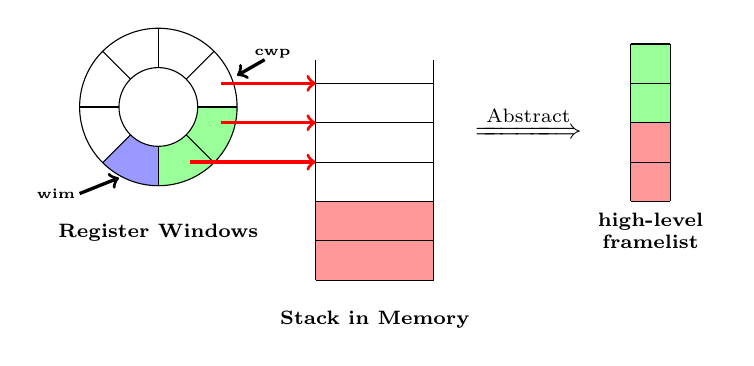
\begin{tikzpicture}
        \fill[green!40!white] (0,0) -- (0,-1cm) arc (-90:0:1cm) -- (0,0);
        \fill[blue!40!white] (0,0) -- (0,-1cm) arc (-90:-135:1cm) -- (0,0);
        % \fill[yellow!80!white] (0,0) -- (0,-1cm) arc (-90:-135:1cm) -- (0,0);
        % \fill[blue!40!white] (0,0) -- (-1,0cm) arc (-180:-135:1cm) -- (0,0);
        \draw (0, 0) -- (90:1cm);
        \draw (0, 0) -- (45:1cm);
        \draw (0, 0) -- (0:1cm);
        \draw (0, 0) -- (-45:1cm);
        \draw (0, 0) -- (-90:1cm);
        \draw (0, 0) -- (-135:1cm);
        \draw (0, 0) -- (-180:1cm);
        \draw (0, 0) -- (135:1cm);
        \fill[white] (0, 0) circle (0.5cm);
        \draw (0, 0) circle (1cm);
        \draw (0, 0) circle (0.5cm);
        % \draw[very thick, blue] (0, -0.3) -- (0, -1.2);
        % \draw[very thick, blue] (0, -0.32) -- (0.1, -0.32);
        % \draw[very thick, blue] (0, -1.18) -- (0.1, -1.18);
        \node(wim) at (-1.3, -1.1) {\tiny \bf wim};
        \draw[->, very thick] (-1, -1.1) -- (-0.5, -0.9);

        % \node(wim) at (-1.7, -0.7) {\tiny \bf wim};
        % \draw[->, very thick] (-1.5, -0.6) -- (-1, -0.4);
        

        \node(cwp) at (1.45, 0.67) {\tiny \bf cwp};
        \draw[->, very thick] (1.35, 0.6) -- (1, 0.4);

        \node(regwin) at (0, -1.6) {\scriptsize \bf Register Windows};

        %%%%%%%%%%%%%%%%%%%%%%%%%%%%%%%%%%%%%%%%%%%%%%%%%%%%%%

        \fill[red!40!white] (2, -1.2) rectangle (3.5, -1.7);
        \fill[red!40!white] (2, -1.7) rectangle (3.5, -2.2);

        \draw[-] (2, 0.6) -- (2, -2.2);
        \draw[-] (3.5, 0.6) -- (3.5, -2.2);
        
        \draw[-] (2, 0.3) -- (3.5, 0.3);
        \draw[-] (2, -0.2) -- (3.5, -0.2);
        \draw[-] (2, -0.7) -- (3.5, -0.7);
        \draw[-] (2, -1.2) -- (3.5, -1.2);
        \draw[-] (2, -1.7) -- (3.5, -1.7);
        \draw[-] (2, -2.2) -- (3.5, -2.2);

        \node(stkfm) at (2.75, -2.7) {\scriptsize \bf Stack in Memory};

        %%%%%%%%%%%%%%%%%%%%%%%%%%%%%%%%%%%%%%%%%%%%%%%%%%%%%%%

        \draw[->, very thick, red] (0.8, 0.3) -- (2, 0.3);
        \draw[->, very thick, red] (0.8, -0.2) -- (2, -0.2);
        \draw[->, very thick, red] (0.4, -0.7) -- (2, -0.7);

        %%%%%%%%%%%%%%%%%%%%%%%%%%%%%%%%%%%%%%%%%%%%%%%%%%%%%%

        \node(abstract) at (4.7, -0.2) {$\xLongrightarrow{\text{Abstract}}$};

        %%%%%%%%%%%%%%%%%%%%%%%%%%%%%%%%%%%%%%%%%%%%%%%%%%%%%%

        \fill[green!40!white] (6, 0.8) rectangle (6.5, 0.3);
        \fill[green!40!white] (6, 0.3) rectangle (6.5, -0.2);
        \fill[red!40!white] (6, -0.2) rectangle (6.5, -0.7);
        \fill[red!40!white] (6, -0.7) rectangle (6.5, -1.2);

        \draw[-] (6, 0.8) -- (6, -1.2);
        \draw[-] (6.5, 0.8) -- (6.5, -1.2);

        \draw[-] (6, 0.8) -- (6.5, 0.8);
        \draw[-] (6, 0.3) -- (6.5, 0.3);
        \draw[-] (6, -0.2) -- (6.5, -0.2);
        \draw[-] (6, -0.7) -- (6.5, -0.7);
        \draw[-] (6, -1.2) -- (6.5, -1.2);

        \node(hfrmlist) at (6.25, -1.6) 
            {
                \scriptsize \bf
                $
                \begin{array}{c}
                    \text{high-level} \\
                    \text{framelist}
                \end{array}
                $
            };
    \end{tikzpicture} 
    \caption{Abstraction of Register Windows and Memory}
    \label{fig:Abstraction of Register Windows and Memory}
    \vspace{-0.5em}
\end{figure}

As shown in \Fig{\ref{fig:relation-low-high-level-framelist}}, if 
the low-level frame list $\Wstack$ is $\nil$ and the memory is $\emptyset$, 
and the high-level frame list $\hWstk$ is $\nil$, it means there is no 
context stored. If the frame list is $\nil$ but the high-level frame list 
is $(\block, \fm_1, \fm_2) \stCons \hWstk$, it means that the contexts 
$\fm_1$ and $\fm_2$ are saved in stack frame in memory, whose block identifier 
is $\block$. Here, we use ``$\framMem{(\block, \fm_1, \fm_2)}$" defined below to 
represent the part of memory saving $\fm_1$ and $\fm_2$. This memory contains 
only one block $\block$.  
\[
    \begin{array}{lll}
        \framMem{(\block, \fm_1, \fm_2)} & \define & 
        \{ (\block, 0) \rightsquigarrow \val_0, 
            (\block, 4) \rightsquigarrow \val_1, \dots, 
            (\block, 28) \rightsquigarrow \val_7 \} \\
        & & \quad \ \ \uplus
        \{
            (\block, 32) \rightsquigarrow \val_0', 
            (\block, 36) \rightsquigarrow \val_1', \dots,
            (\block, 60) \rightsquigarrow \val_7'   
        \} \\
        \\[-8pt]
        & 
        \multicolumn{2}{l}
        {
            \text{where} \  
            \fm_1 = \Array{\val_0, \dots, \val_7}, \,  
            \fm_2 = \Array{\val_0', \dots, \val_7'}. 
        }
    \end{array}
\]
If the frame list is $\fm_1 \stCons \fm_2 \stCons \Wstack$ 
and the high-level frame list is $(\block', \fm_1', \fm_2') \stCons \hWstk$, 
it means that the contexts $\fm_1$ and $\fm_2$ have not 
been saved in block $\block'$. So, we require the contexts 
$\fm_1$ and $\fm_2$ saved in low-level frame list and 
the $\fm_1'$ and $\fm_2'$ saved in high-level frame list 
are equal. The block $\block'$ used to save $\fm_1$ and $\fm_2$ 
has not been used yet, so we don't care about its contents. 

\paragraph{\bf Relation for ThreadPool and low-level Memory.} 
In high-level program, the thread local state of each thread 
is saved in a thread pool $\thrdpool$. However, in low-level 
program, the local state of each thread is saved in memory 
(TCB and stack). For example, in \Sec{\ref{sec:ctxswitch}}, 
we introduce that the execution of the context switch module
will save the register state of current thread into its 
TCB and stack in memory. So, the thread pool in high-level 
program can be viewed as an abstraction of low-level memory 
used to store the contexts of threads. 

\begin{figure}[!t]
    \centering
    \[
        \begin{array}{lcl}
            \ctxfm(\RFile, \Wstack) & \define & 
            \left\{
            \begin{array}{ll}
                \Wstack_1 & \quad \cif \
                \RFile(\regcwp) = \cwp, \, 
                \RFile(\regwim) = 2^{n}, \, 
                \regcwp \neq n, \\
                & \qquad
                \Wstack = \Wstack_1 \lstApp \Wstack_2, \, 
                0 \leq \cwp, n \leq N, \, 
                | \Wstack_1 | = 2 \times 
                    {(N + n - \cwp - 1)}\modOP{N} \\
                \\[-8pt]
                \perp & \quad \otherwise
            \end{array} 
            \right. \\
            \\
            \Rinj{\RFile}{\hRfile} & \define & 
            (\forall \, i \in \{ 0, \dots, 31 \}. \, 
                \RFile(\reg{i}) = \hRfile(\reg{i}))
                \, \land \, 
                (\forall \, \sr. \, \exists \, \word. \  
                \RFile(\sr) = \word) \\
            & & \quad \, \land \, 
            \RFile(\regn) = \hRfile(\regn) \, \land \, 
            \RFile(\regz) = \hRfile(\regz) \, \land \, 
            \RFile(\regc) = \hRfile(\regc) \, \land \, 
            \RFile(\regv) = \hRfile(\regv) \\
        \end{array}
    \]
    \[
        \begin{array}{c}
            \\[-5pt]
            \infer
            {
                \curStRel{(\Mem_c, (\RFile, \Wstack))}
                    {(\thrdid, ((\hRfile, \block, \hWstk), \pc, \npc))}
            }
            {
                \begin{array}{c}
                    \Mem_c = \Mem_{\text{ctx}} \uplus \Mem_K 
                    \quad \ \ 
                    \dom(\Mem_{\text{ctx}}) = \DomCtx{(\thrdid, \block)}
                    \quad \ \ 
                    \RFile(\spreg) = (\block, 0) 
                    \\
                    \ctxfm(\RFile, \Wstack) = \Wstack' \quad \ \ 
                    \RFile(\fpreg) = (\block', 0) \quad \ \ 
                    \stkRel{(\block', \Wstack', \Mem_K)}{\hWstk} 
                    \quad \ \ 
                    \Rinj{\RFile}{\hRfile} 
%                    \quad \ \ 
%                    \hRfile(\spreg) = (\block, 0)
                \end{array}
            } \\
            \\
            \infer
            {
                \rdyStRel{\Mem_1 \uplus \Mem_2}{\thrdpool_1 \uplus \thrdpool_2}
            }
            {
                \rdyStRel{\Mem_1}{\thrdpool_1} \quad \ \ 
                \rdyStRel{\Mem_2}{\thrdpool_2}
            } \qquad \quad
            \infer
            {
                \rdyStRel{\Mem}{\{ \thrdid \rightsquigarrow \hthrdlocalst \}}
            }
            {
                \restoreCtx{\Mem}{\thrdid}{\Rstate} \quad \ \ 
                \curStRel{(\Mem, \Rstate)}{(\thrdid, \hthrdlocalst)}
            }
        \end{array}
    \]
    \caption{Relation for Thread Pool and low-level Memory}
    \label{fig:rel-thrdpool-mem}
    \vspace{-1em}
\end{figure}

We define the relation between high-level thread pool and 
the memory used to save context in \Fig{\ref{fig:rel-thrdpool-mem}} formally. We use 
``$\curStRel{(\Mem_c, (\RFile, \Wstack))}
{(\thrdid, ((\hRfile, \block, \hWstk), \pc, \npc))}$" 
to represent the relation between the thread local states of 
{\it current thread} of low- and high-level program. 
The memory $\Mem_c$ owned the current thread $\thrdid$ can be 
splitted into two parts $\Mem_{\text{ctx}}$ and $\Mem_{\text{K}}$. The 
$\Mem_{\text{ctx}}$ are use the register file, whose domain is represented as 
$\DomCtx{(\thrdid, \block)}$. It takes two arguments : the identifier $\thrdid$ 
of the current thread and the block $\block$ of the stack frame at the top of the stack. 
Because the context switch module may save the register file in TCB and 
the stack frame of the current procedure. The other part of the memory $\Mem_K$ 
is used to save the contexts of the previous procedures, which is abstracted 
as $\hWstk$ in high-level program. We define $\Rinj{\RFile}{\hRfile}$ to 
represent the relation between the register file $\RFile$ in low-level and 
$\hRfile$ in high-level program. The operation $\ctxfm(\RFile, \Wstack)$ is 
used to exact the prefix $\Wstack_1$ of the frame list $\Wstack$, which saves 
the contexts of the previous procedures. Suppoing the value of the $\regcwp$ 
is $\cwp$, meaning that the id of the current window is $\cwp$, 
and the value of the $\regwim$ is $2^n$, meaning the id $n$ register window 
is invalid. According to the introduction in \Fig{\ref{subsec:syntax}}, 
we usually set a window invalid to avoid over- and underflow of the 
register windows. So, we known that register windows id from $(\cwp + 1)\modOP{N}$ 
to $(n - 1 + N)\modOP{N}$ save the contexts of the previous procedures. 
So, we extract the contents $\Wstack_1$ of them from the whole frame list $\Wstack$. 

We define ``$\rdyStRel{\Mem}{\{ \thrdid \rightsquigarrow \hthrdlocalst \}}$" 
to represent the relation between the thread local states of 
{\it ready thread} of low- and high-level program. The operation 
``$\restoreCtx{\Mem}{\thrdid}{\Rstate}$" means that we can restore the 
register state $\Rstate$ from memory $\Mem$. When the context of the 
ready thread has been restored, we can establish a relation 
``$\curStRel{(\mem, \Rstate)}{(\thrdid, \hthrdlocalst)}$" 
between low- and high-level thread local states of thread $\thrdid$. 
Here, we don't represent the definitions of $\DomCtx{(\thrdid, \block)}$ 
and $\restoreCtx{\Mem}{\thrdid}{\Rstate}$ here, because their definitions 
are based on the implementation of the context switch routine in 
OS kernel. And the soundness of our extended program logic does not 
rely on their concrete definition. 

\paragraph{\bf Relation for Whole Program State. } 
Finally, we introduce the state relation for whole program states between 
low- and high-level program below : 
\[
    \infer
    {
        \stateRel{(\Mem, \Rstate, \DBuf)}
            {(\thrdpool, \thrdid, \hthrdlocalst, \Mem')}
    }
    {
        \begin{array}{c}
            \Mem = \Mem_c \uplus \Mem_T \uplus 
                \{ \TaskCur \rightsquigarrow (\thrdid, 0) \}
                \uplus \Mem' \\
            \curStRel{(\Mem_c, \Rstate)}{(\thrdid, \hthrdlocalst)}
            \quad \ \ 
            \rdyStRel{\Mem_T}{\thrdpool \backslash \{ \thrdid \}}
            \quad \ \ 
            \DBuf = \nil
        \end{array}
    }
\]
  \section{Application of Extended Program Logic : Verifying a Simplified Version of Context Switch Routine}
\newcounter{lnum}
\setcounter{lnum}{1}
\newcommand{\llnum}{\thelnum\addtocounter{lnum}{1}}
\label{appendix:ctxswitchproof}

\begin{figure}[!h]
    \small
    \centering
    \[ 
        \begin{array}{lll}
            \multicolumn{3}{l}
                {
                    \quad \texttt{SwitchEntry}:
                    % \quad \lab{\texttt{switch}}: 
                } \\
            \\[-9pt]
            \llnum \quad \ \  
            & 
            \multicolumn{2}{l}
            {
                /* \text{codes save the \inRN{} and \localRN{}
                registers of current window into stack frame} */
            } \\
            % \llnum 
            % & \nop{} \\
            \llnum 
            & \sett & \TaskCur, \lreg{1} \\
            \llnum 
            & \ld & [\lreg{1}], \lreg{1} \\
            % \llnum 
            % & \cadd{} & \lreg{1}, \texttt{CONTEXT}\_\texttt{OFFSET}, \lreg{1} \\
            \llnum
            & \call{} & \texttt{reg}\_\texttt{save} \\
            \llnum
            & \nop{} \\
            \llnum
            & \mov{} & \regcwp, \greg{4} \\
            \llnum
            & \rd{} & \regwim, \greg{7} \\
            \llnum
            & \sett & 1, \greg{6} \\
            \llnum & \sll & \greg{6}, \greg{4}, \greg{4} \\
            \\[-5pt]
            \multicolumn{3}{l}
                {
                    \quad \texttt{Save}\_\texttt{Usedwindow}: 
                } \\
            \llnum & \sll & \greg{4}, 1, \greg{5} \\
            \llnum & \srl & \greg{5}, (\OSWINDOWs - 1), \greg{4} \\
            \llnum & \cor{} & \greg{4}, \greg{5}, \greg{4} \\
            \llnum & \andcc{} & \greg{4}, \greg{7}, \greg{0} \\
            \llnum & \bne & \texttt{Switch}\_\texttt{NewContext} \\
            \llnum & \nop{} \\
            \llnum & \crestore{} & \greg{0}, \greg{0}, \greg{0} \\
            \\[-9pt]
            \llnum & 
            \multicolumn{2}{l}
            {
                /* \text{codes save the \inRN{} and \localRN{}
                registers of current window into stack frame} */
            } \\
            \\[-9pt]
            % \call{} & \texttt{window}\_\texttt{save} \\
            \llnum & \nop{} \\
            \llnum & \jmp{} & \texttt{Save}\_\texttt{Usedwindow} \\
            \llnum & \nop{} \\
            \\[-5pt]
            \multicolumn{3}{l}
                {
                    \quad \texttt{Switch}\_\texttt{NewContext}: 
                } \\
            \llnum & \sett & \TaskCur, \lreg{0} \\
            \llnum & \sett & \TaskNew, \lreg{1} \\
            \llnum & \ld & [\lreg{1}], \lreg{1} \\
            \llnum & \st{} & \lreg{1}, [\lreg{0}] \\
            % \llnum & \cadd{} & \oreg{1}, \texttt{CONTEXT}\_\texttt{OFFSET}, \lreg{1} \\
            \llnum & \call{} & \texttt{reg}\_\texttt{restore} \\
            \llnum & \nop{} \\
            % \llnum & \call{} & \texttt{window}\_\texttt{restore} \\
            \\[-9pt]
            \llnum & 
            \multicolumn{2}{l}
            {
                /* \text{codes restore the \inRN{} and \localRN{}
                registers of current window from stack frame} */
            } \\
            \\[-9pt]
            \llnum & \nop{} \\
            \llnum & \retl{} \\
            \llnum & \nop{}
        \end{array}
    \]
    \caption{Main function of context switch routine}
    \label{fig:Main function of context switch routine}
\end{figure}

In this section, we give a simplified version of context switch routine in 
\Fig{\ref{fig:Main function of context switch routine}}. It reserves the 
main functionalities of the context switch routine introduced in 
\Sec{\ref{sec:ctxswitch}}, \eg saving the contexts of currrent thread 
and restoring the new one. We omit some details like judging whether the 
current thread is a valid thread. We give a simple introduction to the 
function shown in \Fig{\ref{fig:Main function of context switch routine}}, 
and show how to verify its correctness by applying our extended program 
logic for SPARCv8. 

\subsection{Simplified Context Switch Routine}

At the entrance of the context switch rountine shown in
\Fig{\ref{fig:Main function of context switch routine}}, we first 
% call an internal function \texttt{window}\_\texttt{save} to 
save the \localRN{} and \inRN{} registers into the stack in memory, 
and this part of the code is shown in 
\Fig{\ref{fig:code for saving and restoring local and in}}(a). 
Then, as shown from line 2 to 6, we call the \regsave{}  
to store the \outRN{} and \globalRN{} registers into the TCB 
of the current thread. As for the line 6 to 9, we get the identity of 
the current register window and the value of the \regwim{}. 
The block \SaveUsedWin{} (from line 10 to 20) saves the register windows 
(except the current one) into the stack of the current task in memory. 
It checks whether the previous window is valid. If it's valid, it 
uses the instruction $\crestore{}$ to set the previous window as the 
current one, and save its contents (\localRN{} and \inRN{} registers)
into stack in memory, then check the previous one continuously. 
The block \SwitchNewTask{} is responsible 
for restoring the context of the new task. From line 21 to 24, it 
sets the new task as the current one. Then, it calls function 
\texttt{reg}\_\texttt{restore} (at line 25)
to restore the $\outRN$ and $\globalRN$ 
registers from the new task's TCB, and restores the  
$\localRN$ and $\inRN$ registers from the new task's stack in memory. 
The code about restoring the $\localRN$ and $\inRN$ registers of 
the new task from memory is shown in 
\Fig{\ref{fig:code for saving and restoring local and in}}(b). 
The implementations of internal functions
\texttt{reg}\_\texttt{save} and \texttt{reg}\_\texttt{restore} 
are omitted here because these two functions are taken 
from the OS kernal we verified and we can't show these part 
of codes according to confidentiality agreement, but we show 
their specifications in \Fig{\ref{fig:Specifications of Internal Functions}}.

\subsection{Specification of the Simplified Context Switch Routine}

First, we define the abstract assembly primitive $\primsw$, which is 
already introduced in the \Sec{\ref{subsec:High-level Pseudo-SPARCv8 Language}}. 
{
    \small
    $$
    \begin{array}{lcl}
        \primsw & \define & 
        \lambda \, \args{\val}, \hpstate, \hpstate'. \ 
        \exists \, \thrdid'. \ 
        \Mem(\TaskNew) = (\thrdid', 0) \, \land \, 
        \thrdpool(\thrdid') = 
            (\hRstate', \pc', \npc') \\ 
        & & \hspace*{8em} \land \, 
        \thrdpool' = \thrdpool\{ \thrdid \rightsquigarrow 
        (\hRstate, \pc, \npc) \}
        \, \land \, \thrdid \neq \thrdid'
        \, \land \, \args{\val} = \nil \\
        \\[-8pt] 
        \multicolumn{3}{l}
        {
        	\hspace*{1.8em}
            \text{where } \, 
            \hpstate = 
                (\thrdpool, \thrdid, (\hRstate, \pc, \npc), \Mem), \, 
            \tid \in \dom(\thrdpool), \,
            \hpstate' = 
            (\thrdpool', \thrdid', 
            	(\hRstate', \lab{} + 8, \lab{} + 12), \Mem), \lab{} = \hRstate'.\hRfile(\reg{15}). 
%            \lab{} = \hRstate'.\hRfile(\reg{15}). 
            % \,
            % \AftExt(\hRstate, \pc, \npc) \define 
            % (\hRstate, \hRstate.\hRfile(\reg{15}) + 8, 
            %     \hRstate.\hRfile(\reg{15}) + 12)
        }
    \end{array}
    $$
}
Then we show the specification of the simplified context switch routine below, and some auxiliary 
definitions used in specification can be found in \Fig{\ref{def:aux-def-spec}}: 
{
    \small
    \[
        \begin{array}{lcl}
            \Apre(\thrdid_c, \thrdid_n, \env, \nst, \hthrdlocalst_c, \hthrdlocalst_n) 
            & \define & 
            \Env{\env} \sepstar
            (\relmsto{\TaskNew}{(\thrdid_n, 0)} \, \land \, \thrdid_c \neq \thrdid_n) \sepstar 
            \metricAst{10} \sepstar \\
            & & \quad 
            \RelCurT{\thrdid_c}{\notCare}{\env}{\hthrdlocalst_c} \sepstar 
            \RelRdyT{\thrdid_n}{\nst}{\hthrdlocalst_n} \sepstar 
            \safePrimAst{\, \primsw(\nil) \,} \\
            \\[-5pt]
            \Apost(\thrdid_c, \thrdid_n, \env, \nst, \hthrdlocalst_c, \hthrdlocalst_n)
            & \define & \exists \, \env', \hthrdlocalst'. \, \Env{\env'} 
            \sepstar (\relmsto{\TaskNew}{(\thrdid_n, 0)} \, \land \, \thrdid_c \neq \thrdid_n) 
            \sepstar \\
            & & 
            \quad 
            \RelCurT{\thrdid_n}{\nst}{\env'}{\hthrdlocalst'} \sepstar 
            \RelRdyT{\thrdid_c}{\pEnv{\env}}{\hthrdlocalst_c} \sepstar 
            \safePrimAst{\, \primdone \,}  
        \end{array}
    \]
} 

\begin{figure}[!t]
    \centering
    \vspace*{-0.5em}
    \small
    \[
        \begin{array}{l}
            \hspace*{-0.15em}
            \begin{array}{lcl}
                \RelStkFm{\block}{\fm_1}{\fm_2} & \define & 
                (\relmsto{(\block, 0)}{\fm_1[0]}) \sepstar \dots \sepstar 
                (\relmsto{(\block, 28)}{\fm_1[7]}) \\
                & & \quad \sepstar 
                (\relmsto{(\block, 32)}{\fm_2[0]}) \sepstar 
                \dots \sepstar
                (\relmsto{(\block, 60)}{\fm_2[7]})
            \end{array} \\
            \\[-5pt]
            \hspace*{-0.15em}
            \begin{array}{lcl}
                \RelStk{\block}{\Wstack}{\hWstk} & \define & 
                \left\{
                    \begin{array}{ll}
                        \RelStkFm{\block}{\notCare}{\notCare} \sepstar
                        \RelStk{\block'}{\Wstack'}{\hWstk'} & 
                            \quad \cif \  
                            \fm_2[6] = (\block', 0), \, \Wstack = \fm_1 \stCons \fm_2 \stCons \Wstack' \\
                            & \quad \ \ \hWstk = (\block, \fm_1, \fm_2) \stCons \hWstk' \\
                            \\[-8pt]
                        \RelStkFm{\block}{\fm_1}{\fm_2} \sepstar 
                        \RelStk{\block'}{\Wstack'}{\hWstk'} & 
                            \quad \cif \ 
                            \fm_2[6] = (\block', 0), \, \Wstack = \nil \\
                            & \quad \ \ \hWstk = (\block, \fm_1, \fm_2) \stCons \hWstk' \\
                            \\[-8pt]
                        \empAst & \quad \cif \ \Wstack = \nil, \hWstk = \nil \\
                            \\[-8pt]
                        \afalse & \quad \otherwise
                    \end{array}
                \right. 
            \end{array} \\
            \\[-5pt]
            \rRegs \ \define \ \regst{\asr_0}{\notCare} \sepstar \dots 
                        \regst{\asr_{31}}{\notCare} \sepstar \regst{\regY}{\notCare} \\
            \\[-5pt]
            \LRegs{\RFile} \ \define \ \regst{\globalRN}{\RFile(\globalRN)} \sepstar 
            \regst{\outRN}{\RFile(\outRN)} \sepstar \regst{\localRN}{\RFile(\localRN)} 
            \sepstar \regst{\inRN}{\RFile(\inRN)} \sepstar \\
            \hspace*{7em} \regst{\regn}{\RFile(\regn)} \sepstar 
            \regst{\regz}{\RFile(\regz)} \sepstar \regst{\regc}{\RFile(\regz)} 
            \sepstar \regst{\regv}{\RFile(\regv)} \sepstar \rRegs
            \\
            \\[-5pt]
            % \HRegs{\hRfile} \ \define \ \hregsto{\globalRN}{\hRfile(\globalRN)} \sepstar
            % \hregsto{\outRN}{\RFile(\outRN)} \sepstar \hregsto{\localRN}{\hRfile(\localRN)} 
            % \sepstar \hregsto{\inRN}{\hRfile(\inRN)} \\
            % \hspace*{7em} \hregsto{\regn}{\hRfile(\regn)} \sepstar 
            % \hregsto{\regz}{\hRfile(\regz)} \sepstar \hregsto{\regc}{\hRfile(\regz)} 
            % \sepstar \hregsto{\regv}{\hRfile(\regv)} \\
            % \\[-5pt]
            \wfwin{\RFile}{\Wstack} \ \define \ 
            (\stackAstP{\RFile(\regcwp)}{\Wstack} \sepstar 
                \regst{\regwim}{\RFile(\regwim)}) 
            \, \land \, \ctxfm(\RFile, \Wstack)
            \\
            \\[-5pt]
            \hspace*{-0.15em}
            \begin{array}{lll}
                \relcontext{\thrdid}{\block}{\nst} & \define & 
                (\relmsto{(\thrdid, \ofsGOne)}{\nst(\greg{0})}) 
                \sepstar \, \dots \, \sepstar
                (\relmsto{(\thrdid, \ofsGEig)}{\nst(\greg{7})}) \\
                & & 
                \sepstar
                (\relmsto{(\thrdid, \ofsOOne)}{\nst(\oreg{0})}) 
                \sepstar \, \dots \, \sepstar
                (\relmsto{(\thrdid, \ofsOEig)}{\nst(\oreg{7})}) \\
                & & 
                \sepstar 
                (\relmsto{(\thrdid, \ofsN)}{\nst(\regn)}) \sepstar \, \dots 
                \sepstar (\relmsto{(\thrdid, \ofsV)}{\nst(\regv)}) \\
                & & 
                \sepstar \RelStkFm{\block}{\nst[\localRN]}{\nst[\inRN]}
                % \sepstar
                % (\relmsto{(\block, 0)}{\nst(\lreg{0})}) 
                % \sepstar \, \dots \, \sepstar
                % (\relmsto{(\block, 28)}{\nst(\lreg{7})}) 
                % \\
                % & & 
                % \sepstar
                % (\relmsto{(\block, 32)}{\nst(\ireg{0})}) 
                % \sepstar \, \dots \, \sepstar
                % (\relmsto{(\block, 60)}{\nst(\ireg{7})})
            \end{array}
            \\
            \\
            \Env{\env} \ \define \ 
                \LRegs{\RFile} \sepstar 
                % \HRegs{\hRfile} \sepstar 
                \wfwin{\RFile}{\Wstack} \qquad \qquad 
                \text{where} \ \env = (\RFile, \Wstack)
                \\
            %     \\[-9pt]
            % \qquad\qquad 
            % \text{where} \ \env = (\RFile, \Wstack), \, 
            % \hthrdlocalst = ((\hRfile, \block, \hWstk), \pc, \npc) \\
            \\[-5pt]
            \hspace*{-0.15em}
            \begin{array}{lll}
                \RelCurTAux{\thrdid_c}{\nst}{\env}{\hthrdlocalst} & \define &
                (\relcontext{\thrdid_c}{\block}{\nst} \sepstar 
                \RelStk{\block'}{\Wstack}{\hWstk} \sepstar (\astCurCont{\thrdid_c}{\hthrdlocalst})) \\
                & & \, \land \, 
                \Rinj{\RFile}{\hRfile}
                \, \land \,  
                \RFile(\spreg) = (\block, 0)
            \end{array}
            \\
            \\[-9pt]
            \qquad\qquad
            \text{where} \ \env = (\RFile, \Wstack), \, 
            \hthrdlocalst = ((\hRfile, \block, \hWstk), \pc, \npc), 
            \, \RFile(\fpreg) = (\block', 0), \nst \in \text{RegFile} \\
            \\[-5pt]
            \RelCurT{\thrdid_c}{\nst}{\env}{\hthrdlocalst} \define 
            (\msto{\TaskCur}{(\thrdid_c, 0)}) \sepstar 
            \RelCurTAux{\thrdid_c}{\nst}{\env}{\hthrdlocalst} \\
            \\[-5pt]
            \hspace*{-0.15em}
            \begin{array}{lll}
                \RelRdyT{\thrdid_n}{\nst}{\hthrdlocalst} & \define & 
                (\relcontext{\thrdid_n}{\block}{\nst}
                \sepstar 
                \RelStk{\block'}{\nil}{\hWstk} \sepstar 
                (\astRdyCont{\thrdid_n}{\hthrdlocalst})) \\
                & &  
                \, \land \, 
                \Rinj{\nst}{\hRfile} \, \land \, \RFile(\spreg) = (\block, 0)
            \end{array}  \\
            \\[-9pt]
            \qquad\qquad
            \text{where} \ \hthrdlocalst = ((\hRfile, \block, \hWstk), \pc, \npc), 
            \, \nst(\fpreg) = (\block', 0), \, \nst \in \text{RegFile} \\
            \\[-5pt]
            \pEnv{\env} \ \define \ \RFile \qquad \ \ \text{where} \ \env = (\RFile, \Wstack)
            \qquad\qquad
            \relmsto{\loc}{\val} \ \define \ 
            \msto{\loc}{\val} \sepstar \hmsto{\loc}{\val} 
        \end{array}
    \]
    \caption{Auxiliary Definitions for Specification}
    \label{def:aux-def-spec}
\end{figure}

Note that the execution of context switch routine will 
call function \texttt{reg\_save}, \texttt{reg\_restore}, and  
\texttt{window\_restore} once, and call function  
and jump to block \texttt{save\_usedwindow} no more than 8 times separately, 
because the number of the register windows is 8. So, assigning 10 tokens 
to the precondition of the context switch routine is enough. 
According to the logic rules of extended program logic shown 
in \Fig{\ref{fig:Selected Inference Rules for Refinement Verification}}, 
we need to check whether the specification of context switch rountine 
is well-defined. 

\begin{lemma}
    \em
    \label{lemma:wdspec}
    $\wdSpec{\Apre}{\Apost}{\primsw}$. 
\end{lemma}
\begin{proof}
    We unfold $\wdSpec{\Apre}{\Apost}{\primsw}$ by \Def{\ref{def:well-defined specification}}, 
    and we need to prove three properities about the specification and 
    abstract assembly primitive $\primsw$. 
    \begin{enumerate}
        \item 
        for any $\args{\val}, \hpstate, \hpstate', \hpstate_r$. 
            if $\primsw(\args{\val})(\hpstate)(\hpstate')$, and 
            $\hpstate \perp \hpstate_r$, 
            then the following holds : 
            \begin{itemize}
                \item $\hpstate'.\hthrdlocalst.\pc = \lab{} + 8$, 
                    $\hpstate'.\hthrdlocalst.\npc = \lab{} + 12$
                    (where $\hpstate'.\hthrdlocalst.\hRstate.\hRfile
                        ({\color{red} \reg{15}}) = \lab{}$);
                \item there exists $\hpstate'', \hpstate_r'$, 
                    $\primsw(\args{\val})(\hpstate \uplus \hpstate_r) 
                        (\hpstate'')$, $\hpstate'' = \hpstate' \uplus \hpstate_r'$, 
                    and $\hpstate_r.\thrdpool = \hpstate_r'.\thrdpool$, 
                    $\hpstate_r.\Mem = \hpstate_r'.\Mem$; 
            \end{itemize}
        \vspace*{0.3em}
        The correctness proof of this property can be achieved directly from the definition 
        of the $\primsw$. The definition of the $\primsw$ requires that 
        the program counters $\pc$ and $\npc$ are equal to 
        $\lab{}\!+\!8$ and $\lab{}\!+\!12$, where $\lab{}$ is 
        contained in $\reg{15}$ register after the execution of 
        $\primsw$. The execution of $\primsw$ only accesses 
        the current thread $\tid$ and new $\tid'$ (stored in $\TaskNew$ in memory) 
        in thread pool and the location $\TaskNew$ in memory. 
        So the threads and memory described in $\hpstate_r$ 
        remains unchanged.

        We prove the correctness of this property formally 
        below. We unfold $\primsw(\args{\val})(\hpstate)(\hpstate')$ 
        and $\hpstate\perp\hpstate_r$ according to their definitions 
        and get the following hold: 
        (let $\hpstate = (\thrdpool, \tid, (\hRstate, \pc, \npc), \mem)$ and 
        $\hpstate_r = (\thrdpool_r, \tid_r, \hthrdlocalst_r, \mem_r)$)
        \begin{align}
            & \mem(\TaskNew) = (\tid', 0) \\
            & \thrdpool(\tid') = (\hRstate', \pc', \npc') \\
            & \thrdpool' = \thrdpool\{ \tid \leadsto \{ \hRstate, \pc, \npc \} \}, \,
                \tid \in \dom(\thrdpool) \\
            & \tid \neq \tid', \, \args{\val} = \nil \\
            & \hpstate' = (\thrdpool', \tid', (\hRstate', \lab{}\!+\!8, \lab{}\!+\!12), 
                \mem{}), \lab{} = \hRstate'.\hRfile(\reg{15}) \\
            & \notag \\
            & \thrdpool \perp \thrdpool_r, \, \mem \perp \mem_r \\
            & \tid_r = \tid, \, \hthrdlocalst_r = (\hRstate, \pc, \npc)
        \end{align}
        We can prove that there exists 
        $\hpstate'' = (\thrdpool'\uplus\thrdpool_r, \tid', 
            (\hRstate', \lab{}\!+\!8, \lab{}\!+\!12), \mem\uplus\mem_r)$, 
        and 
        $\hpstate_r' = (\thrdpool_r, \tid', 
            (\hRstate', \lab{}\!+\!8, \lab{}\!+\!12), \mem_r)$, 
        such that 
        $\primsw(\args{\val})(\hpstate \uplus \hpstate_r)(\hpstate'')$,
        $\hpstate'' = \hpstate' \uplus \hpstate_r'$, 
        and $\hpstate_r.\thrdpool = \hpstate_r'.\thrdpool$, 
        $\hpstate_r.\Mem = \hpstate_r'.\Mem$.
        \vspace*{0.5em}
        
        \item for any $\thrdid_c, \thrdid_n, \env, \nst, \hthrdlocalst_c, \hthrdlocalst_n$,
            \begin{itemize}
                \item $\Apre(\thrdid_c, \thrdid_n, \env, \nst, \hthrdlocalst_c, \hthrdlocalst_n) 
                    \Longrightarrow \safePrimAst{\primsw} \sepstar \atrue$; 
                \item $\Apost(\thrdid_c, \thrdid_n, \env, \nst, \hthrdlocalst_c, \hthrdlocalst_n) 
                    \Longrightarrow \safePrimAst{\primdone} \sepstar \atrue$; 
            \end{itemize}   
        \vspace*{0.3em}
        According the definition of $\Apre$ and $\Apost$, 
        this property's proof is trivial.
        \vspace*{0.5em}
        
        \item for any $\args{\val}, \state, \hpstate$, 
        if $(\state, \hpstate, \notCare, \notCare) \in 
            \INV{(\primsw(\args{\val}), \args{\val})}$, 
        then there exists $\thrdid_c, \thrdid_n, \env$, $\nst, 
        \hthrdlocalst_c, \hthrdlocalst_n, \relastP_r$ and $\word$, 
        such that:
        \begin{itemize}
            \item $\asrtmodel{(\state, \hpstate, \primsw(\args{\val}), \word)}
                {\Apre(\thrdid_c, \thrdid_n, \env, \nst, \hthrdlocalst_c, 
                \hthrdlocalst_n) \sepstar \relastP_r}$; 
            \item  $\Apost(\thrdid_c, \thrdid_n, \env, \nst, \hthrdlocalst_c, 
                \hthrdlocalst_n) \sepstar \relastP_r \Longrightarrow 
                \INV{(\primdone, \notCare)}$; 
            \item $\Sta(\primsw(\args{\val}), \relastP_r)$. 
        \end{itemize}
        \vspace*{0.3em}
        The key to prove this case is to find $\thrdid_c$, $\thrdid_n$, $\env$, 
        $\nst$, $\hthrdlocalst_c$, $\hthrdlocalst_n$, $\relastP_r$ and $\word$. 
        Because we have $(\state, \hpstate, \notCare, \notCare) \in 
            \INV{(\primsw(\args{\val}), \args{\val})}$, we can know that there exists 
        a ready thread $\thrdid'$, a prefix of the frame list $\Wstack'$ 
        and a register state $\Rstate'$, where 
        $\hpstate.\thrdpool(\thrdid') = \hthrdlocalst'$, 
        $\thrdid \neq \thrdid'$, $\hpstate.\Mem(\TaskNew) = (\thrdid', 0)$, 
        $\ctxfm(\state.\Rstate) = \Wstack'$ 
        and $\restoreCtx{\state.\Mem}{\thrdid'}{\Rstate'}$ hold. 
        And we require $\thrdid_c = \hpstate.\thrdid$, $\thrdid_n = \thrdid'$, 
        $\env = (\state.\Rstate.\RFile, \Wstack')$, $\nst = \Rstate'.\RFile$, $\word = 10$, 
        and $\relastP_r = \exists \, \Mem, \thrdpool. \, \MemRAsrt{\Mem}
        \sepstar \RdyTsRAsrt{\thrdpool}$. Then, we can finish 
        the proof. 

        \begin{figure}[!t]
            \centering
            \[
                \begin{array}{lcl}
                    \centering
                    \MemRAsrt{\Mem} & \define & 
                    \left\{
                        \begin{array}{ll}
                            \empAst & \quad \cif \ \Mem = \emptyset \\
                            \\[-9pt]
                            (\relmsto{\loc}{\val}) \sepstar (\hmsto{\loc}{\val}) 
                            & \quad \cif \ \Mem = \{ \loc \rightsquigarrow \val \} \\
                            \\[-9pt]
                            \exists \, \Mem_1, \Mem_2. \,
                            \MemRAsrt{\Mem_1} \sepstar \MemRAsrt{\Mem_2}
                            & \quad \otherwise
                        \end{array}
                    \right. \\
                    \\[-8pt]
                    \RdyTsRAsrt{\thrdpool} & \define & 
                    \left\{
                        \begin{array}{ll}
                            \empAst & \quad \cif \ \thrdpool = \emptyset \\
                            \\[-9pt]
                            \RelRdyT{\thrdid}{\notCare}{\hthrdlocalst} & 
                            \quad \cif \ \thrdpool = \{ \thrdid \rightsquigarrow \hthrdlocalst \} \\
                            \\[-9pt]
                            \exists \, \thrdpool_1, \thrdpool_2. \, 
                            \RdyTsRAsrt{\thrdpool_1} \sepstar \RdyTsRAsrt{\thrdpool_2} & 
                            \quad \otherwise 
                        \end{array}
                    \right. \\
                    \\[-5pt]
                    \restoreCtx{\Mem}{\thrdid}{(\RFile, \Wstack)} & \define & 
                    \exists \, \block. \, 
                    \RFile(\greg{0}) = \Mem(\thrdid, \ofsGOne) \, \land \, \dots \, \land \, 
                    \RFile(\greg{7}) = \Mem(\thrdid, \ofsGEig) \\
                    & & \, \land \, 
                    \RFile(\oreg{0}) = \Mem(\thrdid, \ofsOOne) \, \land \, \dots \, \land \, 
                    \RFile(\oreg{7}) = \Mem(\thrdid, \ofsOEig)  \\
                    & & \, \land \, 
                    \RFile(\regn) = \Mem(\thrdid, \ofsN) \, \land \, \dots \, \land \, 
                    \RFile(\regv) = \Mem(\thrdid, \ofsV) \\
                    & & \, \land \, 
                    \RFile(\lreg{0}) = \Mem(\block, 0) \, \land \, \dots \, \land \, 
                    \RFile(\lreg{7}) = \Mem(\block, 28) \\
                    & & \, \land \, 
                    \RFile(\ireg{0}) = \Mem(\block, 32) \, \land \, \dots \, \land \, 
                    \RFile(\ireg{7}) = \Mem(\block, 60) \, \land \, 
                    \RFile(\spreg) = (\block, 0) \\
                    & & \, \land \, 
                    (\exists \, \cwp, n. \, \RFile(\regcwp) = \cwp \, \land \, 
                    \RFile(\regwim) = 2^n \, \land \, \prevcwp{(\cwp)} = n)  
                \end{array}
            \]
            \caption{Auxiliary Definitions About Frame Assertion}
        \end{figure}

        We prove the correctness of this property formally
        below. We first unfold 
        $(\state, \hpstate, \notCare, \notCare) \in \INV{(\primsw(\args{\val}), \val)}$
        and get the following holds:
        \begin{align}
            & \stateRel{\state}{\hpstate} \label{a:ctxswitch-staterel} \\
            & \exists \, \hpstate'. \, 
                \primMultiTrans{(\primsw(\args{\val}), \hpstate)}
                    {*}{(\primdone, \hpstate')} \label{a:ctxswitch-swtrans} \\
            & \arguments(\hpstate.\hthrdlocalst.\hRstate, \hpstate.\Mem, \args{\val})
        \end{align}

        Let $\hpstate = (\thrdpool, \tid, (\hRstate, \pc, \npc), \Mem')$, 
        $\state = (\Mem, \Rstate, \DBuf)$. We first unfold 
        $\stateRel{\state}{\hpstate}$ (\ref{a:ctxswitch-staterel})
        according to its definition. 
        \begin{align}
            & \mem = \mem_c \uplus \mem_T
                \uplus \{ \TaskCur \leadsto (\tid, 0) \}
                \uplus \mem' \\
            & \curStRel{(\mem_c, \Rstate)}
                {(\tid, (\hRstate, \pc, \npc))} \\
            & \rdyStRel{\mem_T}{\thrdpool\backslash\{\tid\}}
                \label{a:ctxswitch-rdyrel} \\
            & \DBuf = \nil
        \end{align}

        We unfold the execution of $\primsw{}$ (\ref{a:ctxswitch-swtrans})
        and get that there exists $\tid'$, such that: 
        \begin{align}
            & \mem'(\TaskNew) = (\tid', 0) \\
            & \thrdpool(\tid') = (\hRstate', \pc', \npc') \label{a:ctxswitch-newtsk} \\
            & \thrdpool' = \thrdpool\{ \tid \leadsto \{ \hRstate, \pc, \npc \} \}, \,
                \tid \in \dom(\thrdpool) \\
            & \tid \neq \tid', \, \args{\val} = \nil \label{a:ctxswitch-newtsk-not-curt} \\
            & \hpstate' = (\thrdpool', \tid', (\hRstate', \lab{}\!+\!8, \lab{}\!+\!12), 
                \mem{}), \lab{} = \hRstate'.\hRfile(\reg{15}) 
        \end{align} 
    \end{enumerate} 

    From (\ref{a:ctxswitch-newtsk-not-curt}) and 
    (\ref{a:ctxswitch-rdyrel}), we know that $\tid' \in \dom(\thrdpool\backslash\{\tid\})$ 
    and we can split $\mem_T$ as two parts: 
    $\mem_{\tid'}$ storing the contexts of the new task $\tid'$, 
    and $\mem_T'$ storing the contexts of the rest of the ready threads. 
    \begin{align}
        & \mem_T = \mem_{\tid'}\uplus\mem_{T}' \\
        & \restoreCtx{\mem_{\tid'}}{\tid'}{\Rstate'} \\
        & \curStRel{(\mem_{\tid'}, \Rstate')}
            {(\tid', (\hRstate', \pc', \npc'))} \\
        & \rdyStRel{\mem_T'}{\thrdpool\backslash\{\tid, \tid'\}}
    \end{align}

    Then, we can prove that there exists 
    $\tid_c = \tid$, $\tid_n = \tid'$, 
    $\env = (\Rstate.\RFile, \Wstack')$ \, 
    (where \ $\Wstack' = \ctxfm(\Rstate)$), 
    $\nst = \hRstate'.\RFile$, $\word = 10$, 
    $\hthrdlocalst_c = (\hRstate, \pc, \npc)$, 
    $\hthrdlocalst_n = (\hRstate', \pc', \npc')$ 
    and $\relastP_r = \exists \, \Mem, \thrdpool. \, \MemRAsrt{\Mem}
    \sepstar \RdyTsRAsrt{\thrdpool} \sepstar \rRegs$, 
    such that
    \begin{itemize}
        \item $\asrtmodel{(\state, \hpstate, \primsw(\nil), \word)}
            {\Apre(\thrdid_c, \thrdid_n, \env, \nst, \hthrdlocalst_c, 
            \hthrdlocalst_n) \sepstar \relastP_r}$ holds, because 
            we can prove that there exists $\state_1$, $\state_2$, 
            $\hpstate_1$ and $\hpstate_2$, such that: 
            \begin{align}
                & \state = \state_1 \uplus \state_2 \\
                & \hpstate = \hpstate_1 \uplus \hpstate_2 \\
                & \state_1 = (\mem_c\uplus\mem_{\tid'}\uplus
                    \{ \TaskCur \leadsto (\tid, 0), 
                       \TaskNew \leadsto (\tid', 0) \}, 
                    \Rstate, \nil) \\
                & \state_2 = (\mem_T'\uplus(\mem'\backslash\{\TaskNew\}), 
                    (\emptyset, \Rstate.\Wstack), \nil) \\
                & \hpstate_1 = (\{ \tid \leadsto \thrdpool(\tid), 
                    \tid' \leadsto (\hRstate', \pc', \npc') \}, 
                    \tid, (\hRstate, \pc, \npc), 
                    \{ \TaskNew \leadsto (\tid', 0) \}) \\
                & \hpstate_2 = (\thrdpool\backslash\{ \tid, \tid' \}, 
                    \tid, (\hRstate, \pc, \npc), \mem'\backslash\{\TaskNew\}) \\
                & \asrtmodel{(\state_1, \hpstate_1, \primsw(\nil), \word)}
                    {\Apre(\tid_c, \tid_n, \env, \nst, \hthrdlocalst_c, 
                        \hthrdlocalst_n)} \\
                & \asrtmodel{(\state_2, \hpstate_2, \primsw(\nil), \word)}
                    {\relastP_r} 
            \end{align}

        \item $\Apost(\thrdid_c, \thrdid_n, \env, \nst, \hthrdlocalst_c, 
            \hthrdlocalst_n) \sepstar \relastP_r \Longrightarrow 
            \INV{(\primdone, \notCare)}$. \\
            Supposing 
            $\asrtmodel{(\state', \hpstate', \primcom, \word)}
                {\Apost(\tid_c, \tid_n, \env, \nst, \hthrdlocalst_c, 
                    \hthrdlocalst_n) \sepstar \relastP_r}$, we 
            get there exists $\state_1'$, $\state_2'$, $\hpstate_1'$ 
            and $\hpstate_2'$, such that: 
            \begin{align}
                & \state' = \state_1' \uplus \state_2' \\
                & \hpstate' = \hpstate_1' \uplus \hpstate_2' \\
                & \asrtmodel{(\state_1', \hpstate_1', \primcom, \word)}
                    {\Apost(\tid_c, \tid_n, \env, \nst, \hthrdlocalst_c, 
                        \hthrdlocalst_n)} \\
                & \asrtmodel{(\state_2', \hpstate_2', \primcom, \word)}
                    {\relastP_r}
            \end{align}

            Then, according to the definition of $\apost$, 
            we get there exists $\mem_n'$, $\mem_c'$, 
            $\Rstate_c'$, $\Rstate'$, $\hthrdlocalst_n'$ 
            and $\hthrdlocalst'$, such that:
            \begin{align}
                & \state_1' = 
                (\mem_n'\uplus\mem_{\tid}'\uplus
                    \{ \TaskCur \leadsto (\tid_n, 0), 
                    \TaskNew \leadsto (\tid_n, 0) \}, 
                \Rstate', \nil) \\
                & \hpstate_1' = 
                (\{ \tid_n \leadsto \hthrdlocalst_n', 
                    \tid_c \leadsto \hthrdlocalst_c \}, \tid_n, 
                \hthrdlocalst', \{ \TaskNew \leadsto (\tid_n, 0) \}) 
                \\
                & \curStRel{(\mem_n', \Rstate_n')}{(\tid_n, \hthrdlocalst')}
                \\
                & \restoreCtx{\mem_c'}{\tid_c}{\Rstate_c'}, \, 
                \curStRel{(\mem_c', \Rstate_c')}{(\tid_c, \hthrdlocalst_c)} \\
                & \primcom = \primdone
            \end{align}
            And according to the definition of $\relastP_r$, we get 
            there exists $\mem_{\thrdpool_r}'$, $\mem_r'$ and 
            $\thrdpool_r'$ such that:
            \begin{align}
                & \state_2' = (\mem_{\thrdpool_r}' \uplus \mem_r', 
                    (\nil, \Rstate'.\Wstack), \nil) \\
                & \hpstate_2' = (\thrdpool_r', \tid_n, \hthrdlocalst', \mem_r') \\
                & \rdyStRel{\mem_{\thrdpool_r}'}{\thrdpool_r'}
            \end{align}  
            Then, we get the following hold:
            \begin{align}
                & \state.\mem = 
                \mem_n'\uplus(\mem_c'\uplus\mem_{\thrdpool_r}')\uplus
                \{ \TaskCur \leadsto (\tid_n, 0), 
                \TaskNew \leadsto (\tid_n, 0) \} \uplus
                \mem_r' \\
                & \curStRel{(\mem_n', \Rstate_n')}{(\tid_n, \hthrdlocalst')} \\
                & \rdyStRel{\mem_c'\uplus\mem_{\thrdpool_r}'}
                    {\{ \tid_c \leadsto \hthrdlocalst_c \}\uplus\thrdpool_r'}
            \end{align}
            Thus, we get $\stateRel{\state'}{\hpstate'}$, and 
            $\INV{(\primdone, \notCare)}$ holds. 
    \end{itemize}
\end{proof}

We use $\code_{\texttt{switch}}$ to represent the 
code heap that stores the code of context switch rountine shown 
in \Fig{\ref{fig:Main function of context switch routine}}. 
The specifications of the internal function can be found in 
\Fig{\ref{fig:Specifications of Internal Functions}}. The 
function \texttt{reg\_save} is responsible for saving the 
\localRN{}, \inRN{} and integer condition code fields $\regn$, 
$\regz$, $\regc$ and $\regv$ registers into TCB in memory. 
And the function \texttt{reg\_restore} does the reverse of 
\texttt{reg\_save}, restoring \localRN{}, \inRN{} and integer 
condition code fields registers from the TCB in memory. 
The specification of code block 
\SaveUsedWin{} is a little complicated. 
We can find its implementation is a loop, which checks whether the 
previous window is valid and saving the contents of the valid 
previous window until the previous one is invalid. 
We need to define the loop invariant $I$ here.

\begin{figure}[!t]
    \centering
    \[
        \small
        \begin{array}{l}
            \textit{Loop invariant I}: \\
            \\[-9pt] \ \ 
            \wptr(\RFile_0) \define 
            (\RFile_0(\greg{7}) = \RFile_0(\regwim)) \, \land \, \\
            \hspace*{6em} 
            ((\RFile_0(\greg{4}) = (1 >\!\!> \RFile_0(\regcwp))) \, \lor \, 
                (\RFile_0(\greg{4}) = ((1 >\!\!> \RFile_0(\regcwp)) | (1 >\!\!> (\RFile_0(\regcwp)\!+\!8))))) \\
            \\[-5pt] \ \ 
            \linkF((\block_1, \hWstk_1), (\block_2, \hWstk_2), \hWstk) \define 
            \hWstk_1 \lstApp \hWstk_2 = \hWstk \, \land \, 
            (\hWstk_1 = \nil \rightarrow \block_1 = \block_2) \\
            \hspace*{10em}
            (\forall \, \block, \fm_1, \fm_2, \hWstk'. \, 
                \hWstk_1 = (\block, \fm_1, \fm_2) \stCons \hWstk' \rightarrow
                \fm_2[6] = (\block_2, 0)
            )
            \\
            \\[-5pt]
            \begin{array}{lcl} \ 
                I(\thrdid_c, \RFile, \hthrdlocalst_c) & \define & 
                \exists \, \RFile_0, \Wstack_0. \, 
                (\Env{\RFile_0, \Wstack_0} \, \land \, 
                \wptr(\RFile_0)) \sepstar 
                \metricAst{|\Wstack_0| + 2} \\
                & & 
                \sepstar
                (
                (
                    \msto{\TaskCur}{(\thrdid_c, 0)} \sepstar 
                    \relcontext{\thrdid_c}{\block}{\RFile} \sepstar 
                    (\astCurCont{\thrdid_c}{\hthrdlocalst_c})
                ) 
                \, \land \, \Rinj{\RFile}{\hRfile}) \\
                % \, \land \, 
                % \RFile(\spreg) = (\block, 0) \, \land \, \RFile(\fpreg) = (\block', 0)
                & & \sepstar
                (
                    \exists \, \block'', \hWstk_1, \hWstk_2. \, 
                    (\RelStk{\block'}{\nil}{\hWstk_1} \sepstar 
                        \RelStk{\block''}{\Wstack_0}{\hWstk_2}) \,
                    \land \, 
                    \RFile_0(\spreg) = (\block'', 0) \\
                    & & \quad
                    \, \land \, 
                    \linkF((\block', \hWstk_1), (\block'', \hWstk_2), \hWstk)
                ) \\
                \\[-9pt]
                \multicolumn{3}{l}
                {
                    \qquad 
                    \text{where} \ 
                    \hthrdlocalst_c = (\hRfile, \block, \hWstk), \, 
                    \RFile(\spreg) = (\block, 0), \text{and } 
                    \RFile(\fpreg) = (\block', 0)
                }
            \end{array} 
            \\
            \\
            \texttt{reg\_save}: \ (\lgvl = (\thrdid, \hthrdlocalst, \RFile, \Wstack, 
            \primcom, \nst)) \\
            \\[-9pt]
            \quad 
            \relspecpre_{\textit{rs}} \ \lgvl \define 
            \Env{\RFile, \Wstack} \sepstar 
            \context{\thrdid, \block, \nst} \sepstar 
            (\astCurCont{\thrdid}{\hthrdlocalst}) \sepstar \safePrimAst{\primcom} \\
            \\[-9pt]
            \quad
            \relspecpost_{\textit{rs}} \ \lgvl \define 
            (\exists \, \nst'. \, \Env{\RFile, \Wstack} \sepstar
            \relcontext{\thrdid}{\block}{\nst'}) \sepstar 
            (\astCurCont{\thrdid}{\hthrdlocalst}) \sepstar \safePrimAst{\primcom} \\
            \hspace*{5em}
            \, \land \, 
            \nst' = \nst\{ \globalRN \rightsquigarrow \RFile(\globalRN), 
                \outRN \rightsquigarrow \RFile(\outRN), 
                \regn \rightsquigarrow \RFile(\regn), \dots, 
                \regv \rightsquigarrow \RFile(\regv) \}  \\
            \\[-5pt]
            \texttt{reg\_restore}: \ (\lgvl = (\thrdid, \hthrdlocalst, \RFile, \Wstack, 
                \block, \nst)) \\
            \\[-9pt]
            \quad
            \relspecpre_{\textit{rr}} \ \lgvl \define \Env{\RFile, \Wstack} \sepstar 
            \relcontext{\thrdid}{\block}{\nst} \sepstar 
            (\astCurCont{\thrdid}{\hthrdlocalst}) \sepstar \safePrimAst{\primcom} \\
            \\[-9pt]
            \quad
            \relspecpost_{\textit{rr}} \ \lgvl \define \exists \, \RFile'. \,  (\Env{\RFile', \Wstack}
            \sepstar \relcontext{\thrdid}{\block}{\nst} \sepstar 
            (\astCurCont{\thrdid}{\hthrdlocalst}) \sepstar \safePrimAst{\primcom} \\
            \hspace*{5em}
            \, \land \, 
            \RFile' = \RFile\{ \globalRN \rightsquigarrow \nst(\globalRN), 
                \outRN \rightsquigarrow \nst(\outRN), \regn \rightsquigarrow \nst(\regn), 
                \dots, \regv \rightsquigarrow \nst(\regv) \} \\
            \\[-5pt]
            \SaveUsedWin{}: \ 
            (\lgvl = (\thrdid_c, \thrdid_n, \hthrdlocalst_c, \hthrdlocalst_n, 
                \hthrdlocalst_c, \hthrdlocalst_n, \nst)) \\
            \\[-9pt]
            \quad
            \relspecpre_{\textit{su}} \, \lgvl \define 
            I(\thrdid_c, \RFile, \hthrdlocalst_c) \sepstar 
            (\relmsto{\TaskNew}{(\thrdid_n, 0)} \, \land \, \thrdid_c \neq \thrdid_n) 
            \sepstar
            \RelRdyT{\thrdid_n}{\nst}{\hthrdlocalst_n} \sepstar 
            \safePrimAst{\, \primsw(\nil) \,} \\
            \\[-9pt]
            \quad
            \relspecpost_{\textit{su}} \, \lgvl \define 
            \exists \, \hthrdlocalst'. \, 
            \Env{\nst, \nil} \sepstar 
            (\relmsto{\TaskNew}{(\thrdid_n, 0)} \, \land \, \thrdid_c \neq \thrdid_n) \sepstar \\
            \hspace*{6em}
            \RelCurT{\thrdid_n}{\nst}{(\nst, \nil)}{\hthrdlocalst'} 
            \sepstar \RelRdyT{\thrdid_c}{\RFile}{\hthrdlocalst_c}
            \sepstar \safePrimAst{\, \primdone \,}
            \\
            \\[-5pt]
            \SwitchNewTask{}
            \ (\lgvl = (\thrdid_c, \thrdid_n, \hthrdlocalst_c, 
            \hthrdlocalst_n, \RFile, \nst)) \\
            \\[-9pt]
            \quad 
            \relspecpre_{\textit{sn}} \ \lgvl \define 
            \exists \, \RFile_0. \, \Env{(\RFile_0, \nil)} \sepstar 
            (\relmsto{\TaskNew}{(\thrdid_n, 0)} \, \land \, \thrdid_c \neq \thrdid_n)
            \sepstar \metricAst{1} \sepstar \\
            \hspace*{6em}
            \RelCurT{\thrdid_c}{\RFile}{(\RFile, \nil)}{\hthrdlocalst_c} \sepstar
            \RelRdyT{\thrdid_n}{\nst}{\hthrdlocalst_n} \sepstar 
            \safePrimAst{\, \primsw(\nil) \,} \\
            \\[-9pt]
            \quad
            \relspecpost_{\textit{sn}} \, \lgvl \define 
            \exists \, \hthrdlocalst'. \, 
            \Env{\nst, \nil} \sepstar 
            (\relmsto{\TaskNew}{(\thrdid_n, 0)} \, \land \, \thrdid_c \neq \thrdid_n) \sepstar \\
            \hspace*{6em}
            \RelCurT{\thrdid_n}{\nst}{(\nst, \nil)}{\hthrdlocalst'} 
            \sepstar \RelRdyT{\thrdid_c}{\RFile}{\hthrdlocalst_c}
            \sepstar \safePrimAst{\, \primdone \,}
            \\
            \\
            \texttt{window\_save}: \ (\lgvl = (\thrdid, \hthrdlocalst, \RFile, 
                \Wstack, \primcom, \block)) \\
            \\[-9pt]
            \quad
            \relspecpre_{\textit{ws}} \ \lgvl \define 
            (\Env{\RFile, \Wstack} \sepstar \RelStkFm{\block}{\notCare}{\notCare}
            \sepstar (\astCurCont{\thrdid}{\hthrdlocalst}) \sepstar 
            \safePrimAst{\primcom}) \, \land \, \RFile(\spreg) = (\block, 0) \\
            \\[-9pt]
            \quad
            \relspecpost_{\textit{ws}} \ \lgvl \define 
            (\Env{\RFile, \Wstack} \sepstar 
            \RelStkFm{\block}{\RFile(\localRN)}{\RFile(\inRN)}
            \sepstar (\astCurCont{\thrdid}{\hthrdlocalst}) \sepstar 
            \safePrimAst{\primcom}) \, \land \, \RFile(\spreg) = (\block, 0) \\
            \\[-5pt]
            \texttt{window\_restore}: \ (\lgvl = (\thrdid, \hthrdlocalst, \RFile, \Wstack, 
            \primcom, \block, \fm_1, \fm_2)) \\
            \\[-9pt]
            \quad
            \relspecpre_{\textit{wr}} \ \lgvl \define 
            (\Env{\RFile, \Wstack} \sepstar \RelStkFm{\block}{\fm_1}{\fm_2} 
            \sepstar (\astCurCont{\thrdid}{\hthrdlocalst}) \sepstar 
            \safePrimAst{\primcom}) \, \land \, \RFile(\spreg) = (\block, 0) \\
            \\[-9pt]
            \quad
            \relspecpost_{\textit{wr}} \ \lgvl \define 
            (\Env{\RFile\{ \localRN \rightsquigarrow \fm_1, \inRN \rightsquigarrow \fm_2 \}, \Wstack} \
            \sepstar \RelStkFm{\block}{\fm_1}{\fm_2} 
            \sepstar (\astCurCont{\thrdid}{\hthrdlocalst}) \sepstar 
            \safePrimAst{\primcom}) 
            \, \land \, \RFile(\spreg) = (\block, 0) 
        \end{array}
    \]
    \caption{Specifications of Internal Functions}
    \label{fig:Specifications of Internal Functions}
\end{figure}

Codes about saving \localRN{} and \inRN{} registers 
into stack in memory and restoring \localRN{} and 
\inRN{} registers from stack in memory are not 
implemented as functions. However, we still give 
the specifications of this part of codes shown 
as \texttt{window\_save} and \texttt{window\_restore}
in \Fig{\ref{fig:Specifications of Internal Functions}}, 
in order to allow readers to better understand 
the functionalities of this part of codes. 

We define the code heap specification $\Cspec{}$ 
below, which is the collection of specifications of 
code blocks in $\code_{\texttt{switch}}$.
\begin{equation}
    \begin{array}{lcl}
        \Cspec & \define & 
        \{
            \texttt{SwitchEntry} \leadsto (\Apre, \Apost), \,
            \texttt{reg}\_\texttt{save} \leadsto 
            (\relspecpre_{\textit{rs}}, \relspecpost_{\textit{rs}}), \,
            \texttt{reg}\_\texttt{restore} \leadsto
            (\relspecpre_{\textit{rr}}, \relspecpost_{\textit{rr}}), \\
            & & \qquad\qquad
            \SaveUsedWin{} \leadsto (\relspecpre_{\textit{su}}, \relspecpost_{\textit{su}}), \,
            \SwitchNewTask{} \leadsto (\relspecpre_{\textit{sn}}, \relspecpost_{\textit{sn}})) 
        \}
    \end{array}
    \label{a:ctxswitch-Cspec}
\end{equation}

\begin{figure}
    \[
        \small
        \begin{array}{lll}
            \multicolumn{3}{l}
                {
                    \quad \texttt{SwitchEntry}: 
                } \\
            \multicolumn{3}{l}
            {
                \color{blue}
                \{
                    \Apre(\thrdid_c, \thrdid_n, (\RFile, \Wstack), \nst, 
                        \hthrdlocalst_c, \hthrdlocalst_n)
                \}  
            } \\
            \\[-9pt]
            \multicolumn{3}{l}
            {
                \color{blue}
                \left\{
                    \begin{array}{l}
                        \Env{\RFile, \Wstack} \sepstar 
                        (\relmsto{\TaskNew}{(\thrdid_n, 0)} \, \land \, \thrdid_c \neq \thrdid_n)
                        \sepstar \metricAst{10} \sepstar \\
                        \quad 
                        \RelCurT{\thrdid_c}{\notCare}{(\RFile, \Wstack)}{\hthrdlocalst_c} 
                        \sepstar
                        \RelRdyT{\thrdid_n}{\nst}{\hthrdlocalst_n} \sepstar 
                        \safePrimAst{\,\primsw(\nil)\,}
                    \end{array}
                \right\}^{\color{red} \textcircled{1}}  
            } \\
            1 \quad \ \  
            & 
            \multicolumn{2}{l}
            {
                /* \text{saving the \inRN{} and \localRN{}
                registers of current window into stack frame} */
            } \\
            % \call{} \qquad \quad & \WinSave \\
            2 
            & \sett & \TaskCur, \lreg{1} \\
            & \dots \\
            4
            & \call{} & \texttt{reg}\_\texttt{save} \\
            5
            & \nop{} \\
            \\[-9pt]
            \multicolumn{3}{l}
            {
                \color{blue}
                \left\{
                    \begin{array}{l}
                        \Env{\RFile\{ \lreg{1} \rightsquigarrow \notCare \}, \Wstack} \sepstar 
                        (\relmsto{\TaskNew}{(\thrdid_n, 0)} \, \land \, \thrdid_c \neq \thrdid_n)
                        \sepstar \metricAst{9} \sepstar \\
                        \quad 
                        {
                            \colorbox{yellow!80}
                            {
                                $\RelCurT{\thrdid_c}{\RFile}{(\RFile, \Wstack)}{\hthrdlocalst_c}$
                            }
                        } 
                        \sepstar
                        \RelRdyT{\thrdid_n}{\nst}{\hthrdlocalst_n} \sepstar 
                        \safePrimAst{\,\primsw(\nil)\,}
                    \end{array}
                \right\}^{\color{red} \textcircled{2}} 
            } \\
            \\[-9pt]
            6
            & \get & \regcwp, \greg{4} \\
            7
            & \rd{} & \regwim, \greg{7} \\
            8
            & \sett & 1, \greg{6} \\
            9 & \sll & \greg{6}, \greg{4}, \greg{4} \\
            \\[-9pt]
            \multicolumn{3}{l}
            {
                \color{blue}
                \left\{
                    \begin{array}{l}
                        \exists \, \RFile_0. \, 
                        (\Env{\RFile_0, \Wstack} \, \land \, \wptr(\RFile_0)) \sepstar 
                        (\relmsto{\TaskNew}{(\thrdid_n, 0)} \, \land \, \thrdid_c \neq \thrdid_n)
                        \sepstar \metricAst{9} \sepstar \\
                        \quad 
                        \RelCurT{\thrdid_c}{\RFile}{(\RFile, \Wstack)}{\hthrdlocalst_c}
                        \sepstar
                        \RelRdyT{\thrdid_n}{\nst}{\hthrdlocalst_n} \sepstar 
                        \safePrimAst{\,\primsw(\nil)\,}
                    \end{array}
                \right\}  
            } \\
            \\[-5pt]
            \multicolumn{3}{l}
            {
                \color{blue}
                \{
                    I(\thrdid_c, \RFile, \hthrdlocalst_c) \sepstar 
                    (\relmsto{\TaskNew}{(\thrdid_n, 0)} \, \land \, \thrdid_c \neq \thrdid_n)
                    \sepstar
                    \RelRdyT{\thrdid_n}{\nst}{\hthrdlocalst_n} \sepstar 
                    \safePrimAst{\, \primsw(\nil) \,}
                \}
            }
            \\
            \\[-9pt]
            \multicolumn{3}{l}
                {
                    \quad \texttt{Save}\_\texttt{Usedwindow}: 
                } \\
            10 & \sll & \greg{4}, 1, \greg{5} \\
            & \dots \\
            19 & \jmp{} & \texttt{Save}\_\texttt{UsedWindow} \\
            20 & \nop{} \\
            \\[-5pt]
            \multicolumn{3}{l}
            {
                \color{blue}
                \left\{
                    \begin{array}{l}
                        \exists \, \RFile_0. \, 
                        {
                            \colorbox{yellow!80}
                            {
                                $\Env{\RFile_0, \nil}$
                            }
                        } 
                        \sepstar 
                        (\relmsto{\TaskNew}{(\thrdid_n, 0)} \, \land \, 
                        \thrdid_c \neq \thrdid_n) \sepstar \metricAst{1} \sepstar \\
                        \quad 
                        \RelCurT{\thrdid_c}{\RFile}{(\RFile, \nil)}{\hthrdlocalst_c}
                        \sepstar
                        \RelRdyT{\thrdid_n}{\nst}{\hthrdlocalst_n} \sepstar 
                        \safePrimAst{\, \primsw(\nil) \,}
                    \end{array}
                \right\}^{\color{red} \textcircled{3}}
            } \\
            \\[-9pt]
            \multicolumn{3}{l}
            {
                \color{blue}
                \left\{
                    \begin{array}{l}
                        \exists \, \RFile_0. \, 
                        \Env{\RFile_0, \nil} \sepstar 
                        (\relmsto{\TaskNew}{(\thrdid_n, 0)} \, \land \, 
                        \thrdid_c \neq \thrdid_n) \sepstar \metricAst{1} \sepstar 
                        \safePrimAst{\, \primsw(\nil) \,} \\
                        \\[-9pt] \quad \sepstar 
                        {
                            \colorbox{yellow!80}
                            {
                                $
                                \msto{\TaskCur}{(\thrdid_c, 0)} \sepstar
                                \RelCurTAux{\thrdid_c}{\RFile}{(\RFile, \nil)}{\hthrdlocalst_c}
                                $
                            }
                        }
                        \sepstar 
                        \RelRdyT{\thrdid_n}{\nst}{\hthrdlocalst_n}
                    \end{array}
                \right\}
            } \\
            \\[-9pt]
            \multicolumn{3}{l}
                {
                    \quad \texttt{Switch}\_\texttt{NewContext}: 
                } \\
            21 & \sett & \TaskCur, \lreg{0} \\
            22 & \sett & \TaskNew, \lreg{1} \\
            & \dots \\ 
            \multicolumn{3}{l}
            {
                \color{blue}
                \left\{
                    \begin{array}{l}
                        \colorbox{yellow!80}
                        {
                            $\Env{\nst, \nil}$
                        } \sepstar 
                        (\relmsto{\TaskNew}{(\thrdid_n, 0)} \, \land \, 
                        \thrdid_c \neq \thrdid_n) \sepstar 
                        \safePrimAst{\, \primsw(\nil) \,} \\
                        \\[-9pt] \quad \sepstar
                        \msto{\TaskCur}{(\thrdid_n, 0)} \sepstar 
                        \colorbox{gray!60}
                        {
                            $\RelCurTAux{\thrdid_c}{\RFile}{(\RFile, \nil)}{\hthrdlocalst_c}$
                        } 
                        \sepstar
                        % \RelCur{\thrdid_c}{\RFile}{(\RFile, \nil)}{\hthrdlocalst_c} \sepstar
                        \colorbox{green!60}
                        {
                            $\RelRdyT{\thrdid_n}{\nst}{\hthrdlocalst_n}$
                        }  
                    \end{array}
                \right\}^{\color{red} \textcircled{4}}
            } \\
            \\[-5pt]
            &
                \begin{rotate}{90}
                    \color{red}
                    \Large
                    $\!\!\Lleftarrow$ 
                \end{rotate}
                \quad
                \text{{\color{orange} (apply \myrule{ABSCSQ} rule)}}
            & \\ 
            \\[-5pt]
            \multicolumn{3}{l}
            {
                \color{blue}
                \left\{
                    \begin{array}{l}
                        \Env{\nst, \nil} \sepstar 
                        (\relmsto{\TaskNew}{(\thrdid_n, 0)} \, \land \, 
                        \thrdid_c \neq \thrdid_n) \sepstar 
                        \safePrimAst{\, \primdone \,} \\
                        \\[-9pt] \quad \sepstar
                        \msto{\TaskCur}{(\thrdid_n, 0)} \sepstar 
                        \colorbox{gray!60}
                        {
                            $\RelRdyT{\thrdid_c}{\RFile}{\hthrdlocalst_c}$
                        } 
                        \sepstar
                        % \RelCur{\thrdid_c}{\RFile}{(\RFile, \nil)}{\hthrdlocalst_c} \sepstar
                        \colorbox{green!60}
                        {
                            $(\exists \, \hthrdlocalst'. \, 
                                \RelRdyT{\thrdid_n}{\nst}{\hthrdlocalst'})$
                        } 
                    \end{array}
                \right\}^{\color{red} \textcircled{5}}
            } \\
            \\[-9pt]
            \multicolumn{3}{l}
            {
                \color{blue}
                \left\{
                    \begin{array}{l}
                        \Env{\nst, \nil} \sepstar 
                        (\relmsto{\TaskNew}{(\thrdid_n, 0)} \, \land \, 
                        \thrdid_c \neq \thrdid_n) \sepstar 
                        \safePrimAst{\, \primdone \,} \\
                        \\[-9pt] \quad \sepstar
                        \msto{\TaskCur}{(\thrdid_n, 0)} \sepstar 
                        \colorbox{green!60}
                        {
                            $(\exists \, \hthrdlocalst'. \, 
                                \RelCurTAux{\tid_n}{\nst}{(\nst, \nil)}{\hthrdlocalst'})$
                        } 
                        \sepstar
                        % \RelCur{\thrdid_c}{\RFile}{(\RFile, \nil)}{\hthrdlocalst_c} \sepstar
                        \colorbox{gray!60}
                        {
                            $\RelRdyT{\tid_c}{\RFile}{\hthrdlocalst_c}$
                        } 
                    \end{array}
                \right\}^{\color{red} \textcircled{6}}
            } \\
            \\[-9pt]
            29 & \retl{} \\
            30 & \nop{} \\
            \\[-9pt]
            \multicolumn{3}{l}
            {
                \color{blue}
                \{
                    \Apost(\thrdid_c, \thrdid_n, (\RFile, \Wstack), \hthrdlocalst_c, 
                    \hthrdlocalst_n)    
                \}
            }
        \end{array}
    \]
    \caption{Proof Sketch of the Context Switch Routine}
    \label{fig:Proof Sketch of the Context Switch Routine}
    \vspace*{-0.5em}
\end{figure}

\begin{lemma}
    \em
    \label{lemma:wfcdhp}
    $\wfcdhp{\code_{\texttt{switch}}}{\Cspec{}}$
\end{lemma}
\begin{proof}
    The code heap specification $\Cspec{}$ have been 
    defined in (\ref{a:ctxswitch-Cspec}). We unfold 
    $\wfcdhp{\code_{\texttt{switch}}}{\Cspec{}}$ 
    according to its definition 
    (in \Fig{\ref{fig:Selected Inference Rules for Refinement Verification}}). 
    And we need to prove that, for any $\lgvl_1$, 
    $\lgvl_2$, $\lgvl_3$, 
    $\lgvl_4$ and $\lgvl_5$, the following hold: 
    \begin{align}
        & \wfcblk{\Apre \ \lgvl_1}{\Apost \ \lgvl_1}
            {\texttt{SwitchEntry}}
            {\code_{\texttt{switch}}[\texttt{SwitchEntry}]}
            \label{a:ctxswitch-wfse} \\
        & \wfcblk{\relspecpre_{\textit{rs}} \ \lgvl_2}
            {\relspecpost_{\textit{rs}} \ \lgvl_2}
            {\texttt{reg}\_\texttt{save}}
            {\code_{\texttt{switch}}[\texttt{reg}\_\texttt{save}]} 
            \label{a:ctxswitch-wfrs} \\
        & \wfcblk{\relspecpre_{\textit{rr}} \ \lgvl_3}
            {\relspecpost_{\textit{rr}}\ \lgvl_3}
            {\texttt{reg}\_\texttt{restore}}
            {\code_{\texttt{switch}}[\texttt{reg}\_\texttt{restore}]} 
            \label{a:ctxswitch-wfrr} \\
        & \wfcblk{\relspecpre_{\textit{su}} \ \lgvl_4}
            {\relspecpost_{\textit{su}} \ \lgvl_4}
            {\SaveUsedWin}{\code_{\texttt{switch}}[\SaveUsedWin]} 
            \label{a:ctxswitch-wfsu} \\
        & \wfcblk{\relspecpre_{\textit{sn}} \ \lgvl_5}
            {\relspecpost_{\textit{sn}} \ \lgvl_5}
            {\SwitchNewTask}
            {\code_{\texttt{switch}}[\SwitchNewTask]}
            \label{a:ctxswitch-wfsn}
    \end{align} 

    We need to prove that each code block 
    is well-defined ((\ref{a:ctxswitch-wfse}) - 
    (\ref{a:ctxswitch-wfsn})). Here, we do not 
    show the details about verifying each code block 
    respectively. We just give a proof sketch 
    of the verifying of the main function, which can be found in 
    \Fig{\ref{fig:Proof Sketch of the Context Switch Routine}}.

    % The code heap specification $\Cspec_i$ is the collection of 
    % the specifications of each code block shown in 
    % \Fig{\ref{fig:Specifications of Internal Functions}}, and 
    % the verification of internal functions has no differences with 
    % the original proof of context switch routine introduced in 
    % \Sec{\ref{sec:ctxswitch}}. So, here we just give a proof sketch 
    % of the verifying of the main function, which can be found in 
    % \Fig{\ref{fig:Proof Sketch of the Context Switch Routine}}. 

    Supposing in the inital state (described as assertion marked 
    {\color{red} \textcircled{1}}), 
    the register file is $\RFile$, 
    and the part of the frame list, which is waitting for saving into 
    the stack in memory, is $\Wstack$. The code segment 
    from line 1 to line 6 is responsible for saving the register file  
    $\RFile$ into current task's TCB, and we achieve assertion 
    marked {\color{red} \textcircled{2}}. 

    The codes from line 7 to 21 saves the prefix $\Wstack$ of the 
    frame list into current task's stack in memory. After execution 
    of this segment. The part of the frame list, waitting for storing 
    into memory, becomes empty (\nil). And the assertion marked
    {\color{red} \textcircled{3}} holds.  

    Then, we prove the code block \texttt{switch\_new\_task}, which 
    restores the context $\nst$ of the new task $\thrdid_n$. After 
    executing the codes from line 22 to line 29, the context $\nst$ of 
    the new task $\thrdid_n$ is restored (shown as $\Env{(\nst, \nil)}$), 
    and the assertion marked {\color{red} \textcircled{4}} holds. 

    Finally, we apply \textbf{ABSCSQ} rule, shown in 
    \Fig{\ref{fig:Selected Inference Rules for Refinement Verification}}, 
    to execute the abstract assembly primitive $\primsw{}$, and the 
    assertion marked {\color{red} \textcircled{5}} holds. 
    By applying \textbf{RETL} rule shown in 
    \Fig{\ref{fig:Selected Inference Rules for Refinement Verification}}, 
    we finish the proof. 
\end{proof}

\begin{theorem}
    \em
    $\wfprim{\Cspec}{\code_{\texttt{switch}}}
        {\{\texttt{SwitchEntry}\rightsquigarrow \primsw\}}$. 
\end{theorem}
\begin{proof}
    We unfold 
    $\wfprim{\Cspec}{\code_{\texttt{switch}}}
        {\{ \texttt{SwitchEntry}\leadsto \primsw \}}$ 
    according to its definition 
    (in \Fig{\ref{fig:Selected Inference Rules for Refinement Verification}}) 
    and we need to prove the following hold:
    \begin{itemize}
        \item $\wfcdhp{\asmimp}{\Cspec{}}$. \quad 
            The correctness proof of this subgoal can be done by 
            apply Lemma~\ref{lemma:wfcdhp}. 
        \item $\wdSpec{\Apre}{\apost}{\primsw}$. \quad
            The correctness proof of this subgoal can be done by 
            apply Lemma~\ref{lemma:wdspec}.
    \end{itemize}
\end{proof}

\begin{figure*}[!t]
    \subfigure[Save \localRN{} and \outRN{} into memory]
    {
        \begin{minipage}[b]{0.5\textwidth}
        \[
            \begin{array}{ll}
                \st & \lreg{0}, \ [\spreg + \texttt{L0\_OFFSET}] \\
                \st & \lreg{1}, \ [\spreg + \texttt{L1\_OFFSET}] \\
                \st & \lreg{2}, \ [\spreg + \texttt{L2\_OFFSET}] \\
                \st & \lreg{3}, \ [\spreg + \texttt{L3\_OFFSET}] \\
                \st & \lreg{4}, \ [\spreg + \texttt{L4\_OFFSET}] \\
                \st & \lreg{5}, \ [\spreg + \texttt{L5\_OFFSET}] \\
                \st & \lreg{6}, \ [\spreg + \texttt{L6\_OFFSET}] \\
                \st & \lreg{7}, \ [\spreg + \texttt{L7\_OFFSET}] \\
                \st & \ireg{0}, \ [\spreg + \texttt{I0\_OFFSET}] \\
                \st & \ireg{1}, \ [\spreg + \texttt{I1\_OFFSET}] \\
                \st & \ireg{2}, \ [\spreg + \texttt{I2\_OFFSET}] \\
                \st & \ireg{3}, \ [\spreg + \texttt{I3\_OFFSET}] \\
                \st & \ireg{4}, \ [\spreg + \texttt{I4\_OFFSET}] \\
                \st & \ireg{5}, \ [\spreg + \texttt{I5\_OFFSET}] \\
                \st & \ireg{6}, \ [\spreg + \texttt{I6\_OFFSET}] \\
                \st & \ireg{7}, \ [\spreg + \texttt{I7\_OFFSET}]
            \end{array}
        \]
        \end{minipage}
    }
    \subfigure[Restore \localRN{} and \inRN{} from memory]{
        \begin{minipage}[b]{0.5\textwidth}
        \[
            \begin{array}{ll}
                \ld & [\spreg + \texttt{L0\_OFFSET}], \ \lreg{0} \\
                \ld & [\spreg + \texttt{L1\_OFFSET}], \ \lreg{1} \\
                \ld & [\spreg + \texttt{L2\_OFFSET}], \ \lreg{2} \\
                \ld & [\spreg + \texttt{L3\_OFFSET}], \ \lreg{3} \\
                \ld & [\spreg + \texttt{L4\_OFFSET}], \ \lreg{4} \\
                \ld & [\spreg + \texttt{L5\_OFFSET}], \ \lreg{5} \\
                \ld & [\spreg + \texttt{L6\_OFFSET}], \ \lreg{6} \\
                \ld & [\spreg + \texttt{L7\_OFFSET}], \ \lreg{7} \\
                \ld & [\spreg + \texttt{I0\_OFFSET}], \ \ireg{0} \\
                \ld & [\spreg + \texttt{I1\_OFFSET}], \ \ireg{1} \\
                \ld & [\spreg + \texttt{I2\_OFFSET}], \ \ireg{2} \\
                \ld & [\spreg + \texttt{I3\_OFFSET}], \ \ireg{3} \\
                \ld & [\spreg + \texttt{I4\_OFFSET}], \ \ireg{4} \\
                \ld & [\spreg + \texttt{I5\_OFFSET}], \ \ireg{5} \\
                \ld & [\spreg + \texttt{I6\_OFFSET}], \ \ireg{6} \\
                \ld & [\spreg + \texttt{I7\_OFFSET}], \ \ireg{7}
            \end{array}
        \]
        \end{minipage}
    }
    \caption{Code for saving and restoring \localRN{} and \inRN{} registers}
    \label{fig:code for saving and restoring local and in}
\end{figure*}


\end{document}

